\documentclass[headings=optiontohead,chapterprefix=true,twoside,a4paper,11pt]{scrbook}


% A bit of magic to make amsfonts work with unicode-math
\usepackage[no-math]{fontspec}
\ExplSyntaxOn
\int_new:N \l_mathcode_minus_int
\int_new:N \l_mathcode_equal_int
\exp_args:Nx \AtBeginDocument {
  \exp_not:n {
    \int_set:Nn \l_mathcode_minus_int { \XeTeXmathcodenum `\- }
    \int_set:Nn \l_mathcode_equal_int { \XeTeXmathcodenum `\= }
  }
  \mathcode \int_eval:n { `\- } = \number \mathcode `\- \scan_stop:
  \mathcode \int_eval:n { `\= } = \number \mathcode `\= \scan_stop:
}
\usepackage{amsmath}
\AtBeginDocument {
  \XeTeXmathcodenum `\- = \l_mathcode_minus_int
  \XeTeXmathcodenum `\= = \l_mathcode_equal_int
}
\ExplSyntaxOff
\usepackage[italic,noendash]{mathastext}


% regular includes
\usepackage{amsfonts}
\usepackage{amssymb}
\usepackage{amsthm}
\usepackage{unicode-math}
\usepackage{dsfont}
\usepackage{microtype}
\usepackage{polyglossia}
\usepackage[margin=5pt]{subfig}
\usepackage{verbatim}
\usepackage{psfrag}
\usepackage[nottoc]{tocbibind}
\usepackage{environ} % gives \NewEnviron macro
\usepackage{chngcntr} % provides \counterwithin to add appendix letter to theorems, lemmas etc
\usepackage{xcolor}
\usepackage{fancyhdr}


% Set document fonts
\defaultfontfeatures{Ligatures=TeX, Numbers={Lining,Proportional},
  Scale=MatchLowercase, Mapping=tex-text}
\newfontfamily{\captionfont}
  [UprightFont={* Medium Caption},
   ItalicFont={* Medium Italic Caption},
   BoldFont={* Bold Caption},
   BoldItalicFont={* Bold Italic Caption}]
  {Minion Pro}
\setmainfont
  [UprightFont={* Medium},
   ItalicFont={* Medium Italic},
   BoldFont={* Bold},
   BoldItalicFont={* Bold Italic}]
  {Minion Pro}
%\setmathfont{XITS Math Mod}
\setmathfont{Asana Math}
\setsansfont{Helvetica}
\setmonofont{Menlo}
\DeclareMicrotypeSet{maintext}{family = {Minion Pro}}
\UseMicrotypeSet[protrusion]{maintext}


% Hyphenation properties
\setmainlanguage[variant=british]{english}


% Page layout
\usepackage[top=30mm, bottom=20mm, left=40mm, right=20mm]{geometry}
\renewcommand{\baselinestretch}{1.5} % 1.5 interval


% Font for elements
\setkomafont{chapterprefix}{\Huge\captionfont\bfseries\scshape}
\setkomafont{chapter}{\HUGE\captionfont\bfseries\scshape}
\setkomafont{section}{\LARGE\captionfont\bfseries}
\setkomafont{chapterentry}{\rmfamily\bfseries}
\setkomafont{chapterentrypagenumber}{\rmfamily\bfseries}
\setkomafont{pagehead}{\scshape}
\setkomafont{pageheadfoot}{\scshape}


% Page headers and footers
\pagestyle{fancy}
\renewcommand{\chapterpagestyle}{empty}
\lhead{\nouppercase{\rightmark}}
\rhead{\nouppercase{\leftmark}}
\renewcommand{\chaptermark}[1]{\markboth{\thechapter.\ #1}{}}
\fancyhead[RO,LE]{\textsc\leftmark}
\fancyhead[RE,LO]{\thepage}
\fancyfoot{}


% All sorts of macros used in the text
\newtheorem{theorem}{Theorem}
\newtheorem{lemma}{Lemma}
\newtheorem{definition}{Definition}

\newcommand{\todo}[1]{\textcolor{red}{[#1]}}
\newcommand{\citationneeded}{\textcolor{red}{[citation needed]}}

\newcommand{\balpha}{\mathbf{\alpha}}
\newcommand{\bdelta}{\mathbf{\delta}}
\newcommand{\blambda}{\mathbf{\lambda}}
\newcommand{\bfeta}{\mathbf{\eta}}
\newcommand{\bxi}{\mathbf{\xi}}
\newcommand{\bPsi}{\mathbf{\Psi}}
\newcommand{\bLambda}{\mathbf{\Lambda}}
\newcommand{\bPhi}{\mathbf{\Phi}}
\newcommand{\bXi}{\mathbf{\Xi}}

\newcommand{\avec}{\mathbf{a}}
\newcommand{\evec}{\mathbf{e}}
\newcommand{\jvec}{\mathbf{j}}
\newcommand{\kvec}{\mathbf{k}}
\newcommand{\lvec}{\mathbf{l}}
\newcommand{\mvec}{\mathbf{m}}
\newcommand{\nvec}{\mathbf{n}}
\newcommand{\pvec}{\mathbf{p}}
\newcommand{\svec}{\mathbf{s}}
\newcommand{\xvec}{\mathbf{x}}
\newcommand{\zvec}{\mathbf{z}}
\newcommand{\Zvec}{\mathbf{Z}}

\newcommand{\bpartial}{\mathbf{\partial}}

\newcommand{\ecut}{\epsilon_{\mathrm{cut}}}
\newcommand{\Tr}{\operatorname{Tr}}
\newcommand{\Trace}[1]{\Tr \left\{ #1 \right\}}

\newcommand{\symprod}[1]{\left\{ #1 \right\}_{\mathrm{sym}}}
\newcommand{\pathavg}[1]{\langle #1 \rangle_{\mathrm{paths}}}
\newcommand{\Real}{\operatorname{Re}}
\newcommand{\Imag}{\operatorname{Im}}

\newcommand{\Psivec}{\mathbf{\Psi}}
\newcommand{\Psiop}{\hat{\Psi}}
\newcommand{\Psiopvec}{\hat{\mathbf{\Psi}}}

% {C, H} - i.e. either complex number or operator from Hilbert space
% making it a macro, because I'm not sure what the letter should be
\newcommand{\BasicType}{\todo{remove that}}
\newcommand{\fullbasis}{\mathbb{B}}
\newcommand{\restbasis}{\mathbb{M}}

\newcommand{\eqnref}[1]{(\ref{eqn:#1})}
\newcommand{\figref}[1]{Fig.~\ref{fig:#1}}
\newcommand{\charef}[1]{Chapter~\ref{cha:#1}}
\newcommand{\appref}[1]{Appendix~\ref{cha:appendix:#1}}
\newcommand{\thmref}[1]{Theorem~\ref{thm:#1}}
\newcommand{\lmmref}[1]{Lemma~\ref{lmm:#1}}
\newcommand{\defref}[1]{Definition~\ref{def:#1}}

\NewEnviron{eqn}{\begin{align}\begin{split}\BODY\end{split}\end{align}}
\NewEnviron{eqns}{\begin{align} \BODY \end{align}}
\NewEnviron{eqn*}{\begin{equation*}\begin{split} \BODY \end{split}\end{equation*}}

% Split equation with three columns
% - use && as the second separator
% - write equal signs as ={} to get correct spacing
\NewEnviron{eqn2}{\begin{equation}\begin{alignedat}{2} \BODY \end{alignedat}\end{equation}}
\NewEnviron{eqn2*}{\begin{equation*}\begin{alignedat}{2} \BODY \end{alignedat}\end{equation*}}



% Document properties
\title{Two-component BEC dynamics simulations}
\author{Bogdan Opanchuk}


% PDF properties
\definecolor{citation}{HTML}{A60000}
\definecolor{link}{HTML}{3515B0}
\usepackage[bookmarks, bookmarkstype=toc, unicode, pdfencoding=auto, backref=page, breaklinks, pdftitle={PhD thesis: Two-component BEC dynamics simulations}, pdfauthor={Bogdan Opanchuk}, colorlinks, urlcolor=blue, citecolor=citation, linkcolor=link]{hyperref}


% Format for back references in bibliography
\renewcommand*{\backref}[1]{}% for backref < 1.33 necessary
\renewcommand*{\backrefalt}[4]{%
\ifcase #1 % No citations.%
\or
[p #2]%
\else
[pp #2]%
\fi }


\begin{document}

\frontmatter

\maketitle

\tableofcontents

\mainmatter

% =============================================================================
\chapter{Introduction}
% =============================================================================

The problem of calculating the dynamics of quantum systems has been around since the dawn of quantum mechanics itself.
In most cases the exact simulation of such systems is intractable or at least extremely slow due to the exponential growth of the system's Hilbert space with the particle number.
The continuing increase of the available computational power has made it possible to apply the direct diagonalisation method for relatively large systems with as many as 100 particles~\cite{Sakmann2009} \todo{other examples?}.
But larger systems, such as Bose-Einstein condensates (\abbrev{bec}s), still remain unreachable for exact simulation approaches.

This lead Feynman to postulate as early as 1982~\cite{Feynman1982} that quantum computers are the most perspective way to simulate quantum systems effectively.
But even today quantum computers of any useable size are not readily available, and prognoses about the speed of their development seem rather grim.
At the moment of writing this thesis, the largest universal quantum computer operates with 6 qubits~\cite{Lanyon2011}.
If one restricts himself to a particular algorithm, somewhat larger numbers are available (8 qubits for quantum factorisation, for instance~\cite{Xu2012}).
Among the problems current quantum computers are facing today are decoherence, circuit errors, and the exponentially growing number of measurements (and, consequently, experiments) one has to perform in order to get the result of a computation.
Therefore, even despite a number of recent developments in the field, it will require a major breakthrough for quantum computers to overcome classical ones in the near future.

That is why, in order to handle existing quantum dynamics problems, approximations of varying accuracy have been developed in parallel with the quantum computing research.
This thesis is dedicated to one of such approaches --- quasiprobabilities.


\section{Rationale}

The essence of the quasiprobability methods is representing the system's density matrix in form of a probability distribution, or at least a probability distribution-like function.
This function can be then propagated in time (directly or by means of Monte-Karlo approach) and used to obtain required observables.
First quasiprobability representations, Wigner~\cite{Wigner1932,Dirac1945,Moyal1947} and Husimi Q-function~\cite{Husimi1940} were introduced as early as the first half of the 20th century.
They were followed by Glauber-Sudarshan P-representation~\cite{Sudarshan1963,Glauber1963b,Glauber1963} and its improved version by Drummond, Gardiner and Walls, positive-P representation~\cite{Drummond1980,Drummond1981}.
These representations circumvent Feynmans claim (based on the Bell's theorem~\cite{Bell1964}) about the impossibility of simulating quantum systems probabilistically~\cite{Feynman1982}.
They use complex phase space, have a domain larger than values of observables predicted by quantum mechanics, and only give the correct values of those observables on average~\cite{Reid2013}.

This thesis has arisen from the task of simulating non-classical effects in \abbrev{bec} experiments, and is focused primarily on this area.
Since different representation may perform better or worse depending on the system in question, we had to pick one that was best suited for our problem.

Q-function is usually difficult to propagate in time, although it can be extremely efficient for the sampling of static states (it will make a brief appearance in \charef{bell-ineq}).
Positive-P representation is characterised by sampling error quickly growing in time.
This can be in some cases handled by exploiting its non-uniqueness and tailoring the exact form of the function for the task, resulting in gauge-P representation~\cite{Deuar2002}.
Alternatively, one may project the distribution on the required part of Hilbert space, thus preventing it from venturing into ``useless'' states, which will cancel out during measurement, yet still affect the total error \todo{cite projection paper if there is any}.

Wigner distribution is, in general, not positive, which presents problems when simulating systems with small number of particles.
Fortunately, in the assumption of large number of particles (our case), one can make certain approximations which will make it strictly positive.
In addition to that, it is known to reduce the initial master equation to a set of stochastic differential equations, which have a lot of well-known methods of numerical integration.
Of course, it is not the only method for this type of system; a very perspective group of variational methods has been used by different research groups~\cite{Li2008,Li2009,Sinatra2011},
but it has some difficulties handling nonlinear losses in \abbrev{bec}s.

This combination of features made the truncated Wigner representation the best choice for the task of simulating \abbrev{bec} dynamics, along with other types of systems, like quantum optical ones~\cite{Drummond1993,Drummond1993a,Corney2008,Corney2006}.
For \abbrev{bec} systems, its applications include fragmentation~\cite{Isella2006,Isella2005,Gross2011}, dissipative atom transport~\cite{Ruostekoski2005}, dynamically unstable lattice dynamics~\cite{Shrestha2009}, dark solitons~\cite{Martin2010,Martin2010a}, turbulence~\cite{Norrie2005,Norrie2006}, quantum noise and decoherence~\cite{Steel1998,Norrie2006a,Egorov2011}, squeezing~\cite{Opanchuk2012} and entanglement~\cite{Opanchuk2012a}.

Although initially Wigner representation was formulated for a single-mode system, the definition and associated methods were later extended to operate on field operators and wave functions.
First such description was produced by Graham~\cite{Graham1970,Graham1970a}, followed by its usage in various other works~\cite{Steel1998,Gardiner2003,Isella2006,Norrie2006,Norrie2006a,Blakie2008,Martin2010,Polkovnikov2010,Gross2011}.
These papers did not include the formal definition of the representation.

The associated approximation, called the Wigner truncation, was, to varying level of detail, described in~\cite{Drummond1993,Steel1998,Sinatra2002}.
The truncation is described in detail in \secref{wigner-bec:truncation}.


\section{Thesis structure}

This thesis is laid out in the mathematical tradition, with the formalism preceeding its application.
Supplementary information, methods, and parts of the formalism that are not directly connected to quantum mechanics can be found in the Appendices.

First three chapters contain the foundation for the functional Wigner transformation.
\charef{mm-wigner} introduces the Wigner transformation.
In this chapter we also extend it to work with sets of single-mode operators.
\charef{wigner} introduces the restricted basis formalism and its application to bosonic field operators.
It then applies these restricted operators to build the functional Wigner transformation, based on the single mode and multimode results from the previous chapter.
Finally, \charef{wigner-spec} derives the result of the transformation applied to several particular operators, which will be useful later on during the transformation of the master equation describing a \abbrev{bec}.

\charef{wigner-bec} applies the formalism from the previous chapters to transform a master equation describing a \abbrev{bec} to a set of stochastic differential equations (\abbrev{sde}s).
It discusses the required approximation (Wigner truncation), along with some of its consequences.

Next three chapters describe several applications of the truncated Wigner formalism.
\charef{bec-noise} is dedicated to the theoretical description of the quantum interferometry experiments performed in Swinburne University.
It shows how truncated Wigner can predict the visibility dynamics (including its decay) in the experiment, along with the growth of the phase noise.
\charef{bec-squeezing} illustrates how truncated Wigner can be used to calculate squeezing in the interferometry experiments with complex dynamics.
\charef{epr-two-well} shows how truncated Wigner was applied to predict the entanglement in the two-well system with nonlinear interactions.

\charef{bell-ineq} stands a bit aside, since it mostly makes use of the different quasiprobability method, Husimi Q-function (in its \abbrev{su(2)} variation).
The Q-function is used to sample the ``Shr\"{o}dinger cat'' state and to show that the probabilistical methods can indeed violate the Bell inequality.

Finally, \charef{conclusion} summarizes the thesis and discusses some possible directions of the development in the field of quasiprobability representations.

The thesis includes several Appendices which deal with auxiliary topics.
\appref{c-numbers} briefly describes the relaxed complex (Wirtinger) differentiation and associated integration, which are commonly used in the field of quasiprobabilities.
\appref{func-calculus} applies these differentiation rules to define the similar formalism for functionals.
\appref{fpe-sde} contains several theorem which deal with the equivalence correspondence between Fokker-Planck equation and a set of stochastic differential equations, for complex variables and functional form.
\appref{numerical} outlines numerical methods used in the thesis to obtain simulation results.


% theory
% =============================================================================
\chapter{Field operator calculus}
\label{cha:op-calculus}
% =============================================================================

Multimode fields are described by operators $\Psiop_j^{\dagger}(\xvec)$ and $\Psiop_j(\xvec)$, where $\Psiop_j^{\dagger}$ creates a bosonic atom of spin $j$, $j = 1 \ldots C$ at location $\xvec$, and $\Psiop_j$ destroys one.
Same as with functions of coordinates, we will use the same scheme, abbreviating $\Psiop_j \equiv \Psiop_j(\xvec)$ and $\Psiop_j^\prime \equiv \Psiop_j(\xvec^\prime)$.
The commutators are
\begin{eqn}
\label{eqn:op-calculus:commutators}
    [ \Psiop_j, \Psiop_k^{\prime\dagger} ]
    = \delta_{jk} \delta(\xvec^\prime-\xvec).
\end{eqn}
Field operators have type $\Psiop_j \in (\mathbb{R}^D \rightarrow \mathbb{H}_j) = \mathbb{FH}_j$. \todo{As far as I understand $\mathbb{H}_1 \times \ldots \times \mathbb{H}_C \equiv \mathbb{H}$, where $\rho \in \mathbb{H}$.}
Field operators can be decomposed using a single-particle basis \todo{explanation needed?}:
\begin{eqn}
    \Psiop_j = \sum_{\nvec \in \fullbasis_j} \phi_{j,\nvec} \hat{a}_{j,\nvec}.
\end{eqn}
Note that each component can have its own basis.
Single mode operators $\hat{a}_{j,\nvec}$ obey commutation relations~\eqnref{wigner:mm-aux:commutators},
the pair $j,\nvec$ serving as a mode identifier.

We want to restrict ourselves only to a subset of modes from full basis for each component: $\restbasis_j \subset \fullbasis_j$ \todo{Or $\subseteq$ if we allow infinite $\restbasis$? This will lead to some mathematical difficulties}.
New restricted field operators are
\begin{eqn}
    \Psiop_j = \sum_{\nvec \in \restbasis_j} \phi_{j,\nvec} \hat{a}_{j,\nvec}.
\end{eqn}
They map coordinates to a restricted Hilbert subspaces: $\Psiop_j \in (\mathbb{R} \rightarrow \mathbb{H}_{\restbasis_j}) = \mathbb{FH}_{\restbasis_j}$.
Because of the restricted nature of these operators, commutation relations~\eqnref{op-calculus:commutators} no longer apply.
The following ones should be used instead:
\begin{eqn}
\label{eqn:op-calculus:restricted-commutators}
    \left[ \Psiop_j, \Psiop_k^\prime \right]
    & = \left[ \Psiop_j^\dagger, \Psiop_k^{\prime\dagger} \right] = 0, \\
    \left[ \Psiop_j, \Psiop_k^{\prime\dagger} \right]
    & = \delta_{jk} \delta_{\restbasis_j}(\xvec^\prime, \xvec).
\end{eqn}

Let us now find the expression for high-order commutators of restricted field operators, analogous to \lmmref{wigner:mm-aux:high-order-commutators} for single-mode operators.
It can be done using the similar recursive procedure.

\begin{lemma}
    For $\Psiop \in \mathbb{H}_{\restbasis}$
    \begin{eqn*}
        \left[ \Psiop, ( \Psiop^{\prime\dagger} )^l \right]
        & = l \delta_{\restbasis} (\xvec^\prime, \xvec) ( \Psiop^{\prime\dagger} )^{l-1}, \\
        \left[ \Psiop^\dagger, ( \Psiop^\prime )^l \right]
        & = - l \delta_{\restbasis}^* (\xvec^\prime, \xvec) ( \Psiop^\prime )^{l-1}.
    \end{eqn*}
\end{lemma}
\begin{proof}
Given that we know the expression for $\left[ \Psiop, ( \Psiop^{\prime\dagger} )^{l-1} \right]$,
the commutator of higher order can be expanded as
\begin{eqn}
    \left[ \Psiop, ( \Psiop^{\prime\dagger} )^l \right]
    & = \Psiop ( \Psiop^{\prime\dagger} )^l - ( \Psiop^{\prime\dagger} )^l \Psiop \\
    & = (
        \delta_{\restbasis} (\xvec^\prime, \xvec) + \Psiop^{\prime\dagger} \Psiop
    ) ( \Psiop^{\prime\dagger} )^{l-1}
    - ( \Psiop^{\prime\dagger} )^l \Psiop \\
    & = \delta_{\restbasis} (\xvec^\prime, \xvec) ( \Psiop^{\prime\dagger} )^{l-1}
    + \Psiop^{\prime\dagger} (
        \Psiop ( \Psiop^{\prime\dagger} )^{l-1}
        - ( \Psiop^{\prime\dagger} )^{l-1} \Psiop
    ) \\
    & = \delta_{\restbasis} (\xvec^\prime, \xvec) ( \Psiop^{\prime\dagger} )^{l-1}
    + \Psiop^{\prime\dagger} [
        \Psiop, ( \Psiop^{\prime\dagger} )^{l-1}
    ].
\end{eqn}
Now we can get the commutator of any order starting from the known relation~\eqnref{op-calculus:restricted-commutators}.
\end{proof}

A further generalisation of these relations is
\begin{lemma}
\label{lmm:op-calculus:functional-commutators}
    For $\Psiop \in \mathbb{H}_{\restbasis}$
    \begin{eqn*}
        \left[ \Psiop, f( \Psiop^\prime, \Psiop^{\prime\dagger} ) \right]
        & = \delta_{\restbasis} (\xvec^\prime, \xvec) \frac{\partial f}{\partial \Psiop^{\prime\dagger}}, \\
        \left[ \Psiop^\dagger, f( \Psiop^\prime, \Psiop^{\prime\dagger} ) \right]
        & = -\delta_{\restbasis}^* (\xvec^\prime, \xvec) \frac{\partial f}{\partial \Psiop^\prime},
    \end{eqn*}
    where $f(x, y)$ is a function that can be expanded in the power series of $x$ and $y$.
\end{lemma}
\begin{proof}
Let us prove the first relation; the procedure for the second one is the same.
Without loss of generality, we can assume that $f(\Psiop^\prime, \Psiop^{\prime\dagger})$ can be expanded in power series of normally ordered operators (otherwise we can just use commutation relations).
Thus
\begin{eqn}
    \left[ \Psiop, f( \Psiop^\prime, \Psiop^{\prime\dagger} ) \right]
    & = \sum_{r,s} f_{rs} [ \Psiop, (\Psiop^{\prime\dagger})^r (\Psiop^\prime)^s ] \\
    & = \sum_{r,s} f_{rs} [ \Psiop, (\Psiop^{\prime\dagger})^r ] (\Psiop^\prime)^s \\
    & = \sum_{r,s} f_{rs} r \delta_P(\xvec^\prime, \xvec)
        (\Psiop^{\prime\dagger})^{r-1} (\Psiop^\prime)^s \\
    & = \delta_P (\xvec^\prime, \xvec) \frac{\partial f}{\partial \Psiop^{\prime\dagger}}.
    \qedhere
\end{eqn}
\end{proof}

\chapter{Wigner representation}
\label{cha:wigner}


% =============================================================================
\section{Hamiltonian}
% =============================================================================

In order to take into account quantum effects, we must start from the master equation.
The basic Hamiltonian is easily expressed using quantum fields $\Psiop_j^{\dagger}(\xvec)$ and $\Psiop_j(\xvec)$,
where $\Psiop_j^{\dagger}(\xvec)$ creates a bosonic atom of spin $j$ at location $\xvec$,
and $\Psiop_j(\xvec)$ destroys one;
the commutators are $[\Psiop_j(\xvec),\Psiop_k^{\dagger}(\xvec^\prime)] =
\delta^{(D)}(\xvec-\xvec^\prime)\delta_{jk}$.
Second-quantized Hamiltonian for the system looks like:
\begin{equation}
\label{eqn:wigner:hamiltonian}
\begin{split}
	\hat{H} / \hbar = \int d^{D}\xvec \left\{
		\Psiop_j^{\dagger} K_{jk} \Psiop_k
		+ \frac{1}{2} \int d^D\xvec^\prime
			\Psiop_j^\dagger (\xvec) \Psiop_k^\dagger (\xvec^\prime)
			U_{jk}(\xvec - \xvec^\prime)
			\Psiop_j (\xvec^\prime) \Psiop_k (\xvec)
	\right\}.
\end{split}
\end{equation}
Here we use the Einstein summation convention of summing over repeated indices.
$U_{jk}$ is the two-body scattering potential, and $K_{jk}$ is the single-particle Hamiltonian:
\begin{equation}
	K_{jk} = \left(
			-\frac{\hbar}{2m} \nabla^2 + \omega_j + V_j(\xvec) / \hbar
		\right) \delta_{jk}
		+ \tilde{\Omega}_{jk}(t),
\end{equation}
where $V_j$ is the external trapping potential for spin $j$,
$\omega_j$ is the internal energy of spin $j$,
and $\tilde{\Omega}_{jk}$ represents a time-dependent coupling that is used to rotate one spin projection into another.
In the subspace of two coupled components $\tilde{\Omega}_{jk}$ can be defined as:
\[
	\tilde{\Omega} = \frac{\Omega}{2} \begin{pmatrix}
		0 & e^{i(\omega t + \alpha)} + e^{-i(\omega t + \alpha)} \\
		e^{i (\omega t + \alpha)} + e^{-i(\omega t + \alpha)} & 0
	\end{pmatrix},
\]
where $\omega$ and $\alpha$ are frequency and phase of the oscillator,
and $\Omega$ is Rabi frequency (cf. equation \eqnref{mean-field:rotation-matrix}).

If we impose an energy cutoff $\ecut$ and only take into account low-energy modes,
the general scattering potential $U_{jk}(\xvec - \xvec^\prime)$ can be replaced by contact potential $U_{jk} \delta^{(D)}(\xvec - \xvec^\prime)$~\cite{Morgan2000}, giving the effective Hamiltonian
\begin{equation}
\label{eqn:wigner:hamiltonian_effective}
\begin{split}
	\hat{H} / \hbar = \int d^{D}\xvec \left\{
		\Psiop_j^{\dagger} K_{jk} \Psiop_k
		+ \frac{U_{jk}}{2} \Psiop_j^\dagger \Psiop_k^\dagger \Psiop_j \Psiop_k
	\right\}.
\end{split}
\end{equation}

For $s$-wave scattering in three dimensions the coefficient is $U_{jk} = 4 \pi \hbar a_{jk} / m$,
where $a_{jk}$ is the scattering length.
Note that in general case the coefficient must be renormalised depending on the grid~\cite{Sinatra2002},
but the change is small if $dx \gg a_{jk}$.


% =============================================================================
\section{Restricted basis field}
% =============================================================================

Field operator can be decomposed using a single-particle basis \todo{explanation needed?}:
\[
	\Psiop_j(\xvec) = \sum\limits_{\nvec} \phi_{\nvec}(\xvec) \hat{a}_{j,\nvec},
\]
where $\phi_{\nvec}$ is some orthonormal basis,
and $\nvec$ is a state vector with $D$ elements.
The mode operators obey bosonic commutation relations:
\[
	[ \hat{a}_{j,\nvec}, \hat{a}_{k,\mvec} ]
	= [ \hat{a}_{j,\nvec}^\dagger, \hat{a}_{k,\mvec}^\dagger ] = 0,
\]
\[
	[ \hat{a}_{j,\nvec}, \hat{a}_{k,\mvec}^\dagger ]
	= \delta_{jk} \delta_{\mvec,\nvec}.
\]

The simplest variant of basis is the plane-wave one:
\[
	\phi_{\nvec}(\xvec) = e^{i \kvec_{\nvec} \xvec} / \sqrt{V},
\]
whose elements are eigenfunctions of kinetic term:
\[
	\left( -\frac{\hbar^2}{2m} \nabla^2 \right) \phi_{\nvec}
	= E_{\nvec} \phi_{\nvec}
	= \frac{\hbar^2 \lvert \kvec_{\nvec} \rvert^2}{2 m} \phi_{\nvec}.
\]
Field functions can be decomposed into this basis using common FFTs.
More sophisticated basis can be constructed out of harmonic oscillator modes:
\[
	\phi_{\nvec}(\xvec) = \frac{1}{\sqrt[4]{\pi}}
		\prod\limits_{d=1}^{D}
			\frac{1}{\sqrt{2^{n_d} n_d! l_d}}
			H_{n_d} \left( \frac{x_d}{l_d} \right)
			\exp \left( -\frac{x_d^2}{2 l_d^2} \right),
\]
where $H_k(x)$ is the ``physicists'\,'' Hermite polynomial of order $k$,
and the oscillator length $l_d = \sqrt{\hbar / m \omega_d}$.
These are the eigenfunctions of harmonic oscillator Hamiltonian:
\[
	\left( -\frac{\hbar^2}{2m} \nabla^2 + V(\xvec) \right) \phi_{\nvec}
	= E_{\nvec} \phi_{\nvec}
	= \left(
		\sum\limits_{d=1}^D \hbar \omega_d \left(
			n_d + \frac{1}{2}
		\right)
	\right) \phi_{\nvec}.
\]
One of the ways to decompose wave function into this basis is the Gauss-Hermite quadrature
(see \appref{harmonic-transform} for technical details).

As was noted earlier, in order to use contact interactions, an energy cutoff has to be imposed.
We divide mode subspaces into low- and high-energy subsets $L$ and $H$,
depending on whether $E_n$ is more or less than some cutoff energy $\ecut$.
We introduce projection operators
\[
	P \equiv \sum\limits_{\nvec \in L} \lvert \nvec \rangle \langle \nvec \rvert,
\]
\[
	Q \equiv \sum\limits_{\nvec \in H} \lvert \nvec \rangle \langle \nvec \rvert.
\]
Or, in coordinate form:
\[
	P [f(x)]
	= \sum\limits_{\nvec \in L} \phi_{\nvec} (\xvec) \int\limits_V
		d\xvec^\prime\, \phi_{\nvec}^*(\xvec^\prime) f(\xvec^\prime)
\]
Being applied to the field operator $\Psiop_j$, this operator returns the restricted field operator:
\[
	P [\Psiop_j]
	= \sum\limits_{\nvec \in L} \phi_{\nvec} (\xvec) \hat{a}_{j,\nvec}
	= \Psiop_{jP} (\xvec)
\]

Because of the restricted nature of the operator, common commutation relations no longer apply.
The following ones should be used instead:
\[
	\left[ \Psiop_{jP}(\xvec), \Psiop_{kP}(\xvec^\prime) \right]
	= \left[ \Psiop_{jP}^\dagger(\xvec), \Psiop_{kP}^\dagger(\xvec^\prime) \right] = 0,
\]
\[
	\left[ \Psiop_{jP}(\xvec), \Psiop_{kP}^\dagger(\xvec^\prime) \right]
	= \delta_{jk} \delta_{P}(\xvec, \xvec^\prime),
\]
where the restricted delta function $\delta_P$ is defined as
\begin{equation}
\label{eqn:wigner:restricted-delta}
	\delta_{P}(\xvec, \xvec^\prime)
	= \sum\limits_{\nvec \in L} \phi_{\nvec}^* (\xvec) \phi_{\nvec} (\xvec^\prime).
\end{equation}

\begin{comment}
\section{Master equation}

The master equation for restricted field can be written as following \textcolor{red}{[citation needed]}:
\[
i \hbar \frac{d\rho}{d t} = [\hat{H}_{\textrm{eff}}, \rho] + i \hbar \sum\limits_n \frac{\kappa_n}{2} \int\limits_V d\xvec
\left( 2  \hat{O}_n \rho \hat{O}_n^\dagger - \hat{O}_n^\dagger \hat{O}_n \rho - \rho \hat{O}_n^\dagger \hat{O}_n \right),
\]
where $\hat{O}_j$ are operators, describing bath couplings with corresponding strengths $\kappa_j$.
In our case, we have three main sources of losses: three-body interactions between $\vert1\rangle$ particles,
two-body $\vert1\rangle$-$\vert2\rangle$ and two-body $\vert2\rangle$-$\vert2\rangle$ interactions.
Therefore, bath coupling operators are:
\[
\hat{O}_1 = \Psiop_1^3,\, \hat{O}_2 = \Psiop_{1P} \Psiop_{2P} + \Psiop_{2P} \Psiop_{1P},\, \hat{O}_3 = \Psiop_{2P}^2
\]

We choose loss constants $\kappa_n$ so that loss terms in final stochastic equations
are the same as in coupled GPEs~(\ref{two-component_evolution:cgpes}):
\[
\kappa_1 = \gamma_{111} / 3,\, \kappa_2 = \gamma_{12} / 2,\, \kappa_3 = \gamma_{22} / 2
\]

\subsection{Wigner representation}

We use a multimode Wigner function representation~\cite{Gardiner2004} of the density operator,
with operator correspondences being:
\begin{align*}
\hat{a}_{ik} \rho = \left( \alpha_{ik} + \frac{1}{2} \frac{\partial}{\partial \alpha_{ik}^*} \right) W, & &
\hat{a}_{ik}^\dagger \rho = \left( \alpha_{ik}^* - \frac{1}{2} \frac{\partial}{\partial \alpha_{ik}} \right) W, \\
\rho \hat{a}_{ik} = \left( \alpha_{ik} - \frac{1}{2} \frac{\partial}{\partial \alpha_{ik}^*} \right) W, & &
\rho \hat{a}_{ik}^\dagger = \left( \alpha_{ik}^* + \frac{1}{2} \frac{\partial}{\partial \alpha_{ik}} \right) W.
\end{align*}

Using these, we can transform the noninteracting term:
\begin{align*}
\begin{split}
\sum\limits^2_{i=1}\int\limits_V d\xvec \, \Psiop_i^\dagger(\xvec) \hat{K} \Psiop_i(\xvec) = &
\sum\limits_{i=1}^2 \sum\limits_k \hbar \omega_{k} \hat{a}_{ik}^\dagger \hat{a}_{ik} \\
\rightarrow {} & \sum\limits_{i=1}^2 \sum\limits_{k \in L} \hbar \omega_{k} \hat{a}_{ik}^\dagger \hat{a}_{ik} \\
\rightarrow {} & - \sum\limits_{i=1}^2 \sum\limits_{k \in L} \hbar \omega_k \left(
	\frac{\partial}{\partial \alpha_{ik}} \alpha_{ik} - \frac{\partial}{\partial \alpha_{ik}^*} \alpha_{ik}^*
\right) W \\
= {} & - \sum\limits_{i=1}^2 \int\limits_V d\xvec \left(
	\frac{\delta}{\delta \psi_{iP}} \hat{K} \psi_{iP} - \frac{\delta}{\delta \psi_{iP}^*} \hat{K} \psi_{iP}^*
\right)
\end{split}
\end{align*}

But for every other term it is easier to use functional correspondences, following~\cite{Norrie2006a}.
To do this, we define restricted basis wave functions:
\[
\psi_{iP} \equiv \sum\limits_{k \in L} \phi_k (\xvec) \alpha_{ik}
\]
and then the functional derivatives:
\[
\frac{\delta}{\delta \psi_{iP} (\xvec)} \equiv \sum\limits_{k \in L} \phi_k^* (\xvec) \frac{\partial}{\partial \alpha_j}.
\]
This gives us the following correspondences:
\begin{align*}
\Psiop_{iP} \rho = \left( \psi_{iP} + \frac{1}{2} \frac{\delta}{\delta \psi_{iP}^*} \right) W, & &
\Psiop_{iP}^\dagger \rho = \left( \psi_{iP}^* - \frac{1}{2} \frac{\delta}{\delta \psi_{iP}} \right) W, \\
\rho \Psiop_{iP} = \left( \psi_{iP} - \frac{1}{2} \frac{\delta}{\delta \psi_{iP}^*} \right) W, & &
\rho \Psiop_{iP}^\dagger = \left( \psi_{iP}^* + \frac{1}{2} \frac{\delta}{\delta \psi_{iP}} \right) W.
\end{align*}

Now we can transform full master equation to Wigner representation.
\textcolor{red}{[Add section about truncation and describe validity criteria.]}
Wigner truncation is performed simultaneously,
following the procedure, thoroughly described in~\cite{Norrie2006} and~\cite{Norrie2006a}:
\begin{align*}
\begin{split}
i \hbar \frac{\partial W}{\partial t} = & \int\limits_V d\xvec \left\{
	- \frac{\delta}{\delta \psi_{1P}} \left( \left(
		\hat{K} + U_{11} \lvert \psi_{1P} \rvert^2 + U_{12} \lvert \psi_{2P} \rvert^2 \right. \right. \right. \\
		& \left. \left. \left. - i \hbar \frac{\gamma_{111}}{2} \lvert \psi_{1P} \rvert^4 - i \hbar \frac{\gamma_{12}}{2} \lvert \psi_{2P} \rvert^2
	\right) \psi_{1P} +
	\frac{\hbar}{2} \left( \tilde{\Omega} e^{i \omega t} + \tilde{\Omega}^* e^{-i \omega t} \right) \psi_{2P} \right) +
	\textrm{c.c.} \right. \\
& \left. - \frac{\delta}{\delta \psi_{2P}} \left( \left(
		\hat{K} + V_{hf} + U_{22} \lvert \psi_{2P} \rvert^2 + U_{12} \lvert \psi_{1P} \rvert^2 \right. \right. \right. \\
		& \left. \left. \left. - i \hbar \frac{\gamma_{12}}{2} \lvert \psi_{1P} \rvert^2 - i \hbar \frac{\gamma_{22}}{2} \lvert \psi_{2P} \rvert^2
	\right) \psi_{2P} +
	\frac{\hbar}{2} \left( \tilde{\Omega} e^{i \omega t} + \tilde{\Omega}^* e^{-i \omega t} \right) \psi_{1P} \right) +
	\textrm{c.c.} \right. \\
& \left. + i \hbar \frac{\delta^2}{\delta \psi_{1P} \delta \psi_{1P}^*} \left(
	\frac{3 \gamma_{111}}{2} \lvert \psi_{1P} \rvert^4 + \frac{\gamma_{12}}{2} \lvert \psi_{2P} \rvert^2
\right) + \right. \\
& \left. + i \hbar \frac{\delta^2}{\delta \psi_{2P} \delta \psi_{2P}^*} \left(
	\frac{\gamma_{12}}{2} \lvert \psi_{1P} \rvert^2 + \gamma_{22} \lvert \psi_2 \rvert^2
\right) + \right. \\
& \left. + i \hbar \frac{\delta^2}{\delta \psi_{1P} \delta \psi_{2P}^*} \frac{\gamma_{12}}{2} \psi_{1P} \psi_{2P}^*
+ i \hbar \frac{\delta^2}{\delta \psi_{1P}^* \delta \psi_{2P}} \frac{\gamma_{12}}{2} \psi_{1P}^* \psi_{2P}
\right\} W
\end{split}
\end{align*}

\section{Fokker-Planck equations}

Now we can transform the whole master equation to Wigner representation, writing it down in the form of Fokker-Planck equation.
Let us first do it for the case of zero losses.
After transformation to Wigner representation, and considering $\Gamma_{12} = \Gamma_{21} $, we will get:
\begin{equation*}
\begin{split}
\frac{\partial W}{\partial t} = & \int\limits_V d\xvec \left\{ - \frac{\partial}{\partial \psi_1} i \left( - \hat{K}_1 +
\Gamma_{11} \left( 1 - \lvert \psi_1 \rvert^2 \right) +
\Gamma_{12} \left( \frac{1}{2} - \lvert \psi_2 \rvert^2 \right) \right) \psi_1 - \right. \\
& \left. - \frac{\partial}{\partial \psi_2} i \left( - \hat{K}_2 + \Gamma_{22} \left( 1 - \lvert \psi_2 \rvert^2 \right) +
\Gamma_{12} \left( \frac{1}{2} - \lvert \psi_1 \rvert^2 \right) \right) \psi_2 \right\} W +
\textrm{c.c.}
\end{split}
\end{equation*}
This leads us to stochastic differential equations (without the explicit noise term though, since there are no losses yet):
\[
\frac{\partial \psi_1}{\partial t} = i \left( - \hat{K}_1 + \Gamma_{11} \left( 1 - \lvert \psi_1 \rvert^2 \right) +
\Gamma_{12} \left( \frac{1}{2} - \lvert \psi_2 \rvert^2 \right) \right) \psi_1
\]
\[
\frac{\partial \psi_2}{\partial t} = i \left( - \hat{K}_2 + \Gamma_{22} \left( 1 - \lvert \psi_2 \rvert^2 \right) +
\Gamma_{12} \left( \frac{1}{2} - \lvert \psi_1 \rvert^2 \right) \right) \psi_2,
\]
which look almost like coupled GPEs, except for the phase shifting term.
Apparently, the following correspondences are valid:
\[
\Gamma_{11} = g_{11},\, \Gamma_{12} = g_{12},\, \Gamma_{22} = g_{22}.
\]

Now it's time to add losses to the picture using bath coupling operators~(\ref{bath_coupling_operators}).
The resulting equation in Wigner representation is:
\begin{equation}
\label{full_wigner_equation}
\begin{split}
\frac{\partial W}{\partial t} = & \int\limits_V d\xvec \left\{ - \frac{\partial}{\partial \psi_1} \left( \hat{A}_1 +
\kappa_{111} \left( \frac{9}{2} \lvert \psi_1 \rvert^2 - \frac{9}{4} - \frac{3}{2} \lvert \psi_1 \rvert^4 \right) +
\kappa_{12} \left( \frac{1}{2} - \lvert \psi_2 \rvert^2 \right) \right) \psi_1 - \right. \\
& \left. - \frac{\partial}{\partial \psi_2} \left( \hat{A}_2 + \kappa_{12} \left( \frac{1}{2} - \lvert \psi_1 \rvert^2 \right) +
\kappa_{22} \left( 1 - \lvert \psi_2 \rvert^2 \right) \right) \psi_2 +  \textrm{c.c.} + \right. \\
& \left. + \frac{\partial^2}{\partial \psi_1 \partial \psi_1^*} \left( \kappa_{111} \left(\frac{9}{2} \lvert \psi_1 \rvert^4 -
9 \lvert \psi_1 \rvert^2 + \frac{9}{4} \right) + \kappa_{12} \left( \lvert \psi_2 \rvert^2 - \frac{1}{2} \right) \right) + \right. \\
& \left. + \frac{\partial^2}{\partial \psi_2 \partial \psi_2^*} \left( \kappa_{12} \left( \lvert \psi_1 \rvert^2 - \frac{1}{2} \right) +
\kappa_{22} \left( 2 \lvert \psi_2 \rvert^2 - 1 \right) \right) + \right. \\
& \left. + \frac{\partial^2}{\partial \psi_1 \partial \psi_2^*} \kappa_{12} \psi_1 \psi_2^* +
\frac{\partial^2}{\partial \psi_1^* \partial \psi_2} \kappa_{12} \psi_1^* \psi_2
\right\} W,
\end{split}
\end{equation}
where $\hat{A}_1$ and $\hat{A}_2$ stand for previously calculated kinetic, potential and interaction terms for both components.
Comparing this equation with coupled GPEs, we can connect $\kappa$ coefficients with loss coefficients $\gamma$:
\[
\kappa_{111} = \frac{1}{3} \gamma_{111},\,
\kappa_{12} = \frac{1}{2} \gamma_{12},\,
\kappa_{22} = \frac{1}{2} \gamma_{22}.
\]

\subsection*{Discretisation}

In Wigner representation, virtual particles are added to the each mode of classical field to mimic quantum noise.
In continuous case this leads to infinities because of the infinite number of modes.
Therefore, we have to perform discretisation and use the finite grid; the process is described in detail in \cite{Sinatra2002}.
In 3D case it is the box $L_x \times L_y \times L_z$ with $N = N_x N_y N_z$ points.
The volume of the box is $V = L_x L_y L_z$ and the volume of the cell $dV$ equals $V / N$.

There are some conditions for discretised hamiltonian to be close to reality.
First, the spatial step must be smaller than healing length:
\[ dx_\nu \ll \left( 8 \pi \rho a \right)^{-\frac{1}{2}},\, \nu = x,y,z \]
where $\rho$ is the density at the centre of the condensate, and the equation is in real units.
Using Thomas-Fermi approximation and natural units, we can transform this condition to
\[ dx_\nu \ll \left( 2 \mu \right)^{-\frac{1}{2}} \]
Taking into account the size of the condensate~\eqnref{eqn:mean-field:tf-radii}, we obtain the following criteria:
\begin{equation}
\label{grid_size_criteria}
N_x \gg 2 \mu,\, N_y \gg 2 \mu,\, N_z \gg 2 \lambda \mu
\end{equation}

Secondly, the spatial step of the grid must be larger than the scattering length:
\[ dx_\nu \gg a \]
This is necessary for discretised interaction term in the hamiltonian to be correct; see \cite{Sinatra2002} for details.

Equation~(\ref{full_wigner_equation}) in discrete form will then look like:
\begin{equation*}
\begin{split}
\frac{\partial W}{\partial t} = & \sum\limits_{\xvec} \left\{
	- \frac{\partial}{\partial \psi_1} \hat{A}_1 \psi_1 -
	\frac{\partial}{\partial \psi_2} \hat{A}_2 \psi_2 -
	\frac{\partial}{\partial \psi^*_1} \hat{A}^*_1 \psi^*_1 -
	\frac{\partial}{\partial \psi^*_2} \hat{A}^*_2 \psi^*_2 +
\right. \\
& \left.
	\frac{\partial^2}{\partial \psi_1 \partial \psi_1^*} \hat{D}_{11} +
	\frac{\partial^2}{\partial \psi_2 \partial \psi_2^*} \hat{D}_{22} +
	\frac{\partial^2}{\partial \psi_1 \partial \psi_2^*} \hat{D}_{12} +
	\frac{\partial^2}{\partial \psi_1^* \partial \psi_2} \hat{D}^*_{12}
\right\} W,
\end{split}
\end{equation*}
where
\begin{align*}
\hat{A}_1 = {} & i \left( - \hat{K}_1 + g_{11} \left( \frac{1}{dV} - \lvert \psi_1 \rvert^2 \right) +
g_{12} \left( \frac{1}{2 dV} - \lvert \psi_2 \rvert^2 \right) \right) + \\
& +\frac{\gamma_{111}}{2} \left( \frac{3}{dV} \lvert \psi_1 \rvert^2 - \frac{3}{2 dV^2} - \lvert \psi_1 \rvert^4 \right) +
\frac{\gamma_{12}}{2} \left( \frac{1}{2 dV} - \lvert \psi_2 \rvert^2 \right), \\
\hat{A}_2 = {} & i \left( - \hat{K}_2 + g_{22} \left( \frac{1}{dV} - \lvert \psi_2 \rvert^2 \right) +
g_{12} \left( \frac{1}{2 dV} - \lvert \psi_1 \rvert^2 \right) \right) + \\
& + \frac{\gamma_{12}}{2} \left( \frac{1}{2 dV} - \lvert \psi_1 \rvert^2 \right) +
\frac{\gamma_{22}}{2} \left( \frac{1}{dV} - \lvert \psi_2 \rvert^2 \right), \\
\hat{D}_{11} = {} & \frac{\gamma_{111}}{2} \left(3 \lvert \psi_1 \rvert^4 -
\frac{6}{dV} \lvert \psi_1 \rvert^2 + \frac{3}{2 dV^2} \right) + \frac{\gamma_{12}}{2} \left( \lvert \psi_2 \rvert^2 - \frac{1}{2 dV} \right) \\
\hat{D}_{22} = {} & \frac{\gamma_{12}}{2} \left( \lvert \psi_1 \rvert^2 - \frac{1}{2 dV} \right) +
\frac{\gamma_{22}}{2} \left( 2 \lvert \psi_2 \rvert^2 - \frac{1}{dV} \right) \\
\hat{D}_{12} = {} & \frac{\gamma_{12}}{2} \psi_1 \psi_2^*
\end{align*}

\subsection*{Measurement}

One must not forget that $\psi$ functions in Wigner representation are not actual $\psi$-functions,
and some work is necessary in order to obtain measurable quantities from them.
Moments of field operators can be found as following:
\[
\langle \left\{ \Psiop^r ( \Psiop^\dagger )^s \right\}_{sym} \rangle =
\int \psi^r \left( \psi^* \right)^s W(\psi, \psi^*) d\psi^2,
\]
where $\{\}_{sym}$ stands for symmetrically ordered product,
which is equal to the average of all possible orderings of the product.
Since we do not know the actual Wigner function, we can use the fact that it is the probability of finding the system in state $\psi$.
Therefore, if we simulate the behavior of the system for many separate paths,
we can expect that density of the paths will be larger in areas where $W$ is large.
In other words, we can approximate the weighted integration of the moment by the averaged sum over many paths:
\begin{equation*}
\begin{split}
\int\limits_V \langle \left\{ \Psiop^r ( \Psiop^\dagger )^s \right\}_{sym} \rangle d\xvec & =
\int\limits_V \int \psi^r \left( \psi^* \right)^s W(\psi, \psi^*) d\psi^2 d\xvec \\
& \approx \sum\limits_{V} \left( \frac{1}{N_{paths}} \sum\limits_{paths} \psi^r \left( \psi^* \right)^s \right) dV \\
& = \frac{1}{N_{paths}} \sum\limits_{paths} \sum\limits_{V} \psi^r \left( \psi^* \right)^s dV
\end{split}
\end{equation*}

As an example, let us work out the formula for measuring state density.
We must take into account the discretised form of the commutator~\cite{Sinatra2002}:
\[ \left[ \Psiop(\xvec_i), \Psiop^\dagger(\xvec_j) \right] = \frac{1}{dV} \delta_{ij} \]
Using this, we can obtain the normally ordered product of operators from the symmetrical one:
\begin{equation*}
\begin{split}
n_i & = \langle \Psiop^\dagger_i \Psiop_i \rangle \\
& = \frac{1}{2} \left( \langle \Psiop^\dagger_i \Psiop_i \rangle +
\langle \Psiop_i \Psiop^\dagger_i \rangle - \frac{1}{dV} \right) \\
& = \langle \left\{ \Psiop \Psiop^\dagger \right\}_{sym} \rangle - \frac{1}{2 dV} \\
& = \frac{1}{N_{paths}} \sum\limits_{paths} \lvert \psi_i \rvert^2 - \frac{1}{2 dV}
\end{split}
\end{equation*}
Consequently, the formula for population is:
\begin{equation*}
\begin{split}
	N_i & = \int\limits_V n_i d\xvec \\
	& \approx \sum\limits_{\xvec} \left(
		\frac{1}{N_{paths}} \sum\limits_{paths} \lvert \psi_i \rvert^2 - \frac{1}{2 dV}
	\right) dV \\
	& = \frac{1}{N_{paths}} \sum\limits_{paths} \sum\limits_{\xvec} \lvert \psi_i \rvert^2 dV - \frac{N}{2}
\end{split}
\end{equation*}

Interaction term $\langle \Psiop^\dagger_1 \Psiop_2 \rangle$, which is necessary for visibility measurement,
can serve as another example. Operators $\Psiop_1$ and $\Psiop_2$ commute,
therefore their symmetrically ordered product is equal to the normally ordered product, which gives us the simple formula:
\[
\int\limits_V \langle \Psiop^\dagger_1 \Psiop_2 \rangle d\xvec =
\frac{1}{N_{paths}} \sum\limits_{paths} \sum\limits_{\xvec} \psi_1^* \psi_2 dV
\]

\subsection*{Initial state}

At zero temperatures, the initial state for Wigner representation
is the combination of classical ground state and quantum noise in all modes~\cite{Steel1998}.
The simplest way to construct it is to use the discrete position basis:
\[
\psi(\xvec) = \psi_{GP}(\xvec) + \frac{1}{2 \sqrt{dV}} \eta(\xvec),
\]
where $\eta(\xvec)$ are complex random numbers with independent normally distributed
real and imaginary parts in such a way that:
\[ \overline{\eta^*(\xvec) \eta(\xvec')} = \delta(\xvec - \xvec'), \]
and $\psi_{GP}$ is the ground state as obtained from GPE.

This method has its drawback, though: it links the cutoff for the quantum noise to the simulation grid size.
This means that if we need to use large grid (for example, in order to meet criteria~(\ref{grid_size_criteria})),
the cutoff will be too large.

\subsection*{Decomposition of the diffusion matrix}

Now there is a tricky part. Let us write down the second order derivative part of equation~(\ref{full_wigner_equation})
in matrix form, dropping out small terms according to criterion~(\ref{psi_estimation}):
\[
D = \frac{\kappa_{12} \lvert \psi_1 \rvert^2}{2}  \begin{pmatrix}
0 & 1 & 0 & \alpha \\
1 & 0 & \alpha^* & 0 \\
0 & \alpha^* & 0 & \lvert \alpha \rvert^2 + \beta \\
\alpha & 0 & \lvert \alpha \rvert^2 + \beta & 0 \end{pmatrix},
\]
where
\[
\alpha = \frac{\psi_1}{\psi_2},\, \beta = \frac{2 \kappa_{22}}{\kappa_{12}}.
\]
In order to map equation~(\ref{full_wigner_equation}) to a set of stochastic equations,
one has to decompose matrix $D$ as following (note that transpose is not conjugate):
\[ D = \frac{1}{2} B B^T \]
This is the form of so called Takagi's factorization, which is described in detail in~\citationneeded.

To simplify formulas, we will first find factorization of $D' = B' B'^T$, where $D = \left( \kappa_{12} \lvert \psi_1 \rvert^2 / 2 \right) D'$,
using the adaptation of the algorithm from~\citationneeded.
First, we need to find eigenvalues and eigenvectors of $D'D'^H$; this can be done analytically:
\[ \lambda_{1,2} = \frac{1}{2} \left( x^2 - 2 \beta - x \sqrt{x^2 - 4 \beta} \right), \]
\[ \lambda_{3,4} = \frac{1}{2} \left( x^2 - 2 \beta + x \sqrt{x^2 - 4 \beta} \right), \]
\[ v_1 = \begin{pmatrix} 0 & \frac{2 - x - \sqrt{x^2 - 4 \beta}}{2 \alpha} & 0 & 1 \end{pmatrix}^T, \]
\[ v_2 = \begin{pmatrix} \frac{2 - x - \sqrt{x^2 - 4 \beta}}{2 \alpha^*} & 0 & 1 & 0 \end{pmatrix}^T, \]
\[ v_3 = \begin{pmatrix} 0 & \frac{2 - x + \sqrt{x^2 - 4 \beta}}{2 \alpha} & 0 & 1 \end{pmatrix}^T, \]
\[ v_4 = \begin{pmatrix} \frac{2 - x + \sqrt{x^2 - 4 \beta}}{2 \alpha^*} & 0 & 1 & 0 \end{pmatrix}^T, \]
where $x = \lvert \alpha \rvert^2 + \beta + 1$.

Since eigenvalues have multiplicity greater than 1, we cannot simply construct matrix $B'$ from eigenvectors;
we have to use modified set instead:
\begin{align*}
q_1 = D' v_1^* + \sqrt{\lambda_1} v_1, & &
q_2 = D' v_2^* - \sqrt{\lambda_2} v_2, \\
q_3 = D' v_3^* + \sqrt{\lambda_3} v_3, & &
q_4 = D' v_4^* - \sqrt{\lambda_4} v_4.
\end{align*}
Now, one can prove that if $u_i$ are normalized $v_i$, and $U$ is the matrix, constructed from $u_i$ vectors,
the following equation is valid:
\[ D' = U \textrm{diag} \left( \sqrt{\lambda{1}}, -\sqrt{\lambda{2}}, \sqrt{\lambda{3}}, -\sqrt{\lambda{4}} \right) U^T \]
This means that we have found the decomposition for $D'$:
\[ B' = U \textrm{diag} \left( \sqrt[4]{\lambda{1}}, i \sqrt[4]{\lambda{2}}, \sqrt[4]{\lambda{3}}, i \sqrt[4]{\lambda{4}} \right) \]
Therefore, the decomposition of the initial matrix $D$ looks like:
\begin{equation}
\label{noise_decomposition}
B = \sqrt{\kappa_{12} \lvert \psi_1 \rvert^2} B'
\end{equation}

\subsection*{Stochastic equations with noise terms}

Now we are ready to write down the full set of stochastic equations using the master equation in form~(\ref{full_wigner_equation})
and noise matrix decomposition~(\ref{noise_decomposition}):
\[
\frac{\partial \psi_1}{\partial t} = i \left( \hat{A}_1 +
\kappa_{111} \left( \frac{9}{2} \lvert \psi_1 \rvert^2 - \frac{9}{4} - \frac{3}{2} \lvert \psi_1 \rvert^4 \right) +
\kappa_{12} \left( \frac{1}{2} - \lvert \psi_2 \rvert^2 \right) \right) \psi_1 +
\]
\[
\frac{\partial \psi_2}{\partial t} = i \left( - \hat{K}_2 + \Gamma_{22} \left( 1 - \lvert \psi_2 \rvert^2 \right) +
\Gamma_{12} \left( \frac{1}{2} - \lvert \psi_1 \rvert^2 \right) \right) \psi_2,
\]

\section*{Implementation}

The model explained above is implemented using C++ and CUDA.
Calculation is performed in three steps: first, GPE for one-component gas is solved, producing the steady state.
Then there is an optional equilibration phase (corresponding to the time before first $\frac{\pi}{2}$ pulse),
followed by the $\frac{\pi}{2}$ pulse and evolution phase.
During the evolution phase, each step propagates system state for given time step and prepares data necessary for rendering.
Preparation includes second $\frac{\pi}{2}$ pulse
(which does not spoil original wave-functions, so that they could be propagated further),
particle density calculation, projection on two orthogonal planes and writing these projections to textures for rendering.

Program uses $128\times32\times32$ lattice and calculates propagation in 1 or 4 ensembles
(for quantum noise turned off or on, correspondingly), giving the following times for different stages:

\begin{itemize}
\item Steady state calculation: 3.4 s (20 $\mu$s time step)
\item Equilibration phase (if any): 12.9 s (20 ms with 40 $\mu$s time step) per ensemble
\item Evolution: 49.2 ms per step per ensemble
\end{itemize}

When number of ensembles multiplied by number of lattice points is low,
calculation speed is affected mainly by rendering functions and decreases linearly with each additional ensemble;
with lots of ensembles (or dense lattice), the bottleneck is FFT,
and calculation speed depends on number of ensembles as $O(N\log{N})$.

\section*{Simulation results}

\begin{figure}
\begin{center}
\subfloat[Reference simulation]{\includegraphics[width=2.5in]{evolution_reference.png}}
\qquad
\subfloat[Split-step simulation]{\includegraphics[width=2.5in]{evolution_losses_detuning_40mus.png}}
\end{center}
\caption{Column density of the $\vert2\rangle$-component, 150000 atoms}
\label{evolution_vs_reference}
\end{figure}

The results produced by the program seems to be close to experiments and to reference simulations from \cite{Anderson2009}.
As an example consider figure~\ref{evolution_vs_reference},
which shows the evolution of the density of $\vert2\rangle$-state.
It contains the image from \cite{Anderson2009} and the result of split-step simulation with the same model parameters:
\[ N = 150000 \]
\[ a_{11} = 100.40 a_0, a_{12} = 97.66 a_0, a_{22} = 95.00 a_0 \]
\[ f_x = 11.962 \textrm{ Hz}, f_y = f_z = 97.62 \textrm{ Hz} \]
\[ m = 87 m_p \textrm{ (Rubidium)}\]
\[ \Delta = 1 \textrm{ Hz} \]
Although there are some discrepancies,
caused by different scales and the fact that reference image simulates condensate after expansion,
the evolution of cloud structure goes similarly on both images.

\begin{figure}
\begin{center}
\subfloat[Reference simulation and experimental data (courtesy of Russell Anderson)]{\includegraphics[width=2.5in]{visibility_reference_7e4.png}}
\qquad
\subfloat[Split-step simulation]{\includegraphics[width=2.5in]{visibility_70k.pdf}}
\end{center}
\caption{Visibility over time and revival, 70000 atoms}
\label{visibility_vs_reference}
\end{figure}

Then we may try to reproduce another experimental result, namely, visibility measurements.
Visibility can be described as:
\[ V = \max_{\phi} \frac{\lvert N_1(\phi) - N_2(\phi) \rvert}{N_1(\phi) + N_2(\phi)}, \]
where $N_1(\phi)$ and $N_2(\phi)$ are numbers of atoms in two states after $\frac{\pi}{2}$-pulse,
described by rotation matrix \ref{rotation_matrix}.
One can work out the analytical formula for visibility, which looks like:
\[ V = \frac{2 \lvert \langle \psi_1 \vert \psi_2 \rangle \rvert}{N_1 + N_2}, \]
where $N_1$ and $N_2$ are numbers of atoms in two states without any pulses (with noise term subtracted, if necessary).

As can be seen on figure~\ref{visibility_vs_reference},
split-step simulation results for 70000 atoms lie close to reference simulation (blue dotted line),
but start to differ from experimental results after approximately 400 ms.
This can be explained by the incorrect values of loss terms, or by quantum noise---as you can see,
simulation with noise seems to be more close to the experiment.

\begin{figure}
\includegraphics[width=4.5in]{visibility_150k.pdf}
\caption{Visibility over time for different quantum noise settings, 150000 atoms}
\label{visibility_noise}
\end{figure}

\begin{figure}
\includegraphics[width=4.5in]{visibility_10k.pdf}
\caption{Visibility over time, 10000 atoms}
\label{visibility_noise_10k}
\end{figure}

\begin{figure}
\includegraphics[width=4.5in]{particles_150k.pdf}
\caption{Visibility over time for different quantum noise settings, 150000 atoms}
\label{particle_number}
\end{figure}

Current model of quantum noise seems to be affected by lattice size.
As can be seen on figure~\ref{visibility_noise}, for denser lattice the results diverge noticeably from expected picture.
On the other hand, number of ensembles does not play a big role (at least, for large amounts of atoms).
For low amounts of atoms, simulation with noise gives ugly pictures like figure~\ref{visibility_noise_10k}.
Noise also contributes in particle loss over time,
see figure~\ref{particle_number} for particle number changes over time for different noise settings.

\begin{figure}
\includegraphics[width=4.5in]{axial_view.pdf}
\caption{Axial view over time}
\label{axial_view}
\end{figure}

\begin{figure}
\includegraphics[width=4.5in]{axial_pi_pulse.pdf}
\caption{Axial view over time, with $\pi$-pulse after 30ms}
\label{axial_pi_pulse}
\end{figure}

Next in line is a visualisation technique, proposed by Russell Anderson.
The idea is to project density of each state to $z$-axis
and render the difference between the density of two states along this axis in time.
The difference is divided by the sum of the densities before rendering in order to correspond to spin projection.
Fig~\ref{axial_view} shows the example of such visualisation for detuning $\Delta = -41 \textrm{ Hz}$.
The noise at the borders of the condensate is caused by the low total density.

The last exhibit is the axial view of the same system, but with additional $\pi$-pulse after 30ms,
which can be described by rotation matrix:
\[
\begin{pmatrix}
	\psi^\prime_1 \\	\psi^\prime_2
\end{pmatrix} =
\frac{1}{\sqrt{2}} \begin{pmatrix}
	1 & -i \\ -i & 1
\end{pmatrix} \cdot
\frac{1}{\sqrt{2}} \begin{pmatrix}
	1 & -i \\ -i & 1
\end{pmatrix}
\begin{pmatrix}
	\psi_1 \\ \psi_2
\end{pmatrix} =
\frac{1}{2} \begin{pmatrix}
	0 & -i \\ -i & 0
\end{pmatrix}
\begin{pmatrix}
	\psi_1 \\ \psi_2
\end{pmatrix}.
\]
The result can be seen on fig~\ref{axial_pi_pulse}.
Comparing it to the fig~\ref{axial_view}, you can see the so called 'revival' ---
the amplitude of spin projection oscillations did not decrease after 120ms.
\end{comment}

% =============================================================================
\chapter{Transformation of the master equation}
\label{cha:wigner-spec}
% =============================================================================

Although the functional correspondences from \thmref{wigner:mc:correspondences} are relatively straightforward, there is a certain amount of work required to apply them to actual master equations arising in real world problems.
This chapter contains several theorems describing transformations of specific operator sequences,
encountered in master equations describing \abbrev{bec} evolution.


% =============================================================================
\section{Unitary evolution}
% =============================================================================

The simplest non-trivial element of the Hamiltonian one is the density operator $\Psiop_j^\dagger \Psiop_k$, which describes, for instance, a potential or a coupling field.

\begin{theorem}
\label{thm:wigner-spec:w-commutator1}
    For a Hilbert-Schmidt operator $\hat{A}$ with the corresponding Wigner functional $\mathcal{W}[\hat{A}] \equiv (\mathcal{W}[\hat{A}])[\bPsi]$, 
    \begin{eqn*}
        \mathcal{W} \left[ [\int \upd\xvec \Psiop_j^\dagger \Psiop_k, \hat{A}] \right]
        = \int \upd\xvec \left(
            - \frac{\fdelta}{\fdelta \Psi_j} \Psi_k
            + \frac{\fdelta}{\fdelta \Psi_k^*} \Psi_j^*
        \right) \mathcal{W}[\hat{A}].
    \end{eqn*}
\end{theorem}
\begin{proof}
Expanding the commutator and applying \thmref{wigner:mc:correspondences}:
\begin{eqn}
    \mathcal{W} \left[ [\int \upd\xvec \Psiop_j^\dagger \Psiop_k, \hat{A}] \right]
    ={} & \int \upd\xvec \left(
        \left(
            \Psi_j^* - \frac{1}{2} \frac{\fdelta}{\fdelta \Psi_j}
        \right)
        \left(
            \Psi_k + \frac{1}{2} \frac{\fdelta}{\fdelta \Psi_k^*}
        \right) \right. \\
    &   \left. - \left(
            \Psi_k - \frac{1}{2} \frac{\fdelta}{\fdelta \Psi_k^*}
        \right)
        \left(
            \Psi_j^* + \frac{1}{2} \frac{\fdelta}{\fdelta \Psi_j}
        \right)
    \right)
    \mathcal{W}[\hat{A}] \\
    ={} & \frac{1}{2} \int \upd\xvec \left(
        - \frac{\fdelta}{\fdelta \Psi_j} \Psi_k
        + \Psi_j^* \frac{\fdelta}{\fdelta \Psi_k^*}
        + \frac{\fdelta}{\fdelta \Psi_k^*} \Psi_j^*
        - \Psi_k \frac{\fdelta}{\fdelta \Psi_j}
    \right)
    \mathcal{W}[\hat{A}].
\end{eqn}
Changing the order of derivatives and functions using the relation
\begin{eqn}
    \Psi_k \frac{\fdelta}{\fdelta \Psi_j} \mathcal{F}
    = \left(
        \frac{\fdelta}{\fdelta \Psi_j} \Psi_k
        - \delta_{jk} \delta_{\restbasis_j}(\xvec, \xvec)
    \right) \mathcal{F},
\end{eqn}
we get
\begin{eqn}
    \mathcal{W} \left[ [\int \upd\xvec \Psiop_j^\dagger \Psiop_k, \hat{A}] \right]
    = \int \upd\xvec \left(
        - \frac{\fdelta}{\fdelta \Psi_j} \Psi_k
        + \frac{\fdelta}{\fdelta \Psi_k^*} \Psi_j^*
    \right)
    \mathcal{W}[\hat{A}],
\end{eqn}
which is the statement of the theorem.
\end{proof}

Commutators with the Laplacian inside require somewhat special treatment, because it acts on basis functions and, in general, cannot be dragged around like a constant.
For our purposes we only need one specific case, and, fortunately, in this case it does act like a constant.
The target expression describes kinetic energy in a Hamiltonian.

\begin{theorem}
\label{thm:wigner-spec:w-laplacian-commutator1}
    For a Hilbert-Schmidt operator $\hat{A}$ with the corresponding Wigner functional $\mathcal{W}[\hat{A}] \equiv (\mathcal{W}[\hat{A}])[\bPsi]$,
    \begin{eqn*}
        \mathcal{W} \left[
            \int \upd\xvec [\Psiop^\dagger(\xvec) \nabla^2 \Psiop(\xvec), \hat{A}]
        \right]
        = \int \upd\xvec \left(
            - \frac{\fdelta}{\fdelta \Psi} \nabla^2 \Psi
            + \frac{\fdelta}{\fdelta \Psi^*} \nabla^2 \Psi^*
        \right) \mathcal{W}[\hat{A}].
    \end{eqn*}
\end{theorem}
\begin{proof}
First, it is obvious from the definition of the Wigner transformation that an integral or a derivative acting on coordinates can be moved in and out of the transformation:
\begin{eqn}
    \mathcal{W} \left[ \int \upd\xvec \hat{B}(\xvec) \hat{A} \right]
    & = \int \upd\xvec \mathcal{W} [\hat{B}(\xvec) \hat{A}], \\
    \mathcal{W} [ \nabla^2 \hat{B}(\xvec) \hat{A} ]
    & = \nabla^2 \mathcal{W} [\hat{B}(\xvec) \hat{A}].
\end{eqn}
Let us now expand the commutator and apply correspondences from \thmref{wigner:func:correspondences}:
\begin{eqn2}
    & \mathcal{W} && \left[
        \int \upd\xvec [\Psiop^\dagger(\xvec) \nabla^2 \Psiop(\xvec), \hat{A}]
    \right] \\
    & ={} && \int \upd\xvec \left(
            \Psi^* - \frac{1}{2} \frac{\fdelta}{\fdelta \Psi}
        \right)
        \left(
            \nabla^2 \Psi + \frac{1}{2} \nabla^2 \frac{\fdelta}{\fdelta \Psi^*}
        \right)
        \mathcal{W}[\hat{A}] \\
    & && - \int \upd\xvec \left(
            \nabla^2 \Psi - \frac{1}{2} \nabla^2 \frac{\fdelta}{\fdelta \Psi^*}
        \right)
        \left(
            \Psi^* + \frac{1}{2} \frac{\fdelta}{\fdelta \Psi}
        \right)
        \mathcal{W}[\hat{A}] \\
    & ={} && \frac{1}{2} \int \upd\xvec \left(
            - \frac{\fdelta}{\fdelta \Psi} \nabla^2 \Psi
            + \Psi^* \nabla^2 \frac{\fdelta}{\fdelta \Psi^*}
            + \left( \nabla^2 \frac{\fdelta}{\fdelta \Psi^*} \right) \Psi^*
            - \left( \nabla^2 \Psi \right) \frac{\fdelta}{\fdelta \Psi}
        \right)
        \mathcal{W}[\hat{A}].
\end{eqn2}

Using the basis expansion, one can easily check that
\begin{eqn}
    \Psi^* \nabla^2 \frac{\fdelta}{\fdelta \Psi^*} \mathcal{F}[\Psi]
    = \left( \nabla^2 \frac{\fdelta}{\fdelta \Psi^*} \right) \Psi^* \mathcal{F}[\Psi]
    - \sum_{\nvec \in \restbasis} \phi_{\nvec}^* \nabla^2 \phi_{\nvec} \mathcal{F}[\Psi],
\end{eqn}
and
\begin{eqn}
    \left( \nabla^2 \Psi \right) \frac{\fdelta}{\fdelta \Psi} \mathcal{F}[\Psi]
    = \frac{\fdelta}{\fdelta \Psi} \left( \nabla^2 \Psi \right) \mathcal{F}[\Psi]
    - \sum_{\nvec \in \restbasis} \phi_{\nvec}^* \nabla^2 \phi_{\nvec} \mathcal{F}[\Psi].
\end{eqn}
Therefore:
\begin{eqn}
    & \mathcal{W} \left[
        \int \upd\xvec [\Psiop^\dagger(\xvec) \nabla^2 \Psiop(\xvec), \hat{A}]
    \right] \\
    & = \frac{1}{2} \int \upd\xvec \left(
        - \frac{\fdelta}{\fdelta \Psi} \nabla^2 \Psi
        + \left( \nabla^2 \frac{\fdelta}{\fdelta \Psi^*} \right) \Psi^*
        + \left( \nabla^2 \frac{\fdelta}{\fdelta \Psi^*} \right) \Psi^*
        - \frac{\fdelta}{\fdelta \Psi} \nabla^2 \Psi
    \right)
    \mathcal{W}[\hat{A}].
\end{eqn}
Now using \lmmref{func-calculus:move-laplacian} we can get the final result:
\begin{eqn}
    & = \frac{1}{2} \int \upd\xvec \left(
        - \frac{\fdelta}{\fdelta \Psi} \nabla^2 \Psi
        + \frac{\fdelta}{\fdelta \Psi^*} \nabla^2 \Psi^*
        + \frac{\fdelta}{\fdelta \Psi^*} \nabla^2 \Psi^*
        - \frac{\fdelta}{\fdelta \Psi} \nabla^2 \Psi
    \right)
    \mathcal{W}[\hat{A}] \\
    & = \int \upd\xvec \left(
        - \frac{\fdelta}{\fdelta \Psi} \nabla^2 \Psi
        + \frac{\fdelta}{\fdelta \Psi^*} \nabla^2 \Psi^*
    \right) \mathcal{W}[\hat{A}].
    \qedhere
\end{eqn}
\end{proof}

The last usual term in \abbrev{bec} Hamiltonians is a fourth order nonlinear interaction term.
We will provide the transformation for its general non-local form, which can be later simplified to the local one by intergration with the delta function.

\begin{theorem}
\label{thm:wigner-spec:w-commutator2}
    For a Hilbert-Schmidt operator $\hat{A}$ with the corresponding Wigner functional $\mathcal{W}[\hat{A}] \equiv (\mathcal{W}[\hat{A}])[\bPsi]$,
    \begin{eqn*}
        & \mathcal{W} \left[
            [
                \int \upd\xvec \int \upd\xvec^\prime
                \Psiop_j^\dagger \Psiop_k^{\prime\dagger} \Psiop_j \Psiop_k^\prime,
                \hat{A}
            ]
        \right] \\
        & = \int \upd\xvec \int \upd\xvec^\prime \left(
            -\frac{\fdelta}{\fdelta \Psi_j} \mathcal{Q}_{jk} \right.
            + \frac{\fdelta}{\fdelta \Psi_j^*} \mathcal{Q}_{jk}^*
            - \frac{\fdelta}{\fdelta \Psi_k} \mathcal{Q}_{kj}
            + \frac{\fdelta}{\fdelta \Psi_k^*} \mathcal{Q}_{kj}^* \\
        &   \left. \quad + \frac{\fdelta}{\fdelta \Psi_j^*}
            \frac{\fdelta}{\fdelta \Psi_j}
            \left(
                \frac{\fdelta}{\fdelta \Psi_k^\prime}
                \frac{\Psi_k^\prime}{4}
                - \frac{\fdelta}{\fdelta \Psi_k^{\prime *}}
                \frac{\Psi_k^{\prime *}}{4}
            \right)
            + \frac{\fdelta}{\fdelta \Psi_k^*}
            \frac{\fdelta}{\fdelta \Psi_k}
            \left(
                \frac{\fdelta}{\fdelta \Psi_j^\prime}
                \frac{\Psi_j^\prime}{4}
                - \frac{\fdelta}{\fdelta \Psi_j^{\prime *}}
                \frac{\Psi_j^{\prime *}}{4}
            \right)
        \right) \mathcal{W}[\hat{A}],
    \end{eqn*}
    where we denoted
    \begin{eqn*}
        \mathcal{Q}_{jk}[\bPsi](\xvec, \xvec^\prime)
        = \Psi_j | \Psi_k^\prime |^2
            -\frac{1}{2} \Psi_j \delta_{\restbasis_k}(\xvec^\prime, \xvec^\prime)
            -\frac{\delta_{j k} }{2} \Psi_j^\prime \delta_{\restbasis_k}(\xvec^\prime, \xvec).
    \end{eqn*}
\end{theorem}
\begin{proof}
Proved by straightforward application of \thmref{wigner:mc:correspondences} and simplification of the resulting expression, similarly to \thmref{wigner-spec:w-commutator1}.
\end{proof}


% =============================================================================
\section{Losses}
% =============================================================================

In this section we will state and proof the theorem which describes the transformation of the nonlinear operator
\begin{eqn}
\label{eqn:wigner-spec:loss-operator}
    \hat{\mathcal{L}}_{\lvec} [\hat{A}]
    = 2 \hat{O}_{\lvec} \hat{A} \hat{O}_{\lvec}^\dagger
        - \hat{O}_{\lvec}^\dagger \hat{O}_{\lvec} \hat{A}
        - \hat{A} \hat{O}_{\lvec}^\dagger \hat{O}_{\lvec},
\end{eqn}
where $\lvec = (l_1,\,\ldots,\,l_C)^T$ is the identifier of a loss process, with $l_j$ specifying the number of particles of component $j$ lost in the event, and
\begin{eqn}
    \hat{O}_{\lvec}
    \equiv \hat{O}_{\lvec} (\Psiopvec)
    = \prod_{j=1}^C \Psiop_j^{l_j} (\xvec).
\end{eqn}
The operator of this form appears when one describes losses in a \abbrev{bec}.

Before approaching the main theorem we will need two auxiliary lemmas.
After the application of \thmref{wigner:mc:correspondences} to the operator we will have terms with mixed order of $\Psi_j$ and $\fdelta / \fdelta \Psi_j$, while we need all derivatives to be grouped in the beginning in order to apply \thmref{fpe-sde:corr:fpe-sde-func} to the resulting differential equation.
The first lemma will provide a way to do that.

\begin{lemma}
\label{lmm:wigner-spec:swap-differential}
    For a function $\Psi \in \mathbb{F}_{\restbasis}$ and a functional operator $\mathcal{F} \in \mathbb{F}_{\restbasis} \rightarrow \mathbb{F}$, and non-negative integer $a$, $b$
    \begin{eqn*}
        \Psi^a \left( \frac{\fdelta}{\fdelta \Psi} \right)^b \mathcal{F}[\Psi]
        = \sum_{j=0}^{\min(a, b)}
            \binom{b}{j} \frac{(-1)^j a!}{(a - j)!}
            \delta_{\restbasis}^j(\xvec, \xvec)
            \left( \frac{\fdelta}{\fdelta \Psi} \right)^{b - j}
            \Psi^{a - j}
            \mathcal{F}[\Psi].
    \end{eqn*}
\end{lemma}
\begin{proof}
Proof by induction.
Let us assume that the statement is true for $b - 1$, and prove it for $b$
(also assuming non-trivial case of $a > 0$).
Moving a single differential to the left:
\begin{eqn}
    \Psi^a \left( \frac{\fdelta}{\fdelta \Psi} \right)^b \mathcal{F}
    = \left(
            \frac{\fdelta}{\fdelta \Psi} \Psi^a
            - a \Psi^{a - 1} \delta_{\restbasis}(\xvec, \xvec)
        \right)
        \left( \frac{\fdelta}{\fdelta \Psi} \right)^{b-1}
        \mathcal{F}.
\end{eqn}
Using the known relation for $b-1$:
\begin{eqn}
    ={} & \frac{\fdelta}{\fdelta \Psi} \sum_{j = 0}^{\min(a, b-1)}
            \binom{b-1}{j} \frac{(-1)^j a!}{(a-j)!} \delta_{\restbasis}^j(\xvec, \xvec)
            \left( \frac{\fdelta}{\fdelta \Psi} \right)^{b-1-j} \Psi^{a-j}
            \mathcal{F} \\
    & - a \delta_{\restbasis}(\xvec, \xvec) \sum_{j = 0}^{\min(a-1, b-1)}
            \binom{b-1}{j} \frac{(-1)^j (a-1)!}{(a-1-j)!} \delta_{\restbasis}^j(\xvec, \xvec)
            \left( \frac{\fdelta}{\fdelta \Psi} \right)^{b-1-j} \Psi^{a-1-j}
            \mathcal{F}.
\end{eqn}
Merging coefficients in front of the sums into internal expressions:
\begin{eqn}
    ={} & \sum_{j = 0}^{\min(a, b-1)}
            \binom{b-1}{j} \frac{(-1)^j a!}{(a-j)!} \delta_{\restbasis}^j(\xvec, \xvec)
            \left( \frac{\fdelta}{\fdelta \Psi} \right)^{b-j} \Psi^{a-j}
            \mathcal{F} \\
    & + \sum_{j = 0}^{\min(a-1, b-1)}
            \binom{b-1}{j} \frac{(-1)^{j+1} a!}{(a-1-j)!} \delta_{\restbasis}^{j+1}(\xvec, \xvec)
            \left( \frac{\fdelta}{\fdelta \Psi} \right)^{b-1-j} \Psi^{a-1-j}
            \mathcal{F}.
\end{eqn}
Shifting counter in the second sum:
\begin{eqn}
    ={} & \sum_{j = 0}^{\min(a, b-1)}
            \binom{b-1}{j} \frac{(-1)^j a!}{(a-j)!} \delta_{\restbasis}^j(\xvec, \xvec)
            \left( \frac{\fdelta}{\fdelta \Psi} \right)^{b-j} \Psi^{a-j}
            \mathcal{F} \\
    & + \sum_{j = 1}^{\min(a, b)}
            \binom{b-1}{j-1} \frac{(-1)^j a!}{(a-j)!} \delta_{\restbasis}^j(\xvec, \xvec)
            \left( \frac{\fdelta}{\fdelta \Psi} \right)^{b-j} \Psi^{a-j}
            \mathcal{F}.
\end{eqn}
Now we can join sums, noticing that $\binom{b-1}{j} + \binom{b-1}{j-1} = \binom{b}{j}$.
There will be at most two leftover terms: first, term for $j=0$ from the first sum,
and, possibly, the term with $j=\min(a,b)$ from the second sum.
The former term appears only if $\min(a,b) > \min(a, b-1)$,
or, in other words, $a \ge b$ (which means that $\min(a, b) = b$ and $\min(a, b-1) = b-1$).
\begin{eqn}
    ={} & \binom{b-1}{0} \frac{(-1)^0 a!}{(a-0)!} \delta_{\restbasis}^0(\xvec, \xvec)
            \left( \frac{\fdelta}{\fdelta \Psi} \right)^{b-0} \Psi^{a-0}
            \mathcal{F} \\
    & + \sum_{j = 1}^{\min(a, b-1)}
            \binom{b}{j} \frac{(-1)^j a!}{(a-j)!} \delta_{\restbasis}^j(\xvec, \xvec)
            \left( \frac{\fdelta}{\fdelta \Psi} \right)^{b-j} \Psi^{a-j}
            \mathcal{F} \\
    & + H[a - b]
            \binom{b-1}{b-1} \frac{(-1)^j a!}{(a-b)!} \delta_{\restbasis}^b(\xvec, \xvec)
            \left( \frac{\fdelta}{\fdelta \Psi} \right)^{b-b} \Psi^{a-b}
            \mathcal{F},
\end{eqn}
Where $H[n]$ is the discrete Heaviside step function.
Now, since $\binom{b-1}{0} \equiv \binom{b}{0}$ and $\binom{b-1}{b-1} \equiv \binom{b}{b}$,
we can attach two leftover terms to the sum as well:
\begin{eqn}
    = \sum_{j = 0}^{\min(a, b)}
        \binom{b}{j} \frac{(-1)^j a!}{(a-j)!} \delta_{\restbasis}^j(\xvec, \xvec)
        \left( \frac{\fdelta}{\fdelta \Psi} \right)^{b-j} \Psi^{a-j}
        \mathcal{F},
\end{eqn}
obtaining the statement of the lemma.
\end{proof}

\begin{lemma}[Sum rearrangement]
\label{lmm:wigner-spec:sum-rearrangement}
    For non-negative integer $a$, $b$:
    \begin{eqn*}
        \sum_{k=0}^a \sum_{m=0}^{\min(a-b,k)} f_{k-m} g_{k, m}
        = \sum_{v=0}^a f_v \sum_{m=0}^{a-\max(b,v)} g_{v + m, m}.
    \end{eqn*}
\end{lemma}
\begin{proof}
Obviously, the index $v = k - m$ of the factor $f$ can vary from $0$ (when $m=k$) to $a$ (when $k=a$ and $m=0$).
Therefore
\begin{eqn}
    \sum_{k=0}^a \sum_{m=0}^{\min(a-b,k)} f_{k-m} g_{k, m}
    = \sum_{v=0}^a f_v \sum_{m \in K(a, b, v)} g_{v + m, m},
\end{eqn}
where the set $K$ is defined as
\begin{eqn}
    K(a, b, v)
    & = \{m |
        0 \le k \le a
        \wedge 0 \le m \le \min(a - b, k)
        \wedge k - m = v
    \} \\
    & = \{m |
        -v \le m \le a - v
        \wedge 0 \le m \le \min(a - b, v + m)
    \} \\
    & = \{m |
        m \le a - v
        \wedge 0 \le m \le \min(a - b, v + m)
    \}.
\end{eqn}

It is convenient to consider the cases of $v \le b$ and $v > b$ separately.
For the former case
\begin{eqn}
    K_{v \le b}
    = \{m |
        m \le a - v
        \wedge 0 \le m \le \min(a - b, m + v)
        \wedge v \le b
    \}.
\end{eqn}
Since $v \le b$, $m \le a - v \le a - b \le \min(a - b, m + v)$ is always true, and the first inequation is redundant:
\begin{eqn}
    = \{m |
        0 \le m \le \min(a - b, v + m)
        \wedge v \le b
    \}.
\end{eqn}
Splitting into two sets to get rid of minimum function:
\begin{eqn}
    ={} & \{m |
        v \le b \wedge m \ge 0
        \\
    &   \wedge (
            (m \le a - b \wedge a - b < v + m)
            \vee
            (m \le v + m \wedge a - b \ge v + m)
        )
    \} \\
    ={} & \{m |
        v \le b \wedge m \ge 0
        \wedge
        (
            (m \le a - b \wedge m > a - b - v)
            \vee
            (m \le a - b - v)
        )
    \} \\
    ={} & \{m |
        v \le b \wedge m \ge 0
        \wedge
        (m \le a - b)
    \} \\
    ={} & \{m | v \le b \wedge 0 \le m \le a - b \}.
\end{eqn}
For the latter case $v < U$ we have
\begin{eqn}
    K_{v > b}
    ={} & \{m |
        m \le a - v
        \wedge 0 \le m \le \min(a - b, m + v)
        \wedge v > b
    \} \\
    ={} & \{m |
        v > b \wedge m \ge 0 \\
    &   \wedge (
            (m \le a - v \wedge m \ge a - b - v)
            \vee
            (m \le a - v \wedge m < a - b - v)
        )
    \} \\
    ={} & \{m | v > b \wedge 0 \le m \le a - v \}.
\end{eqn}

The final result is a union of these two cases:
\begin{eqn}
    K
    & = K_{v \le b} \cup K_{v > b} \\
    & = \{m | v \le b \wedge 0 \le m \le a - b \} \cup \{m | v > b \wedge 0 \le m \le a - v \} \\
    & = \{m | 0 \le m \le a - \max(b, v) \},
\end{eqn}
which gives us the statement of the lemma.
\end{proof}

With the help of these two lemmas we can perform the Wigner transformation of the nonlinear loss operator.

\begin{theorem}
\label{thm:wigner-spec:w-losses}
    The Wigner transformation of the loss operator $\hat{\mathcal{L}}_{\lvec}$ of form~\eqnref{wigner-spec:loss-operator} is
    \begin{eqn*}
        \mathcal{W} \left[ \hat{\mathcal{L}}_{\lvec} [\hat{A}] \right]
        =
            \sum_{j_1=0}^{l_1} \sum_{k_1=0}^{l_1} \ldots
            \sum_{j_C=0}^{l_C} \sum_{k_C=0}^{l_C}
                \left(
                    \prod_{c=1}^C
                        \left( \frac{\fdelta}{\fdelta \Psi_c^*} \right)^{j_c}
                        \left( \frac{\fdelta}{\fdelta \Psi_c} \right)^{k_c}
                \right)
                Z_{\lvec, \jvec, \kvec}
            \mathcal{W}[\hat{A}],
    \end{eqn*}
    where
    \begin{eqn*}
        Z_{\lvec, \jvec, \kvec}
        ={} & \left( 2 - (-1)^{\sum_c j_c} - (-1)^{\sum_c k_c} \right) \\
        &   \times \prod_{c=1}^C \left(
                \frac{1}{2^{j_c + k_c}}
                \binom{l_c}{j_c} \binom{l_c}{k_c}
                \exp \left(
                    -\frac{\delta_{\restbasis_c}(\xvec, \xvec)}{2}
                    \frac{\upp^2}{\upp \Psi_c \upp \Psi_c^*}
                \right)
                \Psi_c^{l_c-j_c} (\Psi_c^*)^{l_c-k_c}
            \right).
    \end{eqn*}
\end{theorem}
\begin{proof}
Let us perform the transformation for each term of the loss operator.
\begin{eqn}
    W_1
    & \equiv \mathcal{W}[\hat{O}_{\lvec} \hat{A} \hat{O}_{\lvec}^\dagger] \\
    & = \prod_{c=1}^C \left(
            \Psi_c + \frac{1}{2} \frac{\fdelta}{\fdelta \Psi_c^*}
        \right)^{l_c}
        \left(
            \Psi_c^* + \frac{1}{2} \frac{\fdelta}{\fdelta \Psi_c}
        \right)^{l_c}
        \mathcal{W}[\hat{A}] \\
    & = \prod_{c=1}^C \left(
            \sum_{j=0}^{l_c}
                \binom{l_c}{j} \left( \frac{1}{2} \right)^j
                \left( \frac{\fdelta}{\fdelta \Psi_c^*} \right)^j
                \Psi_c^{l_c - j}
            \sum_{k=0}^{l_c}
                \binom{l_c}{k} \left( \frac{1}{2} \right)^k
                \left( \frac{\fdelta}{\fdelta \Psi_c} \right)^k
                (\Psi_c^*)^{l_c - k}
        \right)
        \mathcal{W}[\hat{A}] \\
    & = \prod_{c=1}^C \left(
            \sum_{j=0}^{l_c}
            \sum_{k=0}^{l_c}
                \binom{l_c}{j} \binom{l_c}{k} \left( \frac{1}{2} \right)^{j + k}
                \left( \frac{\fdelta}{\fdelta \Psi_c^*} \right)^j
                \Psi_c^{l_c - j}
                \left( \frac{\fdelta}{\fdelta \Psi_c} \right)^k
                (\Psi_c^*)^{l_c - k}
        \right)
        \mathcal{W}[\hat{A}].
\end{eqn}
Using \lmmref{wigner-spec:swap-differential} to swap $\Psi_c$ and $\fdelta / \fdelta \Psi_c$:
\begin{eqn}
    ={} & \prod_{c=1}^C \left(
            \sum_{j=0}^{l_c}
            \sum_{k=0}^{l_c}
                \binom{l_c}{j} \binom{l_c}{k} \left( \frac{1}{2} \right)^{j + k}
                \left( \frac{\fdelta}{\fdelta \Psi_c^*} \right)^j
        \right. \\
        & \times \left.
                \sum_{m=0}^{\min(l_c - j, k)}
                    \binom{k}{m}
                    \frac{(-1)^m (l_c - j)!}{(l_c - j - m)!}
                    \delta_{\restbasis_c}^m(\xvec, \xvec)
                    \left( \frac{\fdelta}{\fdelta \Psi_c} \right)^{k - m}
                    \Psi_c^{l_c - j - m}
                (\Psi_c^*)^{l_c - k}
        \right)
        \mathcal{W}[\hat{A}].
\end{eqn}
Using \lmmref{wigner-spec:sum-rearrangement} with $a=l_c$ and $b=j$, and
\begin{eqn}
    f_{k-m} & = \left( \frac{\fdelta}{\fdelta \Psi_c} \right)^{k-m}, \\
    g_{k,m} & = \binom{l_c}{j} \binom{l_c}{k} \left( \frac{1}{2} \right)^{j + k}
        \binom{k}{m}
        \frac{(-1)^m (l_c - j)!}{(l_c - j - m)!}
        \delta_{\restbasis_c}^m(\xvec, \xvec)
        \Psi_c^{l_c - j - m}
    (\Psi_c^*)^{l_c - k},
\end{eqn}
we obtain
\begin{eqn}
    W_1 ={} & \prod_{c=1}^C \left(
            \sum_{j=0}^{l_c}
            \sum_{k=0}^{l_c}
                \left( \frac{\fdelta}{\fdelta \Psi_c^*} \right)^j
                \left( \frac{\fdelta}{\fdelta \Psi_c} \right)^k
            \right. \\
            & \left. \times \sum_{m=0}^{l_c - \max(j, k)}
                Q(l_c, j, k, m)
                \delta_{\restbasis_c}^m(\xvec, \xvec)
                \Psi_c^{l_c - j - m}
                (\Psi_c^*)^{l_c - k - m}
        \right)
        \mathcal{W}[\hat{A}],
\end{eqn}
where
\begin{eqn}
    Q(l, j, k, m)
    & = \frac{1}{2^{j + k + m}}
        \binom{l}{j} \binom{l}{k + m} \binom{k + m}{m}
        \frac{(-1)^m (l - j)!}{(l - j - m)!} \\
    & = \frac{(-1)^m m!}{2^{j + k + m}}
        \binom{l}{j} \binom{l}{k} \binom{l-k}{m} \binom{l-j}{m}.
\end{eqn}
Similarly,
\begin{eqn}
    W_2
    \equiv {} & \mathcal{W}[\hat{O}_{\lvec}^\dagger \hat{O}_{\lvec} \hat{A}] \\
    ={} & \prod_{c=1}^C \left(
            \sum_{j=0}^{l_c}
            \sum_{k=0}^{l_c}
                \left( \frac{\fdelta}{\fdelta \Psi_c^*} \right)^j
                \left( \frac{\fdelta}{\fdelta \Psi_c} \right)^k
            \right. \\
            & \left. \times \sum_{m=0}^{l_c - \max(j, k)}
                (-1)^k Q(l_c, j, k, m)
                \delta_{\restbasis_c}^m(\xvec, \xvec)
                \Psi_c^{l_c - j - m}
                (\Psi_c^*)^{l_c - k - m}
        \right)
        \mathcal{W}[\hat{A}],
\end{eqn}
and
\begin{eqn}
    W_3
    \equiv {} & \mathcal{W}[\hat{A} \hat{O}_{\lvec}^\dagger \hat{O}_{\lvec}] \\
    ={} & \prod_{c=1}^C \left(
            \sum_{j=0}^{l_c}
            \sum_{k=0}^{l_c}
                \left( \frac{\fdelta}{\fdelta \Psi_c^*} \right)^j
                \left( \frac{\fdelta}{\fdelta \Psi_c} \right)^k
            \right. \\
            & \left. \times \sum_{m=0}^{l_c - \max(j, k)}
                (-1)^j Q(l_c, j, k, m)
                \delta_{\restbasis_c}^m(\xvec, \xvec)
                \Psi_c^{l_c - j - m}
                (\Psi_c^*)^{l_c - k - m}
        \right)
        \mathcal{W}[\hat{A}].
\end{eqn}
The full expression for the Wigner transformation of $\hat{\mathcal{L}}_{\lvec}$ is therefore
\begin{eqn}
    \mathcal{W}[\hat{\mathcal{L}_{\lvec}}[\hat{A}]] = 2 W_1 - W_2 - W_3,
\end{eqn}

The expressions for $W_1$, $W_2$ and $W_3$ can be simplified further using the formal differentiation notation
\begin{eqn}
    \frac{\upp \left( \Psi^{l_c-j} (\Psi^*)^{l_c-k} \right)}{\upp^m \Psi \upp^m \Psi^*}
    \equiv{} & H[l_c-j-m] H[l_c-k-m] \\
    & \times
        \binom{l_c-j}{m} \binom{l_c-k}{m} (m!)^2
        \Psi^{l_c-j-m} (\Psi^*)^{l_c-k-m},
\end{eqn}
where $H[n]$ is the discrete Heaviside function, which equals $1$ for $n \ge 0$, and $0$ otherwise.
With this in mind, the internal summation over $m$ can be rewritten as
\begin{eqn}
    & \sum_{m=0}^{l_c - \max(j, k)}
        Q(l_c, j, k, m)
        \delta_{\restbasis_c}^{m}(\xvec, \xvec)
        \Psi_c^{l_c - j - m}
        (\Psi_c^*)^{l_c - k - m} \\
    & = \sum_{m=0}^{l_c}
        \frac{(-1)^{m}}{2^{j + k + m} m!}
        \binom{l_c}{j} \binom{l_c}{k}
        \delta_{\restbasis_c}^{m}(\xvec, \xvec)
        \frac{\upp \left( \Psi_c^{l_c-j} (\Psi_c^*)^{l_c-k} \right)}{\upp^{m} \Psi_c \upp^{m} \Psi_c^*}.
\end{eqn}
Furthermore, we can extend the summation over $m$ from $l_c$ to $\infty$, since all the new terms will be equal to zero.
This turns the expression into the power series for the exponential:
\begin{eqn}
    = \frac{1}{2^{j + k}}
        \binom{l_c}{j} \binom{l_c}{k}
        \exp \left(
            -\frac{\delta_{\restbasis_c}(\xvec, \xvec)}{2}
            \frac{\upp^2}{\upp \Psi_c \upp \Psi_c^*}
        \right)
        \Psi_c^{l_c-j} (\Psi_c^*)^{l_c-k}.
\end{eqn}
Substituting this into $W_1$, $W_2$ and $W_3$, and swapping the product and summations over $j_c$ and $k_c$, we get the statement of the lemma.
\end{proof}

\chapter{Wigner representation of BEC}
\label{cha:wigner-bec}

% =============================================================================
\section{Hamiltonian}
% =============================================================================

The second-quantized Hamiltonian of a $C$-component \abbrev{bec} in $D$ effective dimensions is expressed using quantum field operators $\Psiopf_j^{\dagger}(\xvec)$ and $\Psiopf_j(\xvec)$ defined by~\eqnref{wigner:op-calculus:field}, with the commutators~\eqnref{wigner:op-calculus:commutators}.
\begin{eqn}
\label{eqn:wigner-bec:hamiltonian:H}
	\hat{H} = \int \upd \xvec \sum_{j=1}^C \sum_{k=1}^C \left\{
		\Psiopf_j^{\dagger} K_{jk} \Psiopf_k
		+ \frac{1}{2} \int \upd \xvec^\prime
			\Psiopf_j^\dagger \Psiopf_k^{\prime\dagger}
			U_{jk}(\xvec - \xvec^\prime)
			\Psiopf_j^\prime \Psiopf_k
	\right\}.
\end{eqn}
Here we use the Einstein summation convention of summing over repeated indices.
$U_{jk}$ is the two-body scattering potential, and $K_{jk}$ is the single-particle Hamiltonian:
\begin{eqn}
	K_{jk} = \left(
			-\frac{\hbar^2}{2m} \nabla^2 + \hbar \omega_j + V_j(\xvec)
		\right) \delta_{jk}
		+ \hbar \tilde{\Omega}_{jk}(t),
\end{eqn}
where $V_j$ is the external trapping potential for spin $j$,
$\omega_j$ is the internal energy of spin $j$,
and $\tilde{\Omega}_{jk}$ represents a time-dependent coupling that is used to rotate one spin projection into another.
For details about the source and the concrete form of this term see \secref{bec-noise:mean-field}.

If we impose an energy cutoff $\ecut$ and only take into account low-energy modes of the field,
the general scattering potential $U_{jk}(\xvec - \xvec^\prime)$ can be replaced by the contact potential $U_{jk} \delta(\xvec - \xvec^\prime)$~\cite{Morgan2000}, giving the effective Hamiltonian
\begin{eqn}
\label{eqn:wigner-bec:hamiltonian:effective-H}
	\hat{H} = \int \upd \xvec \sum_{j=1}^C \sum_{k=1}^C \left\{
		\Psiop_j^{\dagger} K_{jk} \Psiop_k
		+ \frac{U_{jk}}{2} \Psiop_j^\dagger \Psiop_k^\dagger \Psiop_j \Psiop_k
	\right\},
\end{eqn}
where $\Psiopf_j^{\dagger}(\xvec)$ and $\Psiopf_j(\xvec)$ are restricted quantum field operators defined by~\eqnref{wigner:op-calculus:restricted-field}, with the commutators~\eqnref{wigner:op-calculus:restricted-commutators}.

For $s$-wave scattering in three dimensions the coefficient is $U_{jk} = 4 \pi \hbar a_{jk} / m$,
where $a_{jk}$ is the scattering length.
Note that in general case the coefficient must be renormalised depending on the grid~\cite{Kokkelmans2002,Sinatra2002}, but the change is small if $dx_{i}\gg a_{jk}$, where $dx_{i}$ is the grid step in dimension $i$.

% =============================================================================
\section{Energy cutoff}
% =============================================================================

As was noted earlier, in order to use contact interactions, an energy cutoff has to be imposed.
We use two different bases in numerical simulations, plane waves and harmonic oscillator modes (see \appref{bases} for details).
Both have analytical expressions for modes and corresponding energies, which makes the selection of the modes straightforward.

Besides being a requirement for using the contact interaction in the Hamiltonian, the energy cutoff has other important functions.
First, it allows one to check for the convergence of integration with respect to decreasing step of the spatial grid.
It effectively separates the propagation in momentum space (which remains constant) from the propagating of the nonlinear parts of the equation in coordinate space (which, hopefully, becomes more precise when the grid step is decreased).
Alternatively, the energy cutoff can work in a different direction, lowering the amount of modes under consideration while keeping the spatial grid constant.
This helps to satisfy the Wigner truncation condition (see \secref{wigner-bec:truncation} for details).

% =============================================================================
\section{Master equation}
% =============================================================================

Hereinafter field operators and wave functions will be assumed to be defined in restricted basis, unless explicitly stated otherwise.
The Markovian master equation for the system with the inclusion of losses can be written as~\cite{Jack2002}
\begin{eqn}
\label{eqn:wigner-bec:master-eqn:master-eqn}
	\frac{d\hat{\rho}}{dt} =
		- \frac{i}{\hbar} \left[ \hat{H}, \hat{\rho} \right]
		+ \sum_{\lvec} \kappa_{\lvec} \int d\xvec
			\mathcal{L}_{\lvec} \left[ \hat{\rho} \right],
\end{eqn}
where $\lvec = (l_1, l_2, \ldots, l_C)$ is a vector containing the number of particles of the corresponding components participating in the interaction, $C$ being the number of components, and we have introduced local Liouville loss terms,
\begin{eqn}
	\mathcal{L}_{\lvec} \left[ \hat{\rho} \right] =
		2\hat{O}_{\lvec} \hat{\rho} \hat{O}_{\lvec}^\dagger
		- \hat{O}_{\lvec}^\dagger \hat{O}_{\lvec} \hat{\rho}
		- \hat{\rho} \hat{O}_{\lvec}^\dagger \hat{O}_{\lvec}.
\end{eqn}
The reservoir coupling operators $\hat{O}_{\lvec}$ are the distinct $n$-fold products of local field annihilation operators, $\hat{O}_{\lvec} = \hat{O}_{\lvec} (\Psiopvec) = \prod_{c=1}^C \Psiop_c^{l_c}$, describing local $(\sum l_c)$-body collision losses.

The master equation allows us to derive an important property.

\begin{theorem}
	\begin{eqn*}
		\frac{d}{dt} \langle \Psiop_j \rangle
		= \mathcal{P}_{\restbasis_j} \left[
			\langle
				-\frac{i}{\hbar} \left(
					K_{jm} \Psiop_m
					+ U_{jm} \Psiop_m^\dagger \Psiop_m \Psiop_j
				\right)
				- \sum_{\lvec} \kappa_{\lvec}
					\frac{\partial \hat{O}_{\lvec}^\dagger}{\partial \Psiop_j^\dagger} \hat{O}_{\lvec}
			\rangle
		\right]
	\end{eqn*}
\end{theorem}
\begin{proof}
\begin{eqn}
	\frac{d}{dt} \langle \Psiop_j \rangle
	={} & \frac{d}{dt} \Trace{ \hat{\rho} \Psiop_j }
	= \Trace{ \frac{d\hat{\rho}}{dt} \Psiop_j } \\
	={} & \Trace{ -\frac{i}{\hbar} \left[ \hat{H}, \hat{\rho} \right] \Psiop_j }
	+ \sum_{\lvec} \kappa_{\lvec} \int d\xvec^\prime
		\Trace{
			\mathcal{L}_{\lvec}^\prime \left[ \hat{\rho} \right]
			\Psiop_j
		} \\
	={} & \int d\xvec^\prime \left(
		- \frac{i}{\hbar} \Trace{
			\left[
				\Psiop_l^{\prime\dagger} K_{lm}^\prime \Psiop_m^\prime,
				\hat{\rho}
			\right] \Psiop_j
		}
		- \frac{i}{2\hbar} U_{lm} \Trace{
			\left[
				\Psiop_l^{\prime\dagger} \Psiop_m^{\prime\dagger}
				\Psiop_l^\prime \Psiop_m^\prime,
				\hat{\rho}
			\right] \Psiop_j
		} \right. \\
	& \left. + \sum_{\lvec} \kappa_{\lvec}
			\Trace{
				\mathcal{L}_{\lvec}^\prime \left[ \hat{\rho} \right]
				\Psiop_j
			}
	\right),
\end{eqn}
where $K_{lm}^\prime \equiv K_{lm}(\xvec^\prime)$, $\mathcal{L}_{\lvec}^\prime \equiv \mathcal{L} [ O_{\lvec}^\prime ] \equiv \mathcal{L} [ O_{\lvec} ( \Psiopvec^\prime ) ]$.

Let us transform each term separately.
We will make extensive use of the fact that trace is invariant under cyclic permutations to re-order the operators in terms.
In addition, the transformations are based on commutation relations proved in \lmmref{op-calculus:functional-commutators}.

Noticing that $[ K_{lm}^\prime, \Psiop_j ] \equiv 0$, the first term can be transformed as:
\begin{eqn}
	\Trace{
		\left[
			\Psiop_l^{\prime\dagger} K_{lm}^\prime \Psiop_m^\prime,
			\hat{\rho}
		\right] \Psiop_j
	}
	& = \Trace{
		\Psiop_l^{\prime\dagger} K_{lm}^\prime \Psiop_m^\prime \hat{\rho} \Psiop_j
		- \hat{\rho} \Psiop_l^{\prime\dagger} K_{lm}^\prime \Psiop_m^\prime \Psiop_j
	} \\
	& = \Trace{
		\hat{\rho} \left(
			\Psiop_j \Psiop_l^{\prime\dagger} K_{lm}^\prime \Psiop_m^\prime
			- \Psiop_l^{\prime\dagger} K_{lm}^\prime \Psiop_m^\prime \Psiop_j
		\right)
	} \\
	& = \Trace{
		\hat{\rho} \left[
			\Psiop_j \Psiop_l^{\prime\dagger}
		\right] K_{lm}^\prime \Psiop_m^\prime
	} \\
	& = \Trace{
		\hat{\rho} \delta_{jl} \delta_{\restbasis_j}(\xvec^\prime - \xvec) K_{lm}^\prime \Psiop_m^\prime
	}
	= \delta_{\restbasis_j}(\xvec^\prime - \xvec) \langle K_{jm}^\prime \Psiop_m^\prime \rangle
\end{eqn}

Second (nonlinear) term:
\begin{eqn}
	U_{lm} \Trace{
		\left[
			\Psiop_l^{\prime\dagger} \Psiop_m^{\prime\dagger}
			\Psiop_l^\prime \Psiop_m^\prime,
			\hat{\rho}
		\right] \Psiop_j
	}
	& = U_{lm} \Trace{
		\Psiop_l^{\prime\dagger} \Psiop_m^{\prime\dagger}
		\Psiop_l^\prime \Psiop_m^\prime \hat{\rho} \Psiop_j
		- \hat{\rho} \Psiop_l^{\prime\dagger} \Psiop_m^{\prime\dagger}
		\Psiop_l^\prime \Psiop_m^\prime \Psiop_j
	} \\
	& = U_{lm} \Trace{
		\hat{\rho} \left(
			\Psiop_j \Psiop_l^{\prime\dagger} \Psiop_m^{\prime\dagger}
			\Psiop_l^\prime \Psiop_m^\prime
			- \Psiop_l^{\prime\dagger} \Psiop_m^{\prime\dagger}
			\Psiop_l^\prime \Psiop_m^\prime \Psiop_j
		\right)
	} \\
	& = U_{lm} \Trace{
		\hat{\rho} \left[
			\Psiop_j, \Psiop_l^{\prime\dagger} \Psiop_m^{\prime\dagger}
		\right] \Psiop_l^\prime \Psiop_m^\prime
	} \\
	& = U_{lm} \Trace{
		\hat{\rho} \delta_{\restbasis_j}(\xvec^\prime - \xvec) \left(
			\delta_{jl} \Psiop_m^{\prime\dagger}
			+ \delta_{jm} \Psiop_l^{\prime\dagger}
		\right) \Psiop_l^\prime \Psiop_m^\prime
	} \\
	& = 2 U_{jm} \delta_{\restbasis_j}(\xvec^\prime - \xvec) \Trace{
		\hat{\rho} \Psiop_m^{\prime\dagger} \Psiop_m^\prime \Psiop_j^\prime
	} \\
	& = 2 U_{jm} \delta_{\restbasis_j}(\xvec^\prime - \xvec) \langle
		\Psiop_m^{\prime\dagger} \Psiop_m^\prime \Psiop_j^\prime
	\rangle
\end{eqn}

The third term, coming from the losses, can be calculated as
\begin{eqn}
	\Trace{
		\mathcal{L}_{\lvec}^\prime \left[ \hat{\rho} \right]
		\Psiop_j
	}
	& = \Trace{
		2 \hat{O}_{\lvec}^\prime \hat{\rho} \hat{O}_{\lvec}^{\prime\dagger} \Psiop_j
		- \hat{O}_{\lvec}^{\prime\dagger} \hat{O}_{\lvec}^\prime \hat{\rho} \Psiop_j
		- \hat{\rho} \hat{O}_{\lvec}^{\prime\dagger} \hat{O}_{\lvec}^\prime \Psiop_j
	} \\
	& = \Trace{
		2 \hat{\rho} \hat{O}_{\lvec}^{\prime\dagger} \Psiop_j \hat{O}_{\lvec}^\prime
		- \hat{O}_{\lvec}^{\prime\dagger} \hat{O}_{\lvec}^\prime \hat{\rho} \Psiop_j
		- \hat{\rho} \hat{O}_{\lvec}^{\prime\dagger} \hat{O}_{\lvec}^\prime \Psiop_j
	} \\
	& = \Trace{
		\hat{\rho} \hat{O}_{\lvec}^{\prime\dagger} \hat{O}_{\lvec}^\prime \Psiop_j
		+ \hat{\rho} \hat{O}_{\lvec}^{\prime\dagger} \Psiop_j \hat{O}_{\lvec}^\prime
		- \hat{\rho} \Psiop_j \hat{O}_{\lvec}^{\prime\dagger} \hat{O}_{\lvec}^\prime
		- \hat{\rho} \hat{O}_{\lvec}^{\prime\dagger} \hat{O}_{\lvec}^\prime \Psiop_j
	} \\
	& = \Trace{
		\hat{\rho} \left[
			\hat{O}_{\lvec}^{\prime\dagger}, \Psiop_j
		\right] \hat{O}_{\lvec}^\prime
	} \\
	& = -\delta_{\restbasis_j}(\xvec^\prime - \xvec) \Trace{
		\hat{\rho} \frac{\partial \hat{O}_{\lvec}^{\prime\dagger}}{\partial \Psiop_j^{\prime\dagger}}
		\hat{O}_{\lvec}^\prime
	} \\
	& = -\delta_{\restbasis_j}(\xvec^\prime - \xvec) \langle
		\frac{\partial \hat{O}_{\lvec}^{\prime\dagger}}{\partial \Psiop_j^{\prime\dagger}}
		\hat{O}_{\lvec}^\prime
	\rangle.
\end{eqn}

Thus the full relation is
\begin{eqn}
	\frac{d}{dt} \langle \Psiop_j \rangle
	& = \int d\xvec^\prime \delta_{\restbasis_j}(\xvec^\prime - \xvec) \left(
		- \frac{i}{\hbar} \langle K_{jm}^\prime \Psiop_m^\prime \rangle
		- \frac{i U_{jm}}{\hbar} \langle
			\Psiop_m^{\prime\dagger} \Psiop_m^\prime \Psiop_j^\prime
		\rangle
		- \sum_{\lvec} \kappa_{\lvec} \langle
			\frac{\partial \hat{O}_{\lvec}^{\prime\dagger}}{\partial \Psiop_j^{\prime\dagger}}
			\hat{O}_{\lvec}^\prime
		\rangle
	\right),
\end{eqn}
which is equivalent to the statement of the theorem.
\end{proof}

% =============================================================================
\section{Wigner truncation}
\label{sec:wigner-bec:truncation}
% =============================================================================

In order to solve operator equation~\eqnref{wigner-bec:master-eqn:master-eqn} with the Hamiltonian~\eqnref{wigner-bec:hamiltonian:effective-H} numerically, we will transform it to an ordinary differential equation using the Wigner transformation from \defref{wigner:mc:w-transformation}.

Namely, the term with $K_{jk}$ is transformed using \thmref{wigner-spec:w-commutator1} and \thmref{wigner-spec:w-laplacian-commutator1} (since $K_{jk}$ is basically a sum of the Laplacian operator and functions of $\xvec$):
\begin{eqn}
	\mathcal{W} \left[ [ \int \upd\xvec \Psiop_j^\dagger K_{jk} \Psiop_k, \hat{\rho} ] \right]
	= \int \upd\xvec \left(
			- \frac{\delta}{\delta \Psi_j} K_{jk} \Psi_k
			+ \frac{\delta}{\delta \Psi_k^*} K_{jk} \Psi_j^*
		\right)
		W,
\end{eqn}
where Wigner function $W = \mathcal{W}[\hat{\rho}]$.
Nonlinear term is transformed with \thmref{wigner-spec:w-commutator2} (assuming the locality of the interaction, and $U_{kj} = U_{jk}$):
\begin{eqn}
\label{eqn:wigner-bec:truncation:full-nonlinear}
	\mathcal{W} \left[
		[
			\int \upd\xvec \frac{U_{jk}}{2}
				\Psiop_j^\dagger \Psiop_k^\dagger \Psiop_j \Psiop_k,
			\hat{\rho}
		]
	\right]
	& = \int \upd\xvec U_{jk} \left(
		\frac{\delta}{\delta \Psi_j} \left(
			- \Psi_j \Psi_k \Psi_k^*
			+ \frac{\delta_{\restbasis_k}(\xvec, \xvec)}{2} ( \delta_{jk} \Psi_k + \Psi_j )
		\right) \right. \\
	&	\left. + \frac{\delta}{\delta \Psi_j^*} \left(
			\Psi_j^* \Psi_k \Psi_k^*
			- \frac{\delta_{\restbasis_k}(\xvec, \xvec)}{2} ( \delta_{jk} \Psi_k^* + \Psi_j^* )
		\right) \right. \\
	&	\left.
			+ \frac{\delta}{\delta \Psi_j}
			\frac{\delta}{\delta \Psi_j^*}
			\frac{\delta}{\delta \Psi_k}
			\frac{1}{4} \Psi_k
			- \frac{\delta}{\delta \Psi_j}
			\frac{\delta}{\delta \Psi_j^*}
			\frac{\delta}{\delta \Psi_k^*}
			\frac{1}{4} \Psi_k^*
		\right) W.
\end{eqn}
Loss operator is transformed with \thmref{wigner-spec:w-losses} and result in a similar equation, with a finite number of differential terms up to order $2n$ for $n-$body collisional losses.

Assuming that $K_{jk}$, $U_{jk}$, and $\kappa_{\lvec}$ are real-valued, all the transformations described above result in a partial differential equation for $W$ of the form
\begin{eqn}
\label{eqn:wigner-bec:truncation:untruncated-fpe}
	\frac{\upd W}{\upd t}
	= \int \upd\xvec \left\{
		- \sum_{j=1}^{C} \frac{\fdelta}{\fdelta \Psi_j} \mathcal{A}_j
		- \sum_{j=1}^{C} \frac{\fdelta}{\fdelta \Psi_j^*} \mathcal{A}_j^*
		+ \sum_{j=1}^{C} \sum_{k=1}^{C}
			\frac{\fdelta^2}{\fdelta \Psi_j^* \fdelta \Psi_k} \mathcal{D}_{jk}
		+ \mathcal{O} \left[ \frac{\fdelta^3}{\fdelta \Psi_j^3} \right]
	\right\} W.
\end{eqn}
Terms of order higher than $2$ are produced both by the nonlinear term in the Hamiltonian, and loss terms.
Such an equation could be solved perturbatively if there were only orders up to $3$ (which means an absence of nonlinear losses)~\cite{Polkovnikov2003}, but in most cases all terms except for first- and second-order ones are truncated.
In order to justify this truncation in a consistent way, we develop an order-by-order expansion in $1/N_j$, where $N_j$ is a characteristic particle number in a physical interaction volume, and truncate terms of formal order $1/N_j^2$.
This is achieved by use of the formal definition of a scaled Wigner function $W^{\psi}$~\cite{Drummond1993}, satisfying a scaled equation in terms of dimensionless scaled fields $\psi$, with:
\begin{eqn}
	\tau & = t / t_c, \\
	\psi_{j} & = \Psi_{j}\sqrt{\ell_c / N_j}, \\
	\mathcal{A}_j^{\psi} & = t_c \sqrt{\ell_c / N_j} \mathcal{A}_j
		+ \mathcal{O} \left( 1 / N_j^2 \right), \\
	\mathcal{D}_{jk}^{\psi} & = t_c \left( \ell_c / N_j \right) \mathcal{D}_{jk}
		+ \mathcal{O} \left( 1 / N_j^2 \right).
\end{eqn}
Here $t_c$ is a characteristic interaction time and $\ell_c$ is a characteristic interaction length.
These would normally be chosen as the healing time and healing length respectively in a \abbrev{bec} calculation.
Typically the cell size is chosen as proportional to the healing length, for optimum accuracy in resolving spatial detail.
Using this expansion, a consistent order-by-order expansion in $1/N_j$ can be obtained,
of form:
\begin{eqn}
	\frac{\upd W^{\psi}}{\upd \tau}
	= \int \upd\xvec \left\{
		- \sum_{j=1}^C \frac{\fdelta}{\fdelta \psi_j} \mathcal{A}_j^{\psi}
		- \sum_{j=1}^C \frac{\fdelta}{\fdelta \psi_j^*} \mathcal{A}_j^{\psi*}
		+ \sum_{j=1}^C \sum_{k=1}^C \frac{\fdelta^2}{\fdelta \psi_j^* \fdelta \psi_k}
			\mathcal{D}_{jk}^{\psi}
		+ \mathcal{O} \left[ \frac{1}{N_j^2} \right]
	\right\} W^{\psi}.
\end{eqn}

With the assumption of the state being coherent, the simple condition for truncation~--- that is, omitting terms of the order $\mathcal{O}(1/N_j^2)$~--- can be shown to be~\cite{Sinatra2002}
\begin{eqn}
	N_j \gg |\restbasis_j|,
\end{eqn}
where $N_j$ is the total number of atoms of the component $j$.
The inclusion of the mode factor is caused by the fact that the number of additional terms increases as the number of modes increases, which may be needed to treat convergence of the method for large momentum cutoff.
We see immediately that there are subtleties involved if one wishes to include larger numbers of high-momentum modes, since this increases the mode number while leaving the numbers unchanged.
In other words, the truncation technique is inherently restricted in its ability to resolve fine spatial details in the high-momentum cutoff limit.

The $1/N_j$ is equivalent to an expansion in the inverse density, which requires the inequality~\cite{Norrie2006}
\begin{eqn}
\label{eqn:wigner-bec:truncation:delta-condition}
	\delta_{\restbasis_j}(\xvec, \xvec)
	\ll |\Psi_j|^2.
\end{eqn}
The coherency assumption does not, of course, encompass all possible states that can be produced during evolution, which means that the condition above is more of a guide than a restriction.
For certain systems the truncation was shown to work even when~\eqnref{wigner-bec:truncation:delta-condition} is violated~\cite{Ruostekoski2005}.
The validity may also depend on the simulation time~\cite{Javanainen2013}, and other physically
relevant factors.

A common example of such relevant factors is that there can be a large difference in the size of the original parameters.
To illustrate this issue, one may have a situation where $\kappa_1 \approx \kappa_2 N_j$ even though $N_j \gg 1$.
Under these conditions, it is essential to include a scaling of the parameters in calculating the formal order, so that the scaled parameters have comparable sizes.
This allows one to identify correctly which terms are negligible in a given physical problem, and which terms must be included.

In general, one can estimate the validity of truncation for the particular problem and the particular observable by calculating the quantum correction~\cite{Polkovnikov2010}.
Other techniques for estimating validity include comparison with the exact positive-P simulation method~\cite{Drummond1993}, and examining results for unphysical behaviour such as negative occupation numbers~\cite{Deuar2007}.
It is generally the case for unitary evolution that errors caused by truncation grow in time, leading to a finite time horizon for applicability, as explained in the introduction.

The use of this Wigner truncation allows us to simplify the results of \thmref{wigner-spec:w-commutator2} and \thmref{wigner-spec:w-losses}.
Wigner truncation is an expansion up to the order $1/N_j$, so during the simplification, along with the higher order derivatives, we drop all components with $\delta_{\restbasis_j}$ of order higher than $1$ in the drift terms, and of order higher than $0$ in the diffusion terms.

\begin{theorem}
Assuming the conditions for Wigner truncation are satisfied, the result of the Wigner transformation of the nonlinear term is
\begin{eqn*}
	\mathcal{W} \left[
		[
			\int \upd\xvec \frac{U_{jk}}{2}
				\Psiop_j^\dagger \Psiop_k^\dagger \Psiop_j \Psiop_k,
			\hat{\rho}
		]
	\right]
	\approx{} & \int \upd\xvec U_{jk} \left(
		\frac{\fdelta}{\fdelta \Psi_j} \left(
			- \Psi_j \Psi_k \Psi_k^*
			+ \frac{\delta_{\restbasis_k}(\xvec, \xvec)}{2} ( \delta_{jk} \Psi_k + \Psi_j )
		\right) \right. \\
	&	\left. + \frac{\fdelta}{\fdelta \Psi_j^*} \left(
			\Psi_j^* \Psi_k \Psi_k^*
			- \frac{\delta_{\restbasis_k}(\xvec, \xvec)}{2} ( \delta_{jk} \Psi_k^* + \Psi_j^* )
		\right) \right) W.
\end{eqn*}
\end{theorem}
\begin{proof}
A straigtforward result of neglecting high-order terms in~\eqnref{wigner-bec:truncation:full-nonlinear}.
\end{proof}

\begin{theorem}
Assuming the conditions for Wigner truncation are satisfied, the result of the Wigner transformation of the loss term is
\begin{eqn*}
	\mathcal{W}[\mathcal{L}_{\lvec}[\hat{\rho}]]
	\approx{} & \left(
		\sum_{m=1}^C \frac{\fdelta}{\fdelta\Psi_m^*}
		\left(
			\frac{\upp O_{\lvec}}{\upp \Psi_m} O_{\lvec}^*
			- \frac{1}{2} \sum_{n=1}^{C} \delta_{\restbasis_n}(\xvec, \xvec)
				\frac{\upp^2 O_{\lvec}}{\upp\Psi_m \upp\Psi_n}
				\frac{\upp O_{\lvec}^*}{\upp\Psi_n^*}
		\right)
	\right. \\
	& + \sum_{m=1}^C \frac{\fdelta}{\fdelta\Psi_m}
	\left(
		\frac{\upp O_{\lvec}^*}{\upp \Psi_m^*} O_{\lvec}
		- \frac{1}{2}\sum_{n=1}^C \delta_{\restbasis_n}(\xvec, \xvec)
			\frac{\upp^2 O_{\lvec}^*}{\upp\Psi_m^* \upp\Psi_n^*}
			\frac{\upp O_{\lvec}}{\upp\Psi_n}
	\right) \\
	& \left. + \sum_{m=1}^C \sum_{n=1}^C
		\frac{\fdelta^2}{\fdelta\Psi_m^* \fdelta\Psi_n}
		\frac{\upp O_{\lvec}}{\upp\Psi_m} \frac{\upp O_{\lvec}^*}{\upp\Psi_n^*}
	\right) W,
	\end{eqn*}
where coupling functionals $O_{\lvec} \equiv O_{\lvec}[\Psivec] = \prod_{c=1}^C \Psi_c^{l_c}$.
\end{theorem}
\begin{proof}
The proof is basically a simplification of the result of \thmref{wigner-spec:w-losses} under two conditions following from neglecting the terms smaller than $1 / N$.
First, we are dropping all terms with high order differentials, which can be expressed as limiting $\sum j_c + \sum k_c \le 2$.
Second, we are only considering the terms with the restricted delta function of up to first order in the drift part (containing the functional differentials of order $1$), and terms with no restricted delta functions in the diffusion part (containing the functional differentials of order $2$).

The only combinations of $j_c$ and $k_c$ for which $Z_{\lvec,\jvec,\kvec}$ is not zero are thus $\{ j_c = \delta_{cm}, k_c = 0, m \in [1, C] \}$, $\{ j_c = 0, k_c = \delta_{cm}, m \in [1, C] \}$ and $\{ j_c = \delta_{cm}, k_c = \delta_{cn}, m \in [1, C], n \in [1, C] \}$.
These combinations produce terms with $\frac{\delta}{\delta \Psi_n^*}$, $\frac{\delta}{\delta \Psi_n}$ and $\frac{\delta^2}{\delta \Psi_p \delta \Psi_n^*}$ respectively:
\begin{eqn}
\label{eqn:wigner-bec:truncation:truncated-losses}
	\mathcal{W}[\mathcal{L}_{\lvec}[\hat{\rho}]]
	\approx{} & \left(
		\sum_{m=1}^C \frac{\fdelta}{\fdelta \Psi_m^*} H[l_m - 1] Z_{\lvec, \evec_m, \mathbf{0}}
		+ \sum_{m=1}^C \frac{\fdelta}{\fdelta \Psi_m} H[l_m - 1] Z_{\lvec, \mathbf{0}, \evec_m}
	\right. \\
	& \left. + \sum_{m=1}^C \sum_{n=1}^C \frac{\fdelta^2}{\fdelta \Psi_m^* \fdelta \Psi_n^*}
			H[l_m - 1] H[l_n - 1] Z_{\lvec, \evec_m, \evec_n}
	\right) W,
\end{eqn}
where $\evec_n$ is a vector consisting of zeros and a single $1$ at the $n$-th position, and $H[n]$ is the discrete Heavyside function.

Evaluating the partially parametrized $Z$ function in the first term using the expression in \thmref{wigner-spec:w-losses}:
\begin{eqn}
	Z_{\lvec, \evec_m, \mathbf{0}}
	= l_m \prod_{c=1}^C
		\exp \left(
			-\frac{\delta_{\restbasis_c}(\xvec, \xvec)}{2}
			\frac{\upp^2}{\upp \Psi_c \upp \Psi_c^*}
		\right)
		\Psi_c^{l_c - \delta_{cm}} (\Psi_c^*)^{l_c}.
\end{eqn}
Expanding the exponent in series and discarding the terms with more than one restricted delta function:
\begin{eqn}
	Z_{\lvec, \evec_m, \mathbf{0}}
	& \approx l_m \left(
		\prod_{c=1}^C \Psi_c^{l_c - \delta_{cm}} (\Psi_c^*)^{l_c}
		- \frac{1}{2} \sum_{n=1}^C
			\delta_{\restbasis_n}(\xvec, \xvec)
			\frac{\upp^2}{\upp \Psi_n \upp \Psi_p^*}
			\prod_{c=1}^C
				\Psi_c^{l_c - \delta_{cm}} (\Psi_c^*)^{l_c}
	\right).
\end{eqn}
Multiplied by the Heavyside function, this can be expressed using derivatives of the coupling functional $O_{\lvec}$:
\begin{eqn}
	H[l_m - 1] Z_{\lvec, \evec_m, \mathbf{0}}
	\approx \frac{\upp O_{\lvec}}{\upp \Psi_m} O_{\lvec}^*
		- \frac{1}{2} \sum_{n=1}^C
			\delta_{\restbasis_n}(\xvec, \xvec)
			\frac{\upp^2 O_{\lvec}}{\upp \Psi_m \upp \Psi_n}
			\frac{\upp O_{\lvec}^*}{\upp \Psi_n^*}.
\end{eqn}

Analogously, for the second term in~\eqnref{wigner-bec:truncation:truncated-losses} we get
\begin{eqn}
	H[l_m - 1] Z_{\lvec, \mathbf{0}, \evec_m}
	\approx \frac{\upp O_{\lvec}^*}{\upp \Psi_m^*} O_{\lvec}
		- \frac{1}{2} \sum_{n=1}^C
			\delta_{\restbasis_n}(\xvec, \xvec)
			\frac{\upp^2 O_{\lvec}^*}{\upp \Psi_m^* \upp \Psi_n^*}
			\frac{\upp O_{\lvec}}{\upp \Psi_n},
\end{eqn}
and for the third term (discarding all terms with the restricted delta function in the expansion of the exponent):
\begin{eqn}
	H[l_m - 1] H[l_n - 1] Z_{\lvec, \evec_m, \evec_n}
	\approx \frac{\upp O_{\lvec}}{\upp\Psi_m} \frac{\upp O_{\lvec}^*}{\upp\Psi_n^*}.
\end{eqn}
Substituting these expressions back into~\eqnref{wigner-bec:truncation:truncated-losses}, we get the statement of the theorem.
\end{proof}

% =============================================================================
\section{Fokker-Planck equation}
% =============================================================================

The general approach to numerical solution of the Fokker-Planck equation~\eqnref{wigner-bec:truncation:fpe} is to transform it to the equivalent set of stochastic differential equations (SDEs) for $\Psi_j$.
Since the transformation is defined for real-valued variables only \todo{citation needed}, we have to modify the equation.

First, noticing that $K_{jk}$, $U_{jk}$ and $\kappa_{\lvec}$ are real-valued (which is important for the further transformations), we can rewrite equation~\eqnref{wigner-bec:truncation:fpe} as
\begin{eqn}
	\frac{dW}{dt}
	= \int d\xvec \left(
		- \sum_{j=1}^C \frac{\delta}{\delta \Psi_j} A_j
		- \sum_{j=1}^C \frac{\delta}{\delta \Psi_j^*} A_j^*
		+ \sum_{j=1}^C \sum_{k=1}^C \frac{\delta^2}{\delta \Psi_j^* \delta \Psi_k} D_{jk}
	\right) W,
\end{eqn}
where
\begin{eqn}
	A_j = -\frac{i}{\hbar} \left(
			\sum_{k=1}^C K_{jk} \Psi_k
			+ \sum_{k=1}^C U_{jk} \Psi_j \Psi_k \Psi_k^*
		\right)
		- \sum_{\lvec} \kappa_{\lvec} \frac{\partial O_{\lvec}^*}{\partial \Psi_j^*} O_{\lvec},
\end{eqn}
and
\begin{eqn}
	D_{jk} = \sum_{\lvec} \kappa_{\lvec}
		\frac{\partial O_{\lvec}}{\partial \Psi_j}
		\frac{\partial O_{\lvec}^*}{\partial \Psi_k^*}.
\end{eqn}
Considering $\Psi_j = \sum_{\nvec \in \restbasis_j} \phi_{j,\nvec} \alpha_{j,\nvec}$ and replacing functional derivatives with ordinary ones:
\begin{eqn}
	\frac{dW}{dt}
	={} & \left(
		- \sum_{j=1}^C \sum_{\nvec \in L}
			\frac{\partial}{\partial \alpha_{j,\nvec}}
			\int d\xvec \phi_{j,\nvec}^* A_j
		- \sum_{j=1}^C \sum_{\nvec \in L}
			\frac{\partial}{\partial \alpha_{j,\nvec}^*}
			\int d\xvec \phi_{j,\nvec} A_j^* \right. \\
	&	\left. + \sum_{j=1}^C \sum_{k=1}^C
			\sum_{\mvec \in \restbasis_j,\nvec \in \restbasis_k}
			\frac{\partial}{\partial \alpha_{j,\mvec}^*}
			\frac{\partial}{\partial \alpha_{k,\nvec}}
			\int d\xvec
			\phi_{j,\mvec} \phi_{k,\nvec}^* D_{jk}
	\right) W.
\end{eqn}

\begin{lemma}[FPE--SDEs correspondence in convenient form.]
\label{lmm:wigner-bec:fpe:fpe-sde-real}
	If $\zvec^T \equiv (z_1 \ldots z_M)$ is a set of real variables, Fokker-Planck equation
	\begin{eqn*}
		\frac{dW}{dt}
		= -\bpartial_{\zvec}^T \avec W
		+ \frac{1}{2} \Trace{ \bpartial_{\zvec} \bpartial_{\zvec}^T B B^T } W
	\end{eqn*}
	is equivalent to a set of stochastic differential equations in It\^{o} form
	\begin{eqn*}
		d\zvec = \avec dt + B d\Zvec
	\end{eqn*}
	and to a set of stochastic differential equations in Stratonovich form
	\begin{eqn*}
		d\zvec = (\avec - \svec)dt + B d\Zvec,
	\end{eqn*}
	where the noise-induced (or spurious) drift vector $\svec$ has elements
	\begin{eqn*}
		s_i
		= \sum_{k,j} B_{kj} \frac{\partial}{\partial z_k} B_{ij}
		= \Trace{B^T \bpartial_z \evec_i^T B},
	\end{eqn*}
	$\evec_i$ being the unit vector with elements $(\evec_i)_j = \delta_{ij}$.
	\todo{Is there a better way to express $\svec$ in terms of matrices?}
	Here $W \equiv W(\zvec)$ is a probability distribution, $\avec \equiv \avec(\zvec)$ is a vector function, $B \equiv B(\zvec)$ is a matrix function ($B$ having size $M \times L$, where $L$ corresponds to the number of noise sources), $\bpartial_{\zvec}^T \equiv (\partial_{z_1} \ldots \partial_{z_M})$ is a vector differential, and $\Zvec$ is a standard $L$-dimensional Wiener process.
\end{lemma}
\begin{proof}
For details see~\cite{Risken1996}, sections 3.3 and 3.4.
\todo{Consider the case of colored noise (\cite{Risken1996}, 3.1 and appendix A).}
\end{proof}

\begin{theorem}
\label{thm:wigner-bec:fpe:fpe-sde-complex}
	If $\balpha^T \equiv (\alpha_1 \ldots \alpha_M)$ is a set of complex variables,
	Fokker-Planck equation
	\begin{eqn*}
		\frac{dW}{dt}
		= -\bpartial_{\balpha}^T \avec W - \bpartial_{\balpha^*}^T \avec^* W
		+ \Trace{ \bpartial_{\balpha^*} \bpartial_{\balpha}^T B B^H } W
	\end{eqn*}
	is equivalent to a set of stochastic differential equations in It\^{o} form
	\begin{eqn*}
		d\balpha = \avec dt + B d\Zvec,
	\end{eqn*}
	or to Stratonovich form
	\begin{eqn*}
		d\balpha = (\avec - \svec) dt + B d\Zvec,
	\end{eqn*}
	where noise-induced drift term is
	\begin{eqn*}
		s_j = \Trace{ B^H \bpartial_{\balpha^*} \evec_j^T B },
	\end{eqn*}
	and $\Zvec = (\bm{X} + i\bm{Y}) / \sqrt{2}$ is an $L$-dimensional complex-valued Wiener process,
	containing two standard $L$-dimensional Wiener processes $\bm{X}$ and $\bm{Y}$.
\end{theorem}
\begin{proof}
Let us expand the FPE using real values $\balpha = \bm{x} + i \bm{y}$, $\avec = \bm{u} + i \bm{v}$, $B = F + iG$, $\bpartial_{\balpha} = (\bpartial_{\bm{x}} - i \bpartial_{\bm{y}}) / 2$.
Thus
\begin{eqn}
	\frac{dW}{dt}
	={} & - \bpartial_{\bm{x}}^T \bm{u} W
	- \bpartial_{\bm{y}}^T \bm{v} W
	+ \frac{1}{4} \Trace{
		(\bpartial_{\bm{x}} \bpartial_{\bm{x}}^T
			+ \bpartial_{\bm{y}} \bpartial_{\bm{y}}^T)
		(F F^T + G G^T) \right. \\
	& \left. - (\bpartial_{\bm{x}} \bpartial_{\bm{y}}^T
			- \bpartial_{\bm{y}} \bpartial_{\bm{x}}^T)
		(F G^T - G F^T)
	} W \\
	& + \frac{i}{4} \Trace{
		(\bpartial_{\bm{x}} \bpartial_{\bm{x}}^T
			+ \bpartial_{\bm{y}} \bpartial_{\bm{y}}^T)
		(F G^T - G F^T)
	} W \\
	& + \frac{i}{4} \Trace{
		(\bpartial_{\bm{x}} \bpartial_{\bm{y}}^T
			- \bpartial_{\bm{y}} \bpartial_{\bm{x}}^T)
		(F F^T + G G^T)
	} W.
\end{eqn}
Since $F F^T + G G^T$ and $\bpartial_{\bm{x}} \bpartial_{\bm{x}}^T + \bpartial_{\bm{y}} \bpartial_{\bm{y}}^T$ are symmetric matrices, and $F G^T - G F^T$ and $\bpartial_{\bm{x}} \bpartial_{\bm{y}}^T - \bpartial_{\bm{y}} \bpartial_{\bm{x}}^T$ are antisymmetric, corresponding traces are equal to zero, which gives us FPE in real variables
\begin{eqn}
	\frac{dW}{dt}
	={} & - \bpartial_{\bm{x}}^T \bm{u} W
	- \bpartial_{\bm{y}}^T \bm{v} W
	+ \frac{1}{4} \Trace{
		(\bpartial_{\bm{x}} \bpartial_{\bm{x}}^T
			+ \bpartial_{\bm{y}} \bpartial_{\bm{y}}^T)
		(F F^T + G G^T) \right. \\
	& \left. - (\bpartial_{\bm{x}} \bpartial_{\bm{y}}^T
			- \bpartial_{\bm{y}} \bpartial_{\bm{x}}^T)
		(F G^T - G F^T)
	} W.
\end{eqn}

In order to use \lmmref{wigner-bec:fpe:fpe-sde-real},
we need to join variables $\bm{x}$ and $\bm{y}$ into the one variable vector $\zvec^T \equiv \bm{x}^T \oplus \bm{y}^T$.
This will give us an equation identical to one from the lemma, with the drift vector $\tilde{\avec}^T \equiv \bm{u}^T \oplus \bm{v}^T$ and the diffusion matrix
\begin{eqn}
	\tilde{B} \tilde{B}^T \equiv \frac{1}{2} \begin{pmatrix}
		F F^T + G G^T & F G^T - G F^T \\
		G F^T - F G^T & F F^T + G G^T
	\end{pmatrix},
\end{eqn}
which gives a noise matrix
\begin{eqn}
	\tilde{B} = \frac{1}{\sqrt{2}} \begin{pmatrix}
		F & -G \\
		G & F
	\end{pmatrix}.
\end{eqn}
Therefore the equivalent SDEs in It\^{o} form are
\begin{eqn}
	d\zvec = \tilde{\avec} dt + \tilde{B} d\tilde{\Zvec},
\end{eqn}
where $d\tilde{\Zvec}^T \equiv d\bm{X}^T \oplus d\bm{Y}^T$.
Returning to our previous variables:
\begin{eqn}
	d\bm{x} & = \bm{u} dt + \frac{1}{\sqrt{2}} F d\bm{X} - \frac{1}{\sqrt{2}} G d\bm{Y} \\
	d\bm{y} & = \bm{v} dt + \frac{1}{\sqrt{2}} G d\bm{X} + \frac{1}{\sqrt{2}} F d\bm{Y}.
\end{eqn}
Multiplying the second equation by $i$ and adding it to the first one:
\begin{eqn}
	d\balpha = \avec dt + \frac{1}{\sqrt{2}} (F + iG) (d\bm{X} + id\bm{Y}),
\end{eqn}
which leads to the It\^{o} part of the lemma statement.
\begin{eqn}
	d\balpha = \avec dt + B d\Zvec.
\end{eqn}

Noise-induced drift term in Stratonovich case can be calculated as
\begin{eqn}
	s_j^{(x)}
	& = \frac{1}{2} \Trace{
		\begin{pmatrix}
			F^T & G^T \\ -G^T & F^T
		\end{pmatrix}
		\begin{pmatrix}
			\bpartial_{\bm{x}} \\
			\bpartial_{\bm{y}}
		\end{pmatrix}
		\begin{pmatrix}
			\evec_j^T & 0
		\end{pmatrix}
		\begin{pmatrix}
			F & -G \\ G & F
		\end{pmatrix}
	} \\
	& = \frac{1}{2} \Trace{
		\begin{pmatrix}
			F^T & G^T \\ -G^T & F^T
		\end{pmatrix}
		\begin{pmatrix}
			\bpartial_{\bm{x}} \\
			\bpartial_{\bm{y}}
		\end{pmatrix}
		\begin{pmatrix}
			\evec_j^T F & - \evec_j^T G
		\end{pmatrix}
	} \\
	& = \frac{1}{2} \Trace{
		\begin{pmatrix}
			F^T & G^T \\ -G^T & F^T
		\end{pmatrix}
		\begin{pmatrix}
			\bpartial_{\bm{x}} \evec_j^T F & - \bpartial_{\bm{x}} \evec_j^T G \\
			\bpartial_{\bm{y}} \evec_j^T F & - \bpartial_{\bm{y}} \evec_j^T G
		\end{pmatrix}
	} \\
	& = \frac{1}{2} \left(
		\Trace{ F^T \bpartial_{\bm{x}} \evec_j^T F }
		+ \Trace{ G^T \bpartial_{\bm{y}} \evec_j^T F }
		+ \Trace{ G^T \bpartial_{\bm{x}} \evec_j^T G }
		- \Trace{ F^T \bpartial_{\bm{y}} \evec_j^T G }
	\right).
\end{eqn}
Similarly,
\begin{eqn}
	s_j^{(y)}
	= \frac{1}{2} \left(
		\Trace{ F^T \bpartial_{\bm{x}} \evec_j^T G }
		+ \Trace{ G^T \bpartial_{\bm{y}} \evec_j^T G }
		- \Trace{ G^T \bpartial_{\bm{x}} \evec_j^T F }
		+ \Trace{ F^T \bpartial_{\bm{y}} \evec_j^T F }
	\right).
\end{eqn}
Therefore the final term in complex-valued SDEs is
\begin{eqn}
	s_j
	= s_j^{(x)} + i s_j^{(y)}
	= \Trace{ B^H \bpartial_{\balpha^*} \evec_j^T B }.
	\qedhere
\end{eqn}
\end{proof}

\begin{theorem}[Multi-component reformulation of \thmref{wigner-bec:fpe:fpe-sde-complex}]
\label{thm:wigner-bec:fpe:mc-fpe-sde}
	If $\balpha^{(c)},\, c = 1..C$ are $C$ sets of complex variables $\balpha^{(c)} \equiv (\alpha_1^{(c)} \ldots \alpha_{M_c}^{(c)})$,
	then Fokker-Planck equation
	\begin{eqn*}
		\frac{dW}{dt}
		= - \sum_{c=1}^C \bpartial_{\balpha^{(c)}}^T \avec^{(c)} W
		- \sum_{c=1}^C \bpartial_{(\balpha^{(c)})^*}^T (\avec^{(c)})^* W
		+ \sum_{m=1}^C \sum_{n=1}^C
			\Trace{
				\bpartial_{\balpha^{(m)}}
				\bpartial_{(\balpha^{(n)})^*}^T
				B^{(n)} (B^{(m)})^H
			} W
	\end{eqn*}
	is equivalent to a set of stochastic differential equations in It\^{o} form
	\begin{eqn*}
		d\balpha^{(c)} = \avec^{(c)} dt + B^{(c)} d\Zvec,\, c = 1..C
	\end{eqn*}
	or to Stratonovich form
	\begin{eqn*}
		d\balpha^{(c)} = (\avec^{(c)} - \svec^{(c)}) dt + B^{(c)} d\Zvec,
	\end{eqn*}
	where noise-induced drift term is
	\begin{eqn*}
		s_j^{(c)} = \sum_{n=1}^C
			\Trace{ (B^{(n)})^H \bpartial_{(\balpha^{(n)})^*} \evec_j^T B^{(c)} },
	\end{eqn*}
	and $d\Zvec$ is an $L$-dimensional complex-valued Wiener process.
\end{theorem}
\begin{proof}
Let us join all variable sets $\balpha^{(c)}$ into one set
\begin{eqn}
	\balpha \equiv \bigoplus_{c=1}^C \balpha^{(c)}.
\end{eqn}
Then we can use \thmref{wigner-bec:fpe:fpe-sde-complex} with drift vector
\begin{eqn}
	\avec = \bigoplus_{c=1}^C \avec^{(c)},
\end{eqn}
differentials vector
\begin{eqn}
	\bpartial_{\balpha} = \bigoplus_{c=1}^C \bpartial_{\balpha^{(c)}},
\end{eqn}
and noise matrix
\begin{eqn}
	B = \begin{pmatrix}
		B^{(1)} \\ \vdots \\ B^{(C)}
	\end{pmatrix}.
\end{eqn}
This gives us SDEs in It\^{o} form
\begin{eqn}
	d\balpha = \avec dt + B d\Zvec,
\end{eqn}
where $d\Zvec$ is an $L$-dimensional complex-valued Wiener process.
Splitting this equation for different components, we get the statement of the lemma.
Stratonovich variant is obtained in the same way.
Noise-induced drift term requires some work:
\begin{eqn}
	s_j^{(c)}
	& = \Trace{
		\begin{pmatrix} (B^{(1)})^H & \cdots & (B^{(C)})^H \end{pmatrix}
		\begin{pmatrix}
			\bpartial_{(\balpha^{(1)})^*} \\
			\vdots \\
			\bpartial_{(\balpha^{(C)})^*}
		\end{pmatrix}
		\begin{pmatrix} 0 & \cdots & \evec_j^T & \cdots & 0 \end{pmatrix}
		\begin{pmatrix}
			B^{(1)} \\
			\vdots \\
			B^{(C)}
		\end{pmatrix}
	} \\
	& = \Trace{
		\begin{pmatrix} (B^{(1)})^H & \cdots & (B^{(C)})^H \end{pmatrix}
		\begin{pmatrix}
			\bpartial_{(\balpha^{(1)})^*} \evec_j^T B^{(c)} \\
			\vdots \\
			\bpartial_{(\balpha^{(C)})^*} \evec_j^T B^{(c)}
		\end{pmatrix}
	} \\
	& = \sum_{n=1}^C \Trace{
		(B^{(n)})^H
		\bpartial_{(\balpha^{(n)})^*}
		\evec_j^T
		B^{(c)}
	}.
\end{eqn}
\end{proof}

\begin{theorem}
	Functional FPE
	\begin{eqn*}
		\frac{dW}{dt}
		= \int d\xvec \left(
			- \sum_{j=1}^C \frac{\delta}{\delta \Psi_j} \mathcal{A}^{(j)}
			- \sum_{j=1}^C \frac{\delta}{\delta \Psi_j^*} (\mathcal{A}^{(j)})^*
			+ \sum_{j=1}^C \sum_{k=1}^C \frac{\delta^2}{\delta \Psi_j \delta \Psi_k^*}
				\sum_{\lvec} \mathcal{B}_{\lvec}^{(k)} (\mathcal{B}_{\lvec}^{(j)})^*
		\right) W
	\end{eqn*}
	is equivalent to the set of SDEs in It\^{o} form
	\begin{eqn*}
		d\Psi_j = \mathcal{P}_{\restbasis_j} \left[
			\mathcal{A}^{(j)} dt + \sum_{\lvec} \mathcal{B}_{\lvec}^{(j)} dQ_{\lvec}
		\right],
	\end{eqn*}
	or in Stratonovich form
	\begin{eqn*}
		d\Psi_j = \mathcal{P}_{\restbasis_j} \left[
			(\mathcal{A}^{(j)} - \mathcal{S}^{(j)}) dt + \sum_{\lvec} \mathcal{B}_{\lvec}^{(j)} dQ_{\lvec}
		\right],
	\end{eqn*}
	where
	\begin{eqn*}
		\mathcal{S}^{(j)} = \sum_{n=1}^C \sum_{\lvec}
			(\mathcal{B}_{\lvec}^{(n)})^*
			\frac{\delta}{\delta \Psi_n^*}
			\mathcal{B}_{\lvec}^{(j)},
	\end{eqn*}
	and $Q_{\lvec}$ is a functional Wiener process:
	\begin{eqn*}
		Q_{\lvec} = \sum_{\nvec \in \fullbasis} \phi_{\nvec} Z_{\lvec,\nvec}.
	\end{eqn*}
\end{theorem}
\begin{proof}
Considering $\Psi_j = \sum_{\nvec \in \restbasis_j} \phi_{j,\nvec} \alpha_{j,\nvec}$ and replacing functional derivatives with ordinary ones:
\begin{eqn}
	\frac{dW}{dt}
	={} & \left(
		- \sum_{j=1}^C \sum_{\nvec \in \restbasis_j}
			\frac{\partial}{\partial \alpha_{j,\nvec}}
			\int d\xvec \phi_{j,\nvec}^* \mathcal{A}^{(j)}
		- \sum_{j=1}^C \sum_{\nvec \in \restbasis_j}
			\frac{\partial}{\partial \alpha_{j,\nvec}^*}
			\int d\xvec \phi_{j,\nvec} (\mathcal{A}^{(j)})^*
		\right. \\
	&	\left. + \sum_{j=1}^C \sum_{k=1}^C
			\sum_{\mvec \in \restbasis_j, \nvec \in \restbasis_k}
			\frac{\partial}{\partial \alpha_{j,\mvec}}
			\frac{\partial}{\partial \alpha_{k,\nvec}^*}
			\int d\xvec
			\phi_{k,\nvec} \phi_{j,\mvec}^*
			\sum_{\lvec} \mathcal{B}_{\lvec}^{(k)} (\mathcal{B}_{\lvec}^{(j)})^*
	\right) W.
\end{eqn}
The diffusion term has to be transformed in order to conform to \thmref{wigner-bec:fpe:mc-fpe-sde}:
\begin{eqn}
	\int d\xvec \phi_{k,\nvec} \phi_{j,\mvec}^* \sum_{\lvec} \mathcal{B}_{\lvec}^{(k)} (\mathcal{B}_{\lvec}^{(j)})^*
	& = \int d\xvec \int d\xvec^\prime
			\phi_{k,\nvec}^\prime \phi_{j,\mvec}^*
			\sum_{\lvec} \mathcal{B}_{\lvec}^{(k)} (\mathcal{B}_{\lvec}^{(j)})^{\prime*}
			\delta(\xvec - \xvec^\prime) \\
	& = \int d\xvec \int d\xvec^\prime
			\phi_{k,\nvec}^\prime \phi_{j,\mvec}^*
			\sum_{\lvec} \mathcal{B}_{\lvec}^{(k)} (\mathcal{B}_{\lvec}^{(j)})^{\prime*}
			\sum_{\pvec \in \fullbasis} \phi_{\pvec}^{\prime*} \phi_{\pvec} \\
	& = \sum_{\pvec \in \fullbasis, \lvec}
		\int d\xvec
			\phi_{k,\nvec}^* \mathcal{B}_{\lvec}^{(k)} \phi_{\pvec}
		\int d\xvec
			\phi_{j,\mvec} (\mathcal{B}_{\lvec}^{(j)})^* \phi_{\pvec}^*
\end{eqn}
Note that we did not specify the index of the full basis used to expand the delta function.
It can be any orthonormal and complete basis, in particular one of $\fullbasis_j$, this will not change the result.

Now we have the FPE from \thmref{wigner-bec:fpe:mc-fpe-sde} with
\begin{eqn}
	\avec_{\mvec}^{(c)} = \int d\xvec \phi_{c,\mvec}^* \mathcal{A}^{(c)},\,\mvec \in \restbasis_c
\end{eqn}
and
\begin{eqn}
\label{eqn:wigner-bec:fpe:func-noise-matrix}
	B_{\mvec,(\nvec,\lvec)}^{(c)} = \int d\xvec \phi_{c,\mvec}^* \mathcal{B}_{\lvec}^{(c)} \phi_{\nvec},\,
	\mvec \in \restbasis_c, \nvec \in \fullbasis.
\end{eqn}
Note that columns of $B$ are enumerated using compound index $\nvec,\lvec$.

Therefore the initial FPE is equivalent to the set of SDEs in It\^{o} form
\begin{eqn}
	d\alpha_{\mvec}^{(c)}
	= \int d\xvec \phi_{c,\mvec}^* \mathcal{A}^{(c)} dt
	+ \sum_{\nvec \in \fullbasis, \lvec}
		\int d\xvec \phi_{c,\mvec}^* \mathcal{B}_{\lvec}^{(c)} \phi_{\nvec} dZ_{\nvec,\lvec}.
\end{eqn}
Multiplying by $\phi_{c,\mvec}^\prime$ and grouping by component:
\begin{eqn}
	\sum_{\mvec \in \restbasis_c} \phi_{c,\mvec}^\prime d\alpha_{\mvec}^{(c)}
	= \sum_{\mvec \in \restbasis_c} \phi_{c,\mvec}^\prime \int d\xvec \phi_{c,\mvec}^* \mathcal{A}^{(c)} dt
	+ \sum_{\mvec \in \restbasis_c} \phi_{c,\mvec}^\prime \int d\xvec \phi_{c,\mvec}^*
		\sum_{\nvec \in \fullbasis, \lvec} \mathcal{B}_{\lvec}^{(c)} \phi_{\nvec} dZ_{\nvec,\lvec}.
\end{eqn}
Recognizing \defref{func-calculus:projector} of projection transformation:
\begin{eqn}
	d\Psi_c
	= \mathcal{P}_{\restbasis_c} \left[
		\mathcal{A}^{(c)} dt
		+ \sum_{\lvec} \mathcal{B}_{\lvec}^{(c)}
			\sum_{\nvec \in \fullbasis} \phi_{\nvec} dZ_{\nvec,\lvec}
	\right].
\end{eqn}
Defining functional Wiener process $Q_{\lvec} = \sum_{\nvec \in \fullbasis} \phi_{\nvec} dZ_{\nvec,\lvec}$:
\begin{eqn}
	d\Psi_c
	= \mathcal{P}_{\restbasis_c} \left[
		\mathcal{A}^{(c)} dt
		+ \sum_{\lvec} \mathcal{B}_{\lvec}^{(c)} dQ_{\lvec}
	\right].
\end{eqn}

Performing the same multiplication and summation on Stratonovich term from \thmref{wigner-bec:fpe:mc-fpe-sde}:
\begin{eqn}
	\mathcal{S}^{(c)}
	= \sum_{\mvec \in \restbasis_c} \phi_{c,\mvec}^\prime s_{\mvec}^{(c)}
	= \sum_{\mvec \in \restbasis_c} \phi_{c,\mvec}^\prime \sum_{n=1}^C \Trace{
		(B^{(n)})^H \bpartial_{(\balpha^{(n)})^*} \evec_{\mvec}^T B^{(c)}
	}.
\end{eqn}
Transforming trace to summation:
\begin{eqn}
	= \sum_{\mvec \in \restbasis_c} \phi_{c,\mvec}^\prime \sum_{n=1}^C
		\sum_{\jvec \in \restbasis_n} \sum_{\pvec \in \fullbasis, \lvec}
			(B_{\jvec (\pvec,\lvec)}^{(n)})^*
			\frac{\partial}{\partial (\alpha_{\jvec}^{(n)})^*}
			B_{\mvec (\pvec,\lvec)}^{(c)}.
\end{eqn}
Using the multimode form~\eqnref{wigner-bec:fpe:func-noise-matrix} of the noise matrix:
\begin{eqn}
	= \sum_{\mvec \in \restbasis_c} \phi_{c,\mvec}^\prime \sum_{n=1}^C
		\sum_{\jvec \in \restbasis_n} \sum_{\pvec \in \fullbasis, \lvec}
			\int d\xvec \phi_{n,\jvec} (\mathcal{B}_{\lvec}^{(n)})^* \phi_{\pvec}^*
			\int d\xvec \phi_{c,\mvec}^*
				\frac{\partial}{\partial (\alpha_{\jvec}^{(n)})^*}
				\mathcal{B}_{\lvec}^{(c)} \phi_{\pvec}
\end{eqn}
Substituting $\sum_{\pvec \in \fullbasis} \phi_{\pvec}^* \phi_{\pvec} = \delta(\xvec - \xvec^\prime)$:
\begin{eqn}
	= \sum_{\mvec \in \restbasis_c} \phi_{c,\mvec}^\prime
		\sum_{n=1}^C \sum_{\jvec \in \restbasis_n} \sum_{\lvec}
			\int d\xvec
				\phi_{n,\jvec} (\mathcal{B}_{\lvec}^{(n)})^*
				\phi_{c,\mvec}^* \frac{\partial}{\partial (\alpha_{\jvec}^{(n)})^*}
				\mathcal{B}_{\lvec}^{(c)}
\end{eqn}
Recognizing the projection transformation and the functional differential:
\begin{eqn}
	& = \mathcal{P}_{\restbasis_c} \left[
		\sum_{n=1}^C \sum_{\jvec \in \restbasis_n} \sum_{\lvec}
			\phi_{n,\jvec} (\mathcal{B}_{\lvec}^{(n)})^*
			\frac{\partial}{\partial (\alpha_{\jvec}^{(n)})^*}
			\mathcal{B}_{\lvec}^{(c)}
	\right] \\
	& = \mathcal{P}_{\restbasis_c} \left[
		\sum_{n=1}^C \sum_{\lvec}
		(\mathcal{B}_{\lvec}^{(n)})^*
		\frac{\delta}{\delta \Psi_n^*}
		\mathcal{B}_{\lvec}^{(c)}
	\right].
	\qedhere
\end{eqn}
\end{proof}

\todo{This means that Stratonovich term is equal to zero for our $B \equiv B(\Psivec)$.}


% =============================================================================
\section{It\^{o} formula}
% =============================================================================

In this section we will derive the It\^{o} formula for the differential of a functional, based on the standard definition for multi-variable real-valued case.

\begin{theorem}
\label{thm:wigner-bec:ito-formula:ito-f-real}
	Let $\zvec^T \equiv (z_1 \ldots z_M)$ be a set of real variables, and $\Zvec(t)$ be a standard $L$-dimensional Wiener process.
	For the SDE in It\^{o} form
	\begin{eqn*}
		d\zvec = \avec(\zvec, t) dt + B(\zvec, t) d\Zvec(t),
	\end{eqn*}
	the differential of a function $f(\zvec)$ is
	\begin{eqn*}
		df(\zvec) = \left(
			\avec \cdot \bpartial_{\zvec} dt
			+ \frac{1}{2} \Trace{ B B^T \bpartial_{\zvec} \bpartial_{\zvec}^T } dt
			+ \Trace{ B d\Zvec \bpartial_{\zvec}^T }
		\right) f(\zvec).
	\end{eqn*}
\end{theorem}
\begin{proof}
This is just a statement from~\cite{Gardiner1997} expressed in matrix form.
\end{proof}

This theorem can be extended to complex variables.

\begin{theorem}
\label{thm:wigner-bec:ito-formula:ito-f-complex}
	Let $\balpha^T \equiv (\alpha_1 \ldots \alpha_M)$ be a set of complex variables, and $\Zvec = (\bm{X} + i\bm{Y}) / \sqrt{2}$ be an $L$-dimensional complex-valued Wiener process, containing two standard $L$-dimensional Wiener processes $\bm{X}$ and $\bm{Y}$.
	For the SDE in It\^{o} form
	\begin{eqn*}
		d\balpha = \avec(\balpha, t) dt + B(\balpha, t) d\Zvec(t),
	\end{eqn*}
	the differential of a function $f(\balpha)$ is
	\begin{eqn*}
		df(\balpha) = \left(
			2 \Real (\avec \cdot \bpartial_{\balpha}) dt
			+ \Trace{ B B^H \bpartial_{\balpha^*} \bpartial_{\balpha}^T } dt
			+ 2 \Real \Trace{ B d\Zvec \bpartial_{\balpha}^T }
		\right) f(\balpha).
	\end{eqn*}
\end{theorem}
\begin{proof}
The proof follows the same scheme as \thmref{wigner-bec:fpe:fpe-sde-complex}, just in the opposite direction.
Let $f = g + ih$, $\balpha = \bm{x} + i \bm{y}$, $\avec = \bm{u} + i \bm{v}$, $B = F + iG$, $\bpartial_{\balpha} = (\bpartial_{\bm{x}} - i \bpartial_{\bm{y}}) / 2$.
Then the set of SDEs from the statement is equivalent to
\begin{eqn}
	d \begin{pmatrix} \bm{x} \\ \bm{y} \end{pmatrix}
	= \begin{pmatrix} \bm{u} \\ \bm{v} \end{pmatrix} dt
		+ \frac{1}{\sqrt{2}} \begin{pmatrix} F & -G \\ G & F \end{pmatrix}
			\begin{pmatrix} d\bm{X} \\ d\bm{Y} \end{pmatrix}.
\end{eqn}
Applying \thmref{wigner-bec:ito-formula:ito-f-real} for real-valued functions $g(\bm{x}, \bm{y})$ and $h(\bm{x}, \bm{y})$ and combining them into $f = g + ih$:
\begin{eqn}
	df ={} &
		\begin{pmatrix} \bm{x} \\ \bm{y} \end{pmatrix} \cdot
			\begin{pmatrix} \bpartial_{\bm{x}} \\ \bpartial_{\bm{y}} \end{pmatrix} f dt
		+ \frac{1}{4} \Trace{
			\begin{pmatrix} F & -G \\ G & F \end{pmatrix}
			\begin{pmatrix} F^T & G^T \\ -G^T & F^T \end{pmatrix}
			\begin{pmatrix} \bpartial_{\bm{x}} \\ \bpartial_{\bm{y}} \end{pmatrix}
			\begin{pmatrix} \bpartial_{\bm{x}} \\ \bpartial_{\bm{y}} \end{pmatrix}^T
		} f dt  \\
	& + \frac{1}{\sqrt{2}} \Trace{
			\begin{pmatrix} F & -G \\ G & F \end{pmatrix}
			\begin{pmatrix} d\bm{X} \\ d\bm{Y} \end{pmatrix}
			\begin{pmatrix} \bpartial_{\bm{x}} \\ \bpartial_{\bm{y}} \end{pmatrix}^T
		} f
\end{eqn}
Now let us match this equation and the lemma statement term by term.

First term:
\begin{eqn}
	2 \Real ( \avec \cdot \bpartial_{\balpha} )
	& = \Real \left(
			\left( \bm{u} + i\bm{v} \right) \cdot \left( \bpartial_{\bm{x}} - i \bpartial_{\bm{y}} \right)
		\right) \\
	& = \bm{u} \cdot \bpartial_{\bm{x}} + \bm{v} \cdot \bpartial_{\bm{y}} \\
	& = \begin{pmatrix} \bm{x} \\ \bm{y} \end{pmatrix} \cdot
		\begin{pmatrix} \bpartial_{\bm{x}} \\ \bpartial_{\bm{y}} \end{pmatrix}
\end{eqn}

Second term:
\begin{eqn}
	\Trace{ B B^H \bpartial_{\balpha^*} \bpartial_{\balpha}^T }
	={} & \frac{1}{4} \Trace{
		(F F^T + G G^T)
		(\bpartial_{\bm{x}} \bpartial_{\bm{x}}^T
			+ \bpartial_{\bm{y}} \bpartial_{\bm{y}}^T)
		} \\
	& - \frac{1}{4} \Trace {
		(F G^T - G F^T)
		(\bpartial_{\bm{x}} \bpartial_{\bm{y}}^T
			- \bpartial_{\bm{y}} \bpartial_{\bm{x}}^T)
		} \\
	& + \frac{i}{4} \Trace{
		(F G^T - G F^T)
		(\bpartial_{\bm{x}} \bpartial_{\bm{x}}^T
			+ \bpartial_{\bm{y}} \bpartial_{\bm{y}}^T)
	} \\
	& + \frac{i}{4} \Trace{
		(G G^T + F F^T)
		(\bpartial_{\bm{x}} \bpartial_{\bm{y}}^T
			- \bpartial_{\bm{y}} \bpartial_{\bm{x}}^T)
	}
\end{eqn}
Same as in \thmref{wigner-bec:fpe:fpe-sde-complex} we notice that $F F^T + G G^T$ and $\bpartial_{\bm{x}} \bpartial_{\bm{x}}^T + \bpartial_{\bm{y}} \bpartial_{\bm{y}}^T$ are symmetric matrices, and $F G^T - G F^T$ and $\bpartial_{\bm{x}} \bpartial_{\bm{y}}^T - \bpartial_{\bm{y}} \bpartial_{\bm{x}}^T$ are antisymmetric.
Therefore the last two terms contain traces of antisymmetric matrices and are equal to zero.
\begin{eqn}
	={} & \frac{1}{4} \Trace{
		(F F^T + G G^T) \bpartial_{\bm{x}} \bpartial_{\bm{x}}^T
		+ (F G^T - G F^T) \bpartial_{\bm{y}} \bpartial_{\bm{x}}^T)
		} \\
	& + \frac{1}{4} \Trace {
		(G F^T - F G^T) \bpartial_{\bm{x}} \bpartial_{\bm{y}}^T
		+ (F F^T + G G^T) \bpartial_{\bm{y}} \bpartial_{\bm{y}}^T)
		} \\
	={} & \frac{1}{4} \Trace {
		\begin{pmatrix}
			F F^T + G G^T & F G^T - G F^T \\
			G F^T - F G^T & F F^T + G G^T
		\end{pmatrix}
		\begin{pmatrix}
			\bpartial_{\bm{x}} \bpartial_{\bm{x}}^T & \bpartial_{\bm{x}} \bpartial_{\bm{y}}^T \\
			\bpartial_{\bm{y}} \bpartial_{\bm{x}}^T & \bpartial_{\bm{y}} \bpartial_{\bm{y}}^T
		\end{pmatrix}
	} \\
	={} & \frac{1}{4} \Trace{
		\begin{pmatrix} F & -G \\ G & F \end{pmatrix}
		\begin{pmatrix} F^T & G^T \\ -G^T & F^T \end{pmatrix}
		\begin{pmatrix} \bpartial_{\bm{x}} \\ \bpartial_{\bm{y}} \end{pmatrix}
		\begin{pmatrix} \bpartial_{\bm{x}} \\ \bpartial_{\bm{y}} \end{pmatrix}^T
	}.
\end{eqn}

Third term:
\begin{eqn}
	2 \Real \Trace{ B d\Zvec \bpartial_{\balpha}^T }
	& = \frac{1}{\sqrt{2}} \Real \Trace{
		(F + iG) (d\bm{X} + id\bm{Y}) (\bpartial_{\bm{x}} - i\bpartial_{\bm{y}})
	} \\
	& = \frac{1}{\sqrt{2}} \Trace{
		F d\bm{X} \bpartial_{\bm{x}} + F d\bm{Y} \bpartial_{\bm{y}}
		- G d\bm{Y} \bpartial_{\bm{x}} + G d\bm{X} \bpartial_{\bm{y}}
	} \\
	& = \frac{1}{\sqrt{2}} \Trace{
			\begin{pmatrix} F & -G \\ G & F \end{pmatrix}
			\begin{pmatrix} d\bm{X} \\ d\bm{Y} \end{pmatrix}
			\begin{pmatrix} \bpartial_{\bm{x}} \\ \bpartial_{\bm{y}} \end{pmatrix}^T
		}.
\end{eqn}

All terms have matched, thus proving the theorem.
\end{proof}

\begin{theorem}
\label{thm:wigner-bec:ito-formula:mc-ito-f}
	Let $\balpha^{(c)},\, c = 1..C$ be $C$ sets of complex variables $\balpha^{(c)} \equiv (\alpha_1^{(c)} \ldots \alpha_{M_c}^{(c)})$.
	For the SDE in It\^{o} form
	\begin{eqn*}
		d\balpha^{(c)} = \avec^{(c)} dt + B^{(c)} d\Zvec,
	\end{eqn*}
	the differential of a function $f(\balpha^{(1)}, \ldots, \balpha^{(C)})$ is
	\begin{eqn*}
		df ={} & \left(
			2 \sum_{c=1}^C \Real (\avec^{(c)} \cdot \bpartial_{\balpha^{(c)}}) dt
			+ \sum_{m=1}^C \sum_{n=1}^C \Trace{
				B^{(m)} (B^{(n)})^H \bpartial_{(\balpha^{(n)})^*} \bpartial_{\balpha^{(m)}}^T } dt \right. \\
		& \left. + 2 \sum_{c=1}^C \Real \Trace{ B^{(c)} d\Zvec \bpartial_{\balpha^{(c)}}^T }
		\right) f.
	\end{eqn*}
\end{theorem}
\begin{proof}
Proved analogously to \thmref{wigner-bec:fpe:mc-fpe-sde}, by combining $\balpha^{(c)}$ into a single vector	and applying \thmref{wigner-bec:ito-formula:ito-f-complex}.
\end{proof}

\begin{theorem}
\label{thm:wigner-bec:ito-formula:func-ito-f}
	Given functional SDEs in It\^{o} form
	\begin{eqn*}
		d\Psi^{(c)} = \mathcal{A}^{(c)} dt + \sum_{\lvec} \mathcal{B}_{\lvec}^{(c)} dQ_{\lvec},
	\end{eqn*}
	the differential of a functional $F[\Psivec]$ is
	\begin{eqn*}
		dF[\Psivec]
		={} & \int d\xvec^\prime \left(
			2 \sum_{c=1}^C \Real \left(
				\mathcal{A}^{(c)\prime} \frac{\delta}{\delta \Psi_c^\prime}
			\right) dt
			+ \sum_{i=1}^C \sum_{j=1}^C \sum_{\lvec}
				\mathcal{B}_{\lvec}^{(i)\prime}
				\mathcal{B}_{\lvec}^{(j)\prime *}
				\frac{\delta}{\delta \Psi_i^\prime}
				\frac{\delta}{\delta \Psi_j^{\prime *}} dt
			\right. \\
		& \left. + 2 \sum_{c=1}^C \sum_{\lvec} \Real \left(
				\mathcal{B}_{\lvec}^{(i)\prime}
				dQ_{\lvec}^\prime
				\frac{\delta}{\delta \Psi_c^\prime}
			\right)
		\right) F[\Psivec]
	\end{eqn*}
	\todo{Consider rewriting it as
	\begin{eqn*}
		dF[\Psivec]
		= \int d\xvec^\prime \left(
			2 \Real \left(
				\vec{\mathcal{A}}^\prime \frac{\delta}{\delta \Psi_c^\prime}
			\right) dt
			+ \Trace{
				\mathcal{B}^\prime
				(\mathcal{B}^\prime)^H
				\bdelta_{\Psivec^{\prime *}}
				\bdelta_{\Psivec^\prime}^T
			} dt
			+ 2 \Real \Trace{
				\mathcal{B}^\prime
				d\vec{Q}^\prime
				\bdelta_{\Psivec^\prime}^T
			}
		\right) F[\Psivec].
	\end{eqn*}
	}
\end{theorem}
\begin{proof}
In terms of complex vectors SDEs can be rewritten as
\begin{eqn}
	d\alpha_{\mvec}^{(c)}
	= \int d\xvec \phi_{c,\mvec}^* \mathcal{A}^{(c)} dt
	+ \sum_{\pvec \in \fullbasis, \lvec}
		\int d\xvec \phi_{c,\mvec}^* \mathcal{B}_{\lvec}^{(c)} \phi_{\pvec} dZ_{\pvec,\lvec}.
\end{eqn}
Now, treating the functional as a function of complex vector $F \equiv F(\balpha^{(1)}, \ldots, \balpha^{(C)})$, we can use \thmref{wigner-bec:ito-formula:mc-ito-f} with
\begin{eqn}
	(\bm{a}^{(c)})_{\mvec} = \int d\xvec \phi_{c,\mvec}^* \mathcal{A}^{(c)},
\end{eqn}
and
\begin{eqn}
	(B^{(c)})_{\mvec,(\pvec,\lvec)}
	= \int d\xvec \phi_{c,\mvec}^* \mathcal{B}_{\lvec}^{(c)} \phi_{\pvec}.
\end{eqn}
This gives us
\begin{eqn}
	dF
	={} & \left(
		2 \sum_{c=1}^C \sum_{\mvec \in \restbasis_c} \Real \left(
			\int d\xvec^\prime \phi_{c,\mvec}^{\prime*} \mathcal{A}^{(c)\prime}
			\frac{\partial}{\partial \alpha_{c,\mvec}}
		\right) \right. \\
	& \left. + \sum_{i=1}^C \sum_{j=1}^C
			\sum_{\mvec \in \restbasis_i} \sum_{\nvec \in \restbasis_j}
			\sum_{\pvec \in \fullbasis, \lvec}
			\int d\xvec^\prime \phi_{i,\mvec}^{\prime *} \mathcal{B}_{\lvec}^{(i)\prime} \phi_{\pvec}^\prime
			\int d\xvec^{\prime\prime} \phi_{j,\nvec}^{\prime\prime} \mathcal{B}_{\lvec}^{(j)\prime\prime *} \phi_{\pvec}^{\prime\prime *}
			\frac{\partial}{\partial_{\alpha_{j,\nvec}^*}}
			\frac{\partial}{\partial_{\alpha_{i,\mvec}}} \right. \\
	& \left. + 2 \sum_{c=1}^C \Real \left(
			\sum_{\mvec \in \restbasis_c}
			\sum_{\pvec \in \fullbasis, \lvec}
			\int d\xvec^\prime \phi_{i,\mvec}^{\prime*} \mathcal{B}_{\lvec}^{(i)\prime} \phi_{\pvec}^\prime
			dZ_{\pvec,\lvec}
			\partial_{\alpha_{c,\mvec}}
		\right)
	\right) F
\end{eqn}
Recognizing definitions of functional differentials, functional Wiener process, and the delta function, we get
\begin{eqn}
	={} & \left(
		2 \sum_{c=1}^C \Real \left(
			\int d\xvec^\prime \mathcal{A}^{(c)\prime}
			\frac{\delta}{\delta \Psi_c^\prime}
		\right) \right. \\
	& \left. + \sum_{i=1}^C \sum_{j=1}^C \sum_{\lvec}
			\int d\xvec^\prime \mathcal{B}_{\lvec}^{(i)\prime}
			\mathcal{B}_{\lvec}^{(j)\prime *}
			\frac{\delta}{\delta \Psi_i^\prime}
			\frac{\delta}{\delta \Psi_j^{\prime *}}
		\right. \\
	& \left. + 2 \sum_{c=1}^C \sum_{\lvec} \Real \left(
			\int d\xvec^\prime \mathcal{B}_{\lvec}^{(i)\prime}
			dQ_{\lvec}^\prime
			\frac{\delta}{\delta \Psi_c^\prime}
		\right)
	\right) F
\end{eqn}
Which leads to the statement of the theorem.
\end{proof}

% =============================================================================
\section{Fokker-Planck equation for the BEC}
% =============================================================================

With the Wigner truncation applied, we can get rid of the third- and higher-order functional derivatives in~\eqnref{wigner-bec:truncation:untruncated-fpe}.
Under the reasonable assumption of $K_{jk}$, $U_{jk}$ and $\kappa_{\lvec}$ being real-valued,
this results in the functional equation
\begin{eqn}
\label{eqn:wigner-bec:truncation:fpe}
	\frac{\upd W}{\upd t}
	= \int \upd\xvec \left(
		- \sum_{j=1}^C \frac{\fdelta}{\fdelta \Psi_j} \mathcal{A}_j
		- \sum_{j=1}^C \frac{\fdelta}{\fdelta \Psi_j^*} \mathcal{A}_j^*
		+ \sum_{j=1}^C \sum_{k=1}^C \frac{\fdelta^2}{\fdelta \Psi_j^* \fdelta \Psi_k}
			\mathcal{D}_{jk}
	\right) W,
\end{eqn}
with the drift terms
\begin{eqn}
\label{eqn:wigner-bec:truncation:drift-term}
	\mathcal{A}_j
	={} & -\frac{i}{\hbar} \left(
		\sum_{k=1}^C K_{jk} \Psi_k
		+ \Psi_j \sum_{k=1}^C U_{jk} \left(
			|\Psi_k|^2 - \frac{\delta_{jk} + 1}{2} \delta_{\restbasis_k}(\xvec, \xvec)
		\right)
	\right) \\
	& - \sum_{\lvec \in L} \kappa_{\lvec} \left(
		\frac{\upp O_{\lvec}^*}{\upp \Psi_j^*} O_{\lvec}
		- \frac{1}{2} \sum_{k=1}^C \delta_{\restbasis_k}(\xvec, \xvec)
			\frac{\upp^2 O_{\lvec}^*}{\upp \Psi_j^* \upp \Psi_k^*}
			\frac{\upp O_{\lvec}}{\upp \Psi_k}
	\right),
\end{eqn}
and the diffusion matrix
\begin{eqn}
\label{eqn:wigner-bec:truncation:diffusion-term}
	\mathcal{D}_{jk} = \sum_{\lvec \in L} \kappa_{\lvec}
		\frac{\upp O_{\lvec}}{\upp \Psi_j}
		\frac{\upp O_{\lvec}^*}{\upp \Psi_k^*}.
\end{eqn}

It can be shown (see \appref{fpe-sde} for details) that this truncated equation has a positive-definite diffusion matrix $\mathcal{D}$ and is therefore a Fokker-Planck equation (\abbrev{fpe}), with its solution $W(t)$ being a probability distribution (provided that $W(0)$ was a probability distribution).
This differs from the original Wigner function(al), which can be negative, and is the result of the truncation.
Thus the solution of this equation may not be equivalent to the solution of the orignal master equation~\eqnref{wigner-bec:master-eqn:master-eqn} (if the corresponding density matrices have non-positive Wigner functions), but, given that the truncation conditions are satisfied, the effect is negligible.

Direct solution of the above \abbrev{fpe} is generally impractical, and a Monte Carlo or sampled calculation is called for. The equation can be further transformed to the equivalent set of stochastic differential equations using \thmref{fpe-sde:corr:fpe-sde-func} with
\begin{eqn}
	\mathcal{B}_{j\lvec}
	= \sqrt{\kappa_{\lvec}} \frac{\partial O_{\lvec}^*}{\partial \Psi_j^*}.
\end{eqn}
This results in the set of functional \abbrev{sde}s in It\^{o} form
\begin{eqn}
\label{eqn:fpe-sde:corr-bec:sde}
	\upd\Psi_j = \mathcal{P}_{\restbasis_j} \left[
		\mathcal{A}_j \upd t
		+ \sum_{\lvec \in L} \mathcal{B}_{j\lvec} \upd Q_{\lvec}
	\right],
\end{eqn}
or, alternatively, in Stratonovich form
\begin{eqn}
\label{eqn:fpe-sde:corr-bec:sde-stratonovich}
	\upd\Psi_j = \mathcal{P}_{\restbasis_j} \left[
		(\mathcal{A}_j - \mathcal{S}_j) \upd t
		+ \sum_{\lvec \in L} \mathcal{B}_{j\lvec} \upd Q_{\lvec}
	\right],
\end{eqn}
where the Stratonovich term is
\begin{eqn}
	\mathcal{S}_j
	& = \frac{1}{2} \sum_{k=1}^C \sum_{\lvec \in L}
		\mathcal{B}_{k\lvec}^*
		\frac{\fdelta}{\fdelta \Psi_k^*}
		\mathcal{B}_{j\lvec} \\
	& = \frac{1}{2} \sum_{k=1}^C \sum_{\lvec \in L}
		\delta_{\restbasis_k}(\xvec, \xvec)
		\frac{\upp^2 O_{\lvec}^*}{\upp \Psi_k^* \upp \Psi_j^*}
		\frac{\upp O_{\lvec}}{\upp \Psi_k}.
\end{eqn}
Note that the Stratonovich term is exactly equal to the correction in the loss-induced part of the drift term~\eqnref{wigner-bec:truncation:drift-term}.
This means that in Stratonovich form the \abbrev{sde}s are actually simpler.

The equations~\eqnref{fpe-sde:corr-bec:sde} can be solved by conventional integration methods for \abbrev{sde}s. \todo{reference the numericals appendix?}
The required expectations of symmetrically ordered operator products can be obtained by averaging results from multiple independent solutions according to \thmref{wigner:mc:moments}, since the truncated $W$ function is a probability distribution:
\begin{eqn}
\label{eqn:wigner-bec:fpe-bec:moments}
	\langle \symprod{ \prod_{j=1}^C \Psiop_j^{r_j} (\Psiop_j^\dagger)^{s_j} } \rangle
	& = \int \fdelta^2 \bPsi\,
		\left( \prod_{j=1}^C \Psi_j^{r_j} (\Psi_j^*)^{s_j} \right) W[\bPsi] \\
	& \approx \pathavg{
		\prod_{j=1}^C \Psi_j^{r_j} (\Psi_j^*)^{s_j}
	},
\end{eqn}
where $\{r_j\}$ and $\{s_j\}$ are some sets of non-negative integers.
Naturally, the second approximate equality becomes exact in the limit of the infinite number of integration paths.


% =============================================================================
\subsection{Integral averages}
% =============================================================================

It is interesting to get an expression for time dependence of some simple observables using \abbrev{sde}s~\eqnref{fpe-sde:corr-bec:sde} and It\^{o}'s formula (\thmref{fpe-sde:ito-formula:func-ito-f}).
Namely, we are interested in population $N_i = \int \upd\xvec \langle \Psiop_i^\dagger \Psiop_i \rangle$.

\begin{theorem}
	In a \abbrev{bec} with the evolution governed by the set of \abbrev{sde}s~\eqnref{fpe-sde:corr-bec:sde}, the population changes in time as
	\begin{eqn*}
		\frac{\upd N_i}{\upd t}
		={} & - \sum_{\lvec \in L} \kappa_{\lvec} \int \upd\xvec \pathavgleft
			2 \frac{\upp O_{\lvec}^*}{\upp \Psi_i^*} O_{\lvec} \Psi_i^*
				- \sum_{k=1}^C \delta_{\restbasis_k}(\xvec, \xvec)
					\frac{\upp^2 O_{\lvec}^*}{\upp \Psi_i^* \upp \Psi_k^*}
					\frac{\upp O_{\lvec}}{\upp \Psi_k}
					\Psi_i^*
			\right. \\
		& \quad \left.
			- \frac{\partial O_{\lvec}}{\partial \Psi_i}
				\frac{\partial O_{\lvec}^*}{\partial \Psi_i^*}
				\delta_{\restbasis_i}(\xvec, \xvec)
		\pathavgright.
	\end{eqn*}
\end{theorem}
\begin{proof}
Let us apply \thmref{fpe-sde:ito-formula:func-ito-f} with $f_j \equiv \Psi_j$ to $\mathcal{F} \equiv \Psi_i^* \Psi_i$.
Since in the end we are interested in the average of $\mathcal{F}$, and $\pathavg{ dQ_{\lvec} } \equiv 0$, we can discard the third term in It\^{o} formula.
The resulting expression for the differential is
\begin{eqn}
	\upd (\Psi_i^* \Psi_i)
	={} & \int \upd \xvec^\prime \left(
		\sum_{j=1}^C \mathcal{A}_j^\prime
			\frac{\fdelta (\Psi_i^* \Psi_i)}{\fdelta \Psi_j^\prime}
		+ \sum_{j=1}^C \mathcal{A}_j^{\prime *}
			\frac{\fdelta (\Psi_i^* \Psi_i)}{\fdelta \Psi_j^{\prime *}} \right. \\
	& \quad \left. + \sum_{j=1}^C \sum_{k=1}^C \sum_{\lvec \in L}
			\mathcal{B}_{j\lvec}^\prime \mathcal{B}_{k\lvec}^{\prime *}
			\frac{\fdelta^2 (\Psi_i^* \Psi_i)}{\fdelta \Psi_j^\prime \fdelta \Psi_k^{\prime *}}
		\right) \upd t.
\end{eqn}
The derivatives are evaluated as
\begin{eqn}
	\frac{\fdelta (\Psi_i^* \Psi_i)}{\fdelta \Psi_j^\prime}
	& = \delta_{ij} \Psi_i^* \delta_{\restbasis_i}(\xvec^\prime, \xvec), \\
	\frac{\fdelta (\Psi_i^* \Psi_i)}{\fdelta \Psi_j^{\prime *}}
	& = \delta_{ij} \Psi_i \delta_{\restbasis_i}^*(\xvec^\prime, \xvec), \\
	\frac{\fdelta^2 (\Psi_i^* \Psi_i)}{\fdelta \Psi_j^\prime \fdelta \Psi_k^{\prime *}}
	& = \delta_{ij} \delta_{ik} \delta_{\restbasis_i}(\xvec^\prime, \xvec) \delta_{\restbasis_i}^*(\xvec^\prime, \xvec).
\end{eqn}

From~\eqnref{wigner-bec:fpe-bec:moments} it follows that
\begin{eqn}
	\frac{\upd N_i}{\upd t}
	& = \int \upd \xvec \frac{\upd \langle \Psiop_i^* \Psiop_i \rangle}{\upd t} \\
	& \approx \int \upd \xvec \frac{\upd (
		\pathavg{ \Psi_i^* \Psi_i } - \frac{1}{2} \delta_{\restbasis_i}(\xvec, \xvec)
		)}{\upd t}
	= \int \upd \xvec
		\pathavg{ \frac{\upd (\Psi_i^* \Psi_i)}{\upd t} }.
\end{eqn}
Substituting the expression for the differential of $\Psi_i^* \Psi_i$, we get
\begin{eqn}
	\frac{\upd N_i}{\upd t}
	={} & \iint \upd \xvec\, \upd \xvec^\prime \pathavgleft
		\mathcal{A}_i^\prime
			\Psi_i^* \delta_{\restbasis_i}(\xvec^\prime, \xvec)
		+ \mathcal{A}_i^{\prime *}
			\Psi_i \delta_{\restbasis_i}^*(\xvec^\prime, \xvec) \right. \\
	& \quad + \sum_{\lvec \in L} \left.
			\mathcal{B}_{i\lvec}^\prime \mathcal{B}_{i\lvec}^{\prime *}
			\delta_{\restbasis_i}(\xvec^\prime, \xvec) \delta_{\restbasis_i}^*(\xvec^\prime, \xvec)
		\pathavgright,
\end{eqn}
where we were able to move the integral over $\xvec$ since the drift and diffusion terms depend on $\xvec^\prime$.
Integrating by $\xvec$, and expanding $\Psi_i$ and restricted delta functions:
\begin{eqn}
	\iint \upd\xvec\, \upd\xvec^\prime
		\mathcal{A}_i^\prime \Psi_i^* \delta_{\restbasis_i}(\xvec^\prime, \xvec)
	& = \iint d\xvec d\xvec^\prime \mathcal{A}_i^\prime
		\sum_{\nvec \in \restbasis_i} \phi_{i,\nvec}^* \alpha_{i,\nvec}^*
		\sum_{\mvec \in \restbasis_i} \phi_{i,\mvec} \phi_{i,\mvec}^{\prime *} \\
	& = \int \upd\xvec^\prime \mathcal{A}_i^\prime
		\sum_{\mvec \in \restbasis_i} \alpha_{i,\nvec}^* \phi_{i,\nvec}^{\prime *} \\
	& = \int \upd\xvec \mathcal{A}_i \Psi_i^*.
\end{eqn}
Similarly,
\begin{eqn}
	\iint \upd\xvec\, \upd\xvec^\prime
		\mathcal{A}_i^{\prime *} \Psi_i \delta_{\restbasis_i}^*(\xvec^\prime, \xvec)
	= \int \upd\xvec \mathcal{A}_i^* \Psi_i,
\end{eqn}
and
\begin{eqn}
	\iint \upd\xvec\, \upd\xvec^\prime
		\mathcal{B}_{i\lvec}^\prime \mathcal{B}_{i\lvec}^{\prime *}
		\delta_{\restbasis_i}(\xvec^\prime, \xvec) \delta_{\restbasis_i}^*(\xvec^\prime, \xvec)
	= \int \upd\xvec \mathcal{B}_{i\lvec} \mathcal{B}_{i\lvec}^*
		\delta_{\restbasis_i}(\xvec, \xvec).
\end{eqn}
The integration thus gives us
\begin{eqn}
	\frac{\upd N_i}{\upd t}
	= \int \upd\xvec \pathavgleft
		\mathcal{A}_i \Psi_i^*
		+ \mathcal{A}_i^* \Psi_i
		+ \sum_{\lvec \in L} \mathcal{B}_{i\lvec} \mathcal{B}_{i\lvec}^*
			\delta_{\restbasis_i}(\xvec, \xvec)
	\pathavgright.
\end{eqn}

Now we can substitute known expressions for drift terms~\eqnref{wigner-bec:truncation:drift-term} and diffusion terms~\eqnref{wigner-bec:truncation:diffusion-term}.
From the form of the expression above it is clear that the unitary evolution part of the drift term does not contribute to the population change rate (which agrees with the intuition).
Thus the drift terms can be safely simplified to
\begin{eqn}
	\mathcal{A}_i^{\mathrm{(loss)}}
	= - \sum_{\lvec \in L} \kappa_{\lvec} \left(
		\frac{\upp O_{\lvec}^*}{\upp \Psi_i^*} O_{\lvec}
		- \frac{1}{2} \sum_{k=1}^C \delta_{\restbasis_k}(\xvec, \xvec)
			\frac{\upp^2 O_{\lvec}^*}{\upp \Psi_i^* \upp \Psi_k^*}
			\frac{\upp O_{\lvec}}{\upp \Psi_k}
		\right),
\end{eqn}
which gives the population change rate
\begin{eqn}
	\frac{\upd N_i}{\upd t}
	={} & - \sum_{\lvec \in L} \kappa_{\lvec} \int \upd\xvec \pathavgleft
		2 \frac{\upp O_{\lvec}^*}{\upp \Psi_i^*} O_{\lvec} \Psi_i^*
			- \sum_{k=1}^C \delta_{\restbasis_k}(\xvec, \xvec)
				\frac{\upp^2 O_{\lvec}^*}{\upp \Psi_i^* \upp \Psi_k^*}
				\frac{\upp O_{\lvec}}{\upp \Psi_k}
				\Psi_i^*
		\right. \\
	& \quad \left.
		- \frac{\partial O_{\lvec}}{\partial \Psi_i}
			\frac{\partial O_{\lvec}^*}{\partial \Psi_i^*}
			\delta_{\restbasis_i}(\xvec, \xvec)
	\pathavgright,
\end{eqn}
where we have used the fact that $O_{\lvec}$ are products of integer powers of $\Psi_j$, which makes $\mathcal{A}_i^{\mathrm{(loss)}} \Psi_j^* \equiv (\mathcal{A}_i^{\mathrm{(loss)}})^* \Psi_j$.
\end{proof}

\todo{It should be possible to proof that this formula agrees with the classical one up to the $1/N$ order, same as we do for particular cases later or in the theoretical paper.}

In practice, it is more convenient to use the above equation using more intuitive quantities, namely real component densities $n_i = \langle \Psiop_i^\dagger \Psiop_i \rangle$.
To do that, we have to rewrite the resulting path averages of the moments of $\Psi_j$ as averages of symmetric products of $\Psiop_j$, transform them to the normal order using the analogue of the ordering transformation formula~\cite{Cahill1969} for field operators
\begin{eqn}
	\symprod{
		(\Psiop_j^\dagger)^r \Psiop_j^s
	}
	= \sum_{k=0}^{\min(r,s)} \frac{k!}{2^{k}} \binom{r}{k} \binom{s}{k}
		(\Psiop^\dagger)^{r-k} \Psiop^{s-k} \delta_{\restbasis_j}^k,
\end{eqn}
and simplify the resulting averages of normally ordered operators using correlation factors $g^{(k)} = \langle (\Psiop^\dagger)^k \Psiop^k \rangle / \langle \Psiop^\dagger \Psiop \rangle$.
In other words, coefficients $g^{(k)}$ define the degree of high-order correlations.
In the ideal condensate they are equal to $1$, and increase with the temperature (the so called photon bunching, or atom bunching).
For example, the theoretical maximum value for $g_{111}$ is $3!=6$~\cite{Kagan1985}, which has been confirmed experimentally~\cite{Burt1997}.

% =============================================================================
\section{Initial states}
% =============================================================================

Before integrating the evolution equations~\eqnref{wigner-bec:fpe-bec:sde} or~\eqnref{wigner-bec:fpe-bec:sde-stratonovich}, the initial value of $\Psi_j$ at $t=0$ has to be sampled.
The general procedure is to take the density matrix of the desired initial state and find its Wigner transformation using \defref{wigner:mc:w-transformation}.
The resulting Wigner function is then sampled.


% =============================================================================
\subsection{Coherent state}
% =============================================================================

The simplest case of an initial state is a coherent state.

\begin{theorem}
\label{thm:wigner-bec:initial-state:coherent-state}
	The Wigner distribution for a multimode coherent state with the expectation value $\Psi^{(0)} \equiv \sum_{\nvec \in restbasis} \alpha_{\nvec}^{(0)} \phi_{\nvec}$ is
	\begin{eqn*}
		W_{\mathrm{coh}} [\Psi]
		= \left( \frac{2}{\pi} \right)^{|\restbasis|} \prod_{\nvec \in \restbasis}
			\exp(-2 |\alpha_{\nvec} - \alpha_{\nvec}^{(0)}|^2).
	\end{eqn*}
\end{theorem}
\begin{proof}
The density matrix of the state is
\begin{eqn}
	\hat{\rho}
	= \vert \alpha_{\nvec}^{(0)},\, \nvec \in \restbasis \rangle
		\langle \alpha_{\nvec}^{(0)},\, \nvec \in \restbasis \vert
	= \left( \prod_{\nvec \in \restbasis} \vert \alpha_{\nvec}^{(0)} \rangle \right)
		\left( \prod_{\nvec \in \restbasis} \langle \alpha_{\nvec}^{(0)} \vert \right).
\end{eqn}
Then the characteristic functional for this state can be expressed as
\begin{eqn}
	\chi_W [\Lambda]
	& = \Trace{
		\left( \prod_{\nvec \in \restbasis} \vert \alpha_{\nvec}^{(0)} \rangle \right)
		\left( \prod_{\nvec \in \restbasis} \langle \alpha_{\nvec}^{(0)} \vert \right)
		\left( \prod_{\nvec \in \restbasis} \hat{D}_{\nvec} (\lambda_{\nvec}, \lambda_{\nvec}^*) \right)
	} \\
	& = \prod_{\nvec \in \restbasis}
		\langle \alpha_{\nvec}^{(0)} \vert
		\hat{D}_{\nvec} (\lambda_{\nvec}, \lambda_{\nvec}^*)
		\vert \alpha_{\nvec}^{(0)} \rangle,
\end{eqn}
where $\Lambda = \sum_{\nvec \in \restbasis} \lambda_{\nvec} \phi_{\nvec}$.
Displacement operators obey the multiplication law~\cite{Cahill1969}
\begin{eqn}
	\hat{D}(\lambda, \lambda^*) \hat{D}(\alpha, \alpha^*)
	= \hat{D}(\lambda + \alpha, \lambda^* + \alpha^*)
		\exp(\frac{1}{2} (\lambda \alpha^* - \lambda^* \alpha)),
\end{eqn}
and the scalar product of two coherent state is calculated as~\cite{Cahill1969}
\begin{eqn}
	\langle \beta \vert \alpha \rangle
	= \exp(-\frac{1}{2} |\alpha|^2 - \frac{1}{2} |\beta|^2 + \beta^* \alpha).
\end{eqn}
Therefore,
\begin{eqn}
	\hat{D}(\lambda, \lambda^*) \vert \alpha \rangle
	& = \hat{D}(\lambda, \lambda^*) \hat{D}(\alpha, \alpha^*) \vert 0 \rangle \\
	& = \exp(\frac{1}{2} (\lambda \alpha^* - \lambda^* \alpha))
		\vert \lambda + \alpha \rangle,
\end{eqn}
and the characteristic functional can be simplified as:
\begin{eqn}
	\chi_W [\Lambda]
	& = \prod_{\nvec \in \restbasis}
		\exp(\frac{1}{2} (\lambda_{\nvec} (\alpha_{\nvec}^{(0)})^*
			- \lambda_{\nvec}^* \alpha_{\nvec}^{(0)}))
		\langle \alpha_{\nvec}^{(0)} \vert \lambda_{\nvec} + \alpha_{\nvec}^{(0)} \rangle \\
	& = \prod_{\nvec \in \restbasis}
		\exp(
			- \lambda_{\nvec}^* \alpha_{\nvec}^{(0)}
			+ \lambda_{\nvec} (\alpha_{\nvec}^{(0)})^*
			- \frac{1}{2} |\lambda|^2
		).
\end{eqn}

Finally, the Wigner functional is
\begin{eqn}
	W_c [\Psi]
	& = \frac{1}{\pi^{2|\restbasis|}} \prod_{\nvec \in \restbasis} \left(
		\int \upd^2\lambda_{\nvec}
			\exp(
				- \lambda_{\nvec} (\alpha_{\nvec}^* - (\alpha_{\nvec}^{(0)})^*)
				+ \lambda_{\nvec}^* (\alpha_{\nvec} - \alpha_{\nvec}^{(0)})
				- \frac{1}{2} |\lambda|^2
			)
	\right) \\
	& = \left( \frac{2}{\pi} \right)^{|\restbasis|} \prod_{\nvec \in \restbasis}
		\exp(-2 |\alpha_{\nvec} - \alpha_{\nvec}^{(0)}|^2).
	\qedhere
\end{eqn}
\end{proof}

The resulting Wigner distribution is a product of independent complex-valued Gaussian distributions for each mode, with an expectation value equal to the expectation value of the mode, and the variance equal to $\frac{1}{2}$.
Therefore, the initial state can be sampled as
\begin{eqn}
	\alpha_{\nvec} = \alpha_{\nvec}^{(0)} + \frac{1}{\sqrt{2}} \eta_{\nvec},
\end{eqn}
where $\eta_{\nvec}$ are normally distributed complex random numbers with zero mean, $\langle \eta_{\mvec} \eta_{\nvec} \rangle = 0$ and $\langle \eta_{\mvec} \eta_{\nvec}^* \rangle = \delta_{\mvec,\nvec}$, or, in other words, with components distributed independently with variance $\frac{1}{2}$.
This looks like adding half a ``vacuum particle'' to each mode.
In the functional form, this can be written as
\begin{eqn}
	\Psi_j(\xvec, 0)
	= \Psi_j^{(0)}(\xvec, 0)
		+ \sum_{\nvec \in \restbasis} \frac{\eta_{j,\nvec}}{\sqrt{2}} \phi_{\nvec}(\xvec),
\end{eqn}
where $\Psi_j^{(0)}(\xvec, 0)$ is the ``classical'' ground state of the system.


% =============================================================================
\subsection{Other cases}
% =============================================================================

In particular, a numerically efficient way to sample a Wigner distribution for Bogoliubov states was developed by Sinatra~\textit{et~al}~\cite{Sinatra2002}.
More involved examples, including thermalized states and Bogoliubov states, are reviewed by Blakie~\textit{et~al}~\cite{Blakie2008}, Olsen and Bradley~\cite{Olsen2009}, and Ruostekoski and Martin~\cite{Ruostekoski2010}.



% applications
% =============================================================================
\chapter{Quantum noise in BEC interferometry}
\label{cha:bec-noise}
% =============================================================================

BECs are macroscopic quantum objects and can be potentially used as high precision interferometric detectors and sensors.
Unlike photons, atoms can interact strongly, leading to loss of coherence and decreased interferometric contrast.
An accurate quantitative model for these quantum many-body effects is essential for explaining the results of atom interferometry experiments and for planning the future ones.

In this chapter we will apply the truncated Wigner method from \charef{wigner-bec} to the task of simulating the dynamics of such experiments.
We will start from describing the mean-field approach leading to the conventional Gross-Pitaevskii equations~\cite{Pitaevskii2003} (\abbrev{gpe}s).
We then extend it to include quantum effects, such as the noise from linear and nonlinear losses.
The accurate description of nonlinear losses is especially important as their relative effect increases when atom numbers are increased to improve contrast.

We will compare the effect of quantum fluctuations and technical noises, such as imperfect measurements or coupling phase and amplitude uncertainty, on the interferometric contrast.
We will also consider the experimental measurement process of the contrast in detail and investigate the influence of quantum effects on such an important characteristic as phase noise.

% =============================================================================
\section{Two-component trapped BEC}
\label{sec:bec-noise:system}
% =============================================================================

The system we are interested in is an ultracold harmonically trapped \Rb{} \abbrev{bec} in $3$ effective dimensions such as the one used in the experiments by Riedel \textit{et~al}~\cite{Riedel2010} and Egorov \textit{et~al}~\cite{Egorov2011,Egorov2013}.
The \abbrev{bec} in question has two components with a significant nonlinear repulsive interaction (both inter- and intra-component), nonlinear losses and perhaps some additional linear unitary effects, such as an electromagnetic coupling between components.
The number of components is only set to two in order to simplify the resulting equations for the experiments described in this chapter; it can be easily increased if necessary.

We assume that the \abbrev{bec} has $s$-wave interactions, which makes the nonlinear interaction coefficients have the form
\begin{eqn}
\label{eqn:bec-noise:system:g}
    g_{jk} = \frac{4\pi\hbar^2 a_{jk}}{m},
\end{eqn}
where $j$ and $k$ are the indices of the interacting components, $a_{jk}$ is the corresponding $s$-wave scattering length, and $m$ hereinafter in this chapter stands for the mass of a \Rb{} atom.
Here we assume a momentum cutoff $k_d \ll 1 / a_{jk}$ in the numerical simulations, otherwise the couplings must be renormalized~\cite{Sinatra2002}.

The external harmonic trapping potential $V_j$ for the component $j$ (which can include a component-dependent shift along some of the axes) has the form
\begin{eqn}
\label{eqn:bec-noise:system:V}
    V_j
    = \frac{m}{2} \sum_{d=1}^3 \omega_d^2 (x_d - l_d)^2,
\end{eqn}
where $\omega_d$ are trapping frequencies, which will be specified later when the concrete experiments are described.

Again, in principle, the methods described in this chapter can be easily generalized to include an arbitrary potential shape, and possibly some different form of nonlinear interaction coefficients, but for the experiments to be described the equations above will apply.

% =============================================================================
\section{Mean-field approximation}
% =============================================================================

We will start from the classical model of the trapped \abbrev{bec} --- the mean-field approximation.
While it cannot predict quantum effects, it provides the basis for comparison with the truncated Wigner method, and can be also applied to calculate the ground state of a trapped \abbrev{bec} numerically.


% =============================================================================
\subsection{Two-component condensate}
% =============================================================================

Hereafter we are discussing $^{87}$Rb condensate and two of its $5^2S_{1/2}$ states: $\vert1,-1\rangle$ and $\vert2,1\rangle$,
called $\vert1\rangle$ and $\vert2\rangle$, correspondingly.
The energy of the mixture of two states is~\cite{Pitaevskii2003}:
\begin{eqn}
\label{eqn:mean-field:two-comp-energy}
	E(\Psi) = & \int\limits_V \left(
		- \frac{\hbar^2 \Psi_1^* \nabla^2 \Psi_1}{2m}
		- \frac{\hbar^2 \Psi_2^* \nabla^2 \Psi_2}{22m}
	\right. \\
	& \left.
		+ (V_1 + \hbar \omega_1) n_1 + (V_2 + \hbar \omega_2) n_2
		+ \frac{g_{11}}{2} n_1^2 + \frac{g_{22}}{2} n_2^2 + g_{12} n_1 n_2
	\right) d\xvec.
\end{eqn}
External trap potential $V_1$ and $V_2$ can be different for each component, depending on experimental setup.
Interaction coefficients $g_{11}$, $g_{12}$ and $g_{22}$ depend on corresponding scattering lengths:
\[
	g_{ij} = \frac{4 \pi \hbar^2 a_{ij}}{m}.
\]
The quantity $\omega_{hf}$ is the hyperfine splitting for $5^2S_{1/2}$ and equals
$\omega_{hf} \approx 2 \pi \times 6.8 \textrm{GHz}$~\cite{Steck2009}.

One can obtain coupled GPEs from~\eqnref{mean-field:two-comp-energy} using the variational principle $i \hbar \partial \Psi_i / \partial t = \delta E / \delta \Psi_i^*$:
\begin{align}
\label{eqn:mean-field:two-comp-cgpes}
\begin{split}
	i \hbar \frac{\partial \Psi_1}{\partial t} & = \left(
		-\frac{\hbar^2 \nabla^2}{2 m} + V_1 + \hbar \omega_1
		+ g_{11} \lvert \Psi_1 \rvert^2 + g_{12} \lvert \Psi_2 \rvert^2
	\right) \Psi_1 \\
	i \hbar \frac{\partial \Psi_2}{\partial t} & = \left(
		-\frac{\hbar^2 \nabla^2}{2 m} + V_2 + \hbar \omega_2
		+ g_{22} \lvert \Psi_2 \rvert^2 + g_{12} \lvert \Psi_1 \rvert^2
	\right) \Psi_2
\end{split}
\end{align}

\begin{figure}
\begin{center}
\includegraphics[width=0.5\textwidth]{figures_generated/mean_field/two_comp_gs.eps}
\caption{Two-component ground state for immiscible regime.}
\label{fig:mean-field:two-comp-gs}
\end{center}
\end{figure}

Ground state for two-component condensate can be found by propagating these equations in imaginary time simultaneously,
waiting for total energy~\eqnref{mean-field:two-comp-energy} to stop changing.
\figref{mean-field:two-comp-gs} shows the axial projection of two-component ground state for a mixture of 40,000 $\vert 1 \rangle$ and 40.000 $\vert 2 \rangle$ atoms;
scattering lengths were taken to be equal to $a_{11} = 100.40\ a_0$, $a_{22} = 95.68\ a_0$ and $a_{12} = 98.13\ a_0$, where $a_0$ is the Bohr radius.


% =============================================================================
\subsection{Two-component evolution}
% =============================================================================

Full evolution equations can be constructed from the basic form~\eqnref{mean-field:two-comp-energy},
with the inclusion of electromagnetic coupling terms~\cite{Pitaevskii2003}
and loss terms~\cite{Mertes2007}:
\begin{align}
\label{eqn:mean-field:two-comp-evolution-cgpes}
\begin{split}
	i \hbar \frac{\partial \Psi_1}{\partial t} & = \left(
		-\frac{\hbar^2 \nabla^2}{2 m} + V_1 + \hbar \omega_1
		+ g_{11} \lvert \Psi_1 \rvert^2
		+ g_{12} \lvert \Psi_2 \rvert^2
		- i \hbar \Gamma_1
	\right) \Psi_1 \\
	& + \frac{\hbar \Omega}{2} \left(
		e^{i (\omega t + \alpha)} + e^{-i (\omega t + \alpha)}
	\right) \Psi_2, \\
	i \hbar \frac{\partial \Psi_2}{\partial t} & = \left(
		-\frac{\hbar^2 \nabla^2}{2 m} + V_2 + \hbar \omega_2
		+ g_{22} \lvert \Psi_2 \rvert^2
		+ g_{12} \lvert \Psi_1 \rvert^2
		- i \hbar \Gamma_2
	\right) \Psi_2 \\
	& + \frac{\hbar \Omega}{2} \left(
		e^{i (\omega t + \alpha)} + e^{-i (\omega t + \alpha)}
	\right) \Psi_1,
\end{split}
\end{align}
where $\Gamma_1 = \left( \gamma_{111} n_1^2 + \gamma_{12} n_2 \right) / 2$,
and $\Gamma_2 = \left( \gamma_{12} n_1 + \gamma_{22} n_2 \right) / 2$.
Loss rates $\gamma$ can be found in~\cite{Mertes2007} and~\cite{Burt1997}:
\[
	\gamma_{111} = 5.4(11) \times 10^{-30}\ \textrm{cm}^6/\textrm{s},\,
	\gamma_{12} = 0.780(19) \times 10^{-13}\ \textrm{cm}^3/\textrm{s},\,
	\gamma_{22} = 1.194(19) \times 10^{-13}\ \textrm{cm}^3/\textrm{s}.
\]
The difference between internal energies of spins $1$ and $2$ is the hyperfine frequency $\omega_{hf} = \omega_1 - \omega_2$.
Coupling frequency $\omega$ is slightly detuned from the hyperfine frequency in the experiment:
$\omega = \omega_{hf} + \delta,\, \delta \ll \omega_{hf}$.
Coupling coefficient $\Omega$ is the Rabi frequency (its exact value depends on the nature of coupling process),
and $\alpha$ is the phase of the coupling field.

The fact that $\hbar \omega_{1,2} \gg V_2$ can cause problems when performing calculations with low precision.
Therefore it is convenient to use equations~\eqnref{mean-field:two-comp-evolution-cgpes}
in a rotating frame:
$\Psi_1 \rightarrow \Psi_1 e^{i \omega_1 t}$, $\Psi_2 \rightarrow \Psi_2 e^{i \omega_2 t}$.
This transformation eliminates $\omega_1$ and $\omega_2$ from the equations and does not change single-time observable values;
but one must remember that it does change relative phase of the components, which may be significant in some cases.
Transformed equations look like:
\begin{align*}
\begin{split}
	i \hbar \frac{\partial \Psi_1}{\partial t} & = \left(
		-\frac{\hbar^2 \nabla^2}{2 m} + V_1
		+ g_{11} \lvert \Psi_1 \rvert^2
		+ g_{12} \lvert \Psi_2 \rvert^2
		- i \hbar \Gamma_1
	\right) \Psi_1 \\
	& + \frac{\hbar \Omega}{2} \left(
		e^{i ((\omega + \omega_{hf}) t + \alpha)} + e^{-i (\delta t + \alpha)}
	\right) \Psi_2 \\
	i \hbar \frac{\partial \Psi_2}{\partial t} & = \left(
		-\frac{\hbar^2 \nabla^2}{2 m} + V_2
		+ g_{22} \lvert \Psi_2 \rvert^2
		+ g_{12} \lvert \Psi_1 \rvert^2
		- i \hbar \Gamma_2
	\right) \Psi_2 \\
	& + \frac{\hbar \Omega}{2} \left(
		e^{i (\delta t + \alpha)} + e^{-i ((\omega + \omega_{hf}) t + \alpha)}
	\right) \Psi_1
\end{split}
\end{align*}

In the experiment coupling field is applied for short periods of time $t_{pulse}$,
where $1 / \omega \ll t_{pulse} \ll 1 / \delta$.
This allows us to neglect fast oscillating terms:
\begin{align}
\label{eqn:mean-field:cgpes_simplified}
\begin{split}
	i \hbar \frac{\partial \Psi_1}{\partial t} & = \left(
		-\frac{\hbar^2 \nabla^2}{2 m} + V
		+ g_{11} \lvert \Psi_1 \rvert^2
		+ g_{12} \lvert \Psi_2 \rvert^2
		- i \hbar \Gamma_1
	\right) \Psi_1
	+ \frac{\hbar \Omega}{2} e^{-i (\delta t + \alpha)} \Psi_2, \\
	i \hbar \frac{\partial \Psi_2}{\partial t} & = \left(
		-\frac{\hbar^2 \nabla^2}{2 m} + V
		+ g_{22} \lvert \Psi_2 \rvert^2
		+ g_{12} \lvert \Psi_1 \rvert^2
		- i \hbar \Gamma_2
	\right) \Psi_2 +
	\frac{\hbar \Omega}{2} e^{i (\delta t + \alpha)} \Psi_1,
\end{split}
\end{align}
where $\alpha$ is the starting phase of the coupling field.
When pulse is applied twice using the same coupling field (which is the case for Ramsey interferometry),
it is the same as just setting $\Omega$ to zero after the first pulse and then restoring its value for the time of the second pulse;
therefore $\alpha$ stays the same too.
If one wants to apply pulse with the different detuning, phase information is lost,
and the value of $\alpha$ has to become random before this pulse.

Application of the coupling field can be simplified, if certain additional conditions are valid, namely:
\begin{enumerate}
	\item $\mu / \hbar \ll \Omega$, where $\mu$ is the chemical potential of the first component;
	\item $\delta \ll \Omega$;
	\item mean field interaction can be neglected \textcolor{red}{[mathematical condition needed]}.
\end{enumerate}
This allows us to use ``instantaneous'' pulse, multiplying state vector by rotation matrix:
\begin{equation}
\label{eqn:mean-field:rotation-matrix}
	\begin{pmatrix}
		\Psi^\prime_1 \\ \Psi^\prime_2
	\end{pmatrix} =
	\begin{pmatrix}
		\cos \frac{\theta}{2} & -i e^{-i \phi} \sin \frac{\theta}{2} \\
		-i e^{i \phi} \sin \frac{\theta}{2} & \cos \frac{\theta}{2}
	\end{pmatrix}
	\begin{pmatrix}
		\Psi_1 \\ \Psi_2
	\end{pmatrix},
\end{equation}
where $\theta = \Omega t_{pulse}$, and $\phi$ is the phase of the coupling field at the beginning of the pulse.
In particular, for two-pulse Ramsey scheme, $\phi_2 = \phi_1 + \delta (t_{R} + t_{pulse}) \approx \phi_1 + \delta t_{R}$.

Coupled equations~\eqnref{mean-field:cgpes_simplified} require slightly improved split-step method,
because nonlinear matrix $\hat{N}$ is no longer diagonal.
See \todo{reference split-step section} for details.

But if one uses ``instantaneous'' pulses, evolution without coupling terms can be simulated with the simple split-step method.
Differential and nonlinear operators will look as following then:
\[
	\hat{D} = \frac{i \hbar}{2m} \nabla^2,
\]
\[
	\hat{N}_1 = -\frac{i}{\hbar} \left( V + g_{11} n_1 + g_{12} n_2 \right) - \Gamma_1,
\]
\[
	\hat{N}_2 = -\frac{i}{\hbar} \left( V + g_{12} n_1 + g_{22} n_2 \right) - \Gamma_2.
\]

Gross-Pitaevskii equations give a good approximation of BEC behaviour.


% =============================================================================
\subsection{Thomas-Fermi approximation}
% =============================================================================

We are looking for the ground state of the system with pseudopotential model hamiltonian~\cite{Pitaevskii2003}:
\[
	\hat{H} =
		- \frac{\hbar^2}{2m} \frac{\partial^2}{\partial \xvec^2}
		+ V(\xvec)
		+ g_{11} \lvert \Psi(\xvec) \rvert^2,
\]
\[
	g_{11} = \frac{4 \pi \hbar^2 a_{11}}{m},
\]
\begin{equation}
\label{eqn:mean-field:trap-potential}
	V(\xvec) = \frac{m}{2} \left(
		\omega_x^2 x^2 + \omega_y^2 y^2 + \omega_z^2 z^2
	\right).
\end{equation}
where $V(\xvec)$ is the potential energy of parabolic trap, $g_{11}$ is the interaction coefficient,
and $a_{11}$ is the scattering length for atoms in non-excited state.

The ground state satisfies the Gross-Pitaevskii equation~\cite{Pitaevskii2003}:
\begin{equation}
\label{eqn:mean-field:gs-shroedinger}
	\hat{H} \Psi = \mu \Psi,
\end{equation}
where $\mu$ is the chemical potential of the state.
To get the first approximation of the state function,
we consider the kinetic term to be small as compared to other terms and omit it.
The conditions for this operation to be valid will be determined later in this section.
Thus we get the simple equation:
\[
	\left( V(\xvec) + g_{11} \lvert \Psi(\xvec) \rvert^2 \right) \Psi(\xvec) = \mu \Psi(\xvec),
\]
which leads us to the state function:
\begin{equation}
\label{eqn:mean-field:tf-gs}
	\lvert \Psi(\xvec) \rvert^2 = \frac{1}{g_{11}} \max \left( \mu - V(\xvec), 0 \right).
\end{equation}
The condition for $V(\xvec)$ defines the shape of the condensate---it is the ellipsoid with the following radii:
\begin{equation}
\label{eqn:mean-field:tf-radii}
	r_x = \sqrt{\frac{2\mu}{m \omega_x^2}},\,
	r_y = \sqrt{\frac{2\mu}{m \omega_y^2}},\,
	r_z = \sqrt{\frac{2\mu}{m \omega_z^2}}.
\end{equation}

Normalisation condition for the ground state function gives us the connection
between the number of atoms in the condensate and the chemical potential:
\[
	\mu =
		\left( \frac{15 N}{8 \pi} \right)^\frac{2}{5}
		\left( \frac{m \bar{\omega}^2}{2} \right)^\frac{3}{5}
		{g_{11}}^\frac{2}{5},
\]
where $\bar{\omega} = \sqrt[3]{\omega_x \omega_y \omega_z}$.

Now we can roughly estimate the conditions necessary to drop the kinetic term from equation.
Substituting approximate solution~\eqnref{mean-field:tf-gs} to~\eqnref{mean-field:gs-shroedinger}
and comparing kinetic and potential term, we can get the following inequation:
\begin{equation}
\label{eqn:mean-field:tf-inequation}
	\frac{\hbar^2}{2m} \left(
		\frac{m \left( \omega_x^2 + \omega_y^2 + \omega_z^2 \right)}{2}
		+ \frac{m^2 \left( \omega_x^4 x^2 + \omega_y^4 y^2 + \omega_z^4 z^2 \right)}
			{4 \left( \mu - V(\xvec) \right)}
	\right) \ll
	\mu \left(\mu - V(\xvec)\right).
\end{equation}
Near the centre of the condensate this inequation simplifies to
\begin{equation}
\label{eqn:mean-field:tf-condition}
	\mu \gg \frac{\hbar}{2} \sqrt{\omega_x^2 + \omega_y^2 + \omega_z^2}.
\end{equation}

On the other hand, near the edges of the cloud the left-hand side of the inequation~\eqnref{mean-field:tf-inequation} diverges,
while the right-hand side equals zero there.
This means that near the edges Thomas-Fermi approximation fails regardless of the conditions.
Fortunately, the density of the particles there is low, so we can estimate the width $h$ of the "belt"
where our first approximation of the state function is significantly incorrect.
If it happens to be small as compared to the size of the condensate, the approximation can be considered valid.

The first term at the left-hand side of the inequation~\eqnref{mean-field:tf-inequation}
is constant and can be dropped in the limit of $V(\xvec) \rightarrow \mu$.
Then, for the sake of simplicity, we consider two of three coordinates to be zero and the third one to equal to $r - h$,
where $r$ is the corresponding radius of the condensate.
After replacing ``$\ll$'' by ``$\approx$'' and assuming $h$ to be small as compared to $r$,
we obtain the conditions for each coordinate:
\[
	h_x \approx \sqrt{\frac{\hbar^2}{2 \mu m}},\,\ldots
\]
They have to be much smaller than corresponding radii, which gives us:
\[
	\mu \gg \frac{1}{2} \hbar \omega_x,\ldots
\]
These conditions are less strict than the condition for the center of the condensate.
Therefore, we have only one condition justifying the application of Thomas-Fermi approximation is~\eqnref{mean-field:tf-condition}.

\begin{figure}
\begin{center}
\subfloat[100,000 atoms]{\includegraphics[width=0.5\textwidth]{%
	figures_generated/mean_field/ground_states_100k.eps}}
\subfloat[1,000 atoms]{\includegraphics[width=0.5\textwidth]{%
	figures_generated/mean_field/ground_states_1k.eps}}
\end{center}
\caption{Numerically calculated and Thomas-Fermi approximated ground states}
\label{fig:mean-field:tf-vs-accurate}
\end{figure}

Let us use some real-life experimental parameters and check how well Thomas-Fermi approximation works.
For three-dimensional trap with frequencies $f_x = f_y = 97.6 \textrm{ Hz}$ and $f_x = 11.96 \textrm{ Hz}$
and $10^5$ rubidium atoms (which have scattering length $a_{11} = 100.4 a_0$, where $a_0$ is the Bohr radius),
we have $\mu \approx 7.67 \hbar \omega_x$.
This means that Thomas-Fermi approximation produces solution which is close to the real one.
But for lower amount of atoms, say $10^3$, we get $\mu \approx 1.28 \hbar \omega_x$,
which is a sign that the we are reaching the limit of the approximation's applicability.
\figref{mean-field:tf-vs-accurate} shows the density along the z axis for both cases:
for $10^5$ atoms Thomas-Fermi approximation is very close to accurately calculated ground state (see the following section for details),
and for $10^3$ atoms it differs significantly, as expected.


% =============================================================================
\subsection{Ground state calculation}
% =============================================================================

The ground state obtained using Thomas-Fermi approximation is good for estimation purposes,
but not for real-life calculations---for example, it does not have continuous first derivative everywhere
(namely, near the edges of the condensate).
That is why we have to employ numerical calculations in order to find precise (to a certain extent) solution
of the Gross-Pitaevskii equation~\eqnref{mean-field:gs-shroedinger}.
One of the possible ways, the propagation in imaginary time, will be described in this section.

The idea of the method is that propagating the system state using the time-dependent GPE,
but with the substitution $t \rightarrow \tau = it$, diminishes energy of the system;
therefore after the sufficient amount of time this propagation will lead us to ground state.
The rigorous proof of this method can be found in \cite{Bao2004}, but there is a simple "hand-waving" explanation.
It assumes the superposition principle works for GPE, though it does not because of the nonlinearity.

Let us say we have the system with Hamiltonian $\hat{H}$, whose eigenvalues are $\mu_1 < \mu_2 < ...$.
They do not have to correspond to real states of BEC, we just know that this Hamiltonian must have discrete spectre
(because of the form of the potential) and the lowest eigenvalue corresponds to ground state we want to find.
The steady solution of time-dependent GPE
\[
	i \hbar \frac{\partial \Psi}{\partial t} = \hat{H} \Psi
\]
then looks like
\[
	\Psi(\xvec, t) = \sum_k e^{-\frac{i}{\hbar}\mu_k t} f_k(\xvec),
\]
where $f_k$ are eigenfunctions of $\hat{H}$, corresponding to eigenvalues $\mu_k$.
Now consider the substitution $t \rightarrow \tau = it$; after it the steady solution will become fading,
with higher-energy components fading faster:
\[
	\Psi(\xvec, \tau) = \sum_k e^{-\frac{1}{\hbar}\mu_k \tau} f_k(\xvec).
\]

Therefore, if we take some random initial solution and propagate it for a sufficient amount of time,
higher-energy components will eventually die out (in comparison with the lowest-energy state)
and leave us with desired ground state.
The state obtained from Thomas-Fermi approximated GPE can be taken as an initial one,
since it is rather close to the desired one (and, therefore, higher-energy components are already quite small).

Since the energy will decrease exponentially after each step and the precision of numerical calculations is limited,
renormalisation after each step will be required.
Known total number of atoms in ground state serves best in this case
(because we will have to renormalise the final ground state anyway):
\[
	\int\limits_V \lvert \Psi(\tau, \xvec) \rvert^2 dV = N.
\]

Propagation is terminated when the total energy of the state stops changing
(that is, only one component with the lowest energy is left out).
So, we need to calculate the total energy after each step:
\[
	E(\Psi) = \int\limits_V \Psi^* \hat{H} \Psi dV
	= \int\limits_V \left(
		-\frac{\hbar^2}{2 m} \Psi^* \nabla^2 \Psi + V(\xvec) n + \frac{g_{11}}{2} n^2
	\right) dV,
\]
where $n = \lvert \Psi \rvert^2$,
and compare it to the previous value, waiting for the desired precision to be reached.

Now how do we propagate the state of the system?
There are a lot of possibilities, one of which is split-step Fourier method (see \todo{reference split-step section}).
The propagation in imaginary time can be described as:
\[
	\frac{\partial \Psi}{\partial \tau} = - \frac{1}{\hbar} \hat{H} \Psi.
\]
Therefore, differential and nonlinear operator, necessary for split-step method, are:
\[
	\hat{D} = \frac{\hbar}{2 m}\nabla^2,\,
	\hat{N} = -\frac{1}{\hbar}\left( V(\xvec) + g_{11} \lvert \Psi(\xvec) \rvert^2 \right).
\]

% =============================================================================
\section{Quasiprobability approach}
\label{sec:bec-noise:wigner}
% =============================================================================

Having discussed the classical mean-field approach in the previous section, we will now apply the functional truncated Wigner method described in \charef{wigner-bec}.
While the mean-field approximation gives a fast way to get a qualitative picture of the \abbrev{bec} dynamics, it ignores many important effects that originate from the inherent quantum nature of the system, in particular, nonlinear quantum noise effects of quantum dynamics: phase diffusion, entanglement and quantum squeezing.
The initial noise terms do not occur in the semi-classical Gross-Pitaevskii approximation, which is, therefore, unable to predict these effects.

We will see how the initial master equation produces \abbrev{cgpe}s very similar to~\eqnref{bec-noise:mean-field:cgpes-simplified} with the loss terms similar to~\eqnref{bec-noise:mean-field:losses}.

Since we assume that the \abbrev{bec} has $s$-wave interactions, we can use the effective Hamiltonian~\eqnref{wigner-bec:hamiltonian:effective-H} expressed using quantum field creation and annihilation operators $\Psiop_j^{\dagger}(\xvec)$ and $\Psiop_j(\xvec)$:
\begin{eqn}
\label{eqn:bec-noise:wigner:master-eqn}
    \hat{H} = \int \upd \xvec \sum_{j=1}^2 \sum_{k=1}^2 \left\{
        \Psiop_j^{\dagger} K_{jk} \Psiop_k
        + \frac{g_{jk}}{2} \Psiop_j^\dagger \Psiop_k^\dagger \Psiop_j \Psiop_k
    \right\},
\end{eqn}
where $g_{jk}$ are nonlinear interaction coefficients~\eqnref{bec-noise:system:g}.
The single-particle Hamiltonian $K_{jk}$ includes the electromagnetic coupling terms, added by analogy with \abbrev{cgpe}s~\eqnref{bec-noise:mean-field:cgpes-simplified}:
\begin{eqn}
\label{eqn:bec-noise:wigner:single-particle-H}
    K_{jk}
    = \left(
            -\frac{\hbar^2}{2m} \nabla^2 + V_j(\xvec)
        \right) \delta_{jk}
        + \hbar \tilde{\Omega}_{jk}(t).
\end{eqn}
Here, same as in the classical \abbrev{cgpe}s, $V_j(\xvec)$ are external potentials~\eqnref{bec-noise:system:V}, and $\tilde{\Omega}$ is the linear coupling matrix
\begin{eqn}
    \tilde{\Omega}
    = \frac{\hbar \Omega}{2}
        \begin{pmatrix}
            0 & e^{-i (\delta t + \alpha)} \\
            e^{i (\delta t + \alpha)} & 0
        \end{pmatrix}.
\end{eqn}

Taking the nonlinear losses into account, the evolution of the system's density matrix $\hat{\rho}$ is described by the Markovian master equation~\eqnref{wigner-bec:master-eqn:master-eqn}:
\begin{eqn}
    \frac{\upd\hat{\rho}}{\upd t} =
        - \frac{i}{\hbar} \left[ \hat{H}, \hat{\rho} \right]
        + \sum_{\lvec \in L} \kappa_{\lvec} \int \upd \xvec
            \mathcal{L}_{\lvec} \left[ \hat{\rho} \right],
\end{eqn}
where $\mathcal{L}$ are loss operators~\eqnref{wigner-bec:master-eqn:loss-op}, and $L$ is the set of loss processes that are experimentally shown to affect the trapped \Rb{} \abbrev{bec}~\cite{Mertes2007,Egorov2011}:
\begin{itemize}
    \item three-body recombination $\hat{O}_{111}=\Psiop_{1}^3$,
    \item two-body interspecies loss $\hat{O}_{12}=\Psiop_{1}\Psiop_{2}$, and
    \item two-body intraspecies loss $\hat{O}_{22}=\Psiop_{2}^2$,
\end{itemize}
with the coefficients depending on the components used in the particular experiment.

Applying the general formulas from \charef{wigner-bec}, we can transform the master equation~\eqnref{bec-noise:wigner:master-eqn} to an \abbrev{fpe} for the truncated Wigner functional, and further to a set of \abbrev{sde}s in the Stratonovich form~\eqnref{wigner-bec:fpe-bec:sde-stratonovich}:
\begin{eqn}
\label{eqn:bec-noise:wigner:sde}
    \upd\Psi_1 & = \mathcal{P}_{\restbasis_1} \left[
        \mathcal{A}_1^{(s)} \upd t
        + \sum_{\lvec \in L} \mathcal{B}_{1,\lvec} \upd Q_{\lvec}
    \right], \\
    \upd\Psi_2 & = \mathcal{P}_{\restbasis_2} \left[
        \mathcal{A}_2^{(s)} \upd t
        + \sum_{\lvec \in L} \mathcal{B}_{2,\lvec} \upd Q_{\lvec}
    \right]
\end{eqn}
with the drift terms
\begin{eqn}
\label{eqn:bec-noise:wigner:drift}
    \mathcal{A}_1^{(s)}
    ={} & - \frac{i}{\hbar} \left(
            \sum_{k=1}^2 K_{1k} \Psi_k
            + \Psi_1 \sum_{k=1}^2 U_{1k} \left(
                |\Psi_k|^2 - \frac{\delta_{1k} + 1}{2} \delta_{\restbasis_k}(\xvec, \xvec)
            \right)
        \right) \\
    & - 3\kappa_{111} |\Psi_1|^2 |\Psi_1|^2 \Psi_1
        - \kappa_{12} |\Psi_2|^2 \Psi_1, \\
    \mathcal{A}_2^{(s)}
    ={} & - \frac{i}{\hbar} \left(
            \sum_{k=1}^2 K_{2k} \Psi_k
            + \Psi_2 \sum_{k=1}^2 U_{2k} \left(
                |\Psi_{k}|^2 - \frac{\delta_{2k} + 1}{2} \delta_{\restbasis_k}(\xvec, \xvec)
            \right)
        \right) \\
    & - \kappa_{12} |\Psi_1|^2 \Psi_2
    - 2\kappa_{22} |\Psi_2|^2 \Psi_2,
\end{eqn}
and the noise terms
\begin{eqn}
    \mathcal{B}_{1,111} = 3 \sqrt{\kappa_{111}} \left( \Psi_1^* \right)^2,\quad
    \mathcal{B}_{1,12} = \sqrt{\kappa_{12}} \Psi_2^*,\quad
    \mathcal{B}_{1,22} = 0, \\
    \mathcal{B}_{2,111} = 0,\quad
    \mathcal{B}_{2,12} = \sqrt{\kappa_{12}} \Psi_1^*,\quad
    \mathcal{B}_{2,22} = 2\sqrt{\kappa_{22}} \Psi_2^*.
\end{eqn}
Note that the main order of the loss components in the drift terms coincides with the phenomenological loss components of \abbrev{cgpe}s~\eqnref{bec-noise:mean-field:cgpes}.

Note that the drift coefficients~\eqnref{bec-noise:wigner:drift} and \abbrev{cgpe}s~\eqnref{bec-noise:mean-field:cgpes} use different loss coefficients.
This is caused by the fact that the coefficients $\kappa$ originate from the ``natural theoretical'' definition (a coefficient in front of the loss operator $\mathcal{L}$), and the coefficients $\gamma$ correspond to the ``natural experimental'' definition based on the observed atom number losses:
\begin{eqn}
\label{eqn:bec-noise:wigner:loss-rates}
    \frac{\upd n_j}{\upd t} = - \gamma_{j,\lvec} n^{l_1}_1 n^{l_2}_2 \ldots,
\end{eqn}
where $n_j$ is the density of component $j$.
The conversion between these two representations can be carried out easily as $\gamma_{j,\lvec} \equiv 2 l_j \kappa_{\lvec}$.

The pick of an initial state for the integration largely depends on the system in question.
While the expectation of the initial Wigner functional is usually the classical ground state minimising the energy functional~\eqnref{bec-noise:mean-field:two-comp-energy}, the actual distribution can be different.
For the interferometry experiments described in this thesis, it is usually sufficient to assume the initial coherent state which can be sampled as a set of Gaussian random numbers according to \thmref{wigner-bec:initial-state:coherent-state} since the temperature of the condensate is low.
In more complicated cases when the temperature cannot be neglected, one can use Bogoliubov states~\cite{Blakie2008,Ruostekoski2010}, for which there exists a numerically efficient sampling method~\cite{Sinatra2002}.
The initial Wigner distribution may also include uncertainties of the ground state caused by ``technical'' reasons, for example, by a variation in the trap frequencies.

% =============================================================================
\section{Visibility}
% =============================================================================

In this section we will apply the model from the previous sections to the recent interferometry experiments involving a two-component \Rb{} \abbrev{bec} with two hyperfine states ${\ket{F=1,\, m_F=-1}}$ and ${\ket{F=2,\, m_F=+1}}$~\cite{Egorov2011} (the components are denoted $\ket{1}$ and $\ket{2}$ further in this section).
In the following simulations the intra- and interspecies scattering lengths for these states were taken to be $a_{11} = 100.4\,r_B$~\cite{Widera2006,Mertes2007}, $a_{12} = 98.0\,r_B$, $a_{22} = 95.44\,r_B$~\cite{Egorov2013}, and the the coefficients for the dominant loss processes are $\gamma_{111} = 5.4 \times 10^{-30} \un{cm^6/s}$~\cite{Mertes2007}, $\gamma_{12} = 1.51 \times 10^{-14}\un{cm^3/s}$, and $\gamma_{22} = 8.1 \times 10^{-14} \un{cm^3/s}$~\cite{Egorov2013}.

The experiment starts with $N = 55000$ atoms of the component $\ket{1}$ in the ground state in a cigar-shaped magnetic trap with the frequencies $f_x = f_y = 97.0\un{Hz}$ and $f_z = 11.69\un{Hz}$ in a bias magnetic field of $3.23\un{G}$, so that magnetic field dephasing is largely eliminated~\cite{Hall1998}.
The experiment is then carried out using two protocols.

\begin{figure}
    \centerline{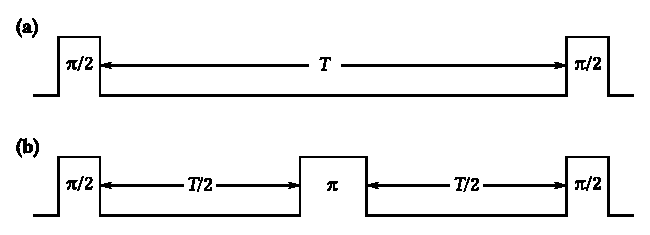
\includegraphics{figures_precreated/sequences.eps}}
    \caption{
    Timeline of the experiment for \textbf{(a)} the regular Ramsey sequence, and \textbf{(b)} the Ramsey sequence with spin echo.}
    \label{fig:bec-noise:visibility:sequences}
\end{figure}

The first protocol is the regular Ramsey sequence, depicted schematically in \figref{bec-noise:visibility:sequences},~(a): a $\pi/2$-pulse is applied by an electromagnetic coupler, creating a non-equilibrium superposition of components $\ket{1}$ and $\ket{2}$.
Mathematically, it means that coupling terms in~\eqnref{bec-noise:mean-field:cgpes-simplified} or in~\eqnref{bec-noise:wigner:single-particle-H} are enabled for a period of time equal to $t_{\mathrm{pulse}} = \theta / \Omega$, where $\theta = \pi/2$, and the Rabi frequency of the oscillator in this experiment was $\Omega = 350\un{Hz}$.
Since this pulse is short as compare to the total evolution time, it was simulated via the application of the rotation matrix~\eqnref{bec-noise:mean-field:rotation-matrix}.

During the further evolution of the system the components experience complex dynamics, separating and merging periodically~\cite{Mertes2007}.
This, in turn, leads to periodic dephasing and self-rephasing of the \abbrev{bec} components.
After some period of the free evolution the second $\pi/2$-pulse is applied, transforming the phase difference between the two components in the superposition into the population difference which can be imaged.
Many such experiments are performed with different free evolution times, contributing one time-point each, because the imaging effectively destroys the \abbrev{bec}.
A more detailed description of the experiment can be found in~\cite{Egorov2011} and in M.~Egorov's PhD thesis~\cite{Egorov2012}.

The simulations in this and the following sections used the plane wave basis (see \appref{bases} for details) and a $64\times8\times8$ spatial grid.
The integration was performed using a low-dissipation 4th-order Runge-Kutta algorithm (see \appref{numerical} for details).

The rephasing cycles can be represented by a common interferometric quantity --- the fringe contrast, or visibility:
\begin{eqn}
\label{eqn:bec-noise:visibility:visibility}
    \mathcal{V}
    = \frac{2 \left| \int \langle \Psiop_1^\dagger \Psiop_2 \rangle \upd \xvec \right|}%
        {\int \langle \Psiop_1^\dagger \Psiop_1 + \Psiop_2^\dagger \Psiop_2 \rangle \upd \xvec},
\end{eqn}
where the denominator is just the total number of atoms in the system.
This quantity can be shown to be the envelope curve of the population fringes produced by the second $\pi/2$-pulse in the experiment.
In the mean-field model the required correlations are calculated simply as
\begin{eqn}
    \tilde{n}
    & = \langle \Psiop_1^\dagger \Psiop_2 \rangle \approx \Psi_1^* \Psi_2, \\
    n_j
    & = \langle \Psiop_j^\dagger \Psiop_j \rangle \approx \Psi_j^* \Psi_j.
\end{eqn}
In the Wigner representation we have to make the correlations symmetrically-ordered first, and then~\eqnref{wigner-bec:fpe-bec:moments} gives us
\begin{eqn}
    \tilde{n}
    & = \langle \Psiop_1^\dagger \Psiop_2 \rangle
    = \langle \symprod{ \Psiop_1^\dagger \Psiop_2 } \rangle
    \approx \Psi_1^* \Psi_2, \\
    n_j
    & = \langle \Psiop_j^\dagger \Psiop_j \rangle
    = \langle \symprod{ \Psiop_j^\dagger \Psiop_j }
        - \frac{\delta_{\restbasis_j}(\xvec, \xvec)}{2} \rangle
    \approx \pathavg{ \Psi_j^* \Psi_j } - \frac{M}{2V},
\end{eqn}
where we used the fact that $\delta_{\restbasis_j}(\xvec, \xvec) \equiv M / V$ in the plane wave basis, where $M$ is the number of modes (for the grid we use $M = 64 \times 8 \times 8 = 4096$), and $V$ is the volume of the simulation area.

\begin{figure}
    \centerline{%
    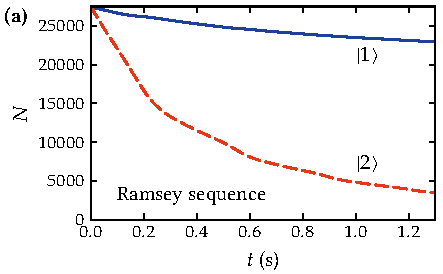
\includegraphics{figures_generated/bec_noise/ramsey_single_run_pop.pdf}%
    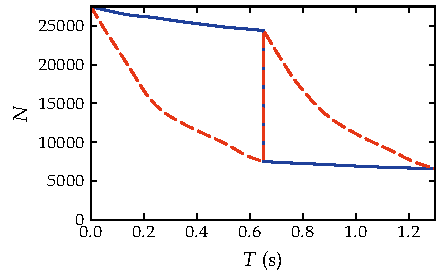
\includegraphics{figures_generated/bec_noise/echo_single_run_pop.pdf}}

    \caption{Numerically simulated population of components $\ket{1}$ (blue solid lines) and $\ket{2}$ (red dashed lines) in \textbf{(a)} Ramsey and \textbf{(b)} spin echo sequences.}

    \label{fig:bec-noise:visibility:population}
\end{figure}

\begin{figure}
    \centerline{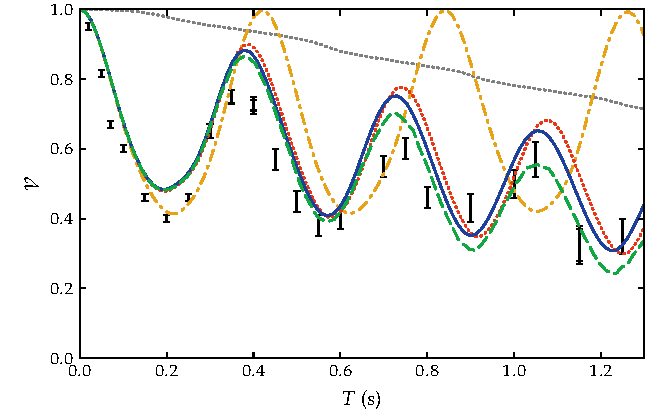
\includegraphics{figures_generated/bec_noise/ramsey_visibility_short.pdf}}

    \caption{
    Comparison of experimental and numerically simulated interferometric contrast at the end of a regular Ramsey sequence with the evolution time $t$.
    Experimental results (black bars) are shown in comparison with the results given by the mean-field model (green dotted line), truncated Wigner method (red dashed line), and truncated Wigner with technical noises included (blue solid line).
    The mean-field results with losses turned off (yellow dash-dotted line) and the population-dependent visibility limit~\eqnref{bec-noise:visibility:limit} (grey dotted line) are included as a reference.}

    \label{fig:bec-noise:visibility:ramsey-visibility}
\end{figure}

The visibility can serve as a good example of the differences introduced by taking into account losses, quantum effects, and technical noises in the simulation of the experiment.
The inclusion of these factors in the simulation of the Ramsey sequence is demonstrated in~\figref{bec-noise:visibility:ramsey-visibility}.
The experimental results and their uncertainties are shown as the black bars in the figure.

The simplest model --- the mean-field \abbrev{cgpe}s~\eqnref{bec-noise:mean-field:cgpes-simplified} with losses turned off --- gives results that are completely off base: the visibility is completely restored during rephasings (yellow dash-dotted lines in the figure).
This is to be expected, as the theoretical limit of visibility
\begin{eqn}
\label{eqn:bec-noise:visibility:limit}
    \mathcal{V}_{\mathrm{max}}
    = \frac{2 \sqrt{N_1 N_2}}{N_1 + N_2},
\end{eqn}
where $N_1$ and $N_2$ are populations before the second $\pi/2$-pulse, equals to $1$ in this case, and there are no other limiting factors.

But in the experiment in question the losses are present and are significantly asymmetrical, as shown in~\figref{bec-noise:visibility:population},~(a).
With the populations typical for the experiment (tens of thousands of atoms or less) the two-body loss process in $\ket{2}$ is significantly stronger than the three-body one in $\ket{1}$.
This makes the theoretical limit~\eqnref{bec-noise:visibility:limit} decrease with time, as the dotted grey line in~\figref{bec-noise:visibility:ramsey-visibility} shows.
The resulting mean-field prediction with the inclusion of nonlinear losses (green dotted lines) is much closer to the experimental data.

The application of the \abbrev{sde}s~\eqnref{bec-noise:wigner:sde} obtained with the Wigner method (red dashed lines) has little effect on the short-time visibility (although it becomes more important at longer times, as we will see later in~\figref{bec-noise:visibility:visibility-long}).
The Wigner results can be further adjusted to account for the noise introduced by the final measurement and non-ideal coupling (blue solid lines), which will be explained in detail in the next section.

The final agreement with the experiment is still not ideal, and the explanation of this difference is an open question.
Candidate factors include finite temperature effects and interaction with the surrounding cloud of non-condensed atoms.

\begin{figure}
    \centerline{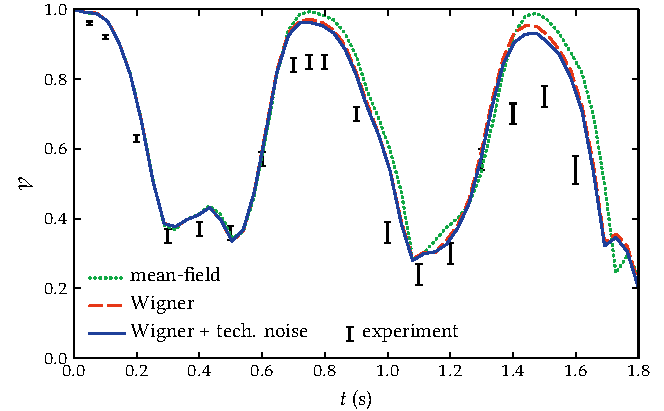
\includegraphics{figures_generated/bec_noise/echo_visibility_short.pdf}}

    \caption{Comparison of experimental and numerically simulated interferometric contrast at the end of a spin echo sequence with the evolution time $t$.
    Experimental results (black bars) show the final visibility value for a single spin echo sequence with the full evolution time $t$ as compared with the predictions from the mean-field model (green dotted line), truncated Wigner method (red dashed line), and truncated Wigner with technical noises included (blue solid line).}

    \label{fig:bec-noise:visibility:echo-visibility}
\end{figure}

The asymmetricity introduced by the difference in loss rates can be compensated by periodically swapping the populations of the two components by a ``spin echo'' coupler pulse of the length $\pi$.
The simplest, yet already very effective, variant is to apply the $\pi$-pulse in the middle of the evolution, as illustrated by~\figref{bec-noise:visibility:sequences},~(b).
With this additional pulse by the end of a single experimental sequence the populations of two components become equal again, as shown in~\figref{bec-noise:visibility:population},~(b), setting the theoretical visibility limit~\eqnref{bec-noise:visibility:limit} back to $1$.

The mean-field model predicts the full recovery of the visibility even at long evolution times, which is inconsistent with the experiment, as seen in~\figref{bec-noise:visibility:echo-visibility}.
On the other hand, the quasiprobability model qualitatively predicts the decay of visibility with time.
Same as in the case of the regular Ramsey sequence, the predictions of the simulation can be improved by including the technical noise.

\begin{figure}
    \centerline{%
    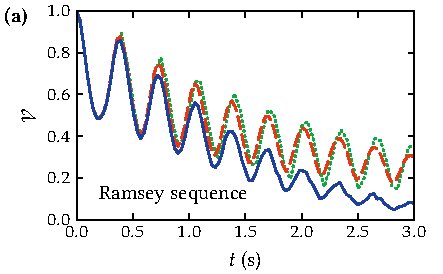
\includegraphics{figures_generated/bec_noise/ramsey_visibility_long.pdf}%
    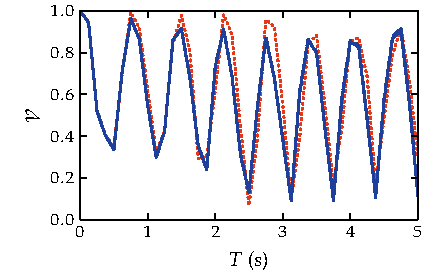
\includegraphics{figures_generated/bec_noise/echo_visibility_long.pdf}}

    \caption{Numerically simulated interferometric contrast for \textbf{(a)} a Ramsey sequence, and \textbf{(b)} a spin echo sequence at longer times.
    Mean-field (green dotted lines), truncated Wigner (red dashed lines) and truncated Wigner with technical noises (blue solid lines) are plotted.}

    \label{fig:bec-noise:visibility:visibility-long}
\end{figure}

The simulations can be performed for longer times, as shown in~\figref{bec-noise:visibility:visibility-long}.
The difference between the mean-field and the truncated Wigner approach becomes more clear in~\figref{bec-noise:visibility:visibility-long},~(a), where the truncated Wigner predicts the significant decrease in the amplitude of the rephasing oscillations, caused by the quantum noise.
One must remember though that at such times the simulated atom densities become too low due to losses and violate the truncation validity criterion~\eqnref{wigner-bec:truncation:delta-condition}, thus making the predictions less reliable.

% =============================================================================
\section{Phase noise}
% =============================================================================

Another important characteristic of a \abbrev{bec} interferometry experiment is the phase noise, which is connected with the visibility.
We will discuss it based on the same experiment~\cite{Egorov2011,Egorov2012} as in the previous section.

While in the simulation we can measure the visibility~\eqnref{bec-noise:visibility:visibility} simply by calculating a second-order moment, experimentalists do not have the luxury of knowing the wavefunctions of the components.
Instead, multiple runs of the Ramsey sequence with the same evolution time are performed, with the second $\pi/2$-pulse having a different phase lag $\phi$ each time.
The quantity that can be measured in the experiment is the normalized atom difference
\begin{eqn}
    P_z = \frac{N_2^\prime - N_1^\prime}{N_1^\prime + N_2^\prime},
\end{eqn}
where $N_1^\prime$ and $N_2^\prime$ are populations of the components obtained by imaging after the second $\pi/2$-pulse.
Using the rotation matrix~\eqnref{bec-noise:mean-field:rotation-matrix} it can be shown that $P_z$ can be expressed in terms of wave operators before the second $\pi/2$-pulse as
\begin{eqn}
    P_z(\phi)
    = - \frac{2}{N_1 + N_2} \Imag \left(
        e^{-i\phi} \int \langle \Psiop_1^\dagger \Psi_2 \rangle \upd\xvec
        \right).
\end{eqn}
One can notice that the integral of the second order moment in this expression is the same as in~\eqnref{bec-noise:visibility:visibility}, and is also normalized on the total population.
Therefore if we vary $\phi$ in the experiment, the resulting $P_z(\phi)$ can be fit with a sine function, and its amplitude will give us the visibility $\mathcal{V}$.

\begin{figure}
    \centerline{%
    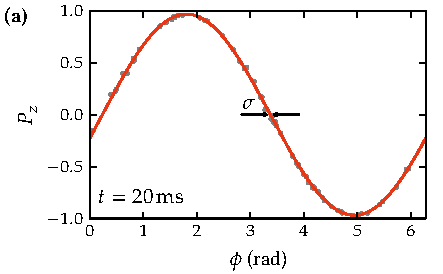
\includegraphics{figures_generated/bec_noise/illustration_noise_20ms.pdf}%
    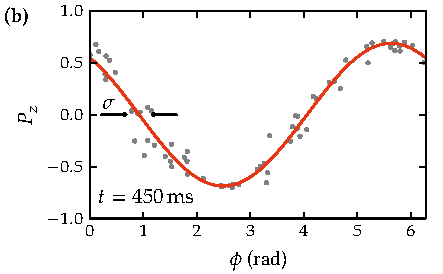
\includegraphics{figures_generated/bec_noise/illustration_noise_450ms.pdf}}

    \caption{Phase noise in experimental measurements of visibility at \textbf{(a)}~$t = 20\un{ms}$ and \textbf{(b)}~$t = 450\un{ms}$.
    Black dots illustrate possible results obtained in a single run of the Ramsey interferometry experiment.}%endcaption

    \label{fig:bec-noise:phase-noise:illustration}
\end{figure}

In practice, naturally, the measurement of $P_z$ is affected by various sources of technical noise.
As a result, the measured points are displaced from the ideal curve.
In the experiment in question three such noise sources were identified.
First, the length of $\pi/2$-pulses varied throughout the exeprimental runs with an estimated standard deviation of $\Delta \theta = 0.02\un{rad}$ (caused by the drift of the Rabi frequency $\Omega$).
The phase of the coupler also had an uncertainty caused by the MW frequency instability that grew with time as $\Delta \phi / t = 0.5\un{rad/s}$.
Finally, the imaging technique used to measure populations $N_1^\prime$ and $N_2^\prime$ resulted in an uncertainty of $\Delta N / N = 0.023$.
These factors can be trivially added to the simulations: first two at the moment of the application of the rotation matrix~\eqnref{bec-noise:mean-field:rotation-matrix}, by adding a random factor to the length $\theta$ and the phase $\phi$, and the third one by adding a random factor to the populations $N_1$ and $N_2$ produced by integrating the corresponding moments of wavefunctions.

The result is is illustrated in~\figref{bec-noise:phase-noise:illustration}, with the ``experimental'' points emulated this way plotted agains a sine fit, for two different evolution times.
The base simulation is the truncated Wigner one for the regular Ramsey sequence from the previous section.
The standard deviation of the horizontal distance $\sigma$ of the experimental results from the fitting curve is called the phase noise.
The amplitude of the curve, in turn, is taken to be the predicted visibility accounting for the technical noises (see~\figref{bec-noise:visibility:ramsey-visibility} and~\figref{bec-noise:visibility:echo-visibility} in the previous section).

\begin{figure}
    \centerline{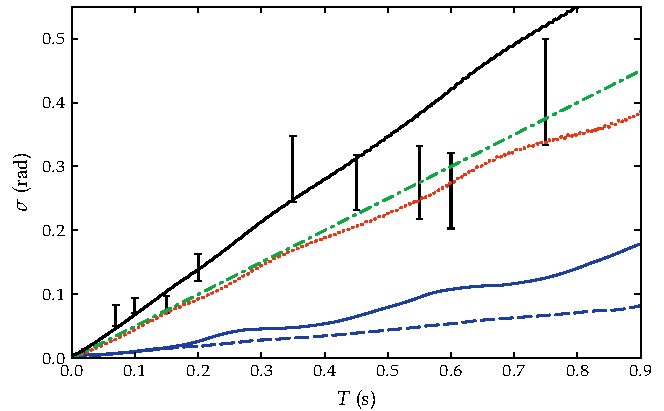
\includegraphics{figures_generated/bec_noise/ramsey_noise.pdf}}

    \caption{Comparison of experimental (black bars) and numerically simulated phase noise at the end of a Ramsey sequence with the evolution time $t$.
    The truncated Wigner predictions with (blue solid line) and without (red dashed line) the inclusion of technical noises is shown.}%endcaption

    \label{fig:bec-noise:phase-noise:ramsey-phnoise}
\end{figure}

A comparison of the phase noise with the experimental data for the regular Ramsey sequence is shown in~\figref{bec-noise:phase-noise:ramsey-phnoise}.
The experimental parameters are the same as in the previous section.
The effect of quantum noise (red dashed line) is noticeable, but not very large as compared to the compound effect of the technical noises (blue solid line).
There seems to be a lot of room for the improvement of the apparatus until the measurements hit the ``hard'' limit of the quantum noise.

\begin{figure}
    \centerline{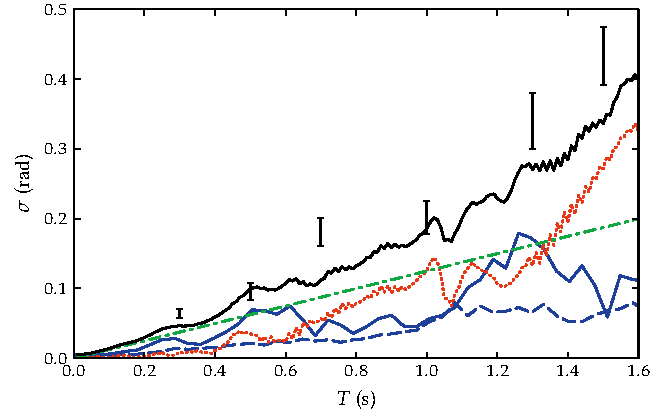
\includegraphics{figures_generated/bec_noise/echo_noise.pdf}}

    \caption{Comparison of experimental (black bars) and numerically simulated phase noise at the end of a spin echo sequence with the evolution time $t$.
    The truncated Wigner predictions with (blue solid line) and without (red dashed line) the inclusion of technical noises is shown.}%endcaption

    \label{fig:bec-noise:phase-noise:echo-phnoise}
\end{figure}

Phase noise in a spin echo sequence can be estimated in the same way.
The reported MW frequency instability for this experiment was $\Delta \phi / t = 0.125\un{rad/s}$.
As~\figref{bec-noise:phase-noise:echo-phnoise} shows, even after the inclusion of the technical noise, there is some disagreement with the experimental data.
This may be caused by the systematic error introduced by the truncation, or possibly by some additional source of technical noise.

One may notice that the total noise shown in~\figref{bec-noise:phase-noise:ramsey-phnoise} and~\figref{bec-noise:phase-noise:echo-phnoise} is lower than the one reported in~\cite{Egorov2011,Egorov2012}.
This is the result of the honest calculation of the total noise (in essence, we simulate the actual experimental measurement procedure), as opposed to the post-factum combination of noise from the technical sources with the Wigner results.

% =============================================================================
\section{Conclusion}
% =============================================================================

The examples in this chapter demonsrate that the truncated Wigner approach gives correct long-time predictions of quantum effects for the system comprised of large number of atoms.
Both of these features, large atom numbers and long time-scales, are essential to accurate interferometric measurements.
The predictions remains correct even despite multimode dynamical motion in three dimensions and substantial losses of most of the condensate atoms.
On longer time-scales, the experimental accuracy is limited by technical noises, and we have no data for comparisons.


% =============================================================================
\chapter{Squeezing in 3D BEC interferometry}
% =============================================================================

This chapter contains squeezing results from \cite{Opanchuk2012}.

% =============================================================================
\chapter{EPR entanglement in the 2-well system}
% =============================================================================

This chapter contains EPR results from \cite{Opanchuk2012a}.

% =============================================================================
\chapter{Probabilistic representation of Bell inequalities violation}
\label{cha:bell-ineq}
% =============================================================================

In this final chapter we will diverge from the main topic~--- the Wigner representation~---, and briefly discuss other quasiprobability representations.
In particular we will be interested in their ability to model such an inherent quantum property of quantum systems as entanglement~\cite{Einstein1935}, and the consequent violation of Bell inequalities~\cite{Bell1964}.
The possibility of this is often discarded because of the famous Feynman's lecture~\cite{Feynman1982}, where he posed a question \textit{``Can quantum systems be probabilistically simulated by a classical computer?''}, and his final answer was \textit{``If ... there's no hocus-pocus, the answer is certainly, No!''}.
His argument was based on the proof that Bell violations cannot be modeled probabilistically~\cite{Bell1964}.

But it turns out that the positive phase-space distributions of quantum optics~\cite{Husimi1940,Drummond1980,Hillery1984,Gardiner2004} are capable of such simulations, owing to the extended codomains of allowed observables as compared to those considered by Bell.
Namely, observables in phase-space distributions can have a continous range of values extending beyond the set of discrete expected values for the physical quantity, and, furthermore, their values can be complex~\cite{Reid1986}.
The expectations of such observables correspond to physical quantities only when integrated with the phase-space distribution as a weight.
This method of simulation is analogous to the weak measurement strategy, or \abbrev{povm} (positive operator valued measure)~\cite{Aharonov1988}, which has been experimentally demonstrated recently~\cite{Goggin2011}.

% acknowledgement
The idea of demonstrating the violation of Bell inequalities using quasiprobability representations belongs to M.~D.~Reid.


% =============================================================================
\section{Cooperative states}
% =============================================================================

A Bell inequality sets a limit on observable correlations in a physical system that obeys a local hidden variable theory (\abbrev{lhv})~\cite{Bell1964,Clauser1969}.
This is a classical theory where the results of the measurements are functions of local detector settings and a hidden parameter $\lambda$.
Thus, values measured by two spatially separated observers, $A$ and $B$ (for Alice and Bob, as they are usually denoted), can be expressed as $A(a, \lambda)$ and $B(b, \lambda)$, where $a$ and $b$ are Alice's and Bob's detector settings.
Possible correlations are defined probabilistically as
\begin{eqn}
\label{eqn:bell-ineq:cooperative:lhv}
    C(A,B)
    = \int_{\Lambda} A(a, \lambda) B(b, \lambda) P(\lambda) \upd\lambda.
\end{eqn}
Experimental values $A$ and $B$ are usually encoded as either $1$ or $-1$ in a binary experiment.
The Bell theorem derives inequalities that any such correlations in a \abbrev{lhv} theory must satisfy.
Quantum mechanics violates these inequalities, thus ruling out \abbrev{lhv} theories.


% =============================================================================
\subsection{Quantum state}
% =============================================================================

In this section we will consider Bell violations in cooperative states with $N$ photon pairs, similar to those demonstrated experimentally by Clauser~\cite{Clauser1969}, Aspect \textit{et~al}~\cite{Aspect1982}, and Zeilinger \textit{et~al}~\cite{Weihs1998}.
The quantum state in question is
\begin{eqn}
\label{eqn:bell-ineq:cooperative:state}
    \vert N \rangle
    = \frac{%
        \left(
            \hat{a}_{1+}^{\dagger} \hat{a}_{2+}^{\dagger}
            + \hat{a}_{1-}^{\dagger} \hat{a}_{2-}^{\dagger}
        \right)^{N} \vert 0 \rangle%
        }{N! \left( N+1 \right)^{1/2}},
\end{eqn}
where $N$ is the number of photon pairs, indices $1$ and $2$ denote the propagation direction, and $+$ and $-$ stand for the polarization direction.
These states are generated in certain types of optical parametric down-conversion experiments, and it has proved difficult to obtain a direct, loophole free violation of a Bell inequality, owing to detector inefficiencies~\cite{Cabello2007,Larsson1998,Larsson2001}.
However, these issues are not significant for the simulations in this thesis since we are considering an ideal experiment.

We define the intensity correlations to be~\cite{Drummond1983}
\begin{eqn}
\label{eqn:bell-ineq:cooperative:G}
    G^{IJ}(\gamma,N)
    = \langle N \vert
        \hat{A}^{I}(1,\hat{\avec}_{1})
        \hat{A}^{J}(\gamma,\hat{\avec}_{2})
        \vert N \rangle,
\end{eqn}
where $\gamma$ is a linear combination parameter related to the polarizer angle, and auxiliary functions are introduced so that:
\begin{eqn}
    \hat{A}^{J}(\gamma,\hat{\avec}_{k})
    ={} & \left(
            \sqrt{\gamma} \hat{a}_{k-}^{\dagger}
            + \sqrt{1-\gamma} \hat{a}_{k+}^{\dagger}
        \right)^{J}
        \left(
            \sqrt{\gamma} \hat{a}_{k-}
            + \sqrt{1-\gamma} \hat{a}_{k+}
        \right)^{J}, \\
    \hat{A}^{J}(\infty,\hat{\avec}_{k})
    ={} & :\left(
        \hat{a}_{k-}^{\dagger} \hat{a}_{k-}
        + \hat{a}_{k+}^{\dagger}\hat{a}_{k+}
        \right)^{J}: .
\end{eqn}

For $N$ photon pairs, the Bell-type inequality is then known to be of the form~\cite{Drummond1983}
\begin{eqn}
\label{eqn:bell-ineq:cooperative:violation}
    \Delta(\theta) = 3g(\theta) - g(3\theta) - 2 \le 0,
\end{eqn}
where
\begin{eqn}
    g_{N}^{J}(\theta) = G^{JJ}(\cos^{2}\theta,N) / G^{JJ}(\infty,N).
\end{eqn}
This expression generalizes the usual Clauser, Horne, Shimony and Holt (\abbrev{chsh})~\cite{Clauser1969} and Bell expressions to a multi-particle form.
The quantum mechanical prediction for $g_{N}^{J}$ has especially simple form of $g_{N}^{N}(\theta)=\cos^{2N}\theta$ for the cases $J=N$, $N=1,2$ which we have simulated.
This gives the violation of
\begin{eqn}
\label{eqn:bell-ineq:cooperative:violation-1}
    \Delta_{\mathrm{1\, pair}}(\theta)
    = 3\cos^{2}\theta - \cos^{2}3\theta - 2
\end{eqn}
for the two-particle case, which corresponds to the usual two-particle experiment originally proposed by Bell.
For the four-particle case, the violation can be found to be
\begin{eqn}
\label{eqn:bell-ineq:cooperative:violation-2}
    \Delta_{\mathrm{2\, pairs}}(\theta)
    = 3\cos^{4}\theta - \cos^{4}3\theta - 2.
\end{eqn}


% =============================================================================
\subsection{Positive-P representation}
% =============================================================================

We simulate the violation~\eqnref{bell-ineq:cooperative:violation} using the positive-P representation~\cite{Drummond1980,Gardiner2004}.
In essence, it is an exact expansion of an arbitrary density matrix of bosons with a positive probability distribution $P(\balpha, \bbeta)$, such that the expectation of an observable $\hat{O}$ is
\begin{eqn}
\label{eqn:bell-ineq:cooperative:pos-P-expectation}
    \langle \hat{O} \rangle
    = \int \upd^2 \balpha\, \upd^2 \bbeta\,
        P(\balpha,\bbeta)
        \langle \bbeta^* \vert \hat{O} \vert \balpha \rangle /
        \langle \bbeta^* \vert \balpha \rangle,
\end{eqn}
where $\vert\balpha\rangle$ is a multimode coherent state.
The positive P-representation, therefore, corresponds exactly to the definition of a physical weak measurement~\cite{Aharonov1988}, with the initial state $\vert\balpha\rangle$ and the final postselected state $\vert\bbeta\rangle$ occurring with probability $P(\balpha,\bbeta)$.
The standard form we use is also known to be measurable using multiple beam-splitter operations~\cite{Agarwal1994}.

The expression above looks very similar to~\eqnref{bell-ineq:cooperative:lhv}, given by \abbrev{lhv}.
The fundamental difference, which allows the correlations obtained from the positive-P distribution to violate Bell inequalities, is that the quantities being sampled can be complex numbers of any magnitude.
Only after the weighted averaging with the probability distribution $P$ they give the value of the observable.

For an arbitrary moment of creation and annihilation operators $\hat{O}(\avec^\dagger, \avec)$, the expectation is calculated as
\begin{eqn}
\label{eqn:bell-ineq:cooperative:moment-expectation}
    \langle \hat{O} \rangle
    = \int \upd^2 \balpha\, \upd^2 \bbeta\,
        P(\balpha,\bbeta)
        O(\bbeta, \balpha),
\end{eqn}
where $O$ is a function produced as a result of replacing any $\hat{a}_i$ with $\alpha_i$ and $\hat{a}_i^\dagger$ with $\beta_i$ in $\hat{O}$.
For example, the mode population $\langle \hat{a}_i^\dagger \hat{a}_i \rangle$ corresponds to the moment $\beta_i \alpha_i$, which is, in general, complex, and only its expectation is real.

The quantum state~\eqnref{bell-ineq:cooperative:state} we are interested in corresponds to the positive-P distribution~\cite{Drummond1983}
\begin{eqn}
\label{eqn:bell-ineq:cooperative:pos-P}
    P(\balpha,\bbeta)
    ={} & \left\{
        \frac{ |
            (\beta_{1+} + \alpha_{1+}^{*}) (\beta_{2+} + \alpha_{2+}^{*})
            + (\beta_{1-} + \alpha_{1-}^{*}) (\beta_{2-} + \alpha_{2-}^{*}) |^{2N}}{%
            (2\pi)^{8} (N+1) (N!)^{2}2^{4N}}
        \right\} \\
        & \times \exp \left(
            -\frac{ |\balpha|^{2} + |\bbeta|^{2}}{2}
        \right).
\end{eqn}
This distribution exists and has a positive, probabilistic behavior for all values of $N$.
Note that it is not unique, and it may be possible to find other expressions that correspond to the same quantum state, but have better sampling properties.


% =============================================================================
\subsection{Sampling}
% =============================================================================

In order to illustrate our point better, we simulate the measurement of the operator~\eqnref{bell-ineq:cooperative:G} using the Monte-Carlo method: we sample the distribution~\eqnref{bell-ineq:cooperative:pos-P} and calculate the weighted average~\eqnref{bell-ineq:cooperative:pos-P-expectation}.

We sample this distribution by transforming it to a form where we can use the well-known von Neumann rejection algorithm.
Performing the variable change
\begin{eqn}
\label{eqn:bell-ineq:cooperative:mu-lambda}
    \bmu = \frac{\balpha - \bbeta^*}{2},\quad
    \blambda = \frac{\balpha + \bbeta^*}{2},
\end{eqn}
and grouping the components of $\blambda$ and $\bmu$ as
\begin{eqn}
\label{eqn:bell-ineq:cooperative:ab-delta-ab}
    \Avec & = [ \lambda_{1+}, \lambda_{1-} ],\quad
    \Bvec = [ \lambda_{2+}, \lambda_{2-} ],\\
    \delta\Avec & = [ \mu_{1+}, \mu_{1-} ],\quad
    \delta\Bvec = [ \mu_{2+}, \mu_{2-} ],
\end{eqn}
we can separate the positive-P function into independent parts as
\begin{eqn}
    P(\Avec, \Bvec, \delta\Avec, \delta\Bvec)
    = P^\prime(\Avec, \Bvec) G(\delta\Avec) G(\delta\Bvec).
\end{eqn}
Here $G$ is a $4$-component Gaussian distribution with the variance $\sigma^2 = 1/2$ in each real component
\begin{eqn}
    G(\delta\Avec)
    = \frac{1}{\pi^2} e^{-|\delta\Avec|^2},
\end{eqn}
and $P^\prime$ is the distribution core with a reduced number of variables
\begin{eqn}
    P^\prime(\Avec, \Bvec)
    = \left(
            \frac{ |\Avec \cdot \Bvec |^{2N} }{\pi^4 (N+1) (N!)^2}
        \right)
        e^{-|\Avec|^2 - |\Bvec|^2},
\end{eqn}

The Gaussian parts can be sampled exactly using conventional methods, while the distribution core requires requires an application of rejection sampling.
Since $|\Avec\cdot\Bvec| \le |\Avec| |\Bvec|$, $P^\prime$ can be bounded as
\begin{eqn}
    P^\prime(\Avec, \Bvec) \le F(\Avec) F(\Bvec),
\end{eqn}
where
\begin{eqn}
    F(\Avec)
    = \frac{|\Avec|^2N}{\pi^2 \sqrt{N+1} N!} e^{-|\Avec|^2}.
\end{eqn}
The bounding function $F$ will be used as a probability distribution in the rejection sampling, so it must be normalised on $1$.
In order to do that, we notice that
\begin{eqn}
    \int |\Avec|^{2N} e^{-|\Avec|^{2}} \upd^2 \Avec
    & = S_{k-1}(1) \int_0^{\infty} r^{2N+k-1} \exp(-r^{2}) \upd r \\
    & = \frac{1}{2} \Gamma(N+k/2) S_{k-1}(1),
\end{eqn}
where $k$ is the number of components in $\Avec$ (in our case $\Avec$ contains two complex numbers, so $k=4$), and $S_{k-1}(R)$ is the surface area of a $k$-dimensional ball:
\begin{eqn}
    S_{k-1}(r) = \frac{2\pi^{k/2} r^{k-1}}{\Gamma(k/2)}.
\end{eqn}
Thus, the normalisation coefficient is
\begin{eqn}
    M
    = \int F(\Avec) \upd^2 \Avec
    = \frac{\Gamma(N+2)}{2\pi^{2}\sqrt{N+1}N!} \times \frac{2\pi^{2}}{\Gamma(2)}
    = \sqrt{N+1},
\end{eqn}
and $F(\Avec) = M F^\prime(\Avec)$, where $F^\prime$ is a probability distribution
\begin{eqn}
    F^\prime(\Avec)
    = \frac{|\Avec|^{2N}}{\pi^2 (N+1)!} e^{-|\Avec|^2}.
\end{eqn}

The distribution $F^\prime$, in turn, can be represented as a product of two independent distributions~\cite{Gupta1997}:
\begin{eqn}
    F^\prime(\Avec)
    \equiv F^\prime(r,\nvec)
    = S_{k-1}(r) g(r^2) U(\nvec)
    = R(r) U(\nvec),
\end{eqn}
where $r = |\Avec|$, $\nvec$ is a unit vector on a $k$-dimensional sphere, and $U=1/S_{k-1}(1)$ is a uniform distribution of vector directions (or, in other words, a uniform distribution on the surface of a $k$-dimensional ball).
The latter can be sampled using the Marsaglia algorithm~\cite{Marsaglia1972} (sampling a vector of $k$ normally distributed random numbers and normalising it on $1$).
In order to sample the distribution $R$, we have to do another variable change, $r^{2}\rightarrow x$:
\begin{eqn}
    R(x)
    & = \frac{1}{2\sqrt{x}} S_{k-1}(\sqrt{x}) g(x) \\
    & = \frac{1}{2\sqrt{x}}
        \frac{2\pi^{k/2} x^{(k-1)/2}}{\Gamma(k/2)}
        \frac{x^{N}}{\pi^2 (N+1)!} e^{-x} \\
    & = \frac{x^{N+1}}{(N+1)!} e^{-x}.
\end{eqn}
The result is exactly the gamma-distribution with the scale $\alpha = N + 2$, for which an efficient sampling method exists~\cite{Marsaglia2000}.

Combining it all together, the rejection algorithm for sampling the probability distribution~\eqnref{bell-ineq:cooperative:pos-P} consists of the following steps:
\begin{enumerate}
\item Sample two squared lengths $|\Avec|^2$ and $|\Bvec|^2$ using the gamma distribution with the scale $N+2$.
\item Sample two directions $\nvec_A$ and $\nvec_B$ using the Marsaglia algorithm.
\item Combine squared lengths and directions into $\Avec$ and $\Bvec$.
\item Sample $u$ from the uniform distribution on $[0,1)$.
\item If $u > P^\prime(\Avec,\Bvec) / (M^2 F^\prime(\Avec) F^\prime(\Bvec))$, reject the sample and start over.
\item Sample the real components of $\delta\Avec$ and $\delta\Bvec$ independently using Gaussian distributions with the variance $1/2$ and combine them with $\Avec$ and $\Bvec$ to get $\balpha$ and $\bbeta$ using~\eqnref{bell-ineq:cooperative:ab-delta-ab} and~\eqnref{bell-ineq:cooperative:mu-lambda}.
\end{enumerate}
The resulting phase-space coordinates $\balpha$ and $\bbeta$ can be now used to get a sample of any moment of creation and annihilation operators using the formula~\eqnref{bell-ineq:cooperative:moment-expectation}.


% =============================================================================
\subsection{Results}
% =============================================================================

\begin{figure}
    \centerline{%
    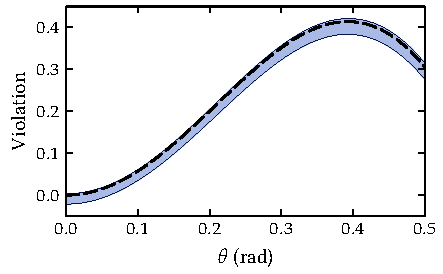
\includegraphics{figures_generated/bell/cooperative_N1.pdf}%
    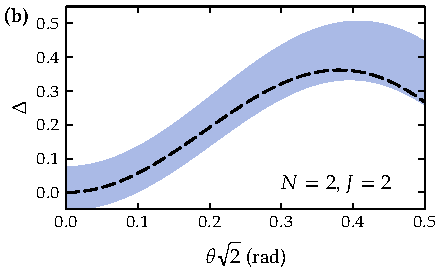
\includegraphics{figures_generated/bell/cooperative_N2.pdf}}

    \caption[Simulated Bell violation for cooperative states]{
    Simulated Bell violation $\Delta$ as a function of the relative polarizer angle $\theta$ for \textbf{(a)} one, and \textbf{(b)} two photon pairs using the positive-P distribution with \textbf{(a)} $2^{21}$ and \textbf{(b)} $2^{25}$ samples.
    The filled area corresponds to the estimated sampling error around the mean of $\Delta(\theta)$ for the sampled state, while the dashed line is the exact quantum mechanical prediction of this value.}%endcaption

    \label{fig:bell-ineq:cooperative:violation}
\end{figure}

Using the sampling method described in the previous subsection, we can now sample the positive-P distribution~\eqnref{bell-ineq:cooperative:pos-P} and calculate the violation~\eqnref{bell-ineq:cooperative:violation}.
We do that for the two-particle case $N=J=1$, and also for the four-particle case $N=J=2$, which has been observed experimentally~\cite{Howell2002}.
The results are plotted in~\figref{bell-ineq:cooperative:violation}, together with the analytical predictions~\eqnref{bell-ineq:cooperative:violation-1} and~\eqnref{bell-ineq:cooperative:violation-2}.
The second case requires significantly more samples to achieve a small enough sampling error, but it is clear that in both cases we were able to demonstrate the violation which is beyond the sampling error range.

% =============================================================================
\section{GHZM states}
\label{sec:bell-ineq:ghz}
% =============================================================================

We also perform mesoscopic Schr\"odinger cat state simulations, corresponding to recent ion-trap experiments with $M$ qubits.
These states violate a genuine multipartite Bell inequality, which means that it is impossible to confine the Bell violation to a microscopic part of the state.
Such inequalities require the measurement of all possible correlation functions at the highest order available.
We find two distinct scaling laws for the total computational difficulty, as measured by the number of samples required to obtain a given sampling error.

To understand the ultimate scaling properties of probabilistic sampling methods, we have also simulated higher order correlations that violate multipartite Bell inequalities.
These are found in quantum states that display Bell violations with $M$ observers, not just two.
The most well-known examples are the multimode entangled Greenberger-Horne-Zeilinger-Mermin (\abbrev{ghzm}) states~\cite{Greenberger1989,Mermin1990}, corresponding to ``Schr\"odinger Cat'' states.
Therefore, we considered \abbrev{ghzm} states, which describe $M$ spin-$\frac{1}{2}$ particles or qubits:
\begin{eqn}
\label{eqn:bell-ineq:ghz:state}
    \vert\Phi\rangle
    = \frac{1}{\sqrt{2}} \left(
        \ket{\uparrow\ldots\uparrow}
        + e^{i\phi} \ket{\downarrow\ldots\downarrow}
    \right).
\end{eqn}
Here $\ket{\uparrow}$ and $\ket{\downarrow}$ denote spin-up or spin-down particles in the $z$-direction.
As well as being of deep significance in quantum physics, such mesoscopic states have been generated in recent ion-trap experiments~\cite{Rowe2001,Leibfried2005,Monz2011}.

Quantum paradoxes are obtained on measuring an operator $\hat{A}$ which is defined as a linear combination of $2^{M}$ distinct $M$-th order correlation functions:
\begin{eqn}
\label{eqn:bell-ineq:ghz:operator}
    \hat{A}
    = \prod_{j=1}^{M} \left(
            \hat{\sigma}_j^x
            + i \hat{\sigma}_j^y
        \right),
\end{eqn}
where $s_j \in {-1, +1}$, and $\hat{\sigma}_j^x$ and $\hat{\sigma}_j^y$ are the Pauli spin operators acting on the $j$-th qubit.
We consider the constraints imposed by a \abbrev{lhv} on the expectation $A_{\lambda}(\phi) \equiv \langle \Phi(\phi) \vert \hat{A} \vert \Phi(\phi) \rangle_\lambda$ (where $\langle \rangle_{\lambda}$ stands for the expectation under \abbrev{lhv} assumptions) as compared to the predictions for these expectations given by quantum mechanics, $A_{\mathrm{QM}}(\phi) \equiv \langle \Phi(\phi) \vert \hat{A} \vert \Phi(\phi) \rangle$.

Mermin~\cite{Mermin1990} originally proved that for the phase difference $\phi=\pi/2$, \abbrev{qm} predicts that
\begin{eqn}
    \Imag A_{\mathrm{QM}}(\pi / 2)
    = 2^{M - 1},
\end{eqn}
while the \abbrev{lhv} bounds are
\begin{eqn2}
    \Imag A_{\lambda}(\pi / 2) & \le 2^{M/2},\quad & M\,\mathrm{is\,even}, \\
    \Imag A_{\lambda}(\pi / 2) & \le 2^{(M-1)/2},\quad & M\,\mathrm{is\,odd}.
\end{eqn2}
Ardehali~\cite{Ardehali1992} then proved that for $\phi=\pi$, the predictions are
\begin{eqn}
    -\Real A_{\mathrm{QM}}(\pi)
    = 2^{M - 1},
\end{eqn}
and
\begin{eqn2}
    -\Real A_{\lambda}(\pi) & \le 2^{(M-1)/2},\quad & M\,\mathrm{is\,even}, \\
    -\Real A_{\lambda}(\pi) & \le 2^{M/2},\quad & M\,\mathrm{is\,odd}.
\end{eqn2}
Here we transformed the original expressions given by Ardehali to the equivalent ones that use our definition of the target operator~\eqnref{bell-ineq:ghz:operator}.

It is clear that the Mermin inequalities are stronger for odd $M$, and the Ardehali ones are stronger for even $M$ (in particular, for $M = 2$ the Mermin inequalities are not even violated by \abbrev{qm}).
Therefore for our sampling tests in this section we will use the strongest of two inequalities, and the corresponding phase difference in the \abbrev{ghzm} state, for every $M$:
\begin{eqn2}
    F & = -\Real A_{\lambda}(\pi),\quad & M\,\mathrm{is\,even},\\
    F & = \Imag A_{\lambda}(\pi / 2),\quad & M\,\mathrm{is\,odd}.
\end{eqn2}
Consequently, for \abbrev{qm} and \abbrev{lhv} predictions we get the uniform \abbrev{qm} prediction $F_{\mathrm{QM}} = 2^{M - 1}$ and the inequality
\begin{eqn}
\label{eqn:bell-ineq:ghz:general-ineq}
    F_{\lambda} \le 2^{(M-1)/2}.
\end{eqn}
The relative violation can thus be made arbitrarily big to compensate for any imperfections in the measurements.


% =============================================================================
\subsection{Positive-P representation}
% =============================================================================

The na\"ive approach to the sampling of the state~\eqnref{bell-ineq:ghz:state} is to use the P-representation, same as we did in the previous section.
In general, spin-up and spin-down states are represented as $\ket{\uparrow}\equiv\ket{10}$ and $\ket{\downarrow}\equiv\ket{01}$, where $\ket{0}$ and $\ket{1}$ are number states, which allows for straightforward application of Pauli spin operators.

But for our particular choice of the target operator~\eqnref{bell-ineq:ghz:operator}, we can choose a simplified representation, which will halve the dimensionality of the resulting phase space: $\ket{\uparrow}\equiv\ket{0}$ and $\ket{\downarrow}\equiv\ket{1}$.
Since every term of $\hat{A}$ contains only one spin operator per qubit, it can be expressed in terms of creation and annihilation operators by replacing the spin operators with
\begin{eqn}
    \hat{\sigma}_j^x = \hat{a}_j + \hat{a}_j^\dagger,\quad
    \hat{\sigma}_j^y = \frac{1}{i} (\hat{a}_j - \hat{a}_j^\dagger),
\end{eqn}
from which the equivalent function of $\balpha$ and $\bbeta$ in P-representation immediately follows.

The P-representation of the target state is obtained with the canonical formula~\cite{Drummond1980}
\begin{eqn}
    P[\hat{\rho}]
    = \left( \frac{1}{4\pi^2} \right)^M
        \exp\left(
            -\frac{|\balpha -\bbeta^*|^2}{4}
        \right)
        \bra{\frac{1}{2} \left( \balpha + \bbeta^* \right)}
        \hat{\rho}
        \ket{\frac{1}{2} \left( \balpha + \bbeta^* \right)},
\end{eqn}
which for $\rho \equiv \ket{\Phi} \bra{\Phi}$ gives
\begin{eqn}
    P
    = \frac{1}{2 \pi^{2M}} e^{-|\bmu|^2} e^{-|\blambda^2|}
        \left|
            \prod_{j=1}^M \lambda_j + 1
        \right|^2,
\end{eqn}
where we have performed the variable change~\eqnref{bell-ineq:cooperative:mu-lambda}
\begin{eqn}
    \bmu = \frac{\balpha - \bbeta^*}{2},\quad
    \blambda = \frac{\balpha + \bbeta^*}{2}.
\end{eqn}

The sampling is performed using the rejection method with bounding $P$ as
\begin{eqn}
    P
    \le \frac{1}{2 \pi^{2M}} e^{-|\bmu|^2} e^{-|\blambda^2|}
        \left( \prod_{j=1}^M |\lambda_j|^2 + 1 \right).
\end{eqn}
Therefore, $P$ can be sampled using a combination of independent samples from Gaussian and gamma distributions, and then conditionally rejecting samples, as described in the previous section.

The phase space in this representation has $4M$ dimensions.
This can be further improved by using a specialized representation, allowing us to reduce the sampling error significantly, thus making the states with larger values of $M$ accessible for sampling.


% =============================================================================
\subsection{SU(2)-Q representation}
% =============================================================================

% acknowledgement
The theoretical derivation of the SU(2)-Q representation was performed by L.~E.~C.~Rosales-Z\'arate.
In this subsection we will briefly describe the framework of the representation, and apply it to our target state.

The positive-P representation does not impose any restrictions on the phase space, including the number states with population more than $1$ in the calculation of moments.
While it does not affect the calculated observable, it does increase the sampling error.
For the cases when we know that the system consists of binary states, more suitable representations exist.

We will consider a Q-representation~\cite{Husimi1940} for SU(2) coherent states~\cite{Arecchi1972,Zhang1990}:
\begin{eqn}
    \kket{\zvec}
    = \prod_{j=1}^{M} \left(
            \ket{\downarrow}_j + z_j \ket{\uparrow}_j
        \right),
\end{eqn}
where $z_j$ are complex numbers.
The SU(2)-Q function is the expectation value of the density operator over the SU(2) coherent states and is defined explicitly in a normalized form as:
\begin{eqn}
    Q[\hat{\rho}]
    = \left(
        \prod_{j=1}^M \frac{2}{\pi (1 + |z_j|^2)^3}
    \right) \bbra{\zvec} \hat{\rho} \kket{\zvec}.
\end{eqn}
For the target \abbrev{ghzm} state~\eqnref{bell-ineq:ghz:state}, the function takes the form of a probability distribution
\begin{eqn}
\label{eqn:bell-ineq:ghz:ghz-Q}
    Q
    = \frac{1}{2} \prod_{j=1}^M
        \frac{2}{\pi (1 + |z_j|^2)^3}
        \left|
            \prod_{j=1}^M z_j + e^{-i \phi}
        \right|^2
\end{eqn}

The sampling is again performed using the rejection method with bounding $Q$ as
\begin{eqn}
    Q
    \le \frac{1}{2} \prod_{j=1}^M
        \frac{2}{\pi (1 + |z_j|^2)^3}
        \left(
            \prod_{j=1}^M |z_j|^2 + 1
        \right),
\end{eqn}
and using the inverse sampling on both terms.
The expectation of $\hat{A}$ can be shown to be
\begin{eqn}
    A_{\mathrm{SU(2)-Q}}
    = \int
        6^M \prod_{j=1}^M \frac{z_j^*}{1 + |z_j|^2}
        Q(\zvec) \upd^2 \zvec.
\end{eqn}


% =============================================================================
\subsection{Results}
% =============================================================================

\begin{figure}
    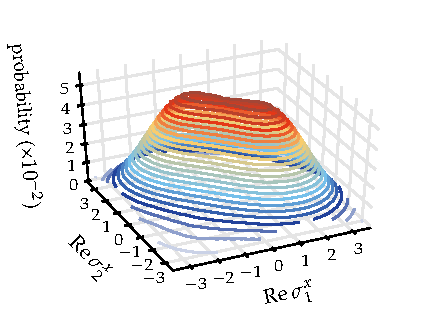
\includegraphics{figures_generated/bell/distribution_P1.pdf}%
    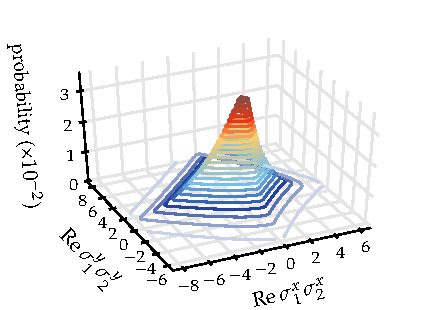
\includegraphics{figures_generated/bell/distribution_P2.pdf}\\
    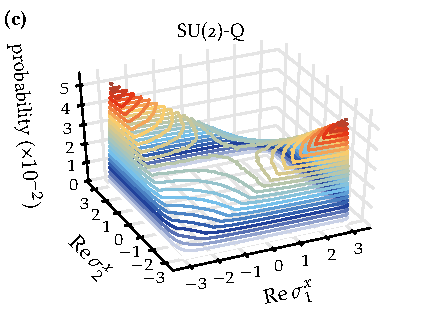
\includegraphics{figures_generated/bell/distribution_Q1.pdf}%
    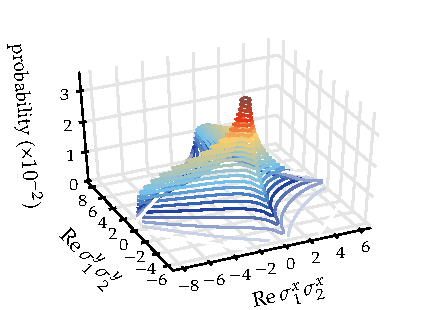
\includegraphics{figures_generated/bell/distribution_Q2.pdf}

    \caption[Correlations of first- and second-order moments in a Bell inequality]{
    Correlations for the different parts of the inequality~\eqnref{bell-ineq:ghz:general-ineq-M2}, in case of \textbf{(a, b)} positive-P and \textbf{(c, d)} SU(2)-Q representations, $10^8$ samples.}%endcaption

    \label{fig:bell-ineq:ghz:correlations}
\end{figure}

The difference between the positive-P and SU(2)-Q representations (and their difference from \abbrev{lhv} theories) can be illustrated on the inequality~\eqnref{bell-ineq:ghz:general-ineq} for $M = 2$:
\begin{eqn}
\label{eqn:bell-ineq:ghz:general-ineq-M2}
    - \langle \hat{\sigma}_1^x \hat{\sigma}_2^x \rangle_{\lambda}
    + \langle \hat{\sigma}_1^y \hat{\sigma}_2^y \rangle_{\lambda}
    \le \sqrt{2}.
\end{eqn}
The real parts of the correlations in this expression for both representations used are plotted in~\figref{bell-ineq:ghz:correlations}.

The main feature of quasiprobability representations is apparent: neither of them limits the value of $\Real \sigma_1^x$ or $\Real \sigma_2^x$ to the range $[-1, 1]$ as would happen in a \abbrev{lhv} theory.
This means that the Bell theorem does not apply to these results because the sampled values differ from their physical equivalents.
Moreover, the plots for the SU(2)-Q show that in this representation the correlations are more peaked, and also do not have exponential tails as the ones in the positive-P representation.
This, in addition to the reduced phase space dimensionality, allows the sampling with SU(2)-Q representation for high values of $M$.

\begin{figure}
    \centerline{%
    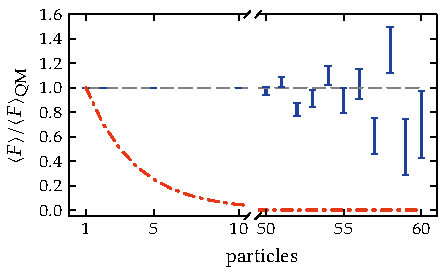
\includegraphics{figures_generated/bell/ghz_violations.pdf}%
    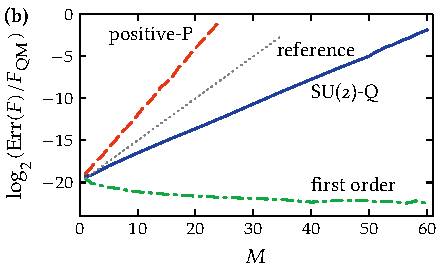
\includegraphics{figures_generated/bell/ghz_errors.pdf}}

    \caption[Violation of Bell inequality in \abbrev{ghzm} states]{
    Violations of the inequality~\eqnref{bell-ineq:ghz:general-ineq} for multi-particle \abbrev{ghzm} states.
    \textbf{(a)} Blue bars show the expectation $F$ simulated using the SU(2)-Q representation, with the length of the bars corresponding to the sampling error.
    The values of expectations and errors are normalized by the quantum mechanical prediction for the corresponding $M$.
    The horizontal grey dashed line gives the quantum prediction.
    The red dash-dotted line is the \abbrev{lhv} prediction, which gives a Bell violation when the expectation $F$ is above this line.
    \textbf{(b)} Relative sampling errors for $F$ simulated using the positive-P (red dashed line) and SU(2)-Q (blue solid line) representations.
    Sampling errors for a first order correlation (total number of ``spin-ups'') in the SU(2)-Q representation are plotted as a green dashed line.
    The grey dotted reference line $\log_2 \mathrm{error} \propto M / 2$ shows the point at which the sampling errors would give scaling properties as slow as an experimental measurement.}%endcaption

    \label{fig:bell-ineq:ghz:violation}
\end{figure}

The results of such sampling are shown in~\figref{bell-ineq:ghz:violation}.
We used seven nVidia Tesla M2090 \abbrev{gpu}s to generate $10^{12}$ samples of the distribution~\eqnref{bell-ineq:ghz:ghz-Q} and calculate the required correlation for the values of $M$ up to $60$, and these samples were used to test the inequality~\eqnref{bell-ineq:ghz:general-ineq}.
This corresponds to measurement of $10^{18}$ distinct sixtieth order correlation functions.
As~\figref{bell-ineq:ghz:violation},~(a) demonstrates, Bell violations were verified in all cases, although closer to $M=60$ the sampling error grew almost enough to invalidate the results.
Larger values of $M$ would require more samples.

We also investigated the growth of sampling errors for $F$ with the positive-P and SU(2)-Q representations, as shown in~\figref{bell-ineq:ghz:violation},~(b).
In order to have some reference for comparisons, we also plotted the sampling error for the total number of ``spin-ups''
\begin{eqn}
    N = \langle\sum_{j=1}^M (\hat{\sigma}_j^z + 1 )/2 \rangle.
\end{eqn}
This low-order spin correlation requires a linearly growing amount of measurements in the experiment as compared to the exponentially growing amount for $F$.
As the plot shows, the sampling error for $N$ even slowly decreases as $M$ grows.
This explains why low-order correlations could be efficiently sampled in previous work, for much larger Hilbert spaces than the ones studied here.

On the other hand, high-order correlations showed exponentially growing sampling error.
In case of positive-P the relative error scales as $2^{4M/5}$, which with the chosen number of samples, produces Bell violations only up to $M=25$.
The SU(2)-Q representation shows much better results with the relative error scaling as $2^{M/3}$, so the time taken by the simulation at constant error scales as $2^{2M/3}$.
An experiment measuring the same quantity would take time proportional to $2^M$ since it would have to perform measurements for exponentially many settings.
Thus, the probabilistic sampling of the SU(2)-Q function scales better than experiment for high-order correlations.

These results show that probabilistic sampling is a perfectly viable technique both for low- and high-order correlations.
Low-order correlations are the ones most commonly measured, and sampling errors in these are insensitive to scaling up to mesoscopic sizes.
Correlations of the same order as the system size are still exponentially hard, but a carefully chosen quasiprobability representation can give an exponential advantage over experimental scaling.

% =============================================================================
\section{Conclusion}
% =============================================================================



% =============================================================================
\chapter{Conclusion}
\label{cha:conclusion}
% =============================================================================

In this thesis we introduced the functional Wigner transformation formally.
We proved the required theorems from Wirtinger and functional calculi, and used them to derive the essential properties of the Wigner transformation: sequential transformation of operator products, and the correspondence between operator expectations and moments of the Wigner functional.

We then applied this framework to the exact operator equation governing the dynamics of a \abbrev{bec} and showed how to transform it into the equivalent partial differential equation.
An approximation (Wigner truncation) was introduced, which allowed us to simplify this equation further, and turn it into a set of \abbrev{sde}s for trajectories in the phase space.
All of this was done while keeping the functional nature of equations intact and retaining the inherent mode cutoff of field operators and wavefunctions, which is unavoidable in numerical simulations.

On the whole, it allowed us to link the coefficients and terms in the master equation directly with those of \abbrev{sde}s, resulting in a simple method of numerical simulation of \abbrev{bec} dynamics.
This method includes the effect of nonlinear losses in a natural way, is capable of producing any high-order correlations without changes to the initial state or the propagation, and is highly parallelisable.
The latter is a huge advantage in the modern world of multi-core and multi-node computations and the recent advent of general calculations on \abbrev{gpu}s.
In particular, the use of modern \abbrev{gpu}s allowed us to simulate the dynamics of hundreds of thousands of atoms with thousands of modes with a high degree of accuracy on a desktop in the order of hours.

As a simple test of the truncation accuracy, we applied the multimode form of the Wigner representation to a two-mode system, for which an exact quantum mechanical description is possible.
We have shown that the Wigner method gives correct results in the characteristic time frame, with systematic errors much lower than what is testable in an experiment.

We then used the truncated Wigner method to model some recent \abbrev{bec} interferometry experiments, both local and reported by other experimental teams.
The method showed good agreement with the experimental results for such important observables as interferometric contrast (a second-order correlation), phase noise and degree of spin squeezing (fourth-order correlations).
The method allows one to account for experimental imperfections (measurement and apparatus noises) naturally, which greatly increases the accuracy of predictions.

In the last chapter we considered a more broad topic of the ability of phase space methods to simulate quantum mechanical systems, and their differences from \abbrev{lhv} theories.
We showed that, due to weaker restrictions on the codomains of the moments that correspond to physical observables, such methods are indeed capable of demonstrating such essential quantum mechanical properties as the violation of Bell inequalities.
We were able to calculate the correlations involving every particle in the system in highly entangled \abbrev{ghzm} states for up to $60$ particles.
This result is far beyond the capabilities of current experimental techniques.

\centerline{\asterism}

In conclusion, we have shown that the truncated Wigner method is a convenient and fast tool that can be used to plan the future experiments, and to get better insight into the existing ones.
There is, of course, still a lot of room for further improvement.

First, we have only used coherent initial states and zero temperature for our simulations.
While it is a reasonable first approximation, for some experiments this may not be acceptable.
The obvious next step here is to include finite-temperature initial conditions using Bogoliubov modes~\cite{Steel1998,Sinatra2002,Ruostekoski2005,Isella2006,Blakie2008}.
During the simulation, the validity of the truncation needs to be estimated more accurately than by using the condition~\eqnref{wigner-bec:truncation:delta-condition}.
This condition turns out to be, in fact, more of a guideline as there are examples of good agreement with the exact methods even when it is not satisfied.
More accurate test can be performed by calculating the quantum correction~\cite{Polkovnikov2010}.

Speaking about phase space methods generally, despite demonstrating excellent results in sampling static quantum states, they often struggle in simulating the dynamics of these systems.
Positive-P is known to display exponentially growing sampling error because of the redundant dimensions it uses.
In some cases, this can be neutralized by using a gauge-P representation~\cite{Deuar2002,Deuar2005a}, or adding a projection.

Finally, it is possible to make the Wigner representation positive in the same way it was done for the P representation~\cite{Plimak2001}.
The applicability of this ``positive-Wigner'' representation to various simulation problem is yet to be investigated.


\appendix
\counterwithin{lemma}{chapter}
\counterwithin{theorem}{chapter}
\counterwithin{definition}{chapter}

% =============================================================================
\chapter{Wirtinger calculus}
\label{cha:appendix:c-numbers}
% =============================================================================

Formally, a function of complex variable has to be holomorphic in order to be complex differentiable.
In many cases, however, it is enough to have less strict ``physicists'\,'' complex differentiation rules, which only requre the function's real and complex part to be differentiable, without imposing additional constraints.
Such rules were developed by Wirtinger~\cite{Wirtinger1927}; further extension to vectors and matrices was performed by Hj{\o}rungnes and Gesbert~\cite{Hjorungnes2007}.
A very good review and a thorough description of their application was made by Kreutz-Delgado~\cite{Kreutz-Delgado2009}.
This section will outline Wirtinger differentiation rules and provide some lemmas based on them, which, in turn, are going to be used in the further Appendices, and in the main body of the thesis.


% =============================================================================
\section{Differentiation}
% =============================================================================

We will start from the definition of the differentiation:

\begin{definition}
\label{def:c-numbers:wirtinger}
	For a complex variable $z \equiv x + iy$, and a function $f(z) \equiv u(x, y) + iv(x, y)$
	\begin{eqn*}
		\left( \frac{\upd f(z)}{\upd z} \right)
		= \frac{1}{2} \left(
			\frac{\upd f}{\upd x} - i \frac{\upd f}{\upd y}
		\right).
	\end{eqn*}
\end{definition}

One can easily check that if $f(z)$ is holomorphic, this definition is equivalent to the standard complex differentiation.
Wirtinger differentiation is quite intuitive in the sense that it obeys all the basic rules associated with a real-valued differentiation:

\begin{theorem}
\label{thm:c-numbers:diff-properties}
	For any $f(z)$ with differentiable real and complex parts, Wirtinger differentiation obeys sum, product, quotient, and chain differentiation rules.
	The latter one is applied as if $f(z)$ was a function of two independent variables $z$ and $z^*$:
	\begin{eqn*}
		\frac{\upd f(g(z))}{\upd z}
		= \frac{\upd f}{\upd g} \frac{\upd g}{\upd z}
			+ \frac{\upd f}{\upd g^*} \frac{\upd g^*}{\upd z}.
	\end{eqn*}
\end{theorem}

Some important functions we will encounter in this thesis are not holomorphic.
Therefore, hereinafter we will use Wirtinger differentiation unless explicitly stated otherwise,
along with notation $\upd f/\upd z$ (to avoid confusion with regular partial derivatives).
Consequently, by ``differentiability'' we will mean the property used in the above theorem, i.e. the existence of partial derivatives of $\Real f$ and $\Imag f$ over real and complex axis.

It is convenient to connect symbolic rules for Wirtinger differentiation with the rules for common real-valued differentiation.

\begin{theorem}
\label{thm:c-numbers:independent-vars}
	If a function $f(z)$ can be expanded into series of $z^n (z^*)^m$, then $\upd f/\upd z$ and $\upd f/\upd z^*$ can be calculated as partial derivatives of the function $f$ expressed in terms of $z$ and $z^*$, over $z$ and $z^*$ respectively:
	\begin{eqn*}
		\frac{\upd f(z)}{\upd z} \equiv \frac{\upp f(z, z^*)}{\upp z},
		\quad
		\frac{\upd f(z)}{\upd z^*} \equiv \frac{\upp f(z, z^*)}{\upp z^*}.
	\end{eqn*}
\end{theorem}
\begin{proof}
We will prove the first identity.
Without loss of generality, we can consider $f(z) = z^r (z^*)^s$.
First, one can easily prove (by transition to real values) that $\upd (z z^*)/\upd z = z^*$ and $\upd (z z^*)/\upd z^* = z$.
Let us assume that the identity is true for some $r$ and $s$; then, using the product rule,
\begin{eqn}
	\frac{\upd}{\upd z} (z^{r+1} (z^*)^s)
	& = \frac{\upd}{\upd z} (z z^r (z^*)^s)
		= z^r (z^*)^s + z \frac{\upd}{\upd z} (z^r (z^*)^s) \\
	& = z^r (z^*)^s + r z z^{r-1} (z^*)^s
		= (r + 1) z^r (z^*)^s.
\end{eqn}
By induction, the statement is true for any natural $r$ and $s$, and it is obviously true if $r = 0$ or $s = 0$, which proves the theorem.
\end{proof}

The chain differentiation rule in \thmref{c-numbers:diff-properties} and the above theorem give rise to the common notation used in conjunction with Wirtinger differentiation.
In order to emphasize the ``independent'' behavior of $z$ and $z^*$, function arguments are often written as $f(z, z^*)$, even though technically they are not independent.
We will use such notation throughout the thesis.


% =============================================================================
\section{Integration}
% =============================================================================

Wirtinger differentiation can be paired with the somewhat more common integration over the complex plane:

\begin{definition}
\label{def:c-numbers:integration}
	For a complex $z = x + iy$
	\begin{eqn*}
		\int \upd^2 z \equiv \int_{-\infty}^{\infty} \int_{-\infty}^{\infty} \upd x\, \upd y.
	\end{eqn*}
\end{definition}

This definition allows us to prove an analogue of one of the properties of the Fourier transform expressed in terms of Wirtinger differentiation:

\begin{lemma}
\label{lmm:c-numbers:fourier-of-moments}
	For a complex $\lambda$ and any non-negative integers $r$ and $s$
	\begin{eqn*}
		\int \upd^2\alpha\, \alpha^r (\alpha^*)^s \exp(-\lambda \alpha^* + \lambda^* \alpha)
		= \pi^2
			\left( -\frac{\upd}{\upd \lambda^*} \right)^r
			\left( \frac{\upd}{\upd \lambda} \right)^s
			\delta(\Real \lambda) \delta(\Imag \lambda).
	\end{eqn*}
\end{lemma}
\begin{proof}
First, by changing a variable in the integral and using known Fourier transform relations, we can prove that for real $x$ and $v$, and non-negative integer $n$
\begin{eqn}
\label{eqn:c-numbers:fourier-real}
	\int\limits_{-\infty}^{\infty} \upd v\, v^n \exp(\pm 2 i x v)
	= \pi (\mp i / 2)^n \delta^{(n)}(x).
\end{eqn}
Note that we have explicitly written integration limits here;
they are swapped when we change the variable in the first integral.

Denoting $\alpha = u + iv$ and $\lambda = x + iy$, we can expand the initial expression as
\begin{eqn}
	& \int \upd^2\alpha\, \alpha^r (\alpha^*)^s \exp(-\lambda \alpha^* + \lambda^* \alpha) \\
	& = \int \upd u\, \upd v\, \exp(2ivx - 2iuy)
		\sum_{m=0}^r \binom{r}{m} u^m (iv)^{r-m}
		\sum_{n=0}^s \binom{s}{n} u^n (-iv)^{s-n} \\
	& = \sum_{m=0}^r \sum_{n=0}^s \binom{r}{m} \binom{s}{n}
		i^{r-m} (-i)^{s-n}
		\int \upd u\, u^{m+n} \exp(2ivx)
		\int \upd v\, v^{r-m+s-n} \exp(-2iuy).
\end{eqn}
Applying~\eqnref{c-numbers:fourier-real} and grouping differentials:
\begin{eqn}
	& = \pi^2 \sum_{m=0}^r \sum_{n=0}^s \binom{r}{m} \binom{s}{n}
		i^{r-m} (-i)^{s-n}
		(-i/2)^{m+n} \delta^{(m+n)}(y)
		(i/2)^{r-m+s-n} \delta^{(r-m+s-n)}(x) \\
	& = \pi^2
		\sum_{m=0}^r \binom{r}{m}
			\frac{1}{2^r}
			(-i \upd / \upd y)^m
			(-\upd / \upd x)^{r-m}
		\sum_{n=0}^s \binom{s}{n}
			\frac{1}{2^s}
			(-i \upd / \upd y)^n
			(\upd / \upd x)^{s-n}
		\delta(y) \delta(x).
\end{eqn}
Collapsing sums and recognizing \defref{c-numbers:wirtinger}:
\begin{eqn}
	& = \pi^2
		\left( \frac{1}{2} (-i \upd / \upd y - \upd / \upd x) \right)^r
		\left( \frac{1}{2} (-i \upd / \upd y + \upd / \upd x) \right)^s
		\delta(y) \delta(x) \\
	& = \pi^2
		\left( -\frac{\upd}{\upd \lambda^*} \right)^r
		\left( \frac{\upd}{\upd \lambda} \right)^s
		\delta(\Real \lambda) \delta(\Imag \lambda).
		\qedhere
\end{eqn}
\end{proof}

It can be proved by expansion in real variables that the formally written rule of integration by parts works for the integral from \defref{c-numbers:integration}:
\begin{eqn}
	\int \upd z\, f \frac{\upd g}{\upd z}
	= \int \upd z \frac{\upd (fg)}{\upd z} - \int \upd z \frac{\upd f}{\upd z} g.
\end{eqn}
Integration by parts will be used extensively in further proofs, and we will need two lemmas that will handle the first term in the right part of the above expression.

\begin{lemma}
\label{lmm:c-numbers:zero-integrals}
	For a square-integrable $f(\lambda, \lambda^*)$, and a complex $\alpha$
	\begin{eqn*}
		\int \upd^2\lambda
			\frac{\upd}{\upd \lambda} \left(
				\exp(-\lambda \alpha^* + \lambda^* \alpha)
				f(\lambda, \lambda^*)
			\right)
		& = 0, \\
		\int \upd^2\lambda
			\frac{\upd}{\upd \lambda^*}
			\left(
				\exp(-\lambda \alpha^* + \lambda^* \alpha)
				f(\lambda, \lambda^*)
			\right)
		& = 0.
	\end{eqn*}
\end{lemma}
\begin{proof}
From the square-integrability of $f$ it follows that $\lim_{\Real \lambda \rightarrow \infty} = 0$ and $\lim_{\Imag \lambda \rightarrow \infty} = 0$, so the statement of the lemma can be proved by transforming to real variables and integrating.
\end{proof}

\begin{lemma}
\label{lmm:c-numbers:zero-delta-integrals}
	For a bounded $f(\lambda, \lambda^*)$
	\begin{eqn*}
		\int \upd^2\lambda
			\frac{\upd}{\upd \lambda} \left(
				f(\lambda, \lambda^*)
				\left( \frac{\upd}{\upd \lambda} \right)^s
				\left( -\frac{\upd}{\upd \lambda^*} \right)^r
				\delta(\Real \lambda) \delta(\Imag \lambda)
			\right)
		& = 0, \\
		\int \upd^2\lambda
			\frac{\upd}{\upd \lambda^*}
			\left(
				f(\lambda, \lambda^*)
				\left( \frac{\upd}{\upd \lambda} \right)^s
				\left( -\frac{\upd}{\upd \lambda^*} \right)^r
				\delta(\Real \lambda) \delta(\Imag \lambda)
			\right)
		& = 0.
	\end{eqn*}
\end{lemma}
\begin{proof}
Proved straightforwardly by expanding integrals in real values, separating variables and integrating, using the fact that any derivative of the delta function is zero on the infinity.
\end{proof}

% =============================================================================
\chapter{Functional calculus}
\label{cha:appendix:func-calculus}
% =============================================================================

The definitions of differentiation and integration from \appref{c-numbers} can be extended to operate on functions and functionals.
This proved to be a useful tool in the derivation of the functional Wigner transformation and expressing accompanied results, as it helps encapsulate bases and mode populations inside wave functions and field operators.
It has been introduced (among other places) in most of the papers treating functional extensions of quasiprobability with varying level of detail.
The most extensive description was made by Dalton~\cite{Dalton2011}.
Although, while these papers cover the foundations quite well, they are missing several important results which are essential for this thesis, and which will be therefore proved in this Appendix.


% =============================================================================
\section{Functional spaces and projections}
% =============================================================================

We will assume we are provided with an arbitrary orthonormal basis $\fullbasis$, consisting of functions $\phi_{\nvec}(\xvec)$, where $\xvec \in \mathbb{R}^D$ is a $D$-dimensional coordinate vector, and $\nvec \in \fullbasis$ is a mode identifier.
The exact nature of a mode identifier is irrelevant; we only require it to have an equivalence relation defined, and be enumerable.
For example, for a three-dimensional harmonic potential, the mode identifier will be a tuple $(k,l,m)$ of three non-negative integers.

Orthonormality and completeness conditions for basis functions are, respectively,
\begin{eqns}
\label{eqn:func-calculus:basis}
	\int\limits_A \phi_{\nvec}^*(\xvec) \phi_{\mvec}(\xvec) \upd\xvec
	& = \delta_{\nvec\mvec}, \\
	\sum_{\nvec \in \fullbasis} \phi_{\nvec}^*(\xvec) \phi_{\nvec}(\xvec^\prime)
	& = \delta(\xvec^\prime - \xvec),
\end{eqns}
where the integration area $A$ depends on the basis set (for example, $A$ is the whole space for harmonic oscillator modes, and a box for plane waves).
Hereinafter we assume that the integration $\int \upd\xvec$ is always performed over $A$, unless explicitly stated otherwise. In addition, to avoid clutter, for functions of coordinates the argument list will be omitted (i.e. $f(\xvec) \equiv f$ and $f(\xvec^\prime) \equiv f^\prime$) except where it is necessary for clarity.

Various functions can be combined from all, or the certain subset of basis modes by means of a composition:

\begin{definition}
\label{def:func-calculus:composition}
	For some subset of the full basis $\restbasis \subseteq \fullbasis$, the composition transformation creates a function from a vector of mode populations:
	\begin{eqn*}
		\mathcal{C}_{\restbasis}(\balpha)
		= \sum_{\nvec \in \restbasis} \phi_{\nvec} \alpha_{\nvec}.
	\end{eqn*}
	Decomposition transformation, correspondingly, creates a vector of populations out of a function:
	\begin{eqn*}
		(\mathcal{C}_{\restbasis}^{-1}[f])_{\nvec}
		= \int \upd\xvec \phi_{\nvec}^* f,\,{\nvec} \in \restbasis.
	\end{eqn*}
\end{definition}

For any subset of the full basis, there is a certain subspace of functions that can be obtained by composing modes from this subset only.

\begin{definition}
	For some subset of the full basis $\restbasis \subseteq \fullbasis$, $\mathbb{F}_{\restbasis} \equiv (\mathbb{R}^D \rightarrow \mathbb{C})_{\restbasis}$ is a space of all functions of coordinates, which can be obtained from $\mathcal{C}_{\restbasis}$.
	In other words, such functions consist only of modes from $\restbasis$.
	We denote $\mathbb{F}_{\fullbasis} \equiv \mathbb{F}$.
\end{definition}

Using this definition, the type of composition and decomposition transformations can be written as
\begin{eqn}
		\mathcal{C}_{\restbasis} \in \mathbb{C}^{|\restbasis|} \rightarrow \mathbb{F}_{\restbasis},\quad
		\mathcal{C}_{\restbasis}^{-1} \in \mathbb{F} \rightarrow \mathbb{C}^{|\restbasis|}
\end{eqn}
Note also that for any $f \in \mathbb{F}_{\restbasis}$ corresponding composition and decomposition are reversible, i.e. $\mathcal{C}_{\restbasis}(\mathcal{C}_{\restbasis}^{-1}[f]) \equiv f$.
We will refer such functions as restricted functions.

The result of any non-linear transformation of a function $f \in \mathbb{F}_{\restbasis}$ is not guaranteed to belong to $\mathbb{F}_{\restbasis}$ and requires explicit projection to be used with other restricted functions from the same subspace $\mathbb{F}_{\restbasis}$:

\begin{definition}
\label{def:func-calculus:projector}
	An arbitrary function can be projected to $\mathbb{F}_{\restbasis}$ using the projection operator:
	\begin{eqn*}
		& \proj{\restbasis} \in \mathbb{F} \rightarrow \mathbb{F}_{\restbasis} \\
		& \proj{\restbasis}[f](\xvec)
		\equiv (\mathcal{C}_{\restbasis}(\mathcal{C}_{\restbasis}^{-1}[f])) (\xvec)
		= \sum_{\nvec \in \restbasis} \phi_{\nvec} \int
			\upd\xvec^\prime\, \phi_{\nvec}^{\prime*} f^\prime.
	\end{eqn*}
	Obviously, $\proj{\fullbasis} \equiv \mathds{1}$.
\end{definition}

Being applied to the delta function, the projection operator produces a restricted delta function:

\begin{definition}
\label{def:func-calculus:restricted-delta}
	The restricted delta function $\delta_{\restbasis} \in \mathbb{F}_{\restbasis}$ is a projected form of standard delta function:
	\begin{eqn*}
		\delta_{\restbasis}(\xvec^\prime, \xvec)
		= \proj{\restbasis}[\delta]
		= \sum_{\nvec \in \restbasis} \phi_{\nvec}^{\prime*} \phi_{\nvec}.
	\end{eqn*}
	Note that in general $\delta_{\restbasis}^*(\xvec^\prime, \xvec) = \delta_{\restbasis}(\xvec, \xvec^\prime)$, so the order of variables is important.
	For a full basis, this definition coincides with the standard delta function: $\delta_{\fullbasis}(\xvec^\prime, \xvec) \equiv \delta(\xvec^\prime - \xvec)$.
\end{definition}

Projection transformation can be, in turn, expressed using the restricted delta function:
\begin{eqn}
	\proj{\restbasis}[f](\xvec) = \int \upd\xvec^\prime \delta_{\restbasis}(\xvec^\prime, \xvec) f^\prime.
\end{eqn}
The conjugate of $\proj{\restbasis}$ is therefore
\begin{eqn}
	(\proj{\restbasis}[f](\xvec))^*
	= \int \upd\xvec^\prime \delta_{\restbasis}^*(\xvec^\prime, \xvec) f^{\prime*}
	= \proj{\restbasis}^* [f^*](\xvec).
\end{eqn}


% =============================================================================
\section{Functional differentiation}
% =============================================================================

Let $\mathcal{F}[f] \in \mathbb{F}_{\restbasis} \rightarrow \mathbb{F}$ be some arbitrary functional operator (not to be confused with quantum mechanical operators) acting on functions from a restricted basis.
Such operator can be as simple as an algebraic function of $f$, for example, $\mathcal{F}[f] = f^2$, but it can also be more complicated.
Note that in general this operator is nor linear, therefore its result is not guaranteed to belong to the same restricted basis as its argument.
Also, since $\mathbb{C}$ is a specific case of $\mathbb{F}$ (a constant function of coordinates), a specific case of a functional operator is a functional $\mathcal{F}[f] \in \mathbb{F}_{\restbasis} \rightarrow \mathbb{C}$).
This means that the calculus described in this section applies to functionals as well.

Composition and decomposition transformations from \defref{func-calculus:composition} define a bijection between a restricted function space $\mathbb{F}_{\restbasis}$ and a vector space of the corresponding dimensionality $\mathbb{C}^{|\restbasis|}$ (where $|\restbasis|$ denotes the cardinality of $\restbasis$).
Therefore any functional operator $\mathcal{F}$ can be alternatively treated as a function of a vector of mode populations and a coordinate vector:
\begin{eqn}
	& F \in \mathbb{C}^{|\restbasis|} \rightarrow \mathbb{F}
		\equiv \mathbb{C}^{|\restbasis|} \rightarrow \mathbb{R}^D \rightarrow \mathbb{C} \\
	& F(\balpha, \xvec) \equiv \mathcal{F}[\mathcal{C}_{\restbasis}(\balpha)](\xvec).
\end{eqn}
Since the operator is not linear, this correspondence in general cannot be expressed in a form of matrix.

Using this correspondence, we can define the differentiation in the space of functional operators:

\begin{definition}
\label{def:func-calculus:func-diff}
	Derivative of a functional operator is
	\begin{eqn*}
		& \frac{\fdelta}{\fdelta f^\prime} \in
		\left(
			\mathbb{F}_{\restbasis} \rightarrow \mathbb{F}
		\right)
		\rightarrow
		\left(
			\mathbb{R}^D \rightarrow \mathbb{F}_{\restbasis} \rightarrow \mathbb{F}
		\right) \\
		& \frac{\fdelta \mathcal{F}[f]}{\fdelta f^\prime}
		= \left.
				\sum_{\nvec \in \restbasis} \phi_{\nvec}^{\prime*}
				\frac{\cwd \mathcal{F}[\mathcal{C}_{\restbasis}(\balpha)]}{\cwd \alpha_{\nvec}}
			\right|_{\balpha = \mathcal{C}_{\restbasis}^{-1}[f]}.
	\end{eqn*}
\end{definition}

Note that the type of the returned operator differs from the argument type: the result depends on two coordinates, not just one.
The second coordinate ($\xvec^\prime$) comes from the function $f^\prime \equiv f(\xvec^\prime)$ we are differentiating by.

This definition may look too elaborate at first, but later in this section we will see that it leads to intuitive consequences, making the functional derivative behave very similar to the Wirtinger derivative from \appref{c-numbers}.
Let us first demonstrate that the definition obeys standard differentiation rules.

\begin{theorem}
	Functional differentiation from \defref{func-calculus:func-diff} obeys sum, product, quotient, and chain differentiation rules.
	The latter one is applied as if $\mathcal{F}[f]$ was a function of two independent variables $f$ and $f^*$:
	\begin{eqn*}
		\frac{\fdelta \mathcal{F}[\mathcal{G}[f]]}{\fdelta f^\prime}
			= \int \upd\xvec^{\prime\prime} \left(
				\frac{\fdelta \mathcal{F}}{\fdelta \mathcal{G}^{\prime\prime}}
				\frac{\fdelta \mathcal{G}}{\fdelta \mathcal{f}^{\prime}}
				+ \frac{\fdelta \mathcal{F}}{\fdelta \mathcal{G}^{\prime\prime*}}
				\frac{\fdelta \mathcal{G}^*}{\fdelta \mathcal{f}^{\prime}}
			\right).
	\end{eqn*}
\end{theorem}
\begin{proof}
First tree rules are proved straightforwardly by substituting $\mathcal{F} + \mathcal{G}$, $\mathcal{F} \mathcal{G}$ and $\mathcal{F} / \mathcal{G}$ into \defref{func-calculus:func-diff}.
To prove the latter, let us substitute $\mathcal{F}[\mathcal{G}]$ into the definition:
\begin{eqn}
\label{eqn:func-calculus:chain-expansion}
	\frac{\fdelta \mathcal{F}[\mathcal{G}[f]]}{\fdelta f^\prime}
		& = \left.
				\sum_{\nvec \in \restbasis} \phi_{\nvec}^{\prime*}
				\frac{\cwd \mathcal{F}[\mathcal{G}[\mathcal{C}_{\restbasis}(\balpha)]]}{\cwd \alpha_{\nvec}}
			\right|_{\balpha = \mathcal{C}_{\restbasis}^{-1}[f]} \\
		& = \left.
				\sum_{\nvec \in \restbasis} \phi_{\nvec}^{\prime*}
				\frac{\cwd \mathcal{F}[\mathcal{C}(\bbeta)]}{\cwd \alpha_{\nvec}}
			\right|_{\bbeta = \mathcal{C}^{-1}[\mathcal{G}[\mathcal{C}_{\restbasis}(\balpha)]]}.
\end{eqn}
Applying the chain rule for Wirtinger derivatives, and recalling the definition of the decomposition transformation:
\begin{eqn}
	\frac{\cwd \mathcal{F}[\mathcal{C}(\bbeta)]}{\cwd \alpha_{\nvec}}
	= \sum_{\mvec \in \fullbasis} \left(
		\frac{\cwd \mathcal{F}[\mathcal{C}(\bbeta)]}{\cwd \beta_{\mvec}}
		\frac{\cwd \beta_{\mvec}}{\cwd \alpha_{\nvec}}
		+ \frac{\cwd \mathcal{F}[\mathcal{C}(\bbeta)]}{\cwd \beta_{\mvec}^*}
		\frac{\cwd \beta_{\mvec}^*}{\cwd \alpha_{\nvec}}
	\right),
\end{eqn}
\begin{eqn}
	\frac{\cwd \beta_{\mvec}}{\cwd \alpha_{\nvec}}
	= \frac{\cwd (\mathcal{C}^{-1}[G(\balpha, \xvec)])_{\mvec}}{\cwd \alpha_{\nvec}}
	= \int \cwd\xvec^{\prime\prime} \phi_{\mvec}^{\prime\prime*}
		\frac{\cwd G(\balpha, \xvec)}{\cwd \alpha_{\nvec}},
\end{eqn}
\begin{eqn}
	\frac{\cwd \beta_{\mvec}^*}{\cwd \alpha_{\nvec}}
	= \int \cwd\xvec^{\prime\prime} \phi_{\mvec}^{\prime\prime}
		\frac{\cwd G^*(\balpha, \xvec)}{\cwd \alpha_{\nvec}}.
\end{eqn}
Substituting this into~\eqnref{func-calculus:chain-expansion}, we get
\begin{eqn}
	\frac{\fdelta \mathcal{F}[\mathcal{G}[f]]}{\fdelta f^\prime}
		={} & \int \upd\xvec^{\prime\prime}
			\sum_{\mvec \in \fullbasis}
				\phi_{\mvec}^{\prime\prime*}
				\left.
					\frac{\cwd \mathcal{F}[\mathcal{C}(\bbeta)]}{\cwd \beta_{\mvec}}
				\right|_{\bbeta = \mathcal{C}^{-1}[\mathcal{G}[f]]}
			\sum_{\nvec \in \restbasis}
				\phi_{\nvec}^{\prime*}
				\left.
					\frac{\cwd \mathcal{G}[\mathcal{C}(\balpha)]}{\cwd \alpha_{\nvec}}
				\right|_{\balpha = \mathcal{C}_{\restbasis}^{-1}[f]} \\
		& + \sum_{\mvec \in \fullbasis}
				\phi_{\mvec}^{\prime\prime}
				\left.
					\frac{\cwd \mathcal{F}[\mathcal{C}(\bbeta)]}{\cwd \beta_{\mvec}^*}
				\right|_{\bbeta = \mathcal{C}^{-1}[\mathcal{G}[f]]}
			\sum_{\nvec \in \restbasis}
				\phi_{\nvec}^{\prime*}
				\left.
					\frac{\cwd \mathcal{G}^*[\mathcal{C}(\balpha)]}{\cwd \alpha_{\nvec}}
				\right|_{\balpha = \mathcal{C}_{\restbasis}^{-1}[f]}.
\end{eqn}
Recognising \defref{func-calculus:func-diff} for $\fdelta \mathcal{F} / \fdelta \mathcal{G}$ and $\fdelta \mathcal{G} / \fdelta \mathcal{f}$, we get the final expression
\begin{eqn}
	\frac{\fdelta \mathcal{F}[\mathcal{G}[f]]}{\fdelta f^\prime}
		= \int \upd\xvec^{\prime\prime} \left(
			\frac{\fdelta \mathcal{F}}{\fdelta \mathcal{G}^{\prime\prime}}
			\frac{\fdelta \mathcal{G}}{\fdelta \mathcal{f}^{\prime}}
			+ \frac{\fdelta \mathcal{F}}{\fdelta \mathcal{G}^{\prime\prime*}}
			\frac{\fdelta \mathcal{G}^*}{\fdelta \mathcal{f}^{\prime}}
		\right).
\end{eqn}
\end{proof}

The above lemma demonstrates that, with respect to differentiation, functional operators behave as if they were depending on two independent functions, $f$ and $f^*$ --- much like complex-valued functions with respect to Wirtinger differentiation.

Most of the time we will deal with functional operators in a particular form, namely the algebraic expressions of their arguments.
It turns out that for this subset functional differentiation behaves almost exactly like Wirtinger differentiation and allows one to circumvent \defref{func-calculus:func-diff}, calculating derivatives based on well-known symbolic rules.

\begin{theorem}
	If a functional operator $\mathcal{F} \in \mathbb{F}_{\restbasis} \rightarrow \mathbb{F}$ has the form $\mathcal{F}[f] \equiv g(f)$, where $g(z)$ is a function that can be expanded into power series of $z^r (z^*)^s$, then $\fdelta \mathcal{F} / \fdelta f^\prime$ and $\fdelta \mathcal{F} / \fdelta f^{\prime*}$ can be calculated as derivatives of $g(f)$ over $f$ and $f^*$, respectively, times the restricted delta function:
	\begin{eqn*}
		\frac{\fdelta \mathcal{F}}{\fdelta f^\prime}
		= \delta_{\restbasis}(\xvec^\prime, \xvec) \left.
			\frac{\cwd g(z)}{\cwd z}
		\right|_{z=f(\xvec)},
		\quad
		\frac{\fdelta \mathcal{F}}{\fdelta f^{\prime*}}
		= \delta_{\restbasis}^*(\xvec^\prime, \xvec) \left.
			\frac{\cwd g(z)}{\cwd z^*}
		\right|_{z=f(\xvec)}.
	\end{eqn*}
\end{theorem}
\begin{proof}
We will prove the first identity.
Without loss of generality, we can consider $\mathcal{F} = f^r (f^*)^s$.
Substituting this into \defref{func-calculus:func-diff}, differentiating the composition according to \defref{func-calculus:composition} and recognising the restricted delta function:
\begin{eqn}
	\frac{\fdelta \mathcal{F}}{\fdelta f^\prime}
	& = \sum_{\nvec \in \restbasis} \phi_{\nvec}^{\prime*}
		\left.
			\frac{\cwd \left(
				\mathcal{C}_{\restbasis}^r(\balpha)
				(\mathcal{C}_{\restbasis}^*(\balpha))^s
			\right)}{\cwd \alpha_{\nvec}}
		\right|_{\balpha = \mathcal{C}_{\restbasis}^{-1}[f]} \\
	& = \sum_{\nvec \in \restbasis} \phi_{\nvec}^{\prime*}
		r \phi_{\nvec}
		\left.
			\mathcal{C}_{\restbasis}^{r-1}(\balpha)
			(\mathcal{C}_{\restbasis}^*(\balpha))^s
		\right|_{\balpha = \mathcal{C}_{\restbasis}^{-1}[f]} \\
	& = r \delta_{\restbasis}(\xvec^\prime, \xvec) f^{r-1} (f^*)^s
	= \delta_{\restbasis}(\xvec^\prime, \xvec) \left.
			\frac{\cwd g(z)}{\cwd z}
		\right|_{z=f(\xvec)}.
\end{eqn}
The second identity is proved in the same way.
\end{proof}


% =============================================================================
\section{Functional integration}
% =============================================================================

In this section we will only postulate the expression for an integral of a functional operator; for the rationale behind this definition one can refer to~\cite{Dalton2011}.
Same as in the differentiation case, we will make use of the equivalence between a functional operator and a function of two vectors.

\begin{definition}
	An integral of a functional operator $\mathcal{F} \in \mathbb{F}_{\restbasis} \rightarrow \mathbb{F}$ is an integral of the corresponding function over mode variables:
	\begin{eqn*}
		& \int \fdelta^2 f \in (\mathbb{F}_{\restbasis} \rightarrow \mathbb{F})
			\rightarrow (\mathbb{R}^D \rightarrow \mathbb{C}) \\
		& \int \fdelta^2 f \mathcal{F}[f]
		= \int \upd^2\balpha\, \mathcal{F}[\mathcal{C}_{\restbasis}(\balpha)]
		= \left(
			\prod_{\nvec \in \restbasis} \int \upd^2\alpha_{\nvec}
		\right) \mathcal{F}[\mathcal{C}_{\restbasis}(\balpha)],
	\end{eqn*}
	where the product of integrals stands for their successive application.
    If the restricted basis contains an infinite number of modes, the integral is treated as a limit $|\restbasis| \rightarrow \infty$.
\end{definition}

Functional integration has a Fourier-like property analogous to \lmmref{c-numbers:fourier-of-moments}, but its statement requires the definition of the delta functional:

\begin{definition}
\label{def:func-calculus:delta-functional}
	For a restricted basis $\restbasis$, the delta functional is
	\begin{eqn*}
		& \Delta_{\restbasis} \in \mathbb{F}_{\restbasis} \rightarrow \mathbb{R} \\
		& \Delta_{\restbasis}[f]
		\equiv \prod_{\nvec \in \restbasis} \delta(\Real \alpha_{\nvec}) \delta(\Imag \alpha_{\nvec}),
	\end{eqn*}
	where $\balpha = \mathcal{C}_{\restbasis}^{-1}[f]$.
\end{definition}

The delta functional has the sifting property in functional integrals:
\begin{eqn}
	\int \fdelta^2 f \mathcal{F}[f] \Delta_{\restbasis}[f]
	& = \int \upd^2\balpha\,
		\mathcal{F}(\mathcal{C}_{\restbasis}[\balpha])
		\prod_{\nvec \in \restbasis} \delta(\Real \alpha_{\nvec}) \delta(\Imag \alpha_{\nvec}) \\
	& = \left.
			\mathcal{F}(\mathcal{C}_{\restbasis}[\balpha])
		\right|_{\forall \nvec \in \restbasis\, \alpha_{\nvec} = 0} \\
	& = \left. \mathcal{F}[f] \right|_{f \equiv 0}.
\end{eqn}

By analogy with the field displacement operator from \defref{wigner:func:displacement-op}, we can define a displacement functional, which will often appear in the formulation of functional Wigner transformation (\defref{wigner:func:w-transformation}) and accompanying proofs:

\begin{definition}
	Displacement functional takes two functions as arguments and returns a complex result:
	\begin{eqn*}
		& D \in \mathbb{F} \rightarrow \mathbb{F} \rightarrow \mathbb{C} \\
		& D[g, f] = \exp \int \upd\xvec \left(
			-g f^* + g^* f
		\right).
	\end{eqn*}
\end{definition}

The displacement functional exhibits Fourier-like properties in functional integrals.

\begin{lemma}[Functional extension of \lmmref{c-numbers:fourier-of-moments}]
\label{lmm:func-calculus:fourier-of-moments}
	For $f \in \mathbb{F}_{\restbasis}$ and $g \in \mathbb{F}_{\restbasis}$, and for any non-negative integers $r$ and $s$:
	\begin{eqn*}
		\int \fdelta^2 f\, f^r (f^*)^s D[g, f]
		= \pi^{2|\restbasis|}
			\left( -\frac{\fdelta}{\fdelta g^*} \right)^r
			\left( \frac{\fdelta}{\fdelta g} \right)^s
			\Delta_{\restbasis}[g].
	\end{eqn*}
\end{lemma}
\begin{proof}
We will start by representing the functional integral and the integrand in mode form:
\begin{eqn}
	& \int \fdelta^2 f\, f^r (f^*)^s \exp
		\int \upd\xvec \left( -g f^* + g^* f \right) \\
	& = \int \upd^2\balpha
		\left( \sum_{\nvec \in \restbasis} \phi_{\nvec} \alpha_{\nvec} \right)^r
		\left( \sum_{\nvec \in \restbasis} \phi^*_{\nvec} \alpha_{\nvec}^* \right)^s
		\prod_{\nvec \in \restbasis} \exp(-\beta_{\nvec} \alpha_{\nvec}^* + \beta_{\nvec}^* \alpha_{\nvec}),
\end{eqn}
where $\balpha = \mathcal{C}_{\restbasis}^{-1}[f]$ and $\bbeta = \mathcal{C}_{\restbasis}^{-1}[g]$.
Expanding powers of $f$ and $f^*$ using multinomial theorem:
\begin{eqn2}
	& ={} && \int \upd^2\balpha
		\left(
			\sum_{\sum u_{\mvec} = r} \binom{r}{ \left\{ u_{\mvec} \right\} }
			\prod_{\nvec \in \restbasis} \phi_{\nvec}^{u_{\nvec}} \alpha_{\nvec}^{u_{\nvec}}
		\right) \\
	& && \times \left(
			\sum_{\sum v_{\mvec} = s} \binom{s}{ \left\{ v_{\mvec} \right\} }
			\prod_{\nvec \in \restbasis} (\phi_{\nvec}^*)^{v_{\nvec}} (\alpha_{\nvec}^*)^{v_{\nvec}}
		\right)
		\prod_{\nvec \in \restbasis} \exp(-\beta_{\nvec} \alpha_{\nvec}^* + \beta_{\nvec}^* \alpha_{\nvec}),
\end{eqn2}
where $\binom{r}{ \left\{ u_{\mvec} \right\} } \equiv r! / (\prod u_{\mvec}!)$ are multinomial coefficients.
Splitting variables:
\begin{eqn2}
	& ={} && \sum_{ \sum u_{\mvec} = r,\, \sum v_{\mvec} = s }
		\binom{r}{ \left\{ u_{\mvec} \right\} }
		\binom{s}{ \left\{ v_{\mvec} \right\} } \\
	& && \prod_{\nvec \in \restbasis}
			\phi_{\nvec}^{u_{\nvec}} (\phi_{\nvec}^*)^{v_{\nvec}}
			\int d^2\alpha_{\nvec}
				\alpha_{\nvec}^{u_{\nvec}}
				(\alpha_{\nvec}^*)^{v_{\nvec}}
				\exp(-\beta_{\nvec} \alpha_{\nvec}^* + \beta_{\nvec}^* \alpha_{\nvec}).
\end{eqn2}
Applying \lmmref{c-numbers:fourier-of-moments} to evaluate integrals over $\alpha_{\nvec}$:
\begin{eqn}
	={} & \sum_{\sum u_{\mvec} = r,\, \sum v_{\mvec} = s}
		\binom{r}{ \left\{ u_{\mvec} \right\} }
		\binom{s}{ \left\{ v_{\mvec} \right\} }
		\pi^{2|\restbasis|} \\
	& \times \prod_{\nvec \in \restbasis}
			\phi_{\nvec}^{u_{\nvec}} (\phi_{\nvec}^*)^{v_{\nvec}}
			\left( -\frac{\cwd}{\cwd \beta_{\nvec}^*} \right)^{u_{\nvec}}
			\left( \frac{\cwd}{\cwd \beta_{\nvec}} \right)^{v_{\nvec}}
			\delta(\Real \beta_{\nvec}) \delta(\Imag \beta_{\nvec}).
\end{eqn}
Collapsing sums, and recognising functional derivatives (\defref{func-calculus:func-diff}) and the functional delta (\defref{func-calculus:delta-functional}):
\begin{eqn}
	& = \pi^{2|\restbasis|}
		\left( -\sum_{\nvec \in \restbasis} \phi_{\nvec} \frac{\cwd}{\cwd \beta_{\nvec}^*} \right)^r
		\left( \sum_{\nvec \in \restbasis} \phi_{\nvec}^* \frac{\cwd}{\cwd \beta_{\nvec}} \right)^s
		\prod_{\nvec \in \restbasis} \delta(\Real \beta_{\nvec}) \delta(\Imag \beta_{\nvec}) \\
	& = \pi^{2|\restbasis|}
		\left( -\frac{\fdelta}{\fdelta g^*} \right)^r
		\left( \frac{\fdelta}{\fdelta g} \right)^s
		\Delta_{\restbasis}[g].
	\qedhere
\end{eqn}
\end{proof}

It is easy to show that functional integration has the same integration by parts property as common integration:
\begin{eqn}
	\int \fdelta^2 f
		\frac{\fdelta \mathcal{F}[f]}{\fdelta f^\prime}
		\mathcal{G}[f]
	= \int \fdelta^2 f
		\frac{\fdelta (\mathcal{F}[f] \mathcal{G}[f])}{\fdelta f^\prime}
		- \int \fdelta^2 f
		\frac{\fdelta \mathcal{G}[f]}{\fdelta f^\prime}
		\mathcal{F}[f].
\end{eqn}
Functional integration by parts serves as the foundation of several theorems from \charef{wigner}, and will need several theorems that will help us eliminate the first term in the right part of the expression.
Namely, these are extensions of \lmmref{c-numbers:zero-integrals} and \lmmref{c-numbers:zero-delta-integrals} in terms of functional operators, with the addition of one more functional-specific lemma.

\begin{lemma}[Functional extension of \lmmref{c-numbers:zero-integrals}]
\label{lmm:func-calculus:zero-integrals}
	For a square-integrable functional operator $\mathcal{F}$ (i.e., a functional operator that produces only square-integrable functions),
	\begin{eqn*}
		\int \fdelta^2 g
			\frac{\fdelta}{\fdelta g^\prime} \left( D[g, f] \mathcal{F}[g] \right)
		& = 0, \\
		\int \fdelta^2 g
			\frac{\fdelta}{\fdelta g^{\prime*}} \left( D[g, f] \mathcal{F}[g] \right)
		& = 0.
	\end{eqn*}
\end{lemma}
\begin{proof}
We will prove the first equation.
Let $\balpha = \mathcal{C}_{\restbasis}^{-1}[f]$ and $\bbeta = \mathcal{C}_{\restbasis}^{-1}[g]$.
Displacement functional can be represented as a function of mode vectors:
\begin{eqn}
	D[g, f]
	& = \exp \int \upd x \sum_{\nvec \in \restbasis,\mvec \in \restbasis} \left(
		- \phi_{\nvec} \phi_{\mvec}^* \beta_{\nvec} \alpha_{\mvec}^*
		+ \phi_{\nvec}^* \phi_{\mvec} \beta_{\nvec}^* \alpha_{\mvec}
	\right) \\
	& = \exp \sum_{\nvec \in \restbasis,\mvec \in \restbasis} \left(
		- \delta_{\nvec \mvec} \beta_{\nvec} \alpha_{\nvec}^*
		+ \delta_{\nvec \mvec} \beta_{\nvec}^* \alpha_{\nvec}
	\right) \\
	& = \exp \sum_{\nvec \in \restbasis} \left(
		-\beta_{\nvec} \alpha_{\nvec}^* + \beta_{\nvec}^* \alpha_{\nvec}
	\right).
\end{eqn}

We introduce a special notation for this lemma to indicate the subset of $\restbasis$ used by operators and functionals.
With this notation, for fixed $\nvec$:
\begin{eqn}
	D[g, f]
	& = \prod_{\mvec \in \restbasis} \exp \left(
		- \beta_{\mvec} \alpha_{\mvec}^* + \beta_{\mvec}^* \alpha_{\mvec}
	\right) \\
	& = \exp \left(
		- \beta_{\nvec} \alpha_{\nvec}^* + \beta_{\nvec}^* \alpha_{\nvec}
	\right)
	\prod_{\mvec \in \restbasis, \mvec \ne \nvec} \exp \left(
		- \beta_{\mvec} \alpha_{\mvec}^* + \beta_{\mvec}^* \alpha_{\mvec}
	\right) \\
	& = D_{\lnot \nvec} D_{\nvec},
\end{eqn}
and, similarly,
\begin{eqn}
	g & = g_{\lnot \nvec} + g_{\nvec},
\end{eqn}
\begin{eqn}
	\int \upd^2 \bbeta & = \int \upd^2 \bbeta_{\lnot \nvec} \int \upd^2 \beta_{\nvec}.
\end{eqn}

With this notation:
\begin{eqn}
	\int \fdelta^2g
		\frac{\fdelta}{\fdelta g^\prime} \left(D[g, f] \mathcal{F}[g] \right)
	& = \int \upd^2 \bbeta
		\sum_{\nvec \in \restbasis} \phi_{\nvec}^{\prime*} \frac{\cwd}{\cwd \beta_{\nvec}}
			D_{\lnot \nvec} D_{\nvec}
			\mathcal{F}[g] \\
	& = \sum_{\nvec \in \restbasis} \phi_{\nvec}^{\prime*}
		\int \upd^2 \bbeta_{\lnot \nvec} D_{\lnot \nvec}
		\int \upd^2 \beta_{\nvec} \frac{\cwd}{\cwd \beta_{\nvec}}
			D_{\nvec} \mathcal{F}[\mathcal{C}_{\restbasis}(\bbeta)].
\end{eqn}
For each term the internal is equal to zero because of \lmmref{c-numbers:zero-integrals}, therefore the whole sum is zero.
\end{proof}

\begin{lemma}[Functional extension of \lmmref{c-numbers:zero-delta-integrals}]
\label{lmm:func-calculus:zero-delta-integrals}
	For a square-integrable functional operator $\mathcal{F}$ (i.e., a functional operator that produces only square-integrable functions), restricted function $f \in \mathbb{F}_{\restbasis}$, and non-negative integers $r$ and $s$,
	\begin{eqn*}
		\int \fdelta^2 f
			\frac{\fdelta}{\fdelta f} \left(
				\mathcal{F}[f]
				\left( \frac{\fdelta}{\fdelta f} \right)^s
				\left( -\frac{\fdelta}{\fdelta f^*} \right)^r
				\Delta_{\restbasis}[f]
			\right)
		& = 0, \\
		\int \fdelta^2 f
			\frac{\fdelta}{\fdelta f^*} \left(
				\mathcal{F}[f]
				\left( \frac{\fdelta}{\fdelta f} \right)^s
				\left( -\frac{\fdelta}{\fdelta f^*} \right)^r
				\Delta_{\restbasis}[f]
			\right)
		& = 0. \\
	\end{eqn*}
\end{lemma}
\begin{proof}
Proved by expanding functional integration and differentials into modes and recognising \lmmref{c-numbers:zero-delta-integrals}.
\end{proof}

In order to perform transformations of master equations in the future, we will need a lemma which justifies certain operation with Laplacian (which is a part of kinetic term in a Hamiltonian).

\begin{lemma}
\label{lmm:func-calculus:move-laplacian}
	Let mode functions in the restricted basis $\restbasis$ satisfy the condition that for any pair of modes $\mvec,\nvec \in \restbasis$ it is true that
	\begin{eqn*}
		\oint\limits_{\partial A} \phi_{\mvec} (\nabla \phi_{\nvec}^* \cdot \mathbf{v}) \upd S
		= 0,
	\end{eqn*}
	where $A$ is the integration area associated with the basis, $\partial A$ is its boundary, and $\mathbf{v}$ is the outward pointing unit normal of surface element $\upd S$.
	Then for any $\mathcal{F} \in \mathbb{F}_{\restbasis} \rightarrow \mathbb{F}$,
	\begin{eqn*}
		\int\limits_A \upd\xvec \left(
			\nabla^2 \frac{\fdelta}{\fdelta f}
		\right) f \mathcal{F}[f]
		= \int\limits_A \upd\xvec \frac{\fdelta}{\fdelta f}
		( \nabla^2 f ) \mathcal{F}[f]
	\end{eqn*}
\end{lemma}
\begin{proof}
Integration limits play an important role in this proof, so we will write them explicitly.
\begin{eqn}
\label{eqn:func-calculus:move-laplasian-expansion}
	\int\limits_A \upd\xvec \left(
		\nabla^2 \frac{\fdelta}{\fdelta f}
	\right) f
	= \sum_{\nvec \in \restbasis, \mvec \in \restbasis} \left(
			\int\limits_A \upd\xvec ( \nabla^2 \phi_{\nvec}^* ) \phi_{\mvec}
		\right)
		\frac{\cwd}{\cwd \alpha_{\nvec}} \alpha_{\mvec}
			\mathcal{F}[\mathcal{C}_{\restbasis}(\balpha)]
	= (*),
\end{eqn}
where $\balpha = \mathcal{C}_{\restbasis}^{-1}[f]$.
Using Green's first identity and the condition for the integrals over the boundary of $A$:
\begin{eqn}
	\int\limits_A \upd\xvec ( \nabla^2 \phi_{\nvec}^* ) \phi_{\mvec}
	& = \oint\limits_{\partial A} \phi_{\mvec} (\nabla \phi_{\nvec}^* \cdot \mathbf{v}) \upd S
	- \int\limits_A \upd\xvec ( \nabla \phi_{\nvec}^* ) ( \nabla \phi_{\mvec} ) \\
	& = 0 - \int\limits_A \upd\xvec ( \nabla \phi_{\nvec}^* ) ( \nabla \phi_{\mvec} ) \\
	& = \oint\limits_{\partial A} \phi_{\nvec}^* (\nabla \phi_{\mvec} \cdot \mathbf{v}) \upd S
	- \int\limits_A \upd\xvec ( \nabla \phi_{\nvec}^* ) ( \nabla \phi_{\mvec} ) \\
	& = \int\limits_A \upd\xvec \phi_{\nvec}^* ( \nabla^2 \phi_{\mvec} ),
\end{eqn}
Substituting this back into~\eqnref{func-calculus:move-laplasian-expansion}:
\begin{eqn}
	(*)
	& = \sum_{\nvec \in \restbasis, \mvec \in \restbasis} \left(
			\int\limits_A \upd\xvec \phi_{\nvec}^* ( \nabla^2 \phi_{\mvec} )
		\right)
		\frac{\cwd}{\cwd \alpha_{\nvec}} \alpha_{\mvec} \mathcal{F}(\mathbf{\alpha}) \\
	& = \int\limits_A \upd\xvec \frac{\fdelta}{\fdelta f}
		( \nabla^2 f ) \mathcal{F}[f].
	\qedhere
\end{eqn}
\end{proof}

Note that this lemma imposes an additional requirement on basis functions, which is, essentially, a generalised form of periodicity in the zeroth and first derivative over $A$.
In this work we use two bases: plane waves and harmonic modes \todo{reference the corresponding appendix}.

For the harmonic basis the condition is obviously true, since the boundary of $A$ is on the infinity, and both zeroth and first derivatives (or any other order, for that matter) of any mode function are zero there.

For the plane wave basis $A$ is a box (let us suppose for definiteness that it spans from $0$ to $L_j$ in every dimension $j$), and the mode functions are separable ($\phi_{\nvec}(\xvec) \equiv \prod_{j=1}^D \phi_{n_j}^{(j)}(x_j)$) so the variables in the integral from the condition can be easily separated too:
\begin{eqn}
	\oint\limits_{\partial A} \phi_{\mvec} (\nabla \phi_{\nvec}^* \cdot \mathbf{v}) \upd S
	& = \sum_{j=1}^D
		\left. \phi_{m_j}^{(j)} \frac{\upd \phi_{n_j}^{(j)*}}{\upd x_j} \right|_{x_j = 0}^{L_j}
		\prod_{k=1,k \ne j}^D \int_0^{L_k} \upd x_k \phi_{m_k}^{(k)} \phi_{n_k}^{(k)*}.
\end{eqn}
It is obvious from \todo{eqnref for the basis} that for any mode $\nvec$
\begin{eqn}
	\phi_{n_j}^{(j)}(0) = \phi_{n_j}^{(j)}(L_j), \quad
	\left. \frac{\upd \phi_{n_j}^{(j)}}{\upd x_j} \right|_{x_j=0}
	= \left. \frac{\upd \phi_{n_j}^{(j)}}{\upd x_j} \right|_{x_j=L_j},
\end{eqn}
which makes the integral above zero.

Hereinafter we will assume that this condition is true for any basis we work with.

% =============================================================================
\chapter{Functional FPE to SDE correspondences}
\label{cha:appendix:fpe-sde}
% =============================================================================

Wigner transformation, to which the majority of this thesis is dedicated to, produces a Fokker-Planck equation (\abbrev{fpe}), or its functional equivalent, from an initial master equation.
FPE is an equation in partial derivatives, and, in general, is not easy to solve --- even numerically.
The major part of the usefullness of the Wigner transformation paired with the Wigner truncation is that it produces \abbrev{fpe} in a special form, which can be further transformed to a set of stochastic differential equations (\abbrev{sde}s), with the Wigner function playing the role of a probability distribution.
Algorithms of solving such equations numerically are much more straightforward.

The actual correspondence between \abbrev{fpe} and \abbrev{sde}s is formulated and proved for real-valued coefficients in literature~\cite{Risken1996}.
In this thesis we will need to transform \abbrev{fpe}s with complex coefficients, or even functional operator ones.
While it is always possible to express them in real-valued form, it is much more convenient to derive correspondence theorems that work directly on such \abbrev{fpe}s.
In this Appendix we will do that by proceeding successively from the initial real-valued theorem to complex-valued and functional correspondences.

In addition, we will do the same for the It\^o formula, which provides the expression for the time derivative of any function of transverse variables.
This formula is useful, among other cases, if one wants to derive the time dependence of some integral observable (for instance, population), without solving \abbrev{sde}s themselves.
Alternatively, it can serve as an additional test of a numerical algorithm used to propagate \abbrev{sde}s in time.

% =============================================================================
\section{Correspondences}
% =============================================================================

We will start by formulating the known real-valued correspondence in a form which is more convenient for further proofs in this section, and also close to the results one obtains from the Wigner transformation.

\begin{lemma}[real-valued \abbrev{fpe}--\abbrev{sde}s correspondence in convenient form.]
\label{lmm:fpe-sde:corr:fpe-sde-real}
	Let $\zvec^T \equiv (z_1 \ldots z_M)$ be a set of real variables.
	Then the \abbrev{fpe}
	\begin{eqn*}
		\frac{\upd W}{\upd t}
		= -\vcwd_{\zvec}^T \cdot \avec W
		+ \frac{1}{2} \Trace{ \vcwd_{\zvec} \vcwd_{\zvec}^T B B^T } W
	\end{eqn*}
	is equivalent to the set of \abbrev{sde}s in It\^{o} form
	\begin{eqn*}
		\upd\zvec = \avec \upd t + B \upd\Zvec
	\end{eqn*}
	and to the set of \abbrev{sde}s in Stratonovich form
	\begin{eqn*}
		\upd\zvec = (\avec - \svec)\upd t + B \upd\Zvec,
	\end{eqn*}
	where the noise-induced (Stratonovich) drift vector $\svec$ has elements
	\begin{eqn*}
		s_j
		= \frac{1}{2} \sum_{k,i} B_{ki} \frac{\cwd}{\cwd z_k} B_{ji}
		= \frac{1}{2} \Trace{B^T \vcwd_{\zvec} \evec_j^T B},
	\end{eqn*}
	$\evec_i$ being the unit vector with elements $(\evec_j)_i = \delta_{ij}$.
	Here $W \equiv W(\zvec)$ is a probability distribution, $\avec \equiv \avec(\zvec)$ is a vector function, $B \equiv B(\zvec)$ is a matrix function ($B$ having size $M \times L$, where $L$ corresponds to the number of noise sources), $\vcwd_{\zvec}^T \equiv (\upd/\upd z_1 \ldots \upd/\upd z_M)$ is a cogradient vector, and $\Zvec$ is a standard $L$-dimensional Wiener process with $\langle \upd Z_j^2 \rangle = \upd t$.
\end{lemma}
\begin{proof}
For the detailed proof see~\cite{Risken1996}, sections 3.3 and 3.4.
\end{proof}

The above theorem can be extended to work with complex Wirtinger derivatives and complex-valued coefficients.
Of couse, in order to produce the real-valued $\upd W/\upd t$ in the left part, a \abbrev{fpe} must have a particular form.

\begin{theorem}
\label{thm:fpe-sde:corr:fpe-sde-complex}
	Let $\balpha^T \equiv (\alpha_1 \ldots \alpha_M)$ be a set of complex variables.
	Then the \abbrev{fpe}
	\begin{eqn*}
		\frac{\upd W}{\upd t}
		= -\vcwd_{\balpha}^T \avec W - \vcwd_{\balpha^*}^T \avec^* W
		+ \Trace{ \vcwd_{\balpha^*} \vcwd_{\balpha}^T B B^H } W
	\end{eqn*}
	is equivalent to the set of \abbrev{sde}s in It\^{o} form
	\begin{eqn*}
		\upd\balpha = \avec \upd t + B \upd\Zvec,
	\end{eqn*}
	and to the set of \abbrev{sde}s in Stratonovich form
	\begin{eqn*}
		\upd\balpha = (\avec - \svec) \upd t + B \upd\Zvec,
	\end{eqn*}
	where the Stratonovich term has elements
	\begin{eqn*}
		s_j = \frac{1}{2} \Trace{ B^H \vcwd_{\balpha^*} \evec_j^T B },
	\end{eqn*}
	and $\Zvec = (\mathbf{X} + i\mathbf{Y}) / \sqrt{2}$ is an $L$-dimensional standard complex-valued Wiener process (with $\langle \upd Z_j \upd Z_k^* \rangle = \delta_{jk} \upd t$), containing two standard $L$-dimensional Wiener processes $\mathbf{X}$ and $\mathbf{Y}$.
\end{theorem}
\begin{proof}
Let us expand the \abbrev{fpe} using real values $\balpha = \xvec + i \yvec$, $\avec = \mathbf{u} + i \mathbf{v}$, $B = F + iG$, $\vcwd_{\balpha} = (\vcwd_{\xvec} - i \vcwd_{\yvec}) / 2$.
Thus
\begin{eqn}
	\frac{\upd W}{\upd t}
	={} & - \vcwd_{\xvec}^T \mathbf{u} W
	- \vcwd_{\yvec}^T \mathbf{v} W
	+ \frac{1}{4} \Trace{
		(\vcwd_{\xvec} \vcwd_{\xvec}^T
			+ \vcwd_{\yvec} \vcwd_{\yvec}^T)
		(F F^T + G G^T) \right. \\
	& \left. - (\vcwd_{\xvec} \vcwd_{\yvec}^T
			- \vcwd_{\yvec} \vcwd_{\xvec}^T)
		(F G^T - G F^T)
	} W \\
	& + \frac{i}{4} \Trace{
		(\vcwd_{\xvec} \vcwd_{\xvec}^T
			+ \vcwd_{\yvec} \vcwd_{\yvec}^T)
		(F G^T - G F^T)
	} W \\
	& + \frac{i}{4} \Trace{
		(\vcwd_{\xvec} \vcwd_{\yvec}^T
			- \vcwd_{\yvec} \vcwd_{\xvec}^T)
		(F F^T + G G^T)
	} W.
\end{eqn}
Since $F F^T + G G^T$ and $\vcwd_{\xvec} \vcwd_{\xvec}^T + \vcwd_{\yvec} \vcwd_{\yvec}^T$ are symmetric matrices, and $F G^T - G F^T$ and $\vcwd_{\xvec} \vcwd_{\yvec}^T - \vcwd_{\yvec} \vcwd_{\xvec}^T$ are antisymmetric, corresponding traces are equal to zero, which gives us \abbrev{fpe} in real variables
\begin{eqn}
	\frac{\upd W}{\upd t}
	={} & - \vcwd_{\xvec}^T \mathbf{u} W
	- \vcwd_{\yvec}^T \mathbf{v} W
	+ \frac{1}{4} \Trace{
		(\vcwd_{\xvec} \vcwd_{\xvec}^T
			+ \vcwd_{\yvec} \vcwd_{\yvec}^T)
		(F F^T + G G^T) \right. \\
	& \left. - (\vcwd_{\xvec} \vcwd_{\yvec}^T
			- \vcwd_{\yvec} \vcwd_{\xvec}^T)
		(F G^T - G F^T)
	} W.
\end{eqn}

In order to use \lmmref{fpe-sde:corr:fpe-sde-real},
we need to join variables $\xvec$ and $\yvec$ into one variable vector $\zvec \equiv \xvec \oplus \yvec$.
This will give us the equation in the form identical to that from the lemma, with the drift vector $\tilde{\avec} \equiv \mathbf{u} \oplus \mathbf{v}$ and the diffusion matrix
\begin{eqn}
	\tilde{B} \tilde{B}^T \equiv \frac{1}{2} \begin{pmatrix}
		F F^T + G G^T & F G^T - G F^T \\
		G F^T - F G^T & F F^T + G G^T
	\end{pmatrix},
\end{eqn}
which gives the noise matrix
\begin{eqn}
	\tilde{B} = \frac{1}{\sqrt{2}} \begin{pmatrix}
		F & -G \\
		G & F
	\end{pmatrix}.
\end{eqn}
Therefore the equivalent \abbrev{sde}s in It\^{o} form are
\begin{eqn}
	d\zvec = \tilde{\avec} dt + \tilde{B} d\tilde{\Zvec},
\end{eqn}
where $d\tilde{\Zvec} \equiv d\mathbf{X} \oplus d\mathbf{Y}$.
Returning to our previous variables:
\begin{eqn}
	d\xvec & = \mathbf{u} dt + \frac{1}{\sqrt{2}} F d\mathbf{X} - \frac{1}{\sqrt{2}} G d\mathbf{Y}, \\
	d\yvec & = \mathbf{v} dt + \frac{1}{\sqrt{2}} G d\mathbf{X} + \frac{1}{\sqrt{2}} F d\mathbf{Y}.
\end{eqn}
Multiplying the second equation by $i$ and adding it to the first one:
\begin{eqn}
	d\balpha = \avec dt + \frac{1}{\sqrt{2}} (F + iG) (d\mathbf{X} + id\mathbf{Y}),
\end{eqn}
which leads to the It\^{o} part of the theorem statement.
\begin{eqn}
	d\balpha = \avec dt + B d\Zvec.
\end{eqn}

Noise-induced drift term in Stratonovich case can be calculated by substituting $\tilde{B}$ into the expression for $s_j$ from \lmmref{fpe-sde:corr:fpe-sde-real}.
We will calculate $s_j$ with $j$ belonging to $\xvec$ and $\yvec$ part of coordinate space separately.
\begin{eqn}
	s_j^{(x)}
	= \frac{1}{4} \Trace{
		\begin{pmatrix}
			F^T & G^T \\ -G^T & F^T
		\end{pmatrix}
		\begin{pmatrix}
			\vcwd_{\xvec} \\
			\vcwd_{\yvec}
		\end{pmatrix}
		\begin{pmatrix}
			\evec_j^T & 0
		\end{pmatrix}
		\begin{pmatrix}
			F & -G \\ G & F
		\end{pmatrix}
	}
\end{eqn}
Multiplying matrices:
\begin{eqn}
	={} & \frac{1}{4} \Trace{
		\begin{pmatrix}
			F^T & G^T \\ -G^T & F^T
		\end{pmatrix}
		\begin{pmatrix}
			\vcwd_{\xvec} \\
			\vcwd_{\yvec}
		\end{pmatrix}
		\begin{pmatrix}
			\evec_j^T F & - \evec_j^T G
		\end{pmatrix}
	} \\
	={} & \frac{1}{4} \Trace{
		\begin{pmatrix}
			F^T & G^T \\ -G^T & F^T
		\end{pmatrix}
		\begin{pmatrix}
			\vcwd_{\xvec} \evec_j^T F & - \vcwd_{\xvec} \evec_j^T G \\
			\vcwd_{\yvec} \evec_j^T F & - \vcwd_{\yvec} \evec_j^T G
		\end{pmatrix}
	} \\
	={} & \frac{1}{4} \left(
		\Trace{ F^T \vcwd_{\xvec} \evec_j^T F }
		+ \Trace{ G^T \vcwd_{\yvec} \evec_j^T F } \right. \\
	& \left. + \Trace{ G^T \vcwd_{\xvec} \evec_j^T G }
		- \Trace{ F^T \vcwd_{\yvec} \evec_j^T G }
	\right).
\end{eqn}
Similarly for the $\yvec$ part,
\begin{eqn}
	s_j^{(y)}
	={} & \frac{1}{4} \left(
		\Trace{ F^T \vcwd_{\xvec} \evec_j^T G }
		+ \Trace{ G^T \vcwd_{\yvec} \evec_j^T G } \right. \\
	& \left. - \Trace{ G^T \vcwd_{\xvec} \evec_j^T F }
		+ \Trace{ F^T \vcwd_{\yvec} \evec_j^T F }
	\right).
\end{eqn}
Therefore the final term in complex-valued \abbrev{sde}s is
\begin{eqn}
	s_j
	= s_j^{(x)} + i s_j^{(y)}
	= \frac{1}{2} \Trace{ B^H \vcwd_{\balpha^*} \evec_j^T B },
\end{eqn}
which finishes the proof.
\end{proof}

Note the asymmetry in the expression for Stratonovich term: if $B = B(\alpha)$, then $\mathbf{s} \equiv 0$.
It is initially caused by the asymmetry in the target \abbrev{sde}s.
Truly general form of \abbrev{fpe} would be
\begin{eqn}
	\frac{\upd W}{\upd t}
	={} & - 2 \Real \left( \vcwd_{\balpha}^T \avec \right) W
	+ \Trace{ \vcwd_{\balpha^*} \vcwd_{\balpha}^T B_1 B_1^H } W
	+ \Trace{ \vcwd_{\balpha^*} \vcwd_{\balpha}^T B_2 B_2^H } W \\
	& + 2 \Real \left(
		\Trace{ \vcwd_{\balpha} \vcwd_{\balpha}^T B_1 B_2^T }
		+ \Trace{ \vcwd_{\balpha} \vcwd_{\balpha}^T B_2 B_1^T }
	\right) W,
\end{eqn}
which corresponds to the system of \abbrev{sde}s
\begin{eqn}
	\upd\balpha = (\avec - \svec) \upd t + B_1 \upd\Zvec + B_2 \upd\Zvec^*,
\end{eqn}
where the Stratonovich term has elements
\begin{eqn}
	s_j ={} & \frac{1}{2} \left(
		\Trace{ B_1^H \vcwd_{\balpha^*} \evec_j^T B_1 }
		+ \Trace{ B_2^H \vcwd_{\balpha^*} \evec_j^T B_2 } \right. \\
		& \left. + \Trace{ B_1^T \vcwd_{\balpha} \evec_j^T B_2 }
		+ \Trace{ B_2^T \vcwd_{\balpha} \evec_j^T B_1 }
	\right).
\end{eqn}
In the theorem above we limited the space of possible \abbrev{sde}s to those with $B_2 \equiv 0$, leading to the observed asymmetry.

In many applications (some of which are discussed in this thesis), it is advantageous to enumerate state vector of the system with two variables instead of one: mode numbers and component numbers.
This helps to describe particles which can occupy the same set of modes, but are otherwise distinguishable.
We will now reformulate the previous theorem, including this component distinction.

\begin{theorem}[Multi-component reformulation of \thmref{fpe-sde:corr:fpe-sde-complex}]
\label{thm:fpe-sde:corr:mc-fpe-sde}
	Let $\balpha^{(j)},\, j = 1 \ldots C$ be $C$ sets of complex variables $\balpha^{(j)} \equiv (\alpha_1^{(j)} \ldots \alpha_{M_j}^{(j)})$.
	Then the \abbrev{fpe}
	\begin{eqn*}
		\frac{\upd W}{\upd t}
		={} & - \sum_{j=1}^C \vcwd_{\balpha^{(j)}}^T \avec^{(j)} W
		- \sum_{j=1}^C \vcwd_{(\balpha^{(j)})^*}^T (\avec^{(j)})^* W \\
		& + \sum_{j=1}^C \sum_{k=1}^C
			\Trace{
				\vcwd_{(\balpha^{(j)})^*}
				\vcwd_{\balpha^{(k)}}^T
				B^{(k)} (B^{(j)})^H
			} W
	\end{eqn*}
	is equivalent to the set of \abbrev{sde}s in It\^{o} form
	\begin{eqn*}
		\upd\balpha^{(j)} = \avec^{(j)} \upd t + B^{(j)} \upd\Zvec,
	\end{eqn*}
	or to the set of \abbrev{sde}s in Stratonovich form
	\begin{eqn*}
		\upd\balpha^{(j)} = (\avec^{(j)} - \svec^{(j)}) \upd t + B^{(j)} \upd\Zvec,
	\end{eqn*}
	where the Stratonovich term has elements
	\begin{eqn*}
		s_i^{(j)} = \frac{1}{2} \sum_{k=1}^C
			\Trace{ (B^{(k)})^H \vcwd_{(\balpha^{(k)})^*} \evec_i^T B^{(j)} }.
	\end{eqn*}
	Here $\upd\Zvec$ is an $L$-dimensional standard complex-valued Wiener process, and noise matrices $B^{(j)}$ have sizes $M_j \times L$.
\end{theorem}
\begin{proof}
Let us join all variable sets $\balpha^{(j)}$ into a single set
\begin{eqn}
	\balpha \equiv \bigoplus_{j=1}^C \balpha^{(j)}.
\end{eqn}
Then we can use \thmref{fpe-sde:corr:fpe-sde-complex} with the drift vector
\begin{eqn}
	\avec = \bigoplus_{j=1}^C \avec^{(j)},
\end{eqn}
the cogradient vector
\begin{eqn}
	\vcwd_{\balpha} = \bigoplus_{j=1}^C \vcwd_{\balpha^{(j)}},
\end{eqn}
and the noise matrix
\begin{eqn}
	B = \begin{pmatrix}
		B^{(1)} \\ \vdots \\ B^{(C)}
	\end{pmatrix}.
\end{eqn}
This gives us \abbrev{sde}s in It\^{o} form
\begin{eqn}
	\upd\balpha = \avec \upd t + B \upd\Zvec,
\end{eqn}
where $d\Zvec$ is an $L$-dimensional standard complex-valued Wiener process.
Splitting this equation for different components, we get the It\^{o} part of the theorem statement.
Subsituting $B$ into the expression for the Stratonovich term:
\begin{eqn}
	s_i^{(j)}
	& = \frac{1}{2} \Trace{
		\begin{pmatrix} (B^{(1)})^H & \cdots & (B^{(C)})^H \end{pmatrix}
		\begin{pmatrix}
			\vcwd_{(\balpha^{(1)})^*} \\
			\vdots \\
			\vcwd_{(\balpha^{(C)})^*}
		\end{pmatrix}
		\begin{pmatrix} 0 & \cdots & \evec_i^T & \cdots & 0 \end{pmatrix}
		\begin{pmatrix}
			B^{(1)} \\
			\vdots \\
			B^{(C)}
		\end{pmatrix}
	}.
\end{eqn}
Multiplying matrices successively:
\begin{eqn}
	& = \frac{1}{2} \Trace{
		\begin{pmatrix} (B^{(1)})^H & \cdots & (B^{(C)})^H \end{pmatrix}
		\begin{pmatrix}
			\vcwd_{(\balpha^{(1)})^*} \evec_i^T B^{(j)} \\
			\vdots \\
			\vcwd_{(\balpha^{(C)})^*} \evec_i^T B^{(j)}
		\end{pmatrix}
	} \\
	& = \frac{1}{2} \sum_{k=1}^C \Trace{
		(B^{(k)})^H
		\vcwd_{(\balpha^{(k)})^*}
		\evec_i^T
		B^{(j)}
	},
\end{eqn}
which is the expression from the theorem statement.
\end{proof}

Most of the time we will deal with \abbrev{fpe}s in functional form, so we will reformulate the correspondence once again, now using functional derivatives.

\begin{theorem}
\label{thm:fpe-sde:corr:fpe-sde-func}
	The \abbrev{fpe} in functional form
	\begin{eqn*}
		\frac{\upd W}{\upd t}
		={} & \int \upd\xvec \left(
			- \sum_{j=1}^C \frac{\fdelta}{\fdelta \Psi_j} \mathcal{A}_j W
			- \sum_{j=1}^C \frac{\fdelta}{\fdelta \Psi_j^*} \mathcal{A}_j^* W \right. \\
		& \left. + \sum_{j=1}^C \sum_{k=1}^C \frac{\fdelta^2}{\fdelta \Psi_j^* \fdelta \Psi_k}
				\sum_{\lvec \in \mathbb{L}} \mathcal{B}_{k,\lvec} \mathcal{B}_{j,\lvec}^* W
		\right)
	\end{eqn*}
	is equivalent to the set of \abbrev{sde}s in It\^{o} form
	\begin{eqn*}
		\upd\Psi_j = \mathcal{P}_{\restbasis_j} \left[
			\mathcal{A}_j \upd t
			+ \sum_{\lvec \in \mathbb{L}} \mathcal{B}_{j,\lvec} \upd Q_{\lvec}
		\right],
	\end{eqn*}
	or the set of \abbrev{sde}s in It\^{o} form
	\begin{eqn*}
		\upd\Psi_j = \mathcal{P}_{\restbasis_j} \left[
			(\mathcal{A}_j - \mathcal{S}_j) \upd t
			+ \sum_{\lvec \in \mathbb{L}} \mathcal{B}_{j,\lvec} \upd Q_{\lvec}
		\right],
	\end{eqn*}
	where
	\begin{eqn*}
		\mathcal{S}_j = \frac{1}{2} \sum_{k=1}^C \sum_{\lvec \in \mathbb{L}}
			\mathcal{B}_{k,\lvec}^*
			\frac{\fdelta}{\fdelta \Psi_k^*}
			\mathcal{B}_{j,\lvec}.
	\end{eqn*}
	Here $\Psi_j \in \mathbb{F}_{\mathbb{M}_j}$, $\mathcal{A}_j \equiv \mathcal{A}_j[\bPsi]$ and $\mathcal{B}_{j,\lvec} \equiv \mathcal{B}_{j,\lvec}[\bPsi]$ are functional operators, $W \equiv W[\bPsi]$ is a probability functional, and $\mathbb{L}$ is a set of noise sources.
	Standard functional Wiener processes $Q_{\lvec}$ are compositions of standard complex-valued Wiener processes:
	\begin{eqn*}
		Q_{\lvec} = \sum_{\nvec \in \fullbasis} \phi_{\nvec} Z_{\lvec,\nvec}.
	\end{eqn*}
\end{theorem}
\begin{proof}
Expanding functional derivatives according to \defref{func-calculus:func-diff} with $\Psi_j = \sum_{\nvec \in \restbasis_j} \phi_{j,\nvec} \alpha_{j,\nvec}$:
\begin{eqn}
	\frac{\upd W}{\upd t}
	={} & \left(
		- \sum_{j=1}^C \sum_{\nvec \in \restbasis_j}
			\frac{\cwd}{\cwd \alpha_{j,\nvec}}
			\int \upd\xvec\, \phi_{j,\nvec}^* \mathcal{A}_j W
		- \sum_{j=1}^C \sum_{\nvec \in \restbasis_j}
			\frac{\cwd}{\cwd \alpha_{j,\nvec}^*}
			\int \upd\xvec\, \phi_{j,\nvec} \mathcal{A}_j^* W
		\right. \\
	&	\left. + \sum_{j=1}^C \sum_{k=1}^C
			\sum_{\mvec \in \restbasis_j, \nvec \in \restbasis_k}
			\frac{\cwd}{\cwd \alpha_{j,\mvec}^*}
			\frac{\cwd}{\cwd \alpha_{k,\nvec}}
			\int \upd\xvec
			\phi_{j,\mvec} \phi_{k,\nvec}^*
			\sum_{\lvec \in \mathbb{L}} \mathcal{B}_{j,\lvec}^* \mathcal{B}_{k,\lvec} W
	\right).
\end{eqn}
The diffusion term has to be transformed in order to conform to \thmref{fpe-sde:corr:mc-fpe-sde}:
\begin{eqn}
	\int \upd\xvec \phi_{j,\mvec} \phi_{k,\nvec}^* \sum_{\lvec \in \mathbb{L}}
		\mathcal{B}_{k,\lvec} \mathcal{B}_{j,\lvec}^*
	& = \int \upd\xvec \int \upd\xvec^\prime
			\phi_{j,\mvec}^\prime \phi_{k,\nvec}^*
			\sum_{\lvec \in \mathbb{L}} \mathcal{B}_{j,\lvec}^{\prime *} \mathcal{B}_{k,\lvec}
			\delta(\xvec - \xvec^\prime) \\
	& = \int \upd\xvec \int \upd\xvec^\prime
			\phi_{j,\mvec}^\prime \phi_{k,\nvec}^*
			\sum_{\lvec \in \mathbb{L}} \mathcal{B}_{j,\lvec}^{\prime *} \mathcal{B}_{k,\lvec}
			\sum_{\pvec \in \fullbasis} \phi_{\pvec}^{\prime*} \phi_{\pvec} \\
	& = \sum_{\lvec \in \mathbb{L}} \sum_{\pvec \in \fullbasis}
		\int \upd\xvec\,
			\phi_{j,\mvec} \mathcal{B}_{j,\lvec}^* \phi_{\pvec}^*
		\int \upd\xvec\,
			\phi_{k,\nvec}^* \mathcal{B}_{k,\lvec} \phi_{\pvec}.
\end{eqn}
Note that we did not specify the index of the full basis used to expand the delta function.
It can be any orthonormal and complete basis, in particular one of $\fullbasis_j$ --- this will not change the result.

Now we have the \abbrev{fpe} in the from required by \thmref{fpe-sde:corr:mc-fpe-sde} with
\begin{eqn}
	a_{\mvec}^{(j)}
	= \int \upd\xvec\, \phi_{j,\mvec}^* \mathcal{A}_j,\,
	\mvec \in \restbasis_j,
\end{eqn}
and
\begin{eqn}
\label{eqn:fpe-sde:corr:func-noise-matrix}
	B_{\mvec,(\pvec,\lvec)}^{(j)}
	= \int \upd\xvec\, \phi_{j,\mvec}^* \mathcal{B}_{j,\lvec} \phi_{\pvec},\,
	\mvec \in \restbasis_j, \pvec \in \fullbasis, \lvec \in \mathbb{L}.
\end{eqn}
Note that columns of $B$ are enumerated using the compound index $\pvec,\lvec$.

Therefore the initial \abbrev{fpe} is equivalent to the set of \abbrev{sde}s in It\^{o} form
\begin{eqn}
	\upd\alpha_{\mvec}^{(j)}
	= \int \upd\xvec\, \phi_{j,\mvec}^* \mathcal{A}_j \upd t
	+ \sum_{\pvec \in \fullbasis, \lvec \in \mathbb{L}}
		\int \upd\xvec\, \phi_{j,\mvec}^* \mathcal{B}_{j,\lvec} \phi_{\pvec} \upd Z_{\pvec,\lvec}.
\end{eqn}
Multiplying by $\phi_{j,\mvec}^\prime$ and grouping by component:
\begin{eqn}
	\sum_{\mvec \in \restbasis_j} \phi_{j,\mvec}^\prime \upd\alpha_{\mvec}^{(j)}
	={} & \sum_{\mvec \in \restbasis_j} \phi_{j,\mvec}^\prime \int \upd\xvec\, \phi_{j,\mvec}^* \mathcal{A}_j \upd t \\
	& + \sum_{\mvec \in \restbasis_j} \phi_{j,\mvec}^\prime \int \upd\xvec\, \phi_{j,\mvec}^*
		\sum_{\lvec \in \mathbb{L}} \sum_{\pvec \in \fullbasis}
			\mathcal{B}_{j,\lvec} \phi_{\pvec} \upd Z_{\pvec,\lvec}.
\end{eqn}
Recognizing \defref{func-calculus:projector} of the projection operator:
\begin{eqn}
	\upd\Psi_j
	= \proj{\restbasis_j} \left[
		\mathcal{A}_j \upd t
		+ \sum_{\lvec \in \mathbb{L}} \mathcal{B}_{j,\lvec}
			\sum_{\pvec \in \fullbasis} \phi_{\pvec} \upd Z_{\pvec,\lvec}
	\right].
\end{eqn}
Defining the standard functional Wiener process as $Q_{\lvec} = \sum_{\pvec \in \fullbasis} \phi_{\pvec} \upd Z_{\pvec,\lvec}$:
\begin{eqn}
	\upd\Psi_c
	= \proj{\restbasis_j} \left[
		\mathcal{A}_j \upd t
		+ \sum_{\lvec \in \mathbb{L}} \mathcal{B}_{j,\lvec} \upd Q_{\lvec}
	\right].
\end{eqn}

Performing the same multiplication and summation on the Stratonovich term from \thmref{fpe-sde:corr:mc-fpe-sde}:
\begin{eqn}
	\mathcal{S}_j
	= \sum_{\mvec \in \restbasis_j} \phi_{j,\mvec}^\prime s_{\mvec}^{(j)}
	= \frac{1}{2} \sum_{\mvec \in \restbasis_j} \phi_{j,\mvec}^\prime \sum_{k=1}^C \Trace{
		(B^{(k)})^H \vcwd_{(\balpha^{(k)})^*} \evec_{\mvec}^T B^{(j)}
	}.
\end{eqn}
Transforming the trace to a summation:
\begin{eqn}
	= \frac{1}{2} \sum_{\mvec \in \restbasis_c} \phi_{j,\mvec}^\prime \sum_{k=1}^C
		\sum_{\nvec \in \restbasis_k} \sum_{\lvec \in \mathbb{L}} \sum_{\pvec \in \fullbasis}
			(B_{\nvec (\pvec,\lvec)}^{(k)})^*
			\frac{\cwd}{\cwd (\alpha_{\nvec}^{(k)})^*}
			B_{\mvec (\pvec,\lvec)}^{(j)}.
\end{eqn}
Using the multimode form~\eqnref{fpe-sde:corr:func-noise-matrix} of the noise matrix:
\begin{eqn}
	= \frac{1}{2} \sum_{\mvec \in \restbasis_j} \phi_{j,\mvec}^\prime \sum_{k=1}^C
		\sum_{\nvec \in \restbasis_k} \sum_{\lvec \in \mathbb{L}} \sum_{\pvec \in \fullbasis}
			\int \upd\xvec\, \phi_{k,\nvec} \mathcal{B}_{k,\lvec}^* \phi_{\pvec}^*
			\int \upd\xvec\, \phi_{j,\mvec}^*
				\frac{\cwd}{\cwd (\alpha_{\nvec}^{(k)})^*}
				\mathcal{B}_{j,\lvec} \phi_{\pvec}.
\end{eqn}
Substituting $\sum_{\pvec \in \fullbasis} \phi_{\pvec}^* \phi_{\pvec} = \delta(\xvec - \xvec^\prime)$:
\begin{eqn}
	= \frac{1}{2} \sum_{\mvec \in \restbasis_j} \phi_{j,\mvec}^\prime
		\sum_{k=1}^C \sum_{\nvec \in \restbasis_k} \sum_{\lvec \in \mathbb{L}}
			\int \upd\xvec\,
				\phi_{k,\nvec} \mathcal{B}_{k,\lvec}^*
				\phi_{j,\mvec}^* \frac{\cwd}{\cwd (\alpha_{\nvec}^{(k)})^*}
				\mathcal{B}_{j,\lvec}.
\end{eqn}
Recognizing the projection transformation and the functional differential:
\begin{eqn}
	& = \proj{\restbasis_j} \left[
		\frac{1}{2} \sum_{k=1}^C \sum_{\nvec \in \restbasis_k} \sum_{\lvec \in \mathbb{L}}
			\phi_{k,\nvec} \mathcal{B}_{k,\lvec}^*
			\frac{\cwd}{\cwd (\alpha_{\nvec}^{(k)})^*}
			\mathcal{B}_{j,\lvec}
	\right] \\
	& = \proj{\restbasis_j} \left[
		\frac{1}{2} \sum_{k=1}^C \sum_{\lvec \in \mathbb{L}}
		\mathcal{B}_{k,\lvec}^*
		\frac{\fdelta}{\fdelta \Psi_k^*}
		\mathcal{B}_{j,\lvec}
	\right].
	\qedhere
\end{eqn}
\end{proof}

Alternatively, the \abbrev{fpe} from the above theorem can be expressed in a short matrix form:
\begin{eqn}
	\frac{dW}{dt}
	= \int d\xvec \left(
		- \vfdelta_{\bPsi} \cdot \mathbfcal{A} W
		- \vfdelta_{\bPsi^*} \cdot \mathbfcal{A}^* W
		+ \Trace{ \vfdelta_{\bPsi^*} \vfdelta_{\bPsi}^T \mathcal{B} \mathcal{B}^H } W
	\right),
\end{eqn}
where the functional cogradient $\vfdelta_{\bPsi} = \left( \fdelta/\fdelta \Psi_1 \ldots \fdelta/\fdelta \Psi_C \right)$, $\mathbf{\mathcal{A}}$ is a vector of $C$ functional operators, and $\mathcal{B}$ is a matrix of $C \times |\mathbb{L}|$ functional operators.


% =============================================================================
\section{It\^{o} formula}
% =============================================================================

In this section we will derive the It\^{o} formula for the differential of a functional, based on the standard definition for multi-variable real-valued case.

\begin{theorem}
\label{thm:fpe-sde:ito-formula:ito-f-real}
	Let $\zvec^T \equiv (z_1 \ldots z_M)$ be a set of real variables, and $\Zvec(t)$ be a standard $L$-dimensional Wiener process.
	For the SDE in It\^{o} form
	\begin{eqn*}
		d\zvec = \avec(\zvec, t) dt + B(\zvec, t) d\Zvec(t),
	\end{eqn*}
	the differential of a function $f(\zvec)$ is
	\begin{eqn*}
		df(\zvec) = \left(
			\avec \cdot \vcwd_{\zvec} dt
			+ \frac{1}{2} \Trace{ B B^T \vcwd_{\zvec} \vcwd_{\zvec}^T } dt
			+ \Trace{ B d\Zvec \vcwd_{\zvec}^T }
		\right) f(\zvec).
	\end{eqn*}
\end{theorem}
\begin{proof}
This is just a statement from~\cite{Gardiner1997} expressed in matrix form.
\end{proof}

This theorem can be extended to complex variables.

\begin{theorem}
\label{thm:fpe-sde:ito-formula:ito-f-complex}
	Let $\balpha^T \equiv (\alpha_1 \ldots \alpha_M)$ be a set of complex variables, and $\Zvec = (\mathbf{X} + i\mathbf{Y}) / \sqrt{2}$ be an $L$-dimensional complex-valued Wiener process, containing two standard $L$-dimensional Wiener processes $\mathbf{X}$ and $\mathbf{Y}$.
	For the SDE in It\^{o} form
	\begin{eqn*}
		d\balpha = \avec(\balpha, t) dt + B(\balpha, t) d\Zvec(t),
	\end{eqn*}
	the differential of a function $f(\balpha)$ is
	\begin{eqn*}
		df(\balpha) = \left(
			2 \Real (\avec \cdot \vcwd_{\balpha}) dt
			+ \Trace{ B B^H \vcwd_{\balpha^*} \vcwd_{\balpha}^T } dt
			+ 2 \Real \Trace{ B d\Zvec \vcwd_{\balpha}^T }
		\right) f(\balpha).
	\end{eqn*}
\end{theorem}
\begin{proof}
The proof follows the same scheme as \thmref{fpe-sde:corr:fpe-sde-complex}, just in the opposite direction.
Let $f = g + ih$, $\balpha = \mathbf{x} + i \mathbf{y}$, $\avec = \mathbf{u} + i \mathbf{v}$, $B = F + iG$, $\vcwd_{\balpha} = (\vcwd_{\mathbf{x}} - i \vcwd_{\mathbf{y}}) / 2$.
Then the set of SDEs from the statement is equivalent to
\begin{eqn}
	d \begin{pmatrix} \mathbf{x} \\ \mathbf{y} \end{pmatrix}
	= \begin{pmatrix} \mathbf{u} \\ \mathbf{v} \end{pmatrix} dt
		+ \frac{1}{\sqrt{2}} \begin{pmatrix} F & -G \\ G & F \end{pmatrix}
			\begin{pmatrix} d\mathbf{X} \\ d\mathbf{Y} \end{pmatrix}.
\end{eqn}
Applying \thmref{fpe-sde:ito-formula:ito-f-real} for real-valued functions $g(\mathbf{x}, \mathbf{y})$ and $h(\mathbf{x}, \mathbf{y})$ and combining them into $f = g + ih$:
\begin{eqn}
	df ={} &
		\begin{pmatrix} \mathbf{x} \\ \mathbf{y} \end{pmatrix} \cdot
			\begin{pmatrix} \vcwd_{\mathbf{x}} \\ \vcwd_{\mathbf{y}} \end{pmatrix} f dt
		+ \frac{1}{4} \Trace{
			\begin{pmatrix} F & -G \\ G & F \end{pmatrix}
			\begin{pmatrix} F^T & G^T \\ -G^T & F^T \end{pmatrix}
			\begin{pmatrix} \vcwd_{\mathbf{x}} \\ \vcwd_{\mathbf{y}} \end{pmatrix}
			\begin{pmatrix} \vcwd_{\mathbf{x}} \\ \vcwd_{\mathbf{y}} \end{pmatrix}^T
		} f dt  \\
	& + \frac{1}{\sqrt{2}} \Trace{
			\begin{pmatrix} F & -G \\ G & F \end{pmatrix}
			\begin{pmatrix} d\mathbf{X} \\ d\mathbf{Y} \end{pmatrix}
			\begin{pmatrix} \vcwd_{\mathbf{x}} \\ \vcwd_{\mathbf{y}} \end{pmatrix}^T
		} f
\end{eqn}
Now let us match this equation and the lemma statement term by term.

First term:
\begin{eqn}
	2 \Real ( \avec \cdot \vcwd_{\balpha} )
	& = \Real \left(
			\left( \mathbf{u} + i\mathbf{v} \right) \cdot \left( \vcwd_{\mathbf{x}} - i \vcwd_{\mathbf{y}} \right)
		\right) \\
	& = \mathbf{u} \cdot \vcwd_{\mathbf{x}} + \mathbf{v} \cdot \vcwd_{\mathbf{y}} \\
	& = \begin{pmatrix} \mathbf{x} \\ \mathbf{y} \end{pmatrix} \cdot
		\begin{pmatrix} \vcwd_{\mathbf{x}} \\ \vcwd_{\mathbf{y}} \end{pmatrix}
\end{eqn}

Second term:
\begin{eqn}
	\Trace{ B B^H \vcwd_{\balpha^*} \vcwd_{\balpha}^T }
	={} & \frac{1}{4} \Trace{
		(F F^T + G G^T)
		(\vcwd_{\mathbf{x}} \vcwd_{\mathbf{x}}^T
			+ \vcwd_{\mathbf{y}} \vcwd_{\mathbf{y}}^T)
		} \\
	& - \frac{1}{4} \Trace {
		(F G^T - G F^T)
		(\vcwd_{\mathbf{x}} \vcwd_{\mathbf{y}}^T
			- \vcwd_{\mathbf{y}} \vcwd_{\mathbf{x}}^T)
		} \\
	& + \frac{i}{4} \Trace{
		(F G^T - G F^T)
		(\vcwd_{\mathbf{x}} \vcwd_{\mathbf{x}}^T
			+ \vcwd_{\mathbf{y}} \vcwd_{\mathbf{y}}^T)
	} \\
	& + \frac{i}{4} \Trace{
		(G G^T + F F^T)
		(\vcwd_{\mathbf{x}} \vcwd_{\mathbf{y}}^T
			- \vcwd_{\mathbf{y}} \vcwd_{\mathbf{x}}^T)
	}
\end{eqn}
Same as in \thmref{fpe-sde:corr:fpe-sde-complex} we notice that $F F^T + G G^T$ and $\vcwd_{\mathbf{x}} \vcwd_{\mathbf{x}}^T + \vcwd_{\mathbf{y}} \vcwd_{\mathbf{y}}^T$ are symmetric matrices, and $F G^T - G F^T$ and $\vcwd_{\mathbf{x}} \vcwd_{\mathbf{y}}^T - \vcwd_{\mathbf{y}} \vcwd_{\mathbf{x}}^T$ are antisymmetric.
Therefore the last two terms contain traces of antisymmetric matrices and are equal to zero.
\begin{eqn}
	={} & \frac{1}{4} \Trace{
		(F F^T + G G^T) \vcwd_{\mathbf{x}} \vcwd_{\mathbf{x}}^T
		+ (F G^T - G F^T) \vcwd_{\mathbf{y}} \vcwd_{\mathbf{x}}^T)
		} \\
	& + \frac{1}{4} \Trace {
		(G F^T - F G^T) \vcwd_{\mathbf{x}} \vcwd_{\mathbf{y}}^T
		+ (F F^T + G G^T) \vcwd_{\mathbf{y}} \vcwd_{\mathbf{y}}^T)
		} \\
	={} & \frac{1}{4} \Trace {
		\begin{pmatrix}
			F F^T + G G^T & F G^T - G F^T \\
			G F^T - F G^T & F F^T + G G^T
		\end{pmatrix}
		\begin{pmatrix}
			\vcwd_{\mathbf{x}} \vcwd_{\mathbf{x}}^T & \vcwd_{\mathbf{x}} \vcwd_{\mathbf{y}}^T \\
			\vcwd_{\mathbf{y}} \vcwd_{\mathbf{x}}^T & \vcwd_{\mathbf{y}} \vcwd_{\mathbf{y}}^T
		\end{pmatrix}
	} \\
	={} & \frac{1}{4} \Trace{
		\begin{pmatrix} F & -G \\ G & F \end{pmatrix}
		\begin{pmatrix} F^T & G^T \\ -G^T & F^T \end{pmatrix}
		\begin{pmatrix} \vcwd_{\mathbf{x}} \\ \vcwd_{\mathbf{y}} \end{pmatrix}
		\begin{pmatrix} \vcwd_{\mathbf{x}} \\ \vcwd_{\mathbf{y}} \end{pmatrix}^T
	}.
\end{eqn}

Third term:
\begin{eqn}
	2 \Real \Trace{ B d\Zvec \vcwd_{\balpha}^T }
	& = \frac{1}{\sqrt{2}} \Real \Trace{
		(F + iG) (d\mathbf{X} + id\mathbf{Y}) (\vcwd_{\mathbf{x}} - i\vcwd_{\mathbf{y}})
	} \\
	& = \frac{1}{\sqrt{2}} \Trace{
		F d\mathbf{X} \vcwd_{\mathbf{x}} + F d\mathbf{Y} \vcwd_{\mathbf{y}}
		- G d\mathbf{Y} \vcwd_{\mathbf{x}} + G d\mathbf{X} \vcwd_{\mathbf{y}}
	} \\
	& = \frac{1}{\sqrt{2}} \Trace{
			\begin{pmatrix} F & -G \\ G & F \end{pmatrix}
			\begin{pmatrix} d\mathbf{X} \\ d\mathbf{Y} \end{pmatrix}
			\begin{pmatrix} \vcwd_{\mathbf{x}} \\ \vcwd_{\mathbf{y}} \end{pmatrix}^T
		}.
\end{eqn}

All terms have matched, thus proving the theorem.
\end{proof}

\begin{theorem}
\label{thm:fpe-sde:ito-formula:mc-ito-f}
	Let $\balpha^{(c)},\, c = 1..C$ be $C$ sets of complex variables $\balpha^{(c)} \equiv (\alpha_1^{(c)} \ldots \alpha_{M_c}^{(c)})$.
	For the SDE in It\^{o} form
	\begin{eqn*}
		d\balpha^{(c)} = \avec^{(c)} dt + B^{(c)} d\Zvec,
	\end{eqn*}
	the differential of a function $f(\balpha^{(1)}, \ldots, \balpha^{(C)})$ is
	\begin{eqn*}
		df ={} & \left(
			2 \sum_{c=1}^C \Real (\avec^{(c)} \cdot \vcwd_{\balpha^{(c)}}) dt
			+ \sum_{m=1}^C \sum_{n=1}^C \Trace{
				B^{(m)} (B^{(n)})^H \vcwd_{(\balpha^{(n)})^*} \vcwd_{\balpha^{(m)}}^T } dt \right. \\
		& \left. + 2 \sum_{c=1}^C \Real \Trace{ B^{(c)} d\Zvec \vcwd_{\balpha^{(c)}}^T }
		\right) f.
	\end{eqn*}
\end{theorem}
\begin{proof}
Proved analogously to \thmref{fpe-sde:corr:mc-fpe-sde}, by combining $\balpha^{(c)}$ into a single vector	and applying \thmref{fpe-sde:ito-formula:ito-f-complex}.
\end{proof}

\begin{theorem}
\label{thm:fpe-sde:ito-formula:func-ito-f}
	Given functional SDEs in It\^{o} form
	\begin{eqn*}
		d\Psi^{(c)} = \mathcal{A}^{(c)} dt + \sum_{\lvec} \mathcal{B}_{\lvec}^{(c)} dQ_{\lvec},
	\end{eqn*}
	the differential of a functional $F[\Psivec]$ is
	\begin{eqn*}
		dF[\Psivec]
		={} & \int d\xvec^\prime \left(
			2 \sum_{c=1}^C \Real \left(
				\mathcal{A}^{(c)\prime} \frac{\delta}{\delta \Psi_c^\prime}
			\right) dt
			+ \sum_{i=1}^C \sum_{j=1}^C \sum_{\lvec}
				\mathcal{B}_{\lvec}^{(i)\prime}
				\mathcal{B}_{\lvec}^{(j)\prime *}
				\frac{\delta}{\delta \Psi_i^\prime}
				\frac{\delta}{\delta \Psi_j^{\prime *}} dt
			\right. \\
		& \left. + 2 \sum_{c=1}^C \sum_{\lvec} \Real \left(
				\mathcal{B}_{\lvec}^{(i)\prime}
				dQ_{\lvec}^\prime
				\frac{\delta}{\delta \Psi_c^\prime}
			\right)
		\right) F[\Psivec]
	\end{eqn*}
	\todo{Consider rewriting it as
	\begin{eqn*}
		dF[\Psivec]
		= \int d\xvec^\prime \left(
			2 \Real \left(
				\vec{\mathcal{A}}^\prime \cdot \bdelta_{\bPsi^\prime}
			\right) dt
			+ \Trace{
				\mathcal{B}^\prime
				(\mathcal{B}^\prime)^H
				\bdelta_{\Psivec^{\prime *}}
				\bdelta_{\Psivec^\prime}^T
			} dt
			+ 2 \Real \Trace{
				\mathcal{B}^\prime
				d\vec{Q}^\prime
				\bdelta_{\Psivec^\prime}^T
			}
		\right) F[\Psivec].
	\end{eqn*}
	}
\end{theorem}
\begin{proof}
In terms of complex vectors SDEs can be rewritten as
\begin{eqn}
	d\alpha_{\mvec}^{(c)}
	= \int d\xvec \phi_{c,\mvec}^* \mathcal{A}^{(c)} dt
	+ \sum_{\pvec \in \fullbasis, \lvec}
		\int d\xvec \phi_{c,\mvec}^* \mathcal{B}_{\lvec}^{(c)} \phi_{\pvec} dZ_{\pvec,\lvec}.
\end{eqn}
Now, treating the functional as a function of complex vector $F \equiv F(\balpha^{(1)}, \ldots, \balpha^{(C)})$, we can use \thmref{fpe-sde:ito-formula:mc-ito-f} with
\begin{eqn}
	(\mathbf{a}^{(c)})_{\mvec} = \int d\xvec \phi_{c,\mvec}^* \mathcal{A}^{(c)},
\end{eqn}
and
\begin{eqn}
	(B^{(c)})_{\mvec,(\pvec,\lvec)}
	= \int d\xvec \phi_{c,\mvec}^* \mathcal{B}_{\lvec}^{(c)} \phi_{\pvec}.
\end{eqn}
This gives us
\begin{eqn}
	dF
	={} & \left(
		2 \sum_{c=1}^C \sum_{\mvec \in \restbasis_c} \Real \left(
			\int d\xvec^\prime \phi_{c,\mvec}^{\prime*} \mathcal{A}^{(c)\prime}
			\frac{\partial}{\partial \alpha_{c,\mvec}}
		\right) \right. \\
	& \left. + \sum_{i=1}^C \sum_{j=1}^C
			\sum_{\mvec \in \restbasis_i} \sum_{\nvec \in \restbasis_j}
			\sum_{\pvec \in \fullbasis, \lvec}
			\int d\xvec^\prime \phi_{i,\mvec}^{\prime *} \mathcal{B}_{\lvec}^{(i)\prime} \phi_{\pvec}^\prime
			\int d\xvec^{\prime\prime} \phi_{j,\nvec}^{\prime\prime} \mathcal{B}_{\lvec}^{(j)\prime\prime *} \phi_{\pvec}^{\prime\prime *}
			\frac{\partial}{\partial_{\alpha_{j,\nvec}^*}}
			\frac{\partial}{\partial_{\alpha_{i,\mvec}}} \right. \\
	& \left. + 2 \sum_{c=1}^C \Real \left(
			\sum_{\mvec \in \restbasis_c}
			\sum_{\pvec \in \fullbasis, \lvec}
			\int d\xvec^\prime \phi_{i,\mvec}^{\prime*} \mathcal{B}_{\lvec}^{(i)\prime} \phi_{\pvec}^\prime
			dZ_{\pvec,\lvec}
			\partial_{\alpha_{c,\mvec}}
		\right)
	\right) F
\end{eqn}
Recognizing definitions of functional differentials, functional Wiener process, and the delta function, we get
\begin{eqn}
	={} & \left(
		2 \sum_{c=1}^C \Real \left(
			\int d\xvec^\prime \mathcal{A}^{(c)\prime}
			\frac{\delta}{\delta \Psi_c^\prime}
		\right) \right. \\
	& \left. + \sum_{i=1}^C \sum_{j=1}^C \sum_{\lvec}
			\int d\xvec^\prime \mathcal{B}_{\lvec}^{(i)\prime}
			\mathcal{B}_{\lvec}^{(j)\prime *}
			\frac{\delta}{\delta \Psi_i^\prime}
			\frac{\delta}{\delta \Psi_j^{\prime *}}
		\right. \\
	& \left. + 2 \sum_{c=1}^C \sum_{\lvec} \Real \left(
			\int d\xvec^\prime \mathcal{B}_{\lvec}^{(i)\prime}
			dQ_{\lvec}^\prime
			\frac{\delta}{\delta \Psi_c^\prime}
		\right)
	\right) F
\end{eqn}
Which leads to the statement of the theorem.
\end{proof}


% =============================================================================
\chapter{Numerical methods}
\label{cha:appendix:numerical}
% =============================================================================

This appendix outlines our approach to numerical simulations performed for this thesis.
While full texts of the programs used are too long to include verbatim in the text, the main choices made will be described here.


% =============================================================================
\section{Calculations on GPU}
% =============================================================================

The phase space methods described in this thesis are inherently parallel.
Such algorithms are very suitable to run on modern \abbrev{gpu}s, as long as the data being processed fits the video memory (which was our case).
We chose nVidia's CUDA as the \abbrev{gpgpu} platform because of its maturity and the included set of libraries with effective implementations of Fast Fourier Transform (\abbrev{fft}), random number generators, and other useful algorithms.
In practice, OpenCL could be used as well: at the moment it is just as fast as CUDA on nVidia video cards, and has an additional benefit of supporting AMD cards.

Furthermore, in order to speed up prototyping we did not use the CUDA language itself (which is, essentially, a superset of C++), but Python bindings to it.
Python is a general-purpose dynamically typed language with a rich set of third-party libraries.
It is quite popular in the academic community owing to the excellent NumPy and SciPy packages~\cite{Oliphant2007}, which provide an extensive toolset for numerical calculations.
PyCUDA~\cite{Klockner2012} augments it with a convenient access to CUDA and its libraries, significantly reducing the amount of boilerplate code and making metaprogramming possible.
Of course, the dynamical facilities of Python make it slower than C++, but that negligible in our simulations, since the majority of calculations was done on \abbrev{gpu}, and the Python language overhead was masked by their asynchronous execution.

The use of \abbrev{gpgpu} allowed us to reach a hundredfold speedup of calculations on a single nVidia Tesla C2050 as compared to MatLab implementations.
This was improved even further by combining results calculated on several videocards, such as we did for the calculations in \secref{bell-ineq:ghz}, where we used seven nVidia Tesla M2090.


% =============================================================================
\section{XMDS}
% =============================================================================

For the cases where the raw speed of calculations was less important, and the custom \abbrev{gpgpu} program was not required, we used the XMDS package~\cite{Collecutt2001,Dennis2013}.
XMDS is a code generator written in Python, that, based on a brief XML description of the simulation problem, creates and compiles a C++ program that performs the integration.
The strength of XMDS lies in highly optimized integration algorithms it uses (which is improved even more by on-demand compilation), and in its transparent usage of multi-processor interface (\abbrev{mpi}), which allows it to use multiple cores of a \abbrev{cpu}, or multiple nodes in a cluster.
We used XMDS to integrate the stochastic differential equations in \secref{wigner-bec:mm}.


% =============================================================================
\section{Stochastic integration}
% =============================================================================

The problem of stochastic integration is well-studied; for some general information, one can refer to an extensive review by Drummond and Mortimer~\cite{Drummond1990} and by Werner and Drummond~\cite{Werner1997}.
The most popular approach is to use a method from the wide Runge-Kutta family, which can be applied without changes to a set of \abbrev{sde}s in Stratonovich form~\cite{Wilkie2004,Wilkie2005}.

It possible to employ variable-stepsize methods, which are strongly convergent providing that stochastic differentials on the subintervals are sampled correctly~\cite{Wilkie2005}.
Another widely-used specialized Runge-Kutta subtype is the \abbrev{rk4} interaction picture method~\cite{CaradocDavies2000}, which can greatly improve convergence properties when applied to stiff equations.
One must note though, that the reduction in the number of steps required for a given level of convergence is often neutralized by the increased number of \abbrev{fft}s that have to be performed on each step.

In our case neither adaptive stepsize, nor the transition to interaction picture did not appear necessary, and we settled on a fixed-stepsize fourth order \abbrev{rk} method optimized for low dissipation, low dispersion and low storage~\cite{Berland2006}.
In particular, the latter means that on each substep of \abbrev{rk}, the result depends only on the previous step.
This results in the algorithm requiring 6 steps in order to reach 4th order, but the low-storage property is very important in \abbrev{gpgpu} environment, where one has to keep whole arrays of intermediate results in video memory.


% unsorted stuff that may be useful; to be removed the in final version
% =============================================================================
\chapter{Unsorted notes (draft only)}
% =============================================================================

% =============================================================================
\section{Wrapped distributions}
% =============================================================================


This chapter contains methods for finding properties of the wrapped distributions on a Bloch sphere.
\todo{Need to find papers about this, should be some standard way.
Or, at least, give clear definition of mean and variance for wrapped distributions.}


% =============================================================================
\subsection{One-dimensional distribution}
% =============================================================================

Suppose we have the set of angles $\phi_j$, and we want to find mean and standard deviation for this distribution,
keeping in mind that it is wrapped,
i.e. for any $j$ we can replace $\phi_j$ by $\phi_j + 2\pi n$, leaving the distribution parameters intact.

There is an approximate method, which works well if the distribution has a distinguished maximum.
First, map the angles to the unit circle in the complex plane:
\[
	p_j = e^{i\phi_j}.
\]
Now if we take the mean value
\[
	p_{mean} = \langle p_j \rangle,
\]
it will be located close to the part of the circle where points are more clustered.
Then, normalisation
\[
	\tilde{p}_{mean} = p_{mean} / | p_{mean} |
\]
gives us a unit vector pointing to approximate maximum of the distribution.
Returning back to angles,
\[
	\phi_{mean} = arg(\tilde{p}_{mean}).
\]

% =============================================================================
\section{Transformation to harmonic oscillator basis}
% =============================================================================


This chapter briefly describes transformations to and from harmonic basis,
which were explained in detail in~\cite{Dion2003}.


% =============================================================================
\subsection{One-dimensional oscillator}
% =============================================================================

Consider one-dimensional harmonic oscillator with the Hamiltonian
\[
	H = -\frac{\hbar^2 \nabla^2}{2 M} + \frac{M \omega^2 x^2}{2},
\]
where $m$ is the mass of a particle and $\omega$ is the oscillator frequency.
Characteristic length for this oscillator is
\[
	l_x = \sqrt{\frac{\hbar}{M \omega}}.
\]
Then the eigenfunctions of the Hamiltonian are
\begin{equation}
\label{eqn:harmonic-transform:harmonic-modes}
	\phi_m = \frac{1}{\sqrt{2^m m! l_x} \sqrt[4]{\pi}} H_m(x / l_x)
		\exp \left( -\frac{x^2}{2 l_x^2} \right),
\end{equation}
where $H_m$ is ``physicists'\,'' Hermite polynomial of order $m$.
Corresponding eigenvalues are
\[
	E_m = \hbar \omega (m + \frac{1}{2}).
\]
One can easily check that this set is orthonormal:
\[
	\int\limits_{-\infty}^{\infty} \phi_m(x) \phi_n(x) dx = \delta_{mn}.
\]

Given some function $f(x)$, one can expand it into harmonic oscillator basis as
\[
	c_m = \int f(x) \phi_m(x) dx,
\]
and the backward transformation is, obviously,
\[
	f(x) = \sum_{m} c_m \phi_m(x).
\]
In general, when we do not know anything about $f(x)$,
the value of the integral can be calculated only approximately.
But we can obtain exact results for functions of a certain type,
and by choosing points where we want to sample $f(x)$.

The method is based on a Gauss-Hermite quadrature \todo{citation needed?},
which states that the value of the integral can be approximated as
\[
	\int\limits_{-\infty}^{\infty} g(x) e^{-x^2} dx
	= \sum_{i=1}^N w_i g(r_i) + E,
\]
where $N$ is the number of sample points.
Weights $w_i$ are calculated as
\[
	w_i = \frac{2^{N-1} N! \sqrt{\pi}}{N^2 (H_{N-1}(r_i))^2},
\]
and sample points $r_i$ are roots of Hermite polynomial $H_N$.
The error term is
\[
	E = \frac{N! \sqrt{\pi}}{2^N (2N)!} g^{(2N)}(\xi).
\]
Therefore if $g(x)$ is a polynomial of order $M$,
one can eliminate the error term by choosing $N$ so that $2N \ge M + 1$,
thus making the integration exact.

Now let us say we want to find population of the first $M$ modes for $f(x) = \Psi(x)^s$,
where $\Psi(x) = \sum_{m=0}^{M-1} c_m \phi_m(x)$ and $s$ is a natural number.
This means that we need to integrate
\[
	c_m = \int \Psi(x)^s \phi_m(x) dx.
\]
By definition of mode functions~\eqnref{harmonic-transform:harmonic-modes},
\[
	\Psi(x)^s \phi_m(x) = P(x / l_x) \exp \left( -\frac{(s+1) x^2}{2 l_x^2} \right),
\]
where $P(x)$ is the polynomial of order less than $(M-1)s + m$.
Since we want to have the same set of sample points for any $m \in [0, M-1]$,
we will consider the worst case $m = M-1$,
which makes the order of $P(x)$ limited by $(M-1)(s+1)$.
The integral can now be transformed to the form necessary to apply Gauss-Hermite quadrature:
\begin{equation*}
\begin{split}
	c_m
	& = \int P(x / l_x) \exp \left( -\frac{(s+1) x^2}{2 l_x^2} \right) dx \\
	& = \int l_x \sqrt{\frac{2}{s+1}} P \left( y \sqrt{\frac{2}{s+1}} \right) e^{-y^2} dy \\
	& = \sum_{i=1}^N w_i P \left( r_i \sqrt{\frac{2}{s+1}} \right) l_x \sqrt{\frac{2}{s+1}} \\
	& = \sum_{i=1}^N w_i
		\Psi \left( l_x r_i \sqrt{\frac{2}{s+1}} \right)^s
		\phi_m \left( l_x r_i \sqrt{\frac{2}{s+1}} \right)
		\exp(r_i^2) l_x \sqrt{\frac{2}{s+1}} \\
	& = \sum_{i=1}^N \tilde{w}_i \phi_m(\tilde{x}_i) f(\tilde{x}_i).
\end{split}
\end{equation*}
Here the sample points are
\[
	\tilde{x}_i = l_x r_i \sqrt{\frac{2}{s+1}},
\]
and modified weights are
\[
	\tilde{w}_i = w_i l_x \sqrt{\frac{2}{s+1}} \exp(r_i^2).
\]
The number of sampling points is determined by the order of $P(x)$:
\[
	N \ge \frac{(M - 1)(s + 1)}{2}.
\]

Since we usually need population for all modes at once,
it is more convenient to use the decomposition in matrix form:
\[
	\bm{c}
	= \Phi^T\,\mathrm{diag}(\tilde{\bm{w}}) \bm{f}
	= \Phi^T (\tilde{\bm{w}} \circ \bm{f}),
\]
where $\Phi_{im} = \phi_m(\tilde{x}_i)$,
$\tilde{\bm{w}}$ is a vector of elements $\tilde{w}_i$,
$\bm{f}$ is a vector of elements $f(\tilde{x}_i)$,
and the symbol $\circ$ stands for Hadamard (element wise) product.
Corresponding backward transform is then expressed as
\[
	\bm{f} = \Phi \bm{c}.
\]

Note that the same method is applicable for $f(x) = \Psi(x)^a (\Psi^*(x))^b$,
in which case $s = a + b$.


% =============================================================================
\subsection{Three-dimensional oscillator}
% =============================================================================

Three-dimensional harmonic oscillator has the Hamiltonian
\[
	H = -\frac{\hbar^2 \nabla^2}{2 M}
		+ \frac{M}{2} (
			\omega_1^2 x_1^2 + \omega_2^2 x_2^2 + \omega_3^2 x_3^2
		),
\]
where $M$ is the mass of a particle and $\omega_j$ are oscillator frequencies.
Characteristic lengths for this oscillator are
\[
	l_j = \sqrt{\frac{\hbar}{M \omega_j}}.
\]
Then the eigenfunctions of the Hamiltonian are
\[
	\phi_{\mvec} (\xvec)
	= \prod_{j=1}^3
		\frac{1}{\sqrt{2^{m_j} m_j! l_j} \sqrt[4]{\pi}} H_{m_j}(x_j / l_j)
		\exp \left( -\frac{x_j^2}{2 l_j^2} \right)
	= \prod_{j=1}^3 \phi_{m_j}^{(j)} (x_j)
\]
Corresponding eigenvalues:
\[
	E_{\mvec} = \sum_{j=1}^3 \hbar \omega_j (m_j + \frac{1}{2}).
\]

Therefore if we need to find mode expansion of $f(\xvec) = \Psi(\xvec)^s$ in 3D, we have to calculate
\[
	c_{\mvec} = \int \Psi(\xvec)^s \phi_{\mvec}(\xvec) d\xvec.
\]
The whole integral can be split into three integrals over each of the spatial dimensions,
which can be evaluated using the same procedure as in 1D case.
We will not go into details here and just present the result.

If we want to get decomposition into $(M_1, M_2, M_3)$ modes,
the minimal number of samples for $\Psi(\xvec)$ is
\[
	N_j \ge \frac{(M_j - 1)(s + 1)}{2}.
\]
Coordinates of sample points are
\[
	\tilde{x}_{i}^{(j)} = l_j r_i^{(N_j)} \sqrt{\frac{2}{s+1}},
\]
and modified weights are
\[
	\tilde{w}_{i}^{(j)} = w_i^{(N_j)} l_j \sqrt{\frac{2}{s+1}} \exp((r_i^{(N_j)})^2),
\]
where $r_i^{(N_j)}$ and $w_i^{(N_j)}$ are roots and weights for Hermite polynomial of order $N_j$.
With these definitions the integration can be replaced by sum
\[
	c_{\mvec}
	= \sum_{n_1=1}^{N_1} w_{n_1}^{(1)} \phi_{m_1}^{(1)} (\tilde{x}_{n_1}^{(1)})
		\sum_{n_2=1}^{N_2} w_{n_2}^{(2)} \phi_{m_2}^{(2)} (\tilde{x}_{n_2}^{(2)})
		\sum_{n_3=1}^{N_3} w_{n_3}^{(3)} \phi_{m_3}^{(3)} (\tilde{x}_{n_3}^{(3)})
		f(\tilde{x}_{n_1}^{(1)}, \tilde{x}_{n_2}^{(2)}, \tilde{x}_{n_3}^{(3)}).
\]

In applications it is more convenient to express this formula using matrix multiplications and permutations,
since these primitives are well-optimised and exist in any numerical library.
We will operate with three-dimensional arrays,
so we need to introduce corresponding notation.
First, an array $A_{ijk}$ with size $N_1 \times N_2 \times N_3$ can be considered to be a common two-dimensional matrix $A_{i(jk)}$ (with size $N_1 \times N_2 N_3$) or $A_{(ij)k}$ (with size $N_1 N_2 \times N_3$),
where $(jk)$ or $(ij)$ serve as compound index.
Therefore, for example, the result of multiplication $AB_{N_3 \times M_3} = A_{N_1 N_2 \times N_3} B_{N_3 \times M_3} = C_{N1 N2 \times M3} = C_{N1 \times N2 \times M3}$.
This is just a view of the matrix and does not change the way matrix elements are stored,
which is important for numerical algorithms.
Second, we define the permutation operator $P: A_{ijk} \rightarrow A_{jki}$.
With these definitions the transformation can be written as:
\[
	C = P[P[(W \circ F) \Phi^{(3)}] \Phi^{(1)}] \Phi^{(2)},
\]
where matrix $F_{n_1 n_2 n_3} = f(\tilde{x}_{n_1}^{(1)}, \tilde{x}_{n_2}^{(2)}, \tilde{x}_{n_3}^{(3)})$ has size $N_1 \times N_2 \times N_3$,
$\Phi^{(j)}_{n_j m_j} = \phi_{m_j}^{(j)} (\tilde{x}_{n_j}^{(j)})$,
and $W_{n_1 n_2 n_3} = \prod_{j=1}^3 w_{n_j}^{(j)}$.
Backward transform is
\[
	F = P[P[f (\Phi^{(3)})^T] (\Phi^{(1)})^T] (\Phi^{(2)})^T.
\]

% =============================================================================
\section{Mean-field approximation}
% =============================================================================


% =============================================================================
\subsection{Thomas-Fermi approximation}
% =============================================================================

We are looking for the ground state of the system with pseudopotential model hamiltonian~\cite{Pitaevskii2003}:
\[
	\hat{H} =
		- \frac{\hbar^2}{2m} \frac{\partial^2}{\partial \xvec^2}
		+ V(\xvec)
		+ g_{11} \lvert \Psi(\xvec) \rvert^2,
\]
\[
	g_{11} = \frac{4 \pi \hbar^2 a_{11}}{m},
\]
\begin{equation}
\label{eqn:mean-field:trap-potential}
	V(\xvec) = \frac{m}{2} \left(
		\omega_x^2 x^2 + \omega_y^2 y^2 + \omega_z^2 z^2
	\right).
\end{equation}
where $V(\xvec)$ is the potential energy of parabolic trap, $g_{11}$ is the interaction coefficient,
and $a_{11}$ is the scattering length for atoms in non-excited state.

The ground state satisfies the Gross-Pitaevskii equation~\cite{Pitaevskii2003}:
\begin{equation}
\label{eqn:mean-field:gs-shroedinger}
	\hat{H} \Psi = \mu \Psi,
\end{equation}
where $\mu$ is the chemical potential of the state.
To get the first approximation of the state function,
we consider the kinetic term to be small as compared to other terms and omit it.
The conditions for this operation to be valid will be determined later in this section.
Thus we get the simple equation:
\[
	\left( V(\xvec) + g_{11} \lvert \Psi(\xvec) \rvert^2 \right) \Psi(\xvec) = \mu \Psi(\xvec),
\]
which leads us to the state function:
\begin{equation}
\label{eqn:mean-field:tf-gs}
	\lvert \Psi(\xvec) \rvert^2 = \frac{1}{g_{11}} \max \left( \mu - V(\xvec), 0 \right).
\end{equation}
The condition for $V(\xvec)$ defines the shape of the condensate---it is the ellipsoid with the following radii:
\begin{equation}
\label{eqn:mean-field:tf-radii}
	r_x = \sqrt{\frac{2\mu}{m \omega_x^2}},\,
	r_y = \sqrt{\frac{2\mu}{m \omega_y^2}},\,
	r_z = \sqrt{\frac{2\mu}{m \omega_z^2}}.
\end{equation}

Normalisation condition for the ground state function gives us the connection
between the number of atoms in the condensate and the chemical potential:
\[
	\mu =
		\left( \frac{15 N}{8 \pi} \right)^\frac{2}{5}
		\left( \frac{m \bar{\omega}^2}{2} \right)^\frac{3}{5}
		{g_{11}}^\frac{2}{5},
\]
where $\bar{\omega} = \sqrt[3]{\omega_x \omega_y \omega_z}$.

Now we can roughly estimate the conditions necessary to drop the kinetic term from equation.
Substituting approximate solution~\eqnref{mean-field:tf-gs} to~\eqnref{mean-field:gs-shroedinger}
and comparing kinetic and potential term, we can get the following inequation:
\begin{equation}
\label{eqn:mean-field:tf-inequation}
	\frac{\hbar^2}{2m} \left(
		\frac{m \left( \omega_x^2 + \omega_y^2 + \omega_z^2 \right)}{2}
		+ \frac{m^2 \left( \omega_x^4 x^2 + \omega_y^4 y^2 + \omega_z^4 z^2 \right)}
			{4 \left( \mu - V(\xvec) \right)}
	\right) \ll
	\mu \left(\mu - V(\xvec)\right).
\end{equation}
Near the centre of the condensate this inequation simplifies to
\begin{equation}
\label{eqn:mean-field:tf-condition}
	\mu \gg \frac{\hbar}{2} \sqrt{\omega_x^2 + \omega_y^2 + \omega_z^2}.
\end{equation}

On the other hand, near the edges of the cloud the left-hand side of the inequation~\eqnref{mean-field:tf-inequation} diverges,
while the right-hand side equals zero there.
This means that near the edges Thomas-Fermi approximation fails regardless of the conditions.
Fortunately, the density of the particles there is low, so we can estimate the width $h$ of the "belt"
where our first approximation of the state function is significantly incorrect.
If it happens to be small as compared to the size of the condensate, the approximation can be considered valid.

The first term at the left-hand side of the inequation~\eqnref{mean-field:tf-inequation}
is constant and can be dropped in the limit of $V(\xvec) \rightarrow \mu$.
Then, for the sake of simplicity, we consider two of three coordinates to be zero and the third one to equal to $r - h$,
where $r$ is the corresponding radius of the condensate.
After replacing ``$\ll$'' by ``$\approx$'' and assuming $h$ to be small as compared to $r$,
we obtain the conditions for each coordinate:
\[
	h_x \approx \sqrt{\frac{\hbar^2}{2 \mu m}},\,\ldots
\]
They have to be much smaller than corresponding radii, which gives us:
\[
	\mu \gg \frac{1}{2} \hbar \omega_x,\ldots
\]
These conditions are less strict than the condition for the center of the condensate.
Therefore, we have only one condition justifying the application of Thomas-Fermi approximation is~\eqnref{mean-field:tf-condition}.

\begin{figure}
\begin{center}
\subfloat[100,000 atoms]{\includegraphics[width=0.5\textwidth]{%
	figures_generated/mean_field/ground_states_100k.eps}}
\subfloat[1,000 atoms]{\includegraphics[width=0.5\textwidth]{%
	figures_generated/mean_field/ground_states_1k.eps}}
\end{center}
\caption{Numerically calculated and Thomas-Fermi approximated ground states}
\label{fig:mean-field:tf-vs-accurate}
\end{figure}

Let us use some real-life experimental parameters and check how well Thomas-Fermi approximation works.
For three-dimensional trap with frequencies $f_x = f_y = 97.6 \textrm{ Hz}$ and $f_x = 11.96 \textrm{ Hz}$
and $10^5$ rubidium atoms (which have scattering length $a_{11} = 100.4 a_0$, where $a_0$ is the Bohr radius),
we have $\mu \approx 7.67 \hbar \omega_x$.
This means that Thomas-Fermi approximation produces solution which is close to the real one.
But for lower amount of atoms, say $10^3$, we get $\mu \approx 1.28 \hbar \omega_x$,
which is a sign that the we are reaching the limit of the approximation's applicability.
\figref{mean-field:tf-vs-accurate} shows the density along the z axis for both cases:
for $10^5$ atoms Thomas-Fermi approximation is very close to accurately calculated ground state (see the following section for details),
and for $10^3$ atoms it differs significantly, as expected.


% =============================================================================
\subsection{Ground state calculation}
% =============================================================================

The ground state obtained using Thomas-Fermi approximation is good for estimation purposes,
but not for real-life calculations---for example, it does not have continuous first derivative everywhere
(namely, near the edges of the condensate).
That is why we have to employ numerical calculations in order to find precise (to a certain extent) solution
of the Gross-Pitaevskii equation~\eqnref{mean-field:gs-shroedinger}.
One of the possible ways, the propagation in imaginary time, will be described in this section.

The idea of the method is that propagating the system state using the time-dependent GPE,
but with the substitution $t \rightarrow \tau = it$, diminishes energy of the system;
therefore after the sufficient amount of time this propagation will lead us to ground state.
The rigorous proof of this method can be found in \cite{Bao2004}, but there is a simple "hand-waving" explanation.
It assumes the superposition principle works for GPE, though it does not because of the nonlinearity.

Let us say we have the system with Hamiltonian $\hat{H}$, whose eigenvalues are $\mu_1 < \mu_2 < ...$.
They do not have to correspond to real states of BEC, we just know that this Hamiltonian must have discrete spectre
(because of the form of the potential) and the lowest eigenvalue corresponds to ground state we want to find.
The steady solution of time-dependent GPE
\[
	i \hbar \frac{\partial \Psi}{\partial t} = \hat{H} \Psi
\]
then looks like
\[
	\Psi(\xvec, t) = \sum_k e^{-\frac{i}{\hbar}\mu_k t} f_k(\xvec),
\]
where $f_k$ are eigenfunctions of $\hat{H}$, corresponding to eigenvalues $\mu_k$.
Now consider the substitution $t \rightarrow \tau = it$; after it the steady solution will become fading,
with higher-energy components fading faster:
\[
	\Psi(\xvec, \tau) = \sum_k e^{-\frac{1}{\hbar}\mu_k \tau} f_k(\xvec).
\]

Therefore, if we take some random initial solution and propagate it for a sufficient amount of time,
higher-energy components will eventually die out (in comparison with the lowest-energy state)
and leave us with desired ground state.
The state obtained from Thomas-Fermi approximated GPE can be taken as an initial one,
since it is rather close to the desired one (and, therefore, higher-energy components are already quite small).

Since the energy will decrease exponentially after each step and the precision of numerical calculations is limited,
renormalisation after each step will be required.
Known total number of atoms in ground state serves best in this case
(because we will have to renormalise the final ground state anyway):
\[
	\int\limits_V \lvert \Psi(\tau, \xvec) \rvert^2 dV = N.
\]

Propagation is terminated when the total energy of the state stops changing
(that is, only one component with the lowest energy is left out).
So, we need to calculate the total energy after each step:
\[
	E(\Psi) = \int\limits_V \Psi^* \hat{H} \Psi dV
	= \int\limits_V \left(
		-\frac{\hbar^2}{2 m} \Psi^* \nabla^2 \Psi + V(\xvec) n + \frac{g_{11}}{2} n^2
	\right) dV,
\]
where $n = \lvert \Psi \rvert^2$,
and compare it to the previous value, waiting for the desired precision to be reached.

Now how do we propagate the state of the system?
There are a lot of possibilities, one of which is split-step Fourier method (see \todo{reference split-step section}).
The propagation in imaginary time can be described as:
\[
	\frac{\partial \Psi}{\partial \tau} = - \frac{1}{\hbar} \hat{H} \Psi.
\]
Therefore, differential and nonlinear operator, necessary for split-step method, are:
\[
	\hat{D} = \frac{\hbar}{2 m}\nabla^2,\,
	\hat{N} = -\frac{1}{\hbar}\left( V(\xvec) + g_{11} \lvert \Psi(\xvec) \rvert^2 \right).
\]


% =============================================================================
\subsection{Two-component condensate}
% =============================================================================

Hereafter we are discussing $^{87}$Rb condensate and two of its $5^2S_{1/2}$ states: $\vert1,-1\rangle$ and $\vert2,1\rangle$,
called $\vert1\rangle$ and $\vert2\rangle$, correspondingly.
The energy of the mixture of two states is~\cite{Pitaevskii2003}:
\begin{equation}
\label{eqn:mean-field:two-comp-energy}
\begin{split}
	E(\Psi) = & \int\limits_V \left(
		- \frac{\hbar^2 \Psi_1^* \nabla^2 \Psi_1}{2m}
		- \frac{\hbar^2 \Psi_2^* \nabla^2 \Psi_2}{2m}
	\right. \\
	& \left.
		+ (V_1 + \hbar \omega_1) n_1 + (V_2 + \hbar \omega_2) n_2
		+ \frac{g_{11}}{2} n_1^2 + \frac{g_{22}}{2} n_2^2 + g_{12} n_1 n_2
	\right) d\xvec.
\end{split}
\end{equation}
External trap potential $V_1$ and $V_2$ can be different for each component, depending on experimental setup.
Interaction coefficients $g_{11}$, $g_{12}$ and $g_{22}$ depend on corresponding scattering lengths:
\[
	g_{ij} = \frac{4 \pi \hbar^2 a_{ij}}{m}.
\]
The quantity $\omega_{hf}$ is the hyperfine splitting for $5^2S_{1/2}$ and equals
$\omega_{hf} \approx 2 \pi \times 6.8 \textrm{GHz}$~\cite{Steck2009}.

One can obtain coupled GPEs from~\eqnref{mean-field:two-comp-energy} using the variational principle $i \hbar \partial \Psi_i / \partial t = \delta E / \delta \Psi_i^*$:
\begin{align}
\label{eqn:mean-field:two-comp-cgpes}
\begin{split}
	i \hbar \frac{\partial \Psi_1}{\partial t} & = \left(
		-\frac{\hbar^2 \nabla^2}{2 m} + V_1 + \hbar \omega_1
		+ g_{11} \lvert \Psi_1 \rvert^2 + g_{12} \lvert \Psi_2 \rvert^2
	\right) \Psi_1 \\
	i \hbar \frac{\partial \Psi_2}{\partial t} & = \left(
		-\frac{\hbar^2 \nabla^2}{2 m} + V_2 + \hbar \omega_2
		+ g_{22} \lvert \Psi_2 \rvert^2 + g_{12} \lvert \Psi_1 \rvert^2
	\right) \Psi_2
\end{split}
\end{align}

\begin{figure}
\begin{center}
\includegraphics[width=0.5\textwidth]{figures_generated/mean_field/two_comp_gs.eps}
\caption{Two-component ground state for immiscible regime.}
\label{fig:mean-field:two-comp-gs}
\end{center}
\end{figure}

Ground state for two-component condensate can be found by propagating these equations in imaginary time simultaneously,
waiting for total energy~\eqnref{mean-field:two-comp-energy} to stop changing.
\figref{mean-field:two-comp-gs} shows the axial projection of two-component ground state for a mixture of 40,000 $\vert 1 \rangle$ and 40.000 $\vert 2 \rangle$ atoms;
scattering lengths were taken to be equal to $a_{11} = 100.40\ a_0$, $a_{22} = 95.68\ a_0$ and $a_{12} = 98.13\ a_0$, where $a_0$ is the Bohr radius.


% =============================================================================
\subsection{Two-component evolution}
% =============================================================================

Full evolution equations can be constructed from the basic form~\eqnref{mean-field:two-comp-energy},
with the inclusion of electromagnetic coupling terms~\cite{Pitaevskii2003}
and loss terms~\cite{Mertes2007}:
\begin{align}
\label{eqn:mean-field:two-comp-evolution-cgpes}
\begin{split}
	i \hbar \frac{\partial \Psi_1}{\partial t} & = \left(
		-\frac{\hbar^2 \nabla^2}{2 m} + V_1 + \hbar \omega_1
		+ g_{11} \lvert \Psi_1 \rvert^2
		+ g_{12} \lvert \Psi_2 \rvert^2
		- i \hbar \Gamma_1
	\right) \Psi_1 \\
	& + \frac{\hbar \Omega}{2} \left(
		e^{i (\omega t + \alpha)} + e^{-i (\omega t + \alpha)}
	\right) \Psi_2, \\
	i \hbar \frac{\partial \Psi_2}{\partial t} & = \left(
		-\frac{\hbar^2 \nabla^2}{2 m} + V_2 + \hbar \omega_2
		+ g_{22} \lvert \Psi_2 \rvert^2
		+ g_{12} \lvert \Psi_1 \rvert^2
		- i \hbar \Gamma_2
	\right) \Psi_2 \\
	& + \frac{\hbar \Omega}{2} \left(
		e^{i (\omega t + \alpha)} + e^{-i (\omega t + \alpha)}
	\right) \Psi_1,
\end{split}
\end{align}
where $\Gamma_1 = \left( \gamma_{111} n_1^2 + \gamma_{12} n_2 \right) / 2$,
and $\Gamma_2 = \left( \gamma_{12} n_1 + \gamma_{22} n_2 \right) / 2$.
Loss rates $\gamma$ can be found in~\cite{Mertes2007} and~\cite{Burt1997}:
\[
	\gamma_{111} = 5.4(11) \times 10^{-30}\ \textrm{cm}^6/\textrm{s},\,
	\gamma_{12} = 0.780(19) \times 10^{-13}\ \textrm{cm}^3/\textrm{s},\,
	\gamma_{22} = 1.194(19) \times 10^{-13}\ \textrm{cm}^3/\textrm{s}.
\]
The difference between internal energies of spins $1$ and $2$ is the hyperfine frequency $\omega_{hf} = \omega_1 - \omega_2$.
Coupling frequency $\omega$ is slightly detuned from the hyperfine frequency in the experiment:
$\omega = \omega_{hf} + \delta,\, \delta \ll \omega_{hf}$.
Coupling coefficient $\Omega$ is the Rabi frequency (its exact value depends on the nature of coupling process),
and $\alpha$ is the phase of the coupling field.

The fact that $\hbar \omega_{1,2} \gg V_2$ can cause problems when performing calculations with low precision.
Therefore it is convenient to use equations~\eqnref{mean-field:two-comp-evolution-cgpes}
in a rotating frame:
$\Psi_1 \rightarrow \Psi_1 e^{i \omega_1 t}$, $\Psi_2 \rightarrow \Psi_2 e^{i \omega_2 t}$.
This transformation eliminates $\omega_1$ and $\omega_2$ from the equations and does not change single-time observable values;
but one must remember that it does change relative phase of the components, which may be significant in some cases.
Transformed equations look like:
\begin{align*}
\begin{split}
	i \hbar \frac{\partial \Psi_1}{\partial t} & = \left(
		-\frac{\hbar^2 \nabla^2}{2 m} + V_1
		+ g_{11} \lvert \Psi_1 \rvert^2
		+ g_{12} \lvert \Psi_2 \rvert^2
		- i \hbar \Gamma_1
	\right) \Psi_1 \\
	& + \frac{\hbar \Omega}{2} \left(
		e^{i ((\omega + \omega_{hf}) t + \alpha)} + e^{-i (\delta t + \alpha)}
	\right) \Psi_2 \\
	i \hbar \frac{\partial \Psi_2}{\partial t} & = \left(
		-\frac{\hbar^2 \nabla^2}{2 m} + V_2
		+ g_{22} \lvert \Psi_2 \rvert^2
		+ g_{12} \lvert \Psi_1 \rvert^2
		- i \hbar \Gamma_2
	\right) \Psi_2 \\
	& + \frac{\hbar \Omega}{2} \left(
		e^{i (\delta t + \alpha)} + e^{-i ((\omega + \omega_{hf}) t + \alpha)}
	\right) \Psi_1
\end{split}
\end{align*}

In the experiment coupling field is applied for short periods of time $t_{pulse}$,
where $1 / \omega \ll t_{pulse} \ll 1 / \delta$.
This allows us to neglect fast oscillating terms:
\begin{align}
\label{eqn:mean-field:cgpes_simplified}
\begin{split}
	i \hbar \frac{\partial \Psi_1}{\partial t} & = \left(
		-\frac{\hbar^2 \nabla^2}{2 m} + V
		+ g_{11} \lvert \Psi_1 \rvert^2
		+ g_{12} \lvert \Psi_2 \rvert^2
		- i \hbar \Gamma_1
	\right) \Psi_1
	+ \frac{\hbar \Omega}{2} e^{-i (\delta t + \alpha)} \Psi_2, \\
	i \hbar \frac{\partial \Psi_2}{\partial t} & = \left(
		-\frac{\hbar^2 \nabla^2}{2 m} + V
		+ g_{22} \lvert \Psi_2 \rvert^2
		+ g_{12} \lvert \Psi_1 \rvert^2
		- i \hbar \Gamma_2
	\right) \Psi_2 +
	\frac{\hbar \Omega}{2} e^{i (\delta t + \alpha)} \Psi_1,
\end{split}
\end{align}
where $\alpha$ is the starting phase of the coupling field.
When pulse is applied twice using the same coupling field (which is the case for Ramsey interferometry),
it is the same as just setting $\Omega$ to zero after the first pulse and then restoring its value for the time of the second pulse;
therefore $\alpha$ stays the same too.
If one wants to apply pulse with the different detuning, phase information is lost,
and the value of $\alpha$ has to become random before this pulse.

Application of the coupling field can be simplified, if certain additional conditions are valid, namely:
\begin{enumerate}
	\item $\mu / \hbar \ll \Omega$, where $\mu$ is the chemical potential of the first component;
	\item $\delta \ll \Omega$;
	\item mean field interaction can be neglected \textcolor{red}{[mathematical condition needed]}.
\end{enumerate}
This allows us to use ``instantaneous'' pulse, multiplying state vector by rotation matrix:
\begin{equation}
\label{eqn:mean-field:rotation-matrix}
	\begin{pmatrix}
		\Psi^\prime_1 \\ \Psi^\prime_2
	\end{pmatrix} =
	\begin{pmatrix}
		\cos \frac{\theta}{2} & -i e^{-i \phi} \sin \frac{\theta}{2} \\
		-i e^{i \phi} \sin \frac{\theta}{2} & \cos \frac{\theta}{2}
	\end{pmatrix}
	\begin{pmatrix}
		\Psi_1 \\ \Psi_2
	\end{pmatrix},
\end{equation}
where $\theta = \Omega t_{pulse}$, and $\phi$ is the phase of the coupling field at the beginning of the pulse.
In particular, for two-pulse Ramsey scheme, $\phi_2 = \phi_1 + \delta (t_{R} + t_{pulse}) \approx \phi_1 + \delta t_{R}$.

Coupled equations~\eqnref{mean-field:cgpes_simplified} require slightly improved split-step method,
because nonlinear matrix $\hat{N}$ is no longer diagonal.
See \todo{reference split-step section} for details.

But if one uses ``instantaneous'' pulses, evolution without coupling terms can be simulated with the simple split-step method.
Differential and nonlinear operators will look as following then:
\[
	\hat{D} = \frac{i \hbar}{2m} \nabla^2,
\]
\[
	\hat{N}_1 = -\frac{i}{\hbar} \left( V + g_{11} n_1 + g_{12} n_2 \right) - \Gamma_1,
\]
\[
	\hat{N}_2 = -\frac{i}{\hbar} \left( V + g_{12} n_1 + g_{22} n_2 \right) - \Gamma_2.
\]

Gross-Pitaevskii equations give a good approximation of BEC behaviour.

% =============================================================================
\section{Minimal lattice}
% =============================================================================

This chapter shows how to calculate minimal lattice which contains all modes below given cutoff $\ecut$.


% =============================================================================
\subsection{Uniform grid}
% =============================================================================

In case of 1D uniform grid, the cutoff condition looks like:
\[
	\frac{\hbar^2 k^2}{2 m} \le \ecut,
\]
\[
	k \le \sqrt{\frac{2 m \ecut}{\hbar^2}} = k_{\mathrm{cut}}.
\]
In FFT algorithm, maximum spatial frequency for given problem size $N$ and lattice step $d$ can be found as:
\[
	k_{\max} = 2 \pi \frac{ \left[ \frac{N}{2} \right] }{N d}.
\]
If $L = d (N - 1)$ is fixed, the condition for even $N$ is easier to find first:
\[
	N_{\min,\mathrm{even}} = 2 \lceil
		\frac{k_{\mathrm{cut}} L}{2 \pi} + \frac{1}{2}
	\rceil.
\]
Then, one should check whether $k_{\max}$ corresponding to $N_{\min,\mathrm{even}} - 1$ is still larger than $k_{\mathrm{cut}}$; if it is, it should be used as minimal lattice size instead.
In 3D case, $N_{\min}$ can be calculated separately for each dimension using corresponding values of $L$.


% =============================================================================
\subsection{Harmonic grid}
% =============================================================================

In 1D case, the cutoff condition is:
\[
	\hbar \omega ( n + \frac{1}{2} ) \le \ecut,
\]
where $\omega$ is the trap frequency.
Therefore minimal lattice size can be found as:
\[
	N_{\min} = \lceil \frac{\ecut}{\hbar \omega} - \frac{1}{2} \rceil.
\]
3D case is a bit more complicated:
\[
	\hbar \left(
		\omega_x (n_x + \frac{1}{2})
		+ \omega_y (n_y + \frac{1}{2})
		+ \omega_z (n_z + \frac{1}{2})
	\right) \le \ecut,
\]
and minimal lattice sizes are:
\begin{equation*}
\begin{split}
	N_{x,\min} & = \lceil
		\frac{\ecut / \hbar - \omega_y / 2 - \omega_z / 2}{\omega_x} - \frac{1}{2}
	\rceil, \\
	N_{y,\min} & = \lceil
		\frac{\ecut / \hbar - \omega_x / 2 - \omega_z / 2}{\omega_y} - \frac{1}{2}
	\rceil, \\
	N_{z,\min} & = \lceil
		\frac{\ecut / \hbar - \omega_x / 2 - \omega_y / 2}{\omega_z} - \frac{1}{2}
	\rceil.
\end{split}
\end{equation*}

% =============================================================================
\section{Moments of field operator in Wigner representation}
% =============================================================================


This chapter shows how to calculate different kinds of observables from wavefunctions in Wigner representation.
From the definition of Wigner function~\cite{Gardiner2004}:
\[
	\langle \symprod{ \hat{a}^r ( \hat{a}^\dagger)^s } \rangle
	= \int \alpha^r (\alpha^*)^s W (\alpha, \alpha^*) d^2\alpha ,
\]
where $\{\}_{\mathrm{sym}}$ stands for symmetrically ordered operator product.
It can be shown that similar relation applies for the multimode field operator:
\[
	\langle \symprod{ \Psiop^r ( \Psiop^\dagger)^s } \rangle
	= \int \Psi^r (\Psi^*)^s W (\Psi, \Psi^*) \delta^2\Psi.
\]
This equation can be further generalised for multi-component field.
In simulations, Wigner function $W$ can be treated as the probability distribution, allowing to replace the integral by average over simulation paths:
\[
	\int \Psi^r (\Psi^*)^s W (\Psi, \Psi^*) \delta^2\Psi
	= \pathavg{ \Psi^r (\Psi^*)^s }
	= \frac{1}{N_{\mathrm{paths}}} \sum\limits_{j=1}^{N_{\mathrm{paths}}}
		\Psi^{(j)r} (\Psi^{(j)*})^s,
\]
where superscript $(j)$ denotes the value taken from $j$-th simulation path.


% =============================================================================
\subsection{Number of atoms}
% =============================================================================

First example is the calculation of atom density:
\begin{equation*}
\begin{split}
		\langle \hat{n} (\xvec) \rangle
		& = \langle \Psiop^\dagger (\xvec) \Psiop (\xvec) \rangle \\
		& = \langle
				\symprod{ \Psiop^\dagger \Psiop }
			\rangle - \frac{1}{2} \delta_P (\xvec, \xvec) \\
		& = \pathavg{ \Psi^* (\xvec) \Psi (\xvec) }
			- \frac{1}{2} \delta_P (\xvec, \xvec) \\
		& = \pathavg{ n (\xvec) }
			- \frac{1}{2} \delta_P (\xvec, \xvec).
\end{split}
\end{equation*}
Defining population operator $\hat{N}$ as
\[
	\hat{N} = \int \hat{n} (\xvec) d\xvec,
\]
we can get the average of total population:
\[
		\langle \hat{N} \rangle
		= \int \langle \hat{n}(\xvec) \rangle d\xvec
		= \int \pathavg{ n(\xvec) } d\xvec - \frac{M}{2}
		= \pathavg{ \int n(\xvec) d\xvec } d\xvec - \frac{M}{2}
		= \pathavg{N} - \frac{M}{2},
\]
where $\delta_P (\xvec, \xvec)$ is a restricted delta function from \defref{func-calculus:restricted-delta}.
Its integral over space equals to the number of modes $M$ in the restricted basis.

Variance of total number $N$ is expressed in a slightly more complicated way.
\[
	(\Delta N)^2
		= \langle \hat{N}^2 \rangle - \langle \hat{N} \rangle^2
\]
Average of $\hat{N}^2$ requires some work.
Denoting $\Psiop(\xvec) \equiv \Psiop$ and $\Psiop(\xvec^\prime) \equiv \Psiop^\prime$ for simplicity:
\[
	\hat{N}^2
		= \int \Psiop^\dagger \Psiop d\xvec
			\int \Psiop^\dagger \Psiop d\xvec
		= \int
			\Psiop^\dagger \Psiop
			\Psiop^{\prime\dagger} \Psiop^\prime
			d\xvec d\xvec^\prime
\]
\begin{equation*}
\begin{split}
	\langle
		\Psiop^\dagger \Psiop \Psiop^{\prime\dagger} \Psiop^\prime
	\rangle
	& = \langle
		\symprod{ \Psiop^{\prime\dagger} \Psiop^\prime \Psiop^\dagger \Psiop}
		- \frac{\delta_P(\xvec^\prime,\xvec^\prime)}{2} \symprod{\Psiop^\dagger \Psiop}
		- \frac{\delta_P(\xvec,\xvec)}{2} \symprod{\Psiop^{\prime\dagger} \Psiop^\prime} \\
	& - \frac{\delta_P(\xvec,\xvec^\prime)}{2} \symprod{\Psiop^{\prime\dagger} \Psiop}
		+ \frac{\delta_P(\xvec^\prime,\xvec)}{2} \symprod{\Psiop^\dagger \Psiop^\prime}
		+ \frac{\delta_P(\xvec,\xvec) \delta_P(\xvec^\prime,\xvec^\prime)}{2}
	\rangle.
\end{split}
\end{equation*}
Therefore the average of $\hat{N}^2$ is:
\begin{eqn*}
	\langle \hat{N}^2 \rangle & = \int
		\langle
			\Psiop^\dagger \Psiop \Psiop^{\prime\dagger} \Psiop^\prime
		\rangle
	d\xvec d\xvec^\prime \\
	& = \int \pathavgleft
		\Psi^* \Psi \Psi^{\prime *} \Psi^\prime
		- \frac{\delta_P(\xvec^\prime,\xvec^\prime)}{2} \Psi^* \Psi
		- \frac{\delta_P(\xvec,\xvec) }{2} \Psi^{\prime *} \Psi^\prime \right. \\
	&	\left. - \frac{\delta_P(\xvec,\xvec^\prime)}{2} \Psi^{\prime *} \Psi
		+ \frac{\delta_P(\xvec^\prime,\xvec)}{2} \Psi^* \Psi^\prime
		+ \frac{\delta_P(\xvec,\xvec) \delta_P(\xvec^\prime,\xvec^\prime)}{2}
	\pathavgright d\xvec d\xvec^\prime \\
	& = \pathavgleft
		\int \Psi^* \Psi d\xvec \int \Psi^* \Psi d\xvec
		- \frac{M}{2} \int \Psi^* \Psi d\xvec
		- \frac{M}{2} \int \Psi^* \Psi d\xvec \right. \\
	&	\left. - \int \frac{\delta_P(\xvec,\xvec^\prime)}{2} \Psi^{\prime *} \Psi d\xvec d\xvec^\prime
		+ \int \frac{\delta_P(\xvec^\prime,\xvec)}{2} \Psi^* \Psi^\prime d\xvec d\xvec^\prime
		+ \frac{M^2}{2}
	\pathavgright \\
	& = \pathavg{N^2 - M N + \frac{M^2}{2}}.
\end{eqn*}
Here we used the correspondence between the average of the symmetric product of field operators and the average of wavefunctions over simulation paths.
Then we can split variables in double integrals, allowing us to group terms and simplify the whole equation.
Substituting this into equation for $(\Delta N)^2$:
\begin{equation}
\label{eqn:moments-calculation:delta-N}
	(\Delta N)^2
		= \langle \hat{N}^2 \rangle - \langle \hat{N} \rangle^2
		= \pathavg{N^2 - M N + \frac{M^2}{2}} - (\pathavg{N} - \frac{M}{2})^2
		= \pathavg{N^2} - \pathavg{N}^2 + \frac{M^2}{4}
\end{equation}


% =============================================================================
\subsection{Spin vector}
% =============================================================================

Another example is the spin vector, whose averages and variances are required for squeezing calculation~\cite{Li2009}.
Spin operators are defined as following:
\begin{equation}
\label{eqn:moments-calculation:spin-operators}
\begin{split}
	\hat{S}_x & = \frac{1}{2} \int \left(
		\Psiop^\dagger_2 \Psiop_1 + \Psiop^\dagger_1 \Psiop_2
	\right) d\xvec, \\
	\hat{S}_y & = \frac{i}{2} \int \left(
		\Psiop^\dagger_2 \Psiop_1 - \Psiop^\dagger_1 \Psiop_2
	\right) d\xvec, \\
	\hat{S}_z & = \frac{1}{2} \int \left(
		\Psiop^\dagger_1 \Psiop_1 - \Psiop^\dagger_2 \Psiop_2
	\right) d\xvec.
\end{split}
\end{equation}
Averages of spin operators can be calculated straightforwardly (using the fact that interspecies commutators $[\Psiop_1, \Psiop_2] = [\Psiop^\dagger_1, \Psiop_2] = 0$):
\begin{equation*}
\begin{split}
	\langle \hat{S}_x \rangle
		& = \pathavg{\Real \int \Psi^*_1 \Psi_2 d\xvec }
		= \pathavg{\Real I}
		= \pathavg{S_x}, \\
	\langle \hat{S}_y \rangle
		& = \pathavg{\Imag \int \Psi^*_1 \Psi_2 d\xvec }
		= \pathavg{\Imag I}
		= \pathavg{S_y}, \\
	\langle \hat{S}_z \rangle
		& = \frac{1}{2} \pathavg{\int \Psi^*_1 \Psi_1 d\xvec - \int \Psi^*_2 \Psi_2 d\xvec}
		= \frac{1}{2} (\pathavg{N_1 - N_2})
		= \pathavg{S_z},
\end{split}
\end{equation*}
where we introduced auxiliary per-path interaction values $I^{j}$ and per-path spin component values, whose definitions are an intuitive consequence of equations~\eqnref{moments-calculation:spin-operators}:
\begin{equation*}
\begin{split}
	S^{(j)}_x & = \frac{1}{2} \int \left(
		\Psi^{(j)*} \Psi^{(j)}_1 + \Psi^{(j)*}_1 \Psi^{(j)}_2
	\right) d\xvec, \\
	S^{(j)}_y & = \frac{i}{2} \int \left(
		\Psi^{(j)*}_2 \Psi^{(j)}_1 - \Psi^{(j)*}_1 \Psi^{(j)}_2
	\right) d\xvec, \\
	S^{(j)}_z & = \frac{1}{2} \int \left(
		\Psi^{(j)*}_1 \Psi^{(j)}_1 - \Psi^{(j)*}_2 \Psi^{(j)}_2
	\right) d\xvec,
\end{split}
\end{equation*}
where $j$ stands for the number of the simulation path.

Second-order moments of spin operators can be obtained similarly to second-order moment of population operator, by transforming normally ordered field operator products to symmetrically ordered ones, substituting them for path averages of wavefunction moments and grouping terms.
\begin{equation*}
\begin{split}
	\langle \hat{S}^2_x \rangle
	& = \frac{1}{4} \langle \int \left(
		\Psiop^\dagger_2 \Psiop_1 + \Psiop^\dagger_1 \Psiop_2
	\right)
	\left(
		\Psiop^{\prime\dagger}_2 \Psiop^\prime_1 + \Psiop^{\prime\dagger}_1 \Psiop^\prime_2
	\right) d\xvec d\xvec^\prime \rangle \\
	& = \frac{1}{4} \langle \int \left(
		\symprod{ \Psiop^\dagger_2 \Psiop_1 \Psiop^{\prime\dagger}_2 \Psiop^\prime_1 }
		+ \symprod{ \Psiop^\dagger_1 \Psiop_2 \Psiop^{\prime\dagger}_2 \Psiop^\prime_1 }
		+ \symprod{ \Psiop^\dagger_1 \Psiop_2 \Psiop^{\prime\dagger}_1 \Psiop^\prime_2 }
		+ \symprod{ \Psiop^\dagger_2 \Psiop_1 \Psiop^{\prime\dagger}_1 \Psiop^\prime_2 }
	\right. \\
	& \left.
		+ \frac{\delta_P(\xvec,\xvec^\prime)}{2} \left(
			- \symprod{ \Psiop_2 \Psiop^{\prime\dagger}_2 }
			- \symprod{ \Psiop_1 \Psiop^{\prime\dagger}_1 }
			+ \symprod{ \Psiop^\dagger_2 \Psiop^\prime_1 }
			+ \symprod{ \Psiop^\dagger_1 \Psiop^\prime_2 }
		\right)
	\right) d\xvec d\xvec^\prime \rangle \\
	& = \frac{1}{4} \pathavgleft
		\int \Psi^*_2 \Psi_1 d\xvec \int \Psi^*_2 \Psi_1 d\xvec
		+ \int \Psi^*_1 \Psi_2 d\xvec \int \Psi^*_2 \Psi_1 d\xvec \right. \\
	&	\left. + \int \Psi^*_1 \Psi_2 d\xvec \int \Psi^*_1 \Psi_2 d\xvec
		+ \int \Psi^*_2 \Psi_1 d\xvec \int \Psi^*_1 \Psi_2 d\xvec \pathavgright \\
	& = \frac{1}{4} \pathavg{ (I^*)^2 + I I^* + I^2 + I^* I } \\
	& = \pathavg{ (\Real I)^2 } = \pathavg{ S^2_x }
\end{split}
\end{equation*}

\begin{equation*}
\begin{split}
	\langle \hat{S}^2_y \rangle
	& = - \frac{1}{4} \langle \int \left(
		\Psiop^\dagger_2 \Psiop_1 - \Psiop^\dagger_1 \Psiop_2
	\right)
	\left(
		\Psiop^{\prime\dagger}_2 \Psiop^\prime_1 - \Psiop^{\prime\dagger}_1 \Psiop^\prime_2
	\right) d\xvec d\xvec^\prime \rangle \\
	& = - \frac{1}{4} \langle \int \left(
		\symprod{ \Psiop^\dagger_2 \Psiop_1 \Psiop^{\prime\dagger}_2 \Psiop^\prime_1 }
		- \symprod{ \Psiop^\dagger_1 \Psiop_2 \Psiop^{\prime\dagger}_2 \Psiop^\prime_1 }
		+ \symprod{ \Psiop^\dagger_1 \Psiop_2 \Psiop^{\prime\dagger}_1 \Psiop^\prime_2 }
		- \symprod{ \Psiop^\dagger_2 \Psiop_1 \Psiop^{\prime\dagger}_1 \Psiop^\prime_2 }
	\right. \\
	& \left.
		+ \frac{\delta_P(\xvec,\xvec^\prime)}{2} \left(
			\symprod{ \Psiop_2 \Psiop^{\prime\dagger}_2 }
			+ \symprod{ \Psiop_1 \Psiop^{\prime\dagger}_1 }
			- \symprod{ \Psiop^\dagger_2 \Psiop^\prime_2 }
			- \symprod{ \Psiop^\dagger_1 \Psiop^\prime_1 }
		\right)
	\right) d\xvec d\xvec^\prime \rangle \\
	& = - \frac{1}{4} \pathavgleft
		\int \Psi^*_2 \Psi_1 d\xvec \int \Psi^*_2 \Psi_1 d\xvec
		- \int \Psi^*_1 \Psi_2 d\xvec \int \Psi^*_2 \Psi_1 d\xvec \right. \\
	&	\left. + \int \Psi^*_1 \Psi_2 d\xvec \int \Psi^*_1 \Psi_2 d\xvec
		- \int \Psi^*_2 \Psi_1 d\xvec \int \Psi^*_1 \Psi_2 d\xvec \pathavgright \\
	& = - \frac{1}{4} \pathavg{ (I^*)^2 - I I^* + I^2 - I^* I } \\
	& = \pathavg{ ( \Imag I )^2 } = \pathavg{ S^2_y }
\end{split}
\end{equation*}

\begin{equation*}
\begin{split}
	\langle \hat{S}^2_z \rangle
	& = \frac{1}{4} \langle \int \left(
		\Psiop^\dagger_1 \Psiop_1 - \Psiop^\dagger_2 \Psiop_2
	\right)
	\left(
		\Psiop^{\prime\dagger}_1 \Psiop^\prime_1 - \Psiop^{\prime\dagger}_2 \Psiop^\prime_2
	\right) d\xvec d\xvec^\prime \rangle \\
	& = \frac{1}{4} \langle \int \left(
		\symprod{ \Psiop^\dagger_1 \Psiop_1 \Psiop^{\prime\dagger}_1 \Psiop^\prime_1 }
		- \symprod{ \Psiop^\dagger_1 \Psiop_1 \Psiop^{\prime\dagger}_2 \Psiop^\prime_2 }
		- \symprod{ \Psiop^\dagger_2 \Psiop_2 \Psiop^{\prime\dagger}_1 \Psiop^\prime_1 }
		+ \symprod{ \Psiop^\dagger_2 \Psiop_2 \Psiop^{\prime\dagger}_2 \Psiop^\prime_2 }
	\right. \\
	& \left.
		+ \frac{\delta_P(\xvec,\xvec^\prime)}{2} \left(
			\symprod{ \Psiop^\dagger_1 \Psiop^\prime_1 }
			- \symprod{ \Psiop_2 \Psiop^{\prime\dagger}_2 }
			+ \symprod{ \Psiop^\dagger_2 \Psiop^\prime_2 }
			- \symprod{ \Psiop_1 \Psiop^{\prime\dagger}_1 }
		\right)
	\right) d\xvec d\xvec^\prime \rangle \\
	& = \frac{1}{4} \pathavgleft
		\int \Psi^*_1 \Psi_1 d\xvec \int \Psi^*_1 \Psi_1 d\xvec
		- \int \Psi^*_1 \Psi_1 d\xvec \int \Psi^*_2 \Psi_2 d\xvec \right. \\
	&	\left. - \int \Psi^*_2 \Psi_2 d\xvec \int \Psi^*_1 \Psi_1 d\xvec
		+ \int \Psi^*_2 \Psi_2 d\xvec \int \Psi^*_2 \Psi_2 d\xvec \pathavgright \\
	& = \frac{1}{4} \pathavg{ N^2_1 - N_1 N_2 - N_2 N_1 + N^2_2 } \\
	& = \frac{1}{4} \pathavg{ (N_1 - N_2)^2 } = \pathavg{ S^2_z }
\end{split}
\end{equation*}

\begin{equation*}
\begin{split}
	\langle \hat{S}_x \hat{S}_y + \hat{S}_y \hat{S}_x \rangle
	& = \frac{i}{4} \langle \int \left(
		\left(
			\Psiop^\dagger_2 \Psiop_1 + \Psiop^\dagger_1 \Psiop_2
		\right)
		\left(
			\Psiop^{\prime\dagger}_2 \Psiop^\prime_1 - \Psiop^{\prime\dagger}_1 \Psiop^\prime_2
		\right)
		+ \left(
			\Psiop^\dagger_2 \Psiop_1 - \Psiop^\dagger_1 \Psiop_2
		\right)
		\left(
			\Psiop^{\prime\dagger}_2 \Psiop^\prime_1 + \Psiop^{\prime\dagger}_1 \Psiop^\prime_2
		\right)
	\right) d\xvec d\xvec^\prime \rangle \\
	& = \frac{i}{2} \langle \int \left(
		\symprod{ \Psiop^\dagger_2 \Psiop_1 \Psiop^{\prime\dagger}_2 \Psiop^\prime_1 }
		- \symprod{ \Psiop^\dagger_1 \Psiop_2 \Psiop^{\prime\dagger}_1 \Psiop^\prime_2 }
	\right) d\xvec d\xvec^\prime \rangle \\
	& = \frac{i}{2} \pathavg{
		\int \Psi^*_2 \Psi_1 d\xvec \int \Psi^*_2 \Psi_1 d\xvec
		- \int \Psi^*_1 \Psi_2 d\xvec \int \Psi^*_1 \Psi_2 d\xvec } \\
	& = \frac{i}{2} \pathavg{ (I^*)^2 - I^2 } \\
	& = 2 \pathavg{ \Real I \, \Imag I } = 2 \pathavg{ S_x S_y }
\end{split}
\end{equation*}

\begin{equation*}
\begin{split}
	\langle \hat{S}_x \hat{S}_z + \hat{S}_z \hat{S}_x \rangle
	& = \frac{1}{4} \langle \int \left(
		\left(
			\Psiop^\dagger_2 \Psiop_1 + \Psiop^\dagger_1 \Psiop_2
		\right)
		\left(
			\Psiop^{\prime\dagger}_1 \Psiop^\prime_1 - \Psiop^{\prime\dagger}_2 \Psiop^\prime_2
		\right)
		+ \left(
			\Psiop^\dagger_1 \Psiop_1 - \Psiop^\dagger_2 \Psiop_2
		\right)
		\left(
			\Psiop^{\prime\dagger}_2 \Psiop^\prime_1 + \Psiop^{\prime\dagger}_1 \Psiop^\prime_2
		\right)
	\right) d\xvec d\xvec^\prime \rangle \\
	& = \frac{1}{4} \langle \int \left(
		\symprod{ \Psiop^\dagger_1 \Psiop_1 \Psiop^{\prime\dagger}_2 \Psiop^\prime_1 }
		- \symprod{ \Psiop^\dagger_2 \Psiop_2 \Psiop^{\prime\dagger}_1 \Psiop^\prime_2 }
		+ \symprod{ \Psiop^\dagger_2 \Psiop_1 \Psiop^{\prime\dagger}_1 \Psiop^\prime_1 }
		+ \symprod{ \Psiop^\dagger_1 \Psiop_2 \Psiop^{\prime\dagger}_1 \Psiop^\prime_1 }
	\right. \\
	& \left.
		- \symprod{ \Psiop^\dagger_2 \Psiop_1 \Psiop^{\prime\dagger}_2 \Psiop^\prime_2 }
		+ \symprod{ \Psiop^\dagger_1 \Psiop_1 \Psiop^{\prime\dagger}_1 \Psiop^\prime_2 }
		- \symprod{ \Psiop^\dagger_2 \Psiop_2 \Psiop^{\prime\dagger}_2 \Psiop^\prime_1 }
		- \symprod{ \Psiop^\dagger_1 \Psiop_2 \Psiop^{\prime\dagger}_2 \Psiop^\prime_2 }
	\right) d\xvec d\xvec^\prime \rangle \\
	& = \frac{1}{4} \pathavgleft
		\int \Psi^*_1 \Psi_1 d\xvec \int \Psi^*_2 \Psi_1 d\xvec
		- \int \Psi^*_2 \Psi_2 d\xvec \int \Psi^*_1 \Psi_2 d\xvec
		+ \int \Psi^*_2 \Psi_1 d\xvec \int \Psi^*_1 \Psi_1 d\xvec
		+ \int \Psi^*_1 \Psi_2 d\xvec \int \Psi^*_1 \Psi_1 d\xvec \right. \\
	&	\left. - \int \Psi^*_2 \Psi_1 d\xvec \int \Psi^*_2 \Psi_2 d\xvec
		+ \int \Psi^*_1 \Psi_1 d\xvec \int \Psi^*_1 \Psi_2 d\xvec
		- \int \Psi^*_2 \Psi_2 d\xvec \int \Psi^*_2 \Psi_1 d\xvec
		- \int \Psi^*_1 \Psi_2 d\xvec \int \Psi^*_2 \Psi_2 d\xvec
	\pathavgright \\
	& = \frac{1}{4} \pathavg{
		N_1 I^*
		- N_2 I
		+ I^* N_1
		+ I N_1
		- I^* N_2
		+ N_1 I
		- N_2 I^*
		- I N_2
	} \\
	& = \pathavg{ (N_1 - N_2) \Real I } = 2 \pathavg{ S_x S_z }
\end{split}
\end{equation*}

\begin{equation*}
\begin{split}
	\langle \hat{S}_y \hat{S}_z + \hat{S}_z \hat{S}_y \rangle
	& = \frac{i}{4} \langle \int \left(
		\left(
			\Psiop^\dagger_2 \Psiop_1 - \Psiop^\dagger_1 \Psiop_2
		\right)
		\left(
			\Psiop^{\prime\dagger}_1 \Psiop^\prime_1 - \Psiop^{\prime\dagger}_2 \Psiop^\prime_2
		\right)
		+ \left(
			\Psiop^\dagger_1 \Psiop_1 - \Psiop^\dagger_2 \Psiop_2
		\right)
		\left(
			\Psiop^{\prime\dagger}_2 \Psiop^\prime_1 - \Psiop^{\prime\dagger}_1 \Psiop^\prime_2
		\right)
	\right) d\xvec d\xvec^\prime \rangle \\
	& = \frac{i}{4} \langle \int \left(
		\symprod{ \Psiop^\dagger_1 \Psiop_1 \Psiop^{\prime\dagger}_2 \Psiop^\prime_1 }
		+ \symprod{ \Psiop^\dagger_2 \Psiop_2 \Psiop^{\prime\dagger}_1 \Psiop^\prime_2 }
		+ \symprod{ \Psiop^\dagger_2 \Psiop_1 \Psiop^{\prime\dagger}_1 \Psiop^\prime_1 }
		- \symprod{ \Psiop^\dagger_1 \Psiop_2 \Psiop^{\prime\dagger}_1 \Psiop^\prime_1 }
	\right. \\
	& \left.
		- \symprod{ \Psiop^\dagger_2 \Psiop_1 \Psiop^{\prime\dagger}_2 \Psiop^\prime_2 }
		- \symprod{ \Psiop^\dagger_1 \Psiop_1 \Psiop^{\prime\dagger}_1 \Psiop^\prime_2 }
		- \symprod{ \Psiop^\dagger_2 \Psiop_2 \Psiop^{\prime\dagger}_2 \Psiop^\prime_1 }
		+ \symprod{ \Psiop^\dagger_1 \Psiop_2 \Psiop^{\prime\dagger}_2 \Psiop^\prime_2 }
	\right) d\xvec d\xvec^\prime \rangle \\
	& = \frac{i}{4} \pathavgleft
		\int \Psi^*_1 \Psi_1 d\xvec \int \Psi^*_2 \Psi_1 d\xvec
		+ \int \Psi^*_2 \Psi_2 d\xvec \int \Psi^*_1 \Psi_2 d\xvec
		+ \int \Psi^*_2 \Psi_1 d\xvec \int \Psi^*_1 \Psi_1 d\xvec
		- \int \Psi^*_1 \Psi_2 d\xvec \int \Psi^*_1 \Psi_1 d\xvec \right. \\
	&	\left. - \int \Psi^*_2 \Psi_1 d\xvec \int \Psi^*_2 \Psi_2 d\xvec
		- \int \Psi^*_1 \Psi_1 d\xvec \int \Psi^*_1 \Psi_2 d\xvec
		- \int \Psi^*_2 \Psi_2 d\xvec \int \Psi^*_2 \Psi_1 d\xvec
		+ \int \Psi^*_1 \Psi_2 d\xvec \int \Psi^*_2 \Psi_2 d\xvec
	\pathavgright \\
	& = \frac{i}{4} \pathavg{
		N_1 I^*
		+ N_2 I
		+ I^* N_1
		- I N_1
		- I^* N_2
		- N_1 I
		- N_2 I^*
		+ I N_2
	} \\
	& = \pathavg{ (N_1 - N_2) \Imag I } = 2 \pathavg{ S_y S_z }
\end{split}
\end{equation*}

As it turns out, unlike the equation~\eqnref{moments-calculation:delta-N}, formulas for second-order moments for spin operators do not contain any additional terms depending on $M$.
Now we can calculate all spin correlations from~\cite{Li2009}:
\begin{equation*}
\begin{split}
	\Delta S^2_i
		& = \langle \hat{S}^2_i \rangle - \langle \hat{S}_i \rangle^2
		= \pathavg{ S^2_i } - \pathavg{ S_i }^2, \\
	\Delta_{ij}
		& = \langle \hat{S}_i \hat{S}_j + \hat{S}_j \hat{S}_i \rangle
		- 2 \langle \hat{S}_i \rangle \langle \hat{S}_j \rangle
		= 2 ( \pathavg{ S_i S_j } - \pathavg{ S_i } \pathavg { S_j } )
\end{split}
\end{equation*}
In other words, we proved that in the simulator application we can first calculate spin components $S^{(j)}_i$ for each simulation path, and then use common average and variance functions on resulting arrays to obtain required correlations.

% =============================================================================
\section{Natural units}
% =============================================================================

Nondimensionalization can be performed in many ways;
the parameters of the harmonic trap are the natural choice for the new units.
Taking into account the usual symmetry $\omega_x = \omega_y = \omega_\rho$ which exists in experiments,
we can set the following units for length, time and energy:
\[
	l_\rho = \sqrt{\frac{\hbar}{m\omega_\rho}},\,
	t_\rho = \frac{1}{\omega_\rho},\,
	E_\rho = \hbar \omega_\rho.
\]

Wave function can be made dimensionless differently depending on the normalisation.
We will use the transformation
\[
	\psi = \psi^\prime l_\rho^\frac{3}{2},
\]
that keeps the integral of wave function over space equal to number of particles in the system:
\[
	\int\limits_V \psi dV = \int\limits_V \psi^\prime dV^\prime = N,
\]
where the variables with primes are dimensionless.

% =============================================================================
\section{Notation}
% =============================================================================

This chapters contains general principles of notation used in this work.

\paragraph{Function types.}
In some places types of functions, functionals and operators are written explicitly for the sake of clarification.
They are expressed using Haskell style for function types.
Basic types are complex scalar $\mathbb{C}$ and Hilbert space element $\mathbb{H}$ (variable that can be either one of them will be said to belong to basic type).
Thus, for example, common complex-valued function has type $f(z) :: \mathbb{C} \rightarrow \mathbb{C}$,
wavefunction in $D$-dimensional space has type $\Psi(\xvec) :: \mathbb{R}^D \rightarrow \mathbb{C}$,
and field annihilation operator has type $\Psiop(\xvec) :: \mathbb{R}^D \rightarrow \mathbb{H}$.
As an example of slightly more complex dependency,
an integration functional has type $\int d\xvec f(\xvec) :: (\mathbb{R}^D \rightarrow \mathbb{C}) \rightarrow \mathbb{C}$,
because it maps function to complex number.

\paragraph{Operators.}
There is an ambiguity associated with the word ``operator'':
in the context of this work it could mean either element of Hilbert space, or a mapping from function to function.
Strictly speaking, these are the same, but in many cases it is more convenient to extract quantum-mechanical operators in a separate group, without going into details about what they actually do.
Therefore we are using the term ``operator'' for quantum-mechanical operators,
and term ``transformation'' for anything else we define.
Note that function that takes an operator as one of the parameters is a transformation too.
A special case of transformation is a functional, which gives scalar as a result.

\paragraph{Notation for operators and transformations.}
In order to distinguish operators and transformations, they are written in different form.
Transformations use letters from calligraphic set, for instance $\mathcal{W}$ or $\mathcal{F}$.
Anything which has $\mathbb{H}$ as a final parameter is marked by hat symbol.
This applies for transformations which are known to produce operator result in known context;
for example, projection $\mathcal{P}$ can take either function or operator function,
and in the latter case it is marked with the hat: $\mathcal{P}[\Psi]$, but $\hat{\mathcal{P}}[\Psiop]$.

\paragraph{Operands.}
In general, functions can have multiple operands with basic types, vector types or function types.
Operands with types $\mathbb{C}$ (or $\mathbb{C}^n$ for complex vectors) and $\mathbb{R}^D$ are written in parentheses,
while all other operands are written in square brackets.
The reason for this is that the functions of such arguments are ``normal'' and obey known integration and differentiation rules.
For example, in case of projection $\mathcal{P}[\Psi] \equiv \mathcal{P}[\Psi](\xvec)$.
Operands can be partially applied.
Single-mode Wigner transformation has type $\mathcal{W}[\hat{A}](\alpha) :: \mathbb{H} \rightarrow \mathbb{C} \rightarrow \mathbb{C}$.
Therefore Wigner function, which is a Wigner transformation applied to density matrix, can be considered a partially applied $\mathcal{W}$,
which, as it is obvious from its type, is a complex-valued function: $W(\alpha) \equiv \mathcal{W}[\hat{\rho}](\alpha)$.

% =============================================================================
\section{Split-step propagation}
% =============================================================================


% =============================================================================
\subsection{General form}
% =============================================================================

Split-step propagation method~\citationneeded is used to obtain the numerical solution of the following differential equation:
\begin{equation}
\label{eqn:split-step:general-eqn}
	\frac{d\Psi(\xvec, t)}{dt} = \left(
		\hat{D}(\nabla) + \hat{N}(\xvec, t)
	\right) \Psi(\xvec, t)
\end{equation}
given the initial state $\psi(\xvec, 0)$,
where $\hat{D}$ is the differential operator, and $\hat{N}$ is the nonlinear operator,
which is just a common function.

The equation~\eqnref{split-step:general-eqn} can be rewritten as:
\[
	\Psi(\xvec, t + dt) \simeq \exp ( ( \hat{D} + \hat{N} ) dt ) \Psi(\xvec, dt).
\]
The idea of split-step Fourier method is to separate the calculation of both terms:
\begin{equation}
\label{eqn:split-step:split-eqn}
	\Psi(\xvec, t + dt) \simeq \exp(dt \hat{D}) \exp(dt \hat{N}) \Psi(\xvec, t)
\end{equation}
and calculate the differential factor in Fourier domain, where spatial derivative can be replaced by simple multiplication:
\[
	\Psi(\xvec, t + dt) \simeq \left\{
		\hat{F}^{-1} \exp \left[
			d\tau \hat{D}(i k)
		\right] \hat{F}
	\right\}
	\exp(dt \hat{N}) \Psi(\xvec, t).
\]
Here $\hat{D}(i k)$ is obtained by replacing differential operator by $i k$,
where $k$ is a spatial frequency in Fourier domain.
The equation is approximate, because splitting operators in this way ignores the fact that they do not commute.

In order to improve the accuracy of the method, equation~\eqnref{split-step:split-eqn} can be rewritten as~\cite{Sinkin2003}
\[
	\Psi(\xvec, t + dt) \simeq
	\exp \left( \frac{dt}{2} \hat{D} \right)
	\exp \left( \int\limits^{t + dt}_t \hat{N} (t^\prime) dt^\prime \right)
	\exp \left( \frac{dt}{2} \hat{D} \right) \Psi(\xvec, t).
\]
This method is called the symmetrized split-step Fourier method, and it has the global error of $\mbox{O}(dt^2)$.
Integral can be evaluated either by approximating it with $dt \hat{N}(t)$ or by using slightly more accurate method,
like trapezoidal rule
\[
	\int\limits^{t + dt}_t \hat{N} (t^\prime) dt^\prime \simeq
	\frac{dt}{2} \left( \hat{N}(t) + \hat{N}(t + dt) \right).
\]
Since the value of $\hat{N}(t + dt)$ is unknown at the time of the calculation
(it is performed in the middle of the step), an iterative procedure is necessary.


% =============================================================================
\subsection{Two-component form}
% =============================================================================

The case of two-component cGPEs with coupling terms (like~\eqnref{bec-noise:mean-field:cgpes-simplified})
has to be described in detail.
We have the following system of equations:
\begin{equation}
\label{eqn:split-step:two-comp-eqn}
	\frac{d \Psivec}{dt} = \hat{D} \Psivec + \hat{N} \Psivec,
\end{equation}
where $\Psivec$ is a vector of two functions $(\Psi_1, \Psi_2)$,
$\hat{D}$ is a differential operator:
\[
	\hat{D} = \begin{pmatrix}
		\frac{i \hbar}{2 m} \nabla^2 & 0 \\
		0 & \frac{i \hbar}{2 m} \nabla^2
	\end{pmatrix},
\]
and $\hat{N}$ is a nonlinear operator:
\[
	\hat{N} = \begin{pmatrix}
		-\frac{i}{\hbar} \left( V + g_{11} n_1 + g_{12} n_2 \right) - \Gamma_1 &
		-i \frac{\Omega}{2} e^{-i (\delta t + \alpha)} \\
		-i \frac{\Omega}{2} e^{i (\delta t + \alpha)} &
		-\frac{i}{\hbar} \left( V + g_{12} n_1 + g_{22} n_2 \right) - \Gamma_2
	\end{pmatrix}
	= \begin{pmatrix}
		N_1 & -i \frac{\Omega}{2} e^{-i \phi} \\ - i \frac{\Omega}{2} e^{i \phi} & N_2
	\end{pmatrix}
\]

In order to integrate equation~\eqnref{split-step:two-comp-eqn},
we have to calculate the matrix exponent $\exp \hat{N}$.
Eigenvalues:
\begin{equation*}
\begin{split}
	\lambda_1 & = \frac{1}{2} \left(
		N_1 + N_2 - \sqrt{(N_1 - N_2)^2 - \Omega^2}
	\right), \\
	\lambda_2 & = \frac{1}{2} \left(
		N_1 + N_2 + \sqrt{(N_1 - N_2)^2 - \Omega^2}
	\right). \\
\end{split}
\end{equation*}
Eigenvectors:
\begin{equation*}
\begin{split}
	v_1 = \begin{pmatrix}
		1 \\
		-\frac{i e^{i \phi}}{\Omega} \left(
			\sqrt{(N_1 - N_2)^2 - \Omega^2} + N_1 - N_2
		\right)
	\end{pmatrix}
	= \begin{pmatrix}
		1 \\ a_1
	\end{pmatrix}, \\
	v_2 = \begin{pmatrix}
		1 \\
		\frac{i e^{i \phi}}{\Omega} \left(
			\sqrt{(N_1 - N_2)^2 - \Omega^2} - N_1 + N_2
		\right)
	\end{pmatrix}
	= \begin{pmatrix}
		1 \\ a_2
	\end{pmatrix}.
\end{split}
\end{equation*}
Thus
\begin{equation}
\begin{split}
	\exp \hat{N} & = \begin{pmatrix}
		1 & 1 \\ a_1 & a_2
	\end{pmatrix}
	\begin{pmatrix}
		e^{\lambda_1} & 0 \\ 0 & e^{\lambda_2}
	\end{pmatrix}
	\begin{pmatrix}
		1 & 1 \\ a_1 & a_2
	\end{pmatrix}^{-1} \\
	& = \frac{1}{a_1 - a_2}
	\begin{pmatrix}
		1 & 1 \\ a_1 & a_2
	\end{pmatrix}
	\begin{pmatrix}
		e^{\lambda_1} & 0 \\ 0 & e^{\lambda_2}
	\end{pmatrix}
	\begin{pmatrix}
		-a_2 & 1 \\ a_1 & -1
	\end{pmatrix} \\
	& = \frac{1}{a_1 - a_2}
	\begin{pmatrix}
		e^{\lambda_2} a_1 - e^{\lambda_1} a_2 &
		e^{\lambda_1} - e^{\lambda_2} \\
		a_1 a_2 (e^{\lambda_2} - e^{\lambda_1}) &
		e^{\lambda_1} a_1 - e^{\lambda_2} a_2.
	\end{pmatrix}
\end{split}
\end{equation}
This formula now can be used in split-step integration~\eqnref{split-step:split-eqn}.

The coupled equations~\eqnref{bec-noise:mean-field:cgpes-simplified} require slightly improved split-step method, because nonlinear matrix $\hat{N}$ is no longer diagonal.
See \todo{reference split-step section} for details.

But if one uses ``instantaneous'' pulses, evolution without coupling terms can be simulated with the simple split-step method.
Differential and nonlinear operators will look as following then:
\[
	\hat{D} = \frac{i \hbar}{2m} \nabla^2,
\]
\[
	\hat{N}_1 = -\frac{i}{\hbar} \left( V + g_{11} n_1 + g_{12} n_2 \right) - \Gamma_1,
\]
\[
	\hat{N}_2 = -\frac{i}{\hbar} \left( V + g_{12} n_1 + g_{22} n_2 \right) - \Gamma_2.
\]

% =============================================================================
\section{Sets of single-mode operators}
% =============================================================================

We start from the set of single-mode operators $\hat{a}_j$, which obey bosonic commutation relations:
\begin{eqn}
\label{eqn:wigner:mm-aux:commutators}
	[ \hat{a}_j, \hat{a}_k ] & = [ \hat{a}_j^\dagger, \hat{a}_k^\dagger ] = 0, \\
	[ \hat{a}_j, \hat{a}_k^\dagger ] & = \delta_{jk}.
\end{eqn}

In order to work with the moments of multimode operators we will need the equations for commutators of arbitrary single-mode operator products.

\begin{lemma}
\label{lmm:wigner:mm-aux:high-order-commutators}
	\begin{eqn*}
		[ \hat{a}_n, \hat{a}_{m_1}^\dagger \ldots \hat{a}_{m_k}^\dagger ]
		& = \sum_{i=1}^k \delta_{n m_i}
			\prod_{j=1,j \ne i}^k \hat{a}_{m_j}^\dagger, \\
		[ \hat{a}_n^\dagger, \hat{a}_{m_1} \ldots \hat{a}_{m_k} ]
		& = - \sum_{i=1}^k \delta_{n m_i}
			\prod_{j=1,j \ne i}^k \hat{a}_{m_j}.
	\end{eqn*}
\end{lemma}
\begin{proof}
Let us find the expression for the first commutator by induction.
Providing that we know the expression for $[ \hat{a}_n, \hat{a}_{m_1}^\dagger \ldots \hat{a}_{m_{k-1}}^\dagger ]$,
commutator of order $k$ can be expanded as:
\begin{eqn}
	[ \hat{a}_n, \hat{a}_{m_1}^\dagger \ldots \hat{a}_{m_k}^\dagger ]
	={} & (1 - \delta_{n m_k})
		[ \hat{a}_n, \hat{a}_{m_1}^\dagger \ldots \hat{a}_{m_{k-1}}^\dagger ] \hat{a}_{m_k} \\
	& + \delta_{n m_k} (
		\hat{a}_n \hat{a}_{m_1}^\dagger \ldots \hat{a}_{m_{k-1}}^\dagger \hat{a}_n^\dagger
		- \hat{a}_{m_1}^\dagger \ldots \hat{a}_{m_{k-1}}^\dagger \hat{a}_n^\dagger \hat{a}_n
	).
\end{eqn}
Here we have split the initial commutator into two possible outcomes, depending on whether $n = m_k$.
First term, corresponding to $n \ne m_k$, contains the known commutator of lower order.
In the second term we have substituted $\hat{a}_n$ for $\hat{a}_{m_k}$,
since the delta function outside the parentheses ensures that $n = m_k$.
Swapping $\hat{a}_n^\dagger$ and $\hat{a}_n$ in the last term and, again, recognising the known commutator:
\begin{eqn}
	& = (1 - \delta_{n m_k})
		[ \hat{a}_n, \hat{a}_{m_1}^\dagger \ldots \hat{a}_{m_{k-1}}^\dagger ] \hat{a}_{m_k}
	+ \delta_{n m_k} (
		[ \hat{a}_n, \hat{a}_{m_1}^\dagger \ldots \hat{a}_{m_{k-1}}^\dagger ] \hat{a}_n^\dagger
		+ \hat{a}_{m_1}^\dagger \ldots \hat{a}_{m_{k-1}}^\dagger
	) \\
	& = [ \hat{a}_n, \hat{a}_{m_1}^\dagger \ldots \hat{a}_{m_{k-1}}^\dagger ] \hat{a}_{m_k}
	+ \delta_{n m_k} \hat{a}_{m_1}^\dagger \ldots \hat{a}_{m_{k-1}}^\dagger.
\end{eqn}
Now, starting from the first-order relation $[ \hat{a}_n, \hat{a}_{m_1}^\dagger ] = \delta_{n m_1}$, we can obtain the relation for any order:
\begin{eqn}
	[ \hat{a}_n, \hat{a}_{m_1}^\dagger \hat{a}_{m_2}^\dagger ]
	& = \delta_{n m_1} \hat{a}_{m_2}^\dagger + \delta_{n m_2} \hat{a}_{m_1}^\dagger, \\
	[ \hat{a}_n, \hat{a}_{m_1}^\dagger \hat{a}_{m_2}^\dagger \hat{a}_{m_3}^\dagger ]
	& = \delta_{n m_1} \hat{a}_{m_2}^\dagger \hat{a}_{m_3}^\dagger
	+ \delta_{n m_2} \hat{a}_{m_1}^\dagger \hat{a}_{m_3}^\dagger
	+ \delta_{n m_3} \hat{a}_{m_1}^\dagger \hat{a}_{m_2}^\dagger, \\
	& \ldots
\end{eqn}
Which gives us the statement of the lemma.
\end{proof}

Note that if $n = m_1 = \ldots = m_k$, this boils down to the well-known relation from~\cite{Louisell1990}:
\begin{eqn}
	[ \hat{a}, (\hat{a}^\dagger)^k ] = k (\hat{a}^\dagger)^{k-1}.
\end{eqn}



\bibliographystyle{aip}
\bibliography{thesis}

\end{document}
